\documentclass[twoside]{book}

% Packages required by doxygen
\usepackage{fixltx2e}
\usepackage{calc}
\usepackage{doxygen}
\usepackage[export]{adjustbox} % also loads graphicx
\usepackage{graphicx}
\usepackage[utf8]{inputenc}
\usepackage{makeidx}
\usepackage{multicol}
\usepackage{multirow}
\PassOptionsToPackage{warn}{textcomp}
\usepackage{textcomp}
\usepackage[nointegrals]{wasysym}
\usepackage[table]{xcolor}

% Font selection
\usepackage[T1]{fontenc}
\usepackage[scaled=.90]{helvet}
\usepackage{courier}
\usepackage{amssymb}
\usepackage{sectsty}
\renewcommand{\familydefault}{\sfdefault}
\allsectionsfont{%
  \fontseries{bc}\selectfont%
  \color{darkgray}%
}
\renewcommand{\DoxyLabelFont}{%
  \fontseries{bc}\selectfont%
  \color{darkgray}%
}
\newcommand{\+}{\discretionary{\mbox{\scriptsize$\hookleftarrow$}}{}{}}

% Page & text layout
\usepackage{geometry}
\geometry{%
  a4paper,%
  top=2.5cm,%
  bottom=2.5cm,%
  left=2.5cm,%
  right=2.5cm%
}
\tolerance=750
\hfuzz=15pt
\hbadness=750
\setlength{\emergencystretch}{15pt}
\setlength{\parindent}{0cm}
\setlength{\parskip}{3ex plus 2ex minus 2ex}
\makeatletter
\renewcommand{\paragraph}{%
  \@startsection{paragraph}{4}{0ex}{-1.0ex}{1.0ex}{%
    \normalfont\normalsize\bfseries\SS@parafont%
  }%
}
\renewcommand{\subparagraph}{%
  \@startsection{subparagraph}{5}{0ex}{-1.0ex}{1.0ex}{%
    \normalfont\normalsize\bfseries\SS@subparafont%
  }%
}
\makeatother

% Headers & footers
\usepackage{fancyhdr}
\pagestyle{fancyplain}
\fancyhead[LE]{\fancyplain{}{\bfseries\thepage}}
\fancyhead[CE]{\fancyplain{}{}}
\fancyhead[RE]{\fancyplain{}{\bfseries\leftmark}}
\fancyhead[LO]{\fancyplain{}{\bfseries\rightmark}}
\fancyhead[CO]{\fancyplain{}{}}
\fancyhead[RO]{\fancyplain{}{\bfseries\thepage}}
\fancyfoot[LE]{\fancyplain{}{}}
\fancyfoot[CE]{\fancyplain{}{}}
\fancyfoot[RE]{\fancyplain{}{\bfseries\scriptsize Generated by Doxygen }}
\fancyfoot[LO]{\fancyplain{}{\bfseries\scriptsize Generated by Doxygen }}
\fancyfoot[CO]{\fancyplain{}{}}
\fancyfoot[RO]{\fancyplain{}{}}
\renewcommand{\footrulewidth}{0.4pt}
\renewcommand{\chaptermark}[1]{%
  \markboth{#1}{}%
}
\renewcommand{\sectionmark}[1]{%
  \markright{\thesection\ #1}%
}

% Indices & bibliography
\usepackage{natbib}
\usepackage[titles]{tocloft}
\setcounter{tocdepth}{3}
\setcounter{secnumdepth}{5}
\makeindex

% Hyperlinks (required, but should be loaded last)
\usepackage{ifpdf}
\ifpdf
  \usepackage[pdftex,pagebackref=true]{hyperref}
\else
  \usepackage[ps2pdf,pagebackref=true]{hyperref}
\fi
\hypersetup{%
  colorlinks=true,%
  linkcolor=blue,%
  citecolor=blue,%
  unicode%
}

% Custom commands
\newcommand{\clearemptydoublepage}{%
  \newpage{\pagestyle{empty}\cleardoublepage}%
}

\usepackage{caption}
\captionsetup{labelsep=space,justification=centering,font={bf},singlelinecheck=off,skip=4pt,position=top}

%===== C O N T E N T S =====

\begin{document}

% Titlepage & ToC
\hypersetup{pageanchor=false,
             bookmarksnumbered=true,
             pdfencoding=unicode
            }
\pagenumbering{alph}
\begin{titlepage}
\vspace*{7cm}
\begin{center}%
{\Large R-\/\+Pulsar \\[1ex]\large 1.\+0 }\\
\vspace*{1cm}
{\large Generated by Doxygen 1.8.13}\\
\end{center}
\end{titlepage}
\clearemptydoublepage
\pagenumbering{roman}
\tableofcontents
\clearemptydoublepage
\pagenumbering{arabic}
\hypersetup{pageanchor=true}

%--- Begin generated contents ---
\chapter{Deprecated List}
\label{deprecated}
\Hypertarget{deprecated}

\begin{DoxyRefList}
\item[\label{deprecated__deprecated000002}%
\Hypertarget{deprecated__deprecated000002}%
Member \hyperlink{enumcom_1_1rutgers_1_1Core_1_1Message_1_1ARMessage_1_1Action_a5c2fdd15663f6226c8df2565ea6cf998}{com.rutgers.Core.Message.A\+R\+Message.Action.value\+Of} (int value)]Use \hyperlink{}{for\+Number(int)} instead.  
\item[\label{deprecated__deprecated000001}%
\Hypertarget{deprecated__deprecated000001}%
Member \hyperlink{enumcom_1_1rutgers_1_1Core_1_1Message_1_1ARMessage_1_1RPType_aa300501b5400695678c229e3d7f6eff3}{com.rutgers.Core.Message.A\+R\+Message.R\+P\+Type.value\+Of} (int value)]Use \hyperlink{}{for\+Number(int)} instead. 
\end{DoxyRefList}
\chapter{Hierarchical Index}
\section{Class Hierarchy}
This inheritance list is sorted roughly, but not completely, alphabetically\+:\begin{DoxyCompactList}
\item \contentsline{section}{com.\+rutgers.\+Tree.\+Abstract\+Binary\+Search\+Tree}{\pageref{classcom_1_1rutgers_1_1Tree_1_1AbstractBinarySearchTree}}{}
\begin{DoxyCompactList}
\item \contentsline{section}{com.\+rutgers.\+Tree.\+Abstract\+Self\+Balancing\+Binary\+Search\+Tree}{\pageref{classcom_1_1rutgers_1_1Tree_1_1AbstractSelfBalancingBinarySearchTree}}{}
\begin{DoxyCompactList}
\item \contentsline{section}{com.\+rutgers.\+Tree.\+A\+V\+L\+Tree}{\pageref{classcom_1_1rutgers_1_1Tree_1_1AVLTree}}{}
\item \contentsline{section}{com.\+rutgers.\+Tree.\+Red\+Black\+Tree}{\pageref{classcom_1_1rutgers_1_1Tree_1_1RedBlackTree}}{}
\end{DoxyCompactList}
\end{DoxyCompactList}
\item \contentsline{section}{com.\+rutgers.\+Quad\+Tree.\+Abstract\+Node$<$ T $>$}{\pageref{classcom_1_1rutgers_1_1QuadTree_1_1AbstractNode}}{}
\begin{DoxyCompactList}
\item \contentsline{section}{com.\+rutgers.\+Quad\+Tree.\+Point\+Node$<$ T $>$}{\pageref{classcom_1_1rutgers_1_1QuadTree_1_1PointNode}}{}
\end{DoxyCompactList}
\item \contentsline{section}{com.\+rutgers.\+Quad\+Tree.\+Abstract\+Node\+Element$<$ T $>$}{\pageref{classcom_1_1rutgers_1_1QuadTree_1_1AbstractNodeElement}}{}
\begin{DoxyCompactList}
\item \contentsline{section}{com.\+rutgers.\+Quad\+Tree.\+Point\+Node\+Element$<$ T $>$}{\pageref{classcom_1_1rutgers_1_1QuadTree_1_1PointNodeElement}}{}
\end{DoxyCompactList}
\item \contentsline{section}{com.\+rutgers.\+Quad\+Tree.\+Abstract\+Quad\+Tree$<$ T $>$}{\pageref{classcom_1_1rutgers_1_1QuadTree_1_1AbstractQuadTree}}{}
\begin{DoxyCompactList}
\item \contentsline{section}{com.\+rutgers.\+Quad\+Tree.\+Point\+Quad\+Tree$<$ T $>$}{\pageref{classcom_1_1rutgers_1_1QuadTree_1_1PointQuadTree}}{}
\end{DoxyCompactList}
\item \contentsline{section}{com.\+rutgers.\+Core.\+Message.\+A\+R\+Message.\+Action}{\pageref{enumcom_1_1rutgers_1_1Core_1_1Message_1_1ARMessage_1_1Action}}{}
\item \contentsline{section}{com.\+rutgers.\+Rule\+Engine.\+Action\+Dispatcher}{\pageref{interfacecom_1_1rutgers_1_1RuleEngine_1_1ActionDispatcher}}{}
\begin{DoxyCompactList}
\item \contentsline{section}{com.\+rutgers.\+Rule\+Engine.\+Null\+Action\+Dispatcher}{\pageref{classcom_1_1rutgers_1_1RuleEngine_1_1NullActionDispatcher}}{}
\item \contentsline{section}{com.\+rutgers.\+Rule\+Engine.\+Trigger\+Profile\+Reaction}{\pageref{classcom_1_1rutgers_1_1RuleEngine_1_1TriggerProfileReaction}}{}
\end{DoxyCompactList}
\item \contentsline{section}{com.\+rutgers.\+Android.\+Android\+Push}{\pageref{classcom_1_1rutgers_1_1Android_1_1AndroidPush}}{}
\item \contentsline{section}{com.\+rutgers.\+Hilbert.\+Base39}{\pageref{classcom_1_1rutgers_1_1Hilbert_1_1Base39}}{}
\item \contentsline{section}{com.\+rutgers.\+Core.\+Cli}{\pageref{classcom_1_1rutgers_1_1Core_1_1Cli}}{}
\item \contentsline{section}{com.\+rutgers.\+Examples.\+Consumer}{\pageref{classcom_1_1rutgers_1_1Examples_1_1Consumer}}{}
\item \contentsline{section}{com.\+rutgers.\+Core.\+Consumer\+Reply\+Handler}{\pageref{classcom_1_1rutgers_1_1Core_1_1ConsumerReplyHandler}}{}
\item \contentsline{section}{com.\+rutgers.\+Core.\+Core}{\pageref{classcom_1_1rutgers_1_1Core_1_1Core}}{}
\item \contentsline{section}{com.\+rutgers.\+Examples.\+D\+H\+T\+Publisher}{\pageref{classcom_1_1rutgers_1_1Examples_1_1DHTPublisher}}{}
\item \contentsline{section}{com.\+rutgers.\+Examples.\+D\+H\+T\+Query}{\pageref{classcom_1_1rutgers_1_1Examples_1_1DHTQuery}}{}
\item \contentsline{section}{com.\+rutgers.\+Core.\+Globals}{\pageref{classcom_1_1rutgers_1_1Core_1_1Globals}}{}
\item \contentsline{section}{com.\+rutgers.\+Core.\+Heart\+Beat}{\pageref{classcom_1_1rutgers_1_1Core_1_1HeartBeat}}{}
\item \contentsline{section}{com.\+rutgers.\+Hilbert.\+Hilbert\+Curve}{\pageref{classcom_1_1rutgers_1_1Hilbert_1_1HilbertCurve}}{}
\item \contentsline{section}{com.\+rutgers.\+Hilbert.\+Hilbert\+Curve\+Renderer}{\pageref{classcom_1_1rutgers_1_1Hilbert_1_1HilbertCurveRenderer}}{}
\item \contentsline{section}{com.\+rutgers.\+Core.\+Listener}{\pageref{interfacecom_1_1rutgers_1_1Core_1_1Listener}}{}
\item \contentsline{section}{com.\+rutgers.\+Core.\+Location\+Key\+Manager}{\pageref{classcom_1_1rutgers_1_1Core_1_1LocationKeyManager}}{}
\item \contentsline{section}{com.\+rutgers.\+Core.\+Manager}{\pageref{classcom_1_1rutgers_1_1Core_1_1Manager}}{}
\item \contentsline{section}{com.\+rutgers.\+Core.\+Message}{\pageref{classcom_1_1rutgers_1_1Core_1_1Message}}{}
\item \contentsline{section}{com.\+rutgers.\+Core.\+Message\+Listener}{\pageref{classcom_1_1rutgers_1_1Core_1_1MessageListener}}{}
\begin{DoxyCompactList}
\item \contentsline{section}{com.\+rutgers.\+Core.\+RP}{\pageref{classcom_1_1rutgers_1_1Core_1_1RP}}{}
\end{DoxyCompactList}
\item \contentsline{section}{com.\+rutgers.\+Core.\+Pair$<$ K, V $>$}{\pageref{classcom_1_1rutgers_1_1Core_1_1Pair}}{}
\item \contentsline{section}{com.\+rutgers.\+Quad\+Tree.\+Point\+Quad\+Tree$<$ Peer\+Address $>$}{\pageref{classcom_1_1rutgers_1_1QuadTree_1_1PointQuadTree}}{}
\item \contentsline{section}{com.\+rutgers.\+Core.\+Producer\+Reply\+Handler}{\pageref{classcom_1_1rutgers_1_1Core_1_1ProducerReplyHandler}}{}
\item \contentsline{section}{com.\+rutgers.\+Encryption.\+Public\+Key\+Manager}{\pageref{classcom_1_1rutgers_1_1Encryption_1_1PublicKeyManager}}{}
\item \contentsline{section}{com.\+rutgers.\+Examples.\+Publisher}{\pageref{classcom_1_1rutgers_1_1Examples_1_1Publisher}}{}
\item \contentsline{section}{com.\+rutgers.\+Core.\+Pulsar}{\pageref{classcom_1_1rutgers_1_1Core_1_1Pulsar}}{}
\begin{DoxyCompactList}
\item \contentsline{section}{com.\+rutgers.\+Core.\+Pulsar\+Consumer}{\pageref{classcom_1_1rutgers_1_1Core_1_1PulsarConsumer}}{}
\item \contentsline{section}{com.\+rutgers.\+Core.\+Pulsar\+Producer}{\pageref{classcom_1_1rutgers_1_1Core_1_1PulsarProducer}}{}
\end{DoxyCompactList}
\item \contentsline{section}{com.\+rutgers.\+Core.\+Queue\+Manager}{\pageref{classcom_1_1rutgers_1_1Core_1_1QueueManager}}{}
\item \contentsline{section}{com.\+rutgers.\+D\+B.\+Rocks\+D\+B\+MS}{\pageref{classcom_1_1rutgers_1_1DB_1_1RocksDBMS}}{}
\item \contentsline{section}{com.\+rutgers.\+D\+B.\+Rocks\+D\+HT}{\pageref{classcom_1_1rutgers_1_1DB_1_1RocksDHT}}{}
\item \contentsline{section}{com.\+rutgers.\+Core.\+Message.\+A\+R\+Message.\+R\+P\+Type}{\pageref{enumcom_1_1rutgers_1_1Core_1_1Message_1_1ARMessage_1_1RPType}}{}
\item \contentsline{section}{com.\+rutgers.\+Encryption.\+R\+S\+A\+Encryption}{\pageref{classcom_1_1rutgers_1_1Encryption_1_1RSAEncryption}}{}
\item \contentsline{section}{com.\+rutgers.\+Rule\+Engine.\+Rules}{\pageref{classcom_1_1rutgers_1_1RuleEngine_1_1Rules}}{}
\item \contentsline{section}{com.\+rutgers.\+Hilbert.\+Small\+Hilbert\+Curve}{\pageref{classcom_1_1rutgers_1_1Hilbert_1_1SmallHilbertCurve}}{}
\item \contentsline{section}{com.\+rutgers.\+Storm.\+Storm}{\pageref{classcom_1_1rutgers_1_1Storm_1_1Storm}}{}
\item \contentsline{section}{com.\+rutgers.\+Encryption.\+Symmetric\+Key\+Encryption}{\pageref{classcom_1_1rutgers_1_1Encryption_1_1SymmetricKeyEncryption}}{}
\item \contentsline{section}{com.\+rutgers.\+Tree.\+T\+B\+S\+T\+Node}{\pageref{classcom_1_1rutgers_1_1Tree_1_1TBSTNode}}{}
\item \contentsline{section}{com.\+rutgers.\+Tree.\+Threaded\+Binary\+Search\+Tree}{\pageref{classcom_1_1rutgers_1_1Tree_1_1ThreadedBinarySearchTree}}{}
\item \contentsline{section}{com.\+rutgers.\+Encryption.\+User\+Profile}{\pageref{classcom_1_1rutgers_1_1Encryption_1_1UserProfile}}{}
\item \contentsline{section}{com.\+rutgers.\+Core.\+Utils}{\pageref{classcom_1_1rutgers_1_1Core_1_1Utils}}{}
\item \contentsline{section}{com.\+rutgers.\+Core.\+Wildcard}{\pageref{classcom_1_1rutgers_1_1Core_1_1Wildcard}}{}
\end{DoxyCompactList}

\chapter{Class Index}
\section{Class List}
Here are the classes, structs, unions and interfaces with brief descriptions\+:\begin{DoxyCompactList}
\item\contentsline{section}{\hyperlink{classcom_1_1rutgers_1_1Tree_1_1AbstractBinarySearchTree}{com.\+rutgers.\+Tree.\+Abstract\+Binary\+Search\+Tree} }{\pageref{classcom_1_1rutgers_1_1Tree_1_1AbstractBinarySearchTree}}{}
\item\contentsline{section}{\hyperlink{classcom_1_1rutgers_1_1QuadTree_1_1AbstractNode}{com.\+rutgers.\+Quad\+Tree.\+Abstract\+Node$<$ T $>$} }{\pageref{classcom_1_1rutgers_1_1QuadTree_1_1AbstractNode}}{}
\item\contentsline{section}{\hyperlink{classcom_1_1rutgers_1_1QuadTree_1_1AbstractNodeElement}{com.\+rutgers.\+Quad\+Tree.\+Abstract\+Node\+Element$<$ T $>$} }{\pageref{classcom_1_1rutgers_1_1QuadTree_1_1AbstractNodeElement}}{}
\item\contentsline{section}{\hyperlink{classcom_1_1rutgers_1_1QuadTree_1_1AbstractQuadTree}{com.\+rutgers.\+Quad\+Tree.\+Abstract\+Quad\+Tree$<$ T $>$} }{\pageref{classcom_1_1rutgers_1_1QuadTree_1_1AbstractQuadTree}}{}
\item\contentsline{section}{\hyperlink{classcom_1_1rutgers_1_1Tree_1_1AbstractSelfBalancingBinarySearchTree}{com.\+rutgers.\+Tree.\+Abstract\+Self\+Balancing\+Binary\+Search\+Tree} }{\pageref{classcom_1_1rutgers_1_1Tree_1_1AbstractSelfBalancingBinarySearchTree}}{}
\item\contentsline{section}{\hyperlink{enumcom_1_1rutgers_1_1Core_1_1Message_1_1ARMessage_1_1Action}{com.\+rutgers.\+Core.\+Message.\+A\+R\+Message.\+Action} }{\pageref{enumcom_1_1rutgers_1_1Core_1_1Message_1_1ARMessage_1_1Action}}{}
\item\contentsline{section}{\hyperlink{interfacecom_1_1rutgers_1_1RuleEngine_1_1ActionDispatcher}{com.\+rutgers.\+Rule\+Engine.\+Action\+Dispatcher} }{\pageref{interfacecom_1_1rutgers_1_1RuleEngine_1_1ActionDispatcher}}{}
\item\contentsline{section}{\hyperlink{classcom_1_1rutgers_1_1Android_1_1AndroidPush}{com.\+rutgers.\+Android.\+Android\+Push} }{\pageref{classcom_1_1rutgers_1_1Android_1_1AndroidPush}}{}
\item\contentsline{section}{\hyperlink{classcom_1_1rutgers_1_1Tree_1_1AVLTree}{com.\+rutgers.\+Tree.\+A\+V\+L\+Tree} }{\pageref{classcom_1_1rutgers_1_1Tree_1_1AVLTree}}{}
\item\contentsline{section}{\hyperlink{classcom_1_1rutgers_1_1Hilbert_1_1Base39}{com.\+rutgers.\+Hilbert.\+Base39} }{\pageref{classcom_1_1rutgers_1_1Hilbert_1_1Base39}}{}
\item\contentsline{section}{\hyperlink{classcom_1_1rutgers_1_1Core_1_1Cli}{com.\+rutgers.\+Core.\+Cli} }{\pageref{classcom_1_1rutgers_1_1Core_1_1Cli}}{}
\item\contentsline{section}{\hyperlink{classcom_1_1rutgers_1_1Examples_1_1Consumer}{com.\+rutgers.\+Examples.\+Consumer} }{\pageref{classcom_1_1rutgers_1_1Examples_1_1Consumer}}{}
\item\contentsline{section}{\hyperlink{classcom_1_1rutgers_1_1Core_1_1ConsumerReplyHandler}{com.\+rutgers.\+Core.\+Consumer\+Reply\+Handler} }{\pageref{classcom_1_1rutgers_1_1Core_1_1ConsumerReplyHandler}}{}
\item\contentsline{section}{\hyperlink{classcom_1_1rutgers_1_1Core_1_1Core}{com.\+rutgers.\+Core.\+Core} }{\pageref{classcom_1_1rutgers_1_1Core_1_1Core}}{}
\item\contentsline{section}{\hyperlink{classcom_1_1rutgers_1_1Examples_1_1DHTPublisher}{com.\+rutgers.\+Examples.\+D\+H\+T\+Publisher} }{\pageref{classcom_1_1rutgers_1_1Examples_1_1DHTPublisher}}{}
\item\contentsline{section}{\hyperlink{classcom_1_1rutgers_1_1Examples_1_1DHTQuery}{com.\+rutgers.\+Examples.\+D\+H\+T\+Query} }{\pageref{classcom_1_1rutgers_1_1Examples_1_1DHTQuery}}{}
\item\contentsline{section}{\hyperlink{classcom_1_1rutgers_1_1Core_1_1Globals}{com.\+rutgers.\+Core.\+Globals} }{\pageref{classcom_1_1rutgers_1_1Core_1_1Globals}}{}
\item\contentsline{section}{\hyperlink{classcom_1_1rutgers_1_1Core_1_1HeartBeat}{com.\+rutgers.\+Core.\+Heart\+Beat} }{\pageref{classcom_1_1rutgers_1_1Core_1_1HeartBeat}}{}
\item\contentsline{section}{\hyperlink{classcom_1_1rutgers_1_1Hilbert_1_1HilbertCurve}{com.\+rutgers.\+Hilbert.\+Hilbert\+Curve} }{\pageref{classcom_1_1rutgers_1_1Hilbert_1_1HilbertCurve}}{}
\item\contentsline{section}{\hyperlink{classcom_1_1rutgers_1_1Hilbert_1_1HilbertCurveRenderer}{com.\+rutgers.\+Hilbert.\+Hilbert\+Curve\+Renderer} }{\pageref{classcom_1_1rutgers_1_1Hilbert_1_1HilbertCurveRenderer}}{}
\item\contentsline{section}{\hyperlink{interfacecom_1_1rutgers_1_1Core_1_1Listener}{com.\+rutgers.\+Core.\+Listener} }{\pageref{interfacecom_1_1rutgers_1_1Core_1_1Listener}}{}
\item\contentsline{section}{\hyperlink{classcom_1_1rutgers_1_1Core_1_1LocationKeyManager}{com.\+rutgers.\+Core.\+Location\+Key\+Manager} }{\pageref{classcom_1_1rutgers_1_1Core_1_1LocationKeyManager}}{}
\item\contentsline{section}{\hyperlink{classcom_1_1rutgers_1_1Core_1_1Manager}{com.\+rutgers.\+Core.\+Manager} }{\pageref{classcom_1_1rutgers_1_1Core_1_1Manager}}{}
\item\contentsline{section}{\hyperlink{classcom_1_1rutgers_1_1Core_1_1Message}{com.\+rutgers.\+Core.\+Message} }{\pageref{classcom_1_1rutgers_1_1Core_1_1Message}}{}
\item\contentsline{section}{\hyperlink{classcom_1_1rutgers_1_1Core_1_1MessageListener}{com.\+rutgers.\+Core.\+Message\+Listener} }{\pageref{classcom_1_1rutgers_1_1Core_1_1MessageListener}}{}
\item\contentsline{section}{\hyperlink{classcom_1_1rutgers_1_1RuleEngine_1_1NullActionDispatcher}{com.\+rutgers.\+Rule\+Engine.\+Null\+Action\+Dispatcher} }{\pageref{classcom_1_1rutgers_1_1RuleEngine_1_1NullActionDispatcher}}{}
\item\contentsline{section}{\hyperlink{classcom_1_1rutgers_1_1Core_1_1Pair}{com.\+rutgers.\+Core.\+Pair$<$ K, V $>$} }{\pageref{classcom_1_1rutgers_1_1Core_1_1Pair}}{}
\item\contentsline{section}{\hyperlink{classcom_1_1rutgers_1_1QuadTree_1_1PointNode}{com.\+rutgers.\+Quad\+Tree.\+Point\+Node$<$ T $>$} }{\pageref{classcom_1_1rutgers_1_1QuadTree_1_1PointNode}}{}
\item\contentsline{section}{\hyperlink{classcom_1_1rutgers_1_1QuadTree_1_1PointNodeElement}{com.\+rutgers.\+Quad\+Tree.\+Point\+Node\+Element$<$ T $>$} }{\pageref{classcom_1_1rutgers_1_1QuadTree_1_1PointNodeElement}}{}
\item\contentsline{section}{\hyperlink{classcom_1_1rutgers_1_1QuadTree_1_1PointQuadTree}{com.\+rutgers.\+Quad\+Tree.\+Point\+Quad\+Tree$<$ T $>$} }{\pageref{classcom_1_1rutgers_1_1QuadTree_1_1PointQuadTree}}{}
\item\contentsline{section}{\hyperlink{classcom_1_1rutgers_1_1Core_1_1ProducerReplyHandler}{com.\+rutgers.\+Core.\+Producer\+Reply\+Handler} }{\pageref{classcom_1_1rutgers_1_1Core_1_1ProducerReplyHandler}}{}
\item\contentsline{section}{\hyperlink{classcom_1_1rutgers_1_1Encryption_1_1PublicKeyManager}{com.\+rutgers.\+Encryption.\+Public\+Key\+Manager} }{\pageref{classcom_1_1rutgers_1_1Encryption_1_1PublicKeyManager}}{}
\item\contentsline{section}{\hyperlink{classcom_1_1rutgers_1_1Examples_1_1Publisher}{com.\+rutgers.\+Examples.\+Publisher} }{\pageref{classcom_1_1rutgers_1_1Examples_1_1Publisher}}{}
\item\contentsline{section}{\hyperlink{classcom_1_1rutgers_1_1Core_1_1Pulsar}{com.\+rutgers.\+Core.\+Pulsar} }{\pageref{classcom_1_1rutgers_1_1Core_1_1Pulsar}}{}
\item\contentsline{section}{\hyperlink{classcom_1_1rutgers_1_1Core_1_1PulsarConsumer}{com.\+rutgers.\+Core.\+Pulsar\+Consumer} }{\pageref{classcom_1_1rutgers_1_1Core_1_1PulsarConsumer}}{}
\item\contentsline{section}{\hyperlink{classcom_1_1rutgers_1_1Core_1_1PulsarProducer}{com.\+rutgers.\+Core.\+Pulsar\+Producer} }{\pageref{classcom_1_1rutgers_1_1Core_1_1PulsarProducer}}{}
\item\contentsline{section}{\hyperlink{classcom_1_1rutgers_1_1Core_1_1QueueManager}{com.\+rutgers.\+Core.\+Queue\+Manager} }{\pageref{classcom_1_1rutgers_1_1Core_1_1QueueManager}}{}
\item\contentsline{section}{\hyperlink{classcom_1_1rutgers_1_1Tree_1_1RedBlackTree}{com.\+rutgers.\+Tree.\+Red\+Black\+Tree} }{\pageref{classcom_1_1rutgers_1_1Tree_1_1RedBlackTree}}{}
\item\contentsline{section}{\hyperlink{classcom_1_1rutgers_1_1DB_1_1RocksDBMS}{com.\+rutgers.\+D\+B.\+Rocks\+D\+B\+MS} }{\pageref{classcom_1_1rutgers_1_1DB_1_1RocksDBMS}}{}
\item\contentsline{section}{\hyperlink{classcom_1_1rutgers_1_1DB_1_1RocksDHT}{com.\+rutgers.\+D\+B.\+Rocks\+D\+HT} }{\pageref{classcom_1_1rutgers_1_1DB_1_1RocksDHT}}{}
\item\contentsline{section}{\hyperlink{classcom_1_1rutgers_1_1Core_1_1RP}{com.\+rutgers.\+Core.\+RP} }{\pageref{classcom_1_1rutgers_1_1Core_1_1RP}}{}
\item\contentsline{section}{\hyperlink{enumcom_1_1rutgers_1_1Core_1_1Message_1_1ARMessage_1_1RPType}{com.\+rutgers.\+Core.\+Message.\+A\+R\+Message.\+R\+P\+Type} }{\pageref{enumcom_1_1rutgers_1_1Core_1_1Message_1_1ARMessage_1_1RPType}}{}
\item\contentsline{section}{\hyperlink{classcom_1_1rutgers_1_1Encryption_1_1RSAEncryption}{com.\+rutgers.\+Encryption.\+R\+S\+A\+Encryption} }{\pageref{classcom_1_1rutgers_1_1Encryption_1_1RSAEncryption}}{}
\item\contentsline{section}{\hyperlink{classcom_1_1rutgers_1_1Examples_1_1RuleExample}{com.\+rutgers.\+Examples.\+Rule\+Example} }{\pageref{classcom_1_1rutgers_1_1Examples_1_1RuleExample}}{}
\item\contentsline{section}{\hyperlink{classcom_1_1rutgers_1_1RuleEngine_1_1Rules}{com.\+rutgers.\+Rule\+Engine.\+Rules} }{\pageref{classcom_1_1rutgers_1_1RuleEngine_1_1Rules}}{}
\item\contentsline{section}{\hyperlink{classcom_1_1rutgers_1_1Hilbert_1_1SmallHilbertCurve}{com.\+rutgers.\+Hilbert.\+Small\+Hilbert\+Curve} }{\pageref{classcom_1_1rutgers_1_1Hilbert_1_1SmallHilbertCurve}}{}
\item\contentsline{section}{\hyperlink{classcom_1_1rutgers_1_1Storm_1_1Storm}{com.\+rutgers.\+Storm.\+Storm} }{\pageref{classcom_1_1rutgers_1_1Storm_1_1Storm}}{}
\item\contentsline{section}{\hyperlink{classcom_1_1rutgers_1_1Encryption_1_1SymmetricKeyEncryption}{com.\+rutgers.\+Encryption.\+Symmetric\+Key\+Encryption} }{\pageref{classcom_1_1rutgers_1_1Encryption_1_1SymmetricKeyEncryption}}{}
\item\contentsline{section}{\hyperlink{classcom_1_1rutgers_1_1Tree_1_1TBSTNode}{com.\+rutgers.\+Tree.\+T\+B\+S\+T\+Node} }{\pageref{classcom_1_1rutgers_1_1Tree_1_1TBSTNode}}{}
\item\contentsline{section}{\hyperlink{classcom_1_1rutgers_1_1Tree_1_1ThreadedBinarySearchTree}{com.\+rutgers.\+Tree.\+Threaded\+Binary\+Search\+Tree} }{\pageref{classcom_1_1rutgers_1_1Tree_1_1ThreadedBinarySearchTree}}{}
\item\contentsline{section}{\hyperlink{classcom_1_1rutgers_1_1RuleEngine_1_1TriggerProfileReaction}{com.\+rutgers.\+Rule\+Engine.\+Trigger\+Profile\+Reaction} }{\pageref{classcom_1_1rutgers_1_1RuleEngine_1_1TriggerProfileReaction}}{}
\item\contentsline{section}{\hyperlink{classcom_1_1rutgers_1_1Encryption_1_1UserProfile}{com.\+rutgers.\+Encryption.\+User\+Profile} }{\pageref{classcom_1_1rutgers_1_1Encryption_1_1UserProfile}}{}
\item\contentsline{section}{\hyperlink{classcom_1_1rutgers_1_1Core_1_1Utils}{com.\+rutgers.\+Core.\+Utils} }{\pageref{classcom_1_1rutgers_1_1Core_1_1Utils}}{}
\item\contentsline{section}{\hyperlink{classcom_1_1rutgers_1_1Core_1_1Wildcard}{com.\+rutgers.\+Core.\+Wildcard} }{\pageref{classcom_1_1rutgers_1_1Core_1_1Wildcard}}{}
\end{DoxyCompactList}

\chapter{Class Documentation}
\hypertarget{classcom_1_1rutgers_1_1Tree_1_1AbstractBinarySearchTree}{}\section{com.\+rutgers.\+Tree.\+Abstract\+Binary\+Search\+Tree Class Reference}
\label{classcom_1_1rutgers_1_1Tree_1_1AbstractBinarySearchTree}\index{com.\+rutgers.\+Tree.\+Abstract\+Binary\+Search\+Tree@{com.\+rutgers.\+Tree.\+Abstract\+Binary\+Search\+Tree}}
Inheritance diagram for com.\+rutgers.\+Tree.\+Abstract\+Binary\+Search\+Tree\+:\begin{figure}[H]
\begin{center}
\leavevmode
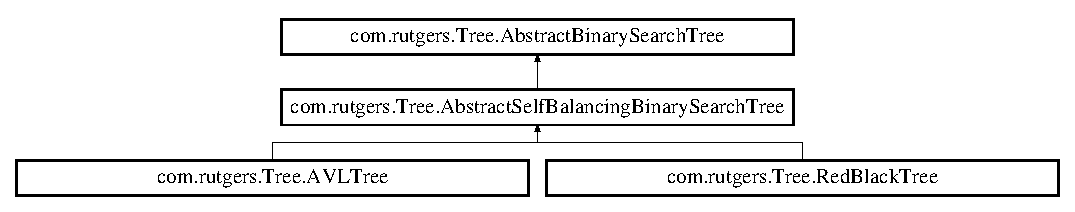
\includegraphics[height=2.400000cm]{classcom_1_1rutgers_1_1Tree_1_1AbstractBinarySearchTree}
\end{center}
\end{figure}
\subsection*{Public Member Functions}
\begin{DoxyCompactItemize}
\item 
Node \hyperlink{classcom_1_1rutgers_1_1Tree_1_1AbstractBinarySearchTree_a91602e347d8f02a67319b1bdc02ce60f}{search} (int element)
\item 
Node \hyperlink{classcom_1_1rutgers_1_1Tree_1_1AbstractBinarySearchTree_a0c7ca514dacdeb9085d258af23a7795e}{insert} (int element)
\item 
Node \hyperlink{classcom_1_1rutgers_1_1Tree_1_1AbstractBinarySearchTree_ae4be00a93f577025f71dd9560c11794b}{delete} (int element)
\item 
boolean \hyperlink{classcom_1_1rutgers_1_1Tree_1_1AbstractBinarySearchTree_a3fa83547331d30e71ef6906cfc67d686}{contains} (int element)
\item 
int \hyperlink{classcom_1_1rutgers_1_1Tree_1_1AbstractBinarySearchTree_a381c986a1e005fb07a5fb79d90218d79}{get\+Minimum} ()
\item 
int \hyperlink{classcom_1_1rutgers_1_1Tree_1_1AbstractBinarySearchTree_a19fac32887573d0c421ef6f191b694d1}{get\+Maximum} ()
\item 
int \hyperlink{classcom_1_1rutgers_1_1Tree_1_1AbstractBinarySearchTree_a91f7a4935262e9fd21035f3c795acbe1}{get\+Successor} (int element)
\item 
int \hyperlink{classcom_1_1rutgers_1_1Tree_1_1AbstractBinarySearchTree_a0d8f3f8b88ef6f741c0a0308f4ed0617}{get\+Size} ()
\item 
void \hyperlink{classcom_1_1rutgers_1_1Tree_1_1AbstractBinarySearchTree_a8757f96dff7c12848301f666fe2cc566}{print\+Tree\+In\+Order} ()
\item 
void \hyperlink{classcom_1_1rutgers_1_1Tree_1_1AbstractBinarySearchTree_a53e70e7883a86f60584f4585c07900ff}{print\+Tree\+Pre\+Order} ()
\item 
void \hyperlink{classcom_1_1rutgers_1_1Tree_1_1AbstractBinarySearchTree_a8efda65ce2fb4df01a22b7168882843a}{print\+Tree\+Post\+Order} ()
\end{DoxyCompactItemize}
\subsection*{Public Attributes}
\begin{DoxyCompactItemize}
\item 
Node \hyperlink{classcom_1_1rutgers_1_1Tree_1_1AbstractBinarySearchTree_aeeef22ff6ee25b6d8b9ceac2f17e8fe5}{root}
\end{DoxyCompactItemize}
\subsection*{Protected Member Functions}
\begin{DoxyCompactItemize}
\item 
abstract Node \hyperlink{classcom_1_1rutgers_1_1Tree_1_1AbstractBinarySearchTree_a4413dcd9175fd180bf7bd75aa0b94b73}{create\+Node} (int value, Node parent, Node left, Node right)
\item 
Node \hyperlink{classcom_1_1rutgers_1_1Tree_1_1AbstractBinarySearchTree_ab0b52e6fb9cdac67ef88ac7be48a3b60}{delete} (Node delete\+Node)
\end{DoxyCompactItemize}
\subsection*{Protected Attributes}
\begin{DoxyCompactItemize}
\item 
int \hyperlink{classcom_1_1rutgers_1_1Tree_1_1AbstractBinarySearchTree_aea91d533d1a9c4fa552c1625c50dd65d}{size}
\end{DoxyCompactItemize}


\subsection{Detailed Description}
\begin{DoxyAuthor}{Author}
eduard 
\end{DoxyAuthor}


\subsection{Member Function Documentation}
\mbox{\Hypertarget{classcom_1_1rutgers_1_1Tree_1_1AbstractBinarySearchTree_a3fa83547331d30e71ef6906cfc67d686}\label{classcom_1_1rutgers_1_1Tree_1_1AbstractBinarySearchTree_a3fa83547331d30e71ef6906cfc67d686}} 
\index{com\+::rutgers\+::\+Tree\+::\+Abstract\+Binary\+Search\+Tree@{com\+::rutgers\+::\+Tree\+::\+Abstract\+Binary\+Search\+Tree}!contains@{contains}}
\index{contains@{contains}!com\+::rutgers\+::\+Tree\+::\+Abstract\+Binary\+Search\+Tree@{com\+::rutgers\+::\+Tree\+::\+Abstract\+Binary\+Search\+Tree}}
\subsubsection{\texorpdfstring{contains()}{contains()}}
{\footnotesize\ttfamily boolean com.\+rutgers.\+Tree.\+Abstract\+Binary\+Search\+Tree.\+contains (\begin{DoxyParamCaption}\item[{int}]{element }\end{DoxyParamCaption})}


\begin{DoxyParams}{Parameters}
{\em element} & \\
\hline
\end{DoxyParams}
\begin{DoxyReturn}{Returns}
true if tree contains element. 
\end{DoxyReturn}
\mbox{\Hypertarget{classcom_1_1rutgers_1_1Tree_1_1AbstractBinarySearchTree_a4413dcd9175fd180bf7bd75aa0b94b73}\label{classcom_1_1rutgers_1_1Tree_1_1AbstractBinarySearchTree_a4413dcd9175fd180bf7bd75aa0b94b73}} 
\index{com\+::rutgers\+::\+Tree\+::\+Abstract\+Binary\+Search\+Tree@{com\+::rutgers\+::\+Tree\+::\+Abstract\+Binary\+Search\+Tree}!create\+Node@{create\+Node}}
\index{create\+Node@{create\+Node}!com\+::rutgers\+::\+Tree\+::\+Abstract\+Binary\+Search\+Tree@{com\+::rutgers\+::\+Tree\+::\+Abstract\+Binary\+Search\+Tree}}
\subsubsection{\texorpdfstring{create\+Node()}{createNode()}}
{\footnotesize\ttfamily abstract Node com.\+rutgers.\+Tree.\+Abstract\+Binary\+Search\+Tree.\+create\+Node (\begin{DoxyParamCaption}\item[{int}]{value,  }\item[{Node}]{parent,  }\item[{Node}]{left,  }\item[{Node}]{right }\end{DoxyParamCaption})\hspace{0.3cm}{\ttfamily [abstract]}, {\ttfamily [protected]}}

Because this is abstract class and various trees have different additional information on different nodes subclasses uses this abstract method to create nodes (maybe of class \hyperlink{}{Node} or maybe some different node sub class).


\begin{DoxyParams}{Parameters}
{\em value} & Value that node will have. \\
\hline
{\em parent} & Node\textquotesingle{}s parent. \\
\hline
{\em left} & Node\textquotesingle{}s left child. \\
\hline
{\em right} & Node\textquotesingle{}s right child. \\
\hline
\end{DoxyParams}
\begin{DoxyReturn}{Returns}
Created node instance. 
\end{DoxyReturn}
\mbox{\Hypertarget{classcom_1_1rutgers_1_1Tree_1_1AbstractBinarySearchTree_ae4be00a93f577025f71dd9560c11794b}\label{classcom_1_1rutgers_1_1Tree_1_1AbstractBinarySearchTree_ae4be00a93f577025f71dd9560c11794b}} 
\index{com\+::rutgers\+::\+Tree\+::\+Abstract\+Binary\+Search\+Tree@{com\+::rutgers\+::\+Tree\+::\+Abstract\+Binary\+Search\+Tree}!delete@{delete}}
\index{delete@{delete}!com\+::rutgers\+::\+Tree\+::\+Abstract\+Binary\+Search\+Tree@{com\+::rutgers\+::\+Tree\+::\+Abstract\+Binary\+Search\+Tree}}
\subsubsection{\texorpdfstring{delete()}{delete()}\hspace{0.1cm}{\footnotesize\ttfamily [1/2]}}
{\footnotesize\ttfamily Node com.\+rutgers.\+Tree.\+Abstract\+Binary\+Search\+Tree.\+delete (\begin{DoxyParamCaption}\item[{int}]{element }\end{DoxyParamCaption})}

Removes element if node with such value exists.


\begin{DoxyParams}{Parameters}
{\em element} & Element value to remove.\\
\hline
\end{DoxyParams}
\begin{DoxyReturn}{Returns}
New node that is in place of deleted node. Or null if element for delete was not found. 
\end{DoxyReturn}
\mbox{\Hypertarget{classcom_1_1rutgers_1_1Tree_1_1AbstractBinarySearchTree_ab0b52e6fb9cdac67ef88ac7be48a3b60}\label{classcom_1_1rutgers_1_1Tree_1_1AbstractBinarySearchTree_ab0b52e6fb9cdac67ef88ac7be48a3b60}} 
\index{com\+::rutgers\+::\+Tree\+::\+Abstract\+Binary\+Search\+Tree@{com\+::rutgers\+::\+Tree\+::\+Abstract\+Binary\+Search\+Tree}!delete@{delete}}
\index{delete@{delete}!com\+::rutgers\+::\+Tree\+::\+Abstract\+Binary\+Search\+Tree@{com\+::rutgers\+::\+Tree\+::\+Abstract\+Binary\+Search\+Tree}}
\subsubsection{\texorpdfstring{delete()}{delete()}\hspace{0.1cm}{\footnotesize\ttfamily [2/2]}}
{\footnotesize\ttfamily Node com.\+rutgers.\+Tree.\+Abstract\+Binary\+Search\+Tree.\+delete (\begin{DoxyParamCaption}\item[{Node}]{delete\+Node }\end{DoxyParamCaption})\hspace{0.3cm}{\ttfamily [protected]}}

Delete logic when node is already found.


\begin{DoxyParams}{Parameters}
{\em delete\+Node} & Node that needs to be deleted.\\
\hline
\end{DoxyParams}
\begin{DoxyReturn}{Returns}
New node that is in place of deleted node. Or null if element for delete was not found. 
\end{DoxyReturn}
\mbox{\Hypertarget{classcom_1_1rutgers_1_1Tree_1_1AbstractBinarySearchTree_a19fac32887573d0c421ef6f191b694d1}\label{classcom_1_1rutgers_1_1Tree_1_1AbstractBinarySearchTree_a19fac32887573d0c421ef6f191b694d1}} 
\index{com\+::rutgers\+::\+Tree\+::\+Abstract\+Binary\+Search\+Tree@{com\+::rutgers\+::\+Tree\+::\+Abstract\+Binary\+Search\+Tree}!get\+Maximum@{get\+Maximum}}
\index{get\+Maximum@{get\+Maximum}!com\+::rutgers\+::\+Tree\+::\+Abstract\+Binary\+Search\+Tree@{com\+::rutgers\+::\+Tree\+::\+Abstract\+Binary\+Search\+Tree}}
\subsubsection{\texorpdfstring{get\+Maximum()}{getMaximum()}}
{\footnotesize\ttfamily int com.\+rutgers.\+Tree.\+Abstract\+Binary\+Search\+Tree.\+get\+Maximum (\begin{DoxyParamCaption}{ }\end{DoxyParamCaption})}

\begin{DoxyReturn}{Returns}
Maximum element in tree. 
\end{DoxyReturn}
\mbox{\Hypertarget{classcom_1_1rutgers_1_1Tree_1_1AbstractBinarySearchTree_a381c986a1e005fb07a5fb79d90218d79}\label{classcom_1_1rutgers_1_1Tree_1_1AbstractBinarySearchTree_a381c986a1e005fb07a5fb79d90218d79}} 
\index{com\+::rutgers\+::\+Tree\+::\+Abstract\+Binary\+Search\+Tree@{com\+::rutgers\+::\+Tree\+::\+Abstract\+Binary\+Search\+Tree}!get\+Minimum@{get\+Minimum}}
\index{get\+Minimum@{get\+Minimum}!com\+::rutgers\+::\+Tree\+::\+Abstract\+Binary\+Search\+Tree@{com\+::rutgers\+::\+Tree\+::\+Abstract\+Binary\+Search\+Tree}}
\subsubsection{\texorpdfstring{get\+Minimum()}{getMinimum()}}
{\footnotesize\ttfamily int com.\+rutgers.\+Tree.\+Abstract\+Binary\+Search\+Tree.\+get\+Minimum (\begin{DoxyParamCaption}{ }\end{DoxyParamCaption})}

\begin{DoxyReturn}{Returns}
Minimum element in tree. 
\end{DoxyReturn}
\mbox{\Hypertarget{classcom_1_1rutgers_1_1Tree_1_1AbstractBinarySearchTree_a0d8f3f8b88ef6f741c0a0308f4ed0617}\label{classcom_1_1rutgers_1_1Tree_1_1AbstractBinarySearchTree_a0d8f3f8b88ef6f741c0a0308f4ed0617}} 
\index{com\+::rutgers\+::\+Tree\+::\+Abstract\+Binary\+Search\+Tree@{com\+::rutgers\+::\+Tree\+::\+Abstract\+Binary\+Search\+Tree}!get\+Size@{get\+Size}}
\index{get\+Size@{get\+Size}!com\+::rutgers\+::\+Tree\+::\+Abstract\+Binary\+Search\+Tree@{com\+::rutgers\+::\+Tree\+::\+Abstract\+Binary\+Search\+Tree}}
\subsubsection{\texorpdfstring{get\+Size()}{getSize()}}
{\footnotesize\ttfamily int com.\+rutgers.\+Tree.\+Abstract\+Binary\+Search\+Tree.\+get\+Size (\begin{DoxyParamCaption}{ }\end{DoxyParamCaption})}

\begin{DoxyReturn}{Returns}
Number of elements in the tree. 
\end{DoxyReturn}
\mbox{\Hypertarget{classcom_1_1rutgers_1_1Tree_1_1AbstractBinarySearchTree_a91f7a4935262e9fd21035f3c795acbe1}\label{classcom_1_1rutgers_1_1Tree_1_1AbstractBinarySearchTree_a91f7a4935262e9fd21035f3c795acbe1}} 
\index{com\+::rutgers\+::\+Tree\+::\+Abstract\+Binary\+Search\+Tree@{com\+::rutgers\+::\+Tree\+::\+Abstract\+Binary\+Search\+Tree}!get\+Successor@{get\+Successor}}
\index{get\+Successor@{get\+Successor}!com\+::rutgers\+::\+Tree\+::\+Abstract\+Binary\+Search\+Tree@{com\+::rutgers\+::\+Tree\+::\+Abstract\+Binary\+Search\+Tree}}
\subsubsection{\texorpdfstring{get\+Successor()}{getSuccessor()}}
{\footnotesize\ttfamily int com.\+rutgers.\+Tree.\+Abstract\+Binary\+Search\+Tree.\+get\+Successor (\begin{DoxyParamCaption}\item[{int}]{element }\end{DoxyParamCaption})}

Get next element element who is bigger than provided element.


\begin{DoxyParams}{Parameters}
{\em element} & Element for whom descendand element is searched \\
\hline
\end{DoxyParams}
\begin{DoxyReturn}{Returns}
Successor value. 
\end{DoxyReturn}
\mbox{\Hypertarget{classcom_1_1rutgers_1_1Tree_1_1AbstractBinarySearchTree_a0c7ca514dacdeb9085d258af23a7795e}\label{classcom_1_1rutgers_1_1Tree_1_1AbstractBinarySearchTree_a0c7ca514dacdeb9085d258af23a7795e}} 
\index{com\+::rutgers\+::\+Tree\+::\+Abstract\+Binary\+Search\+Tree@{com\+::rutgers\+::\+Tree\+::\+Abstract\+Binary\+Search\+Tree}!insert@{insert}}
\index{insert@{insert}!com\+::rutgers\+::\+Tree\+::\+Abstract\+Binary\+Search\+Tree@{com\+::rutgers\+::\+Tree\+::\+Abstract\+Binary\+Search\+Tree}}
\subsubsection{\texorpdfstring{insert()}{insert()}}
{\footnotesize\ttfamily Node com.\+rutgers.\+Tree.\+Abstract\+Binary\+Search\+Tree.\+insert (\begin{DoxyParamCaption}\item[{int}]{element }\end{DoxyParamCaption})}

Insert new element to tree.


\begin{DoxyParams}{Parameters}
{\em element} & Element to insert. \\
\hline
\end{DoxyParams}
\mbox{\Hypertarget{classcom_1_1rutgers_1_1Tree_1_1AbstractBinarySearchTree_a8757f96dff7c12848301f666fe2cc566}\label{classcom_1_1rutgers_1_1Tree_1_1AbstractBinarySearchTree_a8757f96dff7c12848301f666fe2cc566}} 
\index{com\+::rutgers\+::\+Tree\+::\+Abstract\+Binary\+Search\+Tree@{com\+::rutgers\+::\+Tree\+::\+Abstract\+Binary\+Search\+Tree}!print\+Tree\+In\+Order@{print\+Tree\+In\+Order}}
\index{print\+Tree\+In\+Order@{print\+Tree\+In\+Order}!com\+::rutgers\+::\+Tree\+::\+Abstract\+Binary\+Search\+Tree@{com\+::rutgers\+::\+Tree\+::\+Abstract\+Binary\+Search\+Tree}}
\subsubsection{\texorpdfstring{print\+Tree\+In\+Order()}{printTreeInOrder()}}
{\footnotesize\ttfamily void com.\+rutgers.\+Tree.\+Abstract\+Binary\+Search\+Tree.\+print\+Tree\+In\+Order (\begin{DoxyParamCaption}{ }\end{DoxyParamCaption})}

Tree traversal with printing element values. In order method. \mbox{\Hypertarget{classcom_1_1rutgers_1_1Tree_1_1AbstractBinarySearchTree_a8efda65ce2fb4df01a22b7168882843a}\label{classcom_1_1rutgers_1_1Tree_1_1AbstractBinarySearchTree_a8efda65ce2fb4df01a22b7168882843a}} 
\index{com\+::rutgers\+::\+Tree\+::\+Abstract\+Binary\+Search\+Tree@{com\+::rutgers\+::\+Tree\+::\+Abstract\+Binary\+Search\+Tree}!print\+Tree\+Post\+Order@{print\+Tree\+Post\+Order}}
\index{print\+Tree\+Post\+Order@{print\+Tree\+Post\+Order}!com\+::rutgers\+::\+Tree\+::\+Abstract\+Binary\+Search\+Tree@{com\+::rutgers\+::\+Tree\+::\+Abstract\+Binary\+Search\+Tree}}
\subsubsection{\texorpdfstring{print\+Tree\+Post\+Order()}{printTreePostOrder()}}
{\footnotesize\ttfamily void com.\+rutgers.\+Tree.\+Abstract\+Binary\+Search\+Tree.\+print\+Tree\+Post\+Order (\begin{DoxyParamCaption}{ }\end{DoxyParamCaption})}

Tree traversal with printing element values. Post order method. \mbox{\Hypertarget{classcom_1_1rutgers_1_1Tree_1_1AbstractBinarySearchTree_a53e70e7883a86f60584f4585c07900ff}\label{classcom_1_1rutgers_1_1Tree_1_1AbstractBinarySearchTree_a53e70e7883a86f60584f4585c07900ff}} 
\index{com\+::rutgers\+::\+Tree\+::\+Abstract\+Binary\+Search\+Tree@{com\+::rutgers\+::\+Tree\+::\+Abstract\+Binary\+Search\+Tree}!print\+Tree\+Pre\+Order@{print\+Tree\+Pre\+Order}}
\index{print\+Tree\+Pre\+Order@{print\+Tree\+Pre\+Order}!com\+::rutgers\+::\+Tree\+::\+Abstract\+Binary\+Search\+Tree@{com\+::rutgers\+::\+Tree\+::\+Abstract\+Binary\+Search\+Tree}}
\subsubsection{\texorpdfstring{print\+Tree\+Pre\+Order()}{printTreePreOrder()}}
{\footnotesize\ttfamily void com.\+rutgers.\+Tree.\+Abstract\+Binary\+Search\+Tree.\+print\+Tree\+Pre\+Order (\begin{DoxyParamCaption}{ }\end{DoxyParamCaption})}

Tree traversal with printing element values. Pre order method. \mbox{\Hypertarget{classcom_1_1rutgers_1_1Tree_1_1AbstractBinarySearchTree_a91602e347d8f02a67319b1bdc02ce60f}\label{classcom_1_1rutgers_1_1Tree_1_1AbstractBinarySearchTree_a91602e347d8f02a67319b1bdc02ce60f}} 
\index{com\+::rutgers\+::\+Tree\+::\+Abstract\+Binary\+Search\+Tree@{com\+::rutgers\+::\+Tree\+::\+Abstract\+Binary\+Search\+Tree}!search@{search}}
\index{search@{search}!com\+::rutgers\+::\+Tree\+::\+Abstract\+Binary\+Search\+Tree@{com\+::rutgers\+::\+Tree\+::\+Abstract\+Binary\+Search\+Tree}}
\subsubsection{\texorpdfstring{search()}{search()}}
{\footnotesize\ttfamily Node com.\+rutgers.\+Tree.\+Abstract\+Binary\+Search\+Tree.\+search (\begin{DoxyParamCaption}\item[{int}]{element }\end{DoxyParamCaption})}

Finds a node with concrete value. If it is not found then null is returned.


\begin{DoxyParams}{Parameters}
{\em element} & Element value. \\
\hline
\end{DoxyParams}
\begin{DoxyReturn}{Returns}
Node with value provided, or null if not found. 
\end{DoxyReturn}


\subsection{Member Data Documentation}
\mbox{\Hypertarget{classcom_1_1rutgers_1_1Tree_1_1AbstractBinarySearchTree_aeeef22ff6ee25b6d8b9ceac2f17e8fe5}\label{classcom_1_1rutgers_1_1Tree_1_1AbstractBinarySearchTree_aeeef22ff6ee25b6d8b9ceac2f17e8fe5}} 
\index{com\+::rutgers\+::\+Tree\+::\+Abstract\+Binary\+Search\+Tree@{com\+::rutgers\+::\+Tree\+::\+Abstract\+Binary\+Search\+Tree}!root@{root}}
\index{root@{root}!com\+::rutgers\+::\+Tree\+::\+Abstract\+Binary\+Search\+Tree@{com\+::rutgers\+::\+Tree\+::\+Abstract\+Binary\+Search\+Tree}}
\subsubsection{\texorpdfstring{root}{root}}
{\footnotesize\ttfamily Node com.\+rutgers.\+Tree.\+Abstract\+Binary\+Search\+Tree.\+root}

Root node where whole tree starts. \mbox{\Hypertarget{classcom_1_1rutgers_1_1Tree_1_1AbstractBinarySearchTree_aea91d533d1a9c4fa552c1625c50dd65d}\label{classcom_1_1rutgers_1_1Tree_1_1AbstractBinarySearchTree_aea91d533d1a9c4fa552c1625c50dd65d}} 
\index{com\+::rutgers\+::\+Tree\+::\+Abstract\+Binary\+Search\+Tree@{com\+::rutgers\+::\+Tree\+::\+Abstract\+Binary\+Search\+Tree}!size@{size}}
\index{size@{size}!com\+::rutgers\+::\+Tree\+::\+Abstract\+Binary\+Search\+Tree@{com\+::rutgers\+::\+Tree\+::\+Abstract\+Binary\+Search\+Tree}}
\subsubsection{\texorpdfstring{size}{size}}
{\footnotesize\ttfamily int com.\+rutgers.\+Tree.\+Abstract\+Binary\+Search\+Tree.\+size\hspace{0.3cm}{\ttfamily [protected]}}

Tree size. 

The documentation for this class was generated from the following file\+:\begin{DoxyCompactItemize}
\item 
src/main/java/com/rutgers/\+Tree/Abstract\+Binary\+Search\+Tree.\+java\end{DoxyCompactItemize}

\hypertarget{classcom_1_1rutgers_1_1QuadTree_1_1AbstractNode}{}\section{com.\+rutgers.\+Quad\+Tree.\+Abstract\+Node$<$ T $>$ Class Template Reference}
\label{classcom_1_1rutgers_1_1QuadTree_1_1AbstractNode}\index{com.\+rutgers.\+Quad\+Tree.\+Abstract\+Node$<$ T $>$@{com.\+rutgers.\+Quad\+Tree.\+Abstract\+Node$<$ T $>$}}
Inheritance diagram for com.\+rutgers.\+Quad\+Tree.\+Abstract\+Node$<$ T $>$\+:\begin{figure}[H]
\begin{center}
\leavevmode
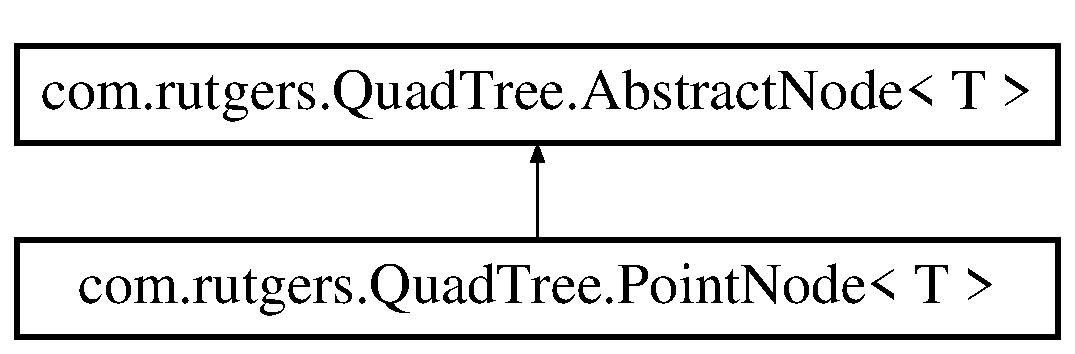
\includegraphics[height=2.000000cm]{classcom_1_1rutgers_1_1QuadTree_1_1AbstractNode}
\end{center}
\end{figure}
\subsection*{Public Member Functions}
\begin{DoxyCompactItemize}
\item 
double \hyperlink{classcom_1_1rutgers_1_1QuadTree_1_1AbstractNode_a0008c92d400cabb75304a86f79ef5ae4}{get\+North} ()
\item 
int \hyperlink{classcom_1_1rutgers_1_1QuadTree_1_1AbstractNode_af9a2b6025ac383b8ca8fd480519cde8a}{get\+Max\+Elements} ()
\item 
int \hyperlink{classcom_1_1rutgers_1_1QuadTree_1_1AbstractNode_ac3c4018f5d4369e09c58302bb9fa6012}{get\+Depth} ()
\item 
int \hyperlink{classcom_1_1rutgers_1_1QuadTree_1_1AbstractNode_a914674ce25b34e9818256028eabedf12}{get\+Max\+Depth} ()
\end{DoxyCompactItemize}
\subsection*{Static Protected Attributes}
\begin{DoxyCompactItemize}
\item 
static final int \hyperlink{classcom_1_1rutgers_1_1QuadTree_1_1AbstractNode_a3d1b2ce46d601ea32690b5d5e1706fd5}{M\+A\+X\+\_\+\+E\+L\+E\+M\+E\+N\+TS} = 4
\item 
static final int \hyperlink{classcom_1_1rutgers_1_1QuadTree_1_1AbstractNode_a72676d8499f815d16f4b8c72f3ac35c5}{M\+A\+X\+\_\+\+D\+E\+P\+TH} = 4
\end{DoxyCompactItemize}


\subsection{Detailed Description}
This class defined the Node that will be used in the Quad\+Tree.

\begin{DoxyAuthor}{Author}
Eduard Giber Renart 
\end{DoxyAuthor}
\begin{DoxyVersion}{Version}
1.\+0 
\end{DoxyVersion}


\subsection{Member Function Documentation}
\mbox{\Hypertarget{classcom_1_1rutgers_1_1QuadTree_1_1AbstractNode_ac3c4018f5d4369e09c58302bb9fa6012}\label{classcom_1_1rutgers_1_1QuadTree_1_1AbstractNode_ac3c4018f5d4369e09c58302bb9fa6012}} 
\index{com\+::rutgers\+::\+Quad\+Tree\+::\+Abstract\+Node@{com\+::rutgers\+::\+Quad\+Tree\+::\+Abstract\+Node}!get\+Depth@{get\+Depth}}
\index{get\+Depth@{get\+Depth}!com\+::rutgers\+::\+Quad\+Tree\+::\+Abstract\+Node@{com\+::rutgers\+::\+Quad\+Tree\+::\+Abstract\+Node}}
\subsubsection{\texorpdfstring{get\+Depth()}{getDepth()}}
{\footnotesize\ttfamily int \hyperlink{classcom_1_1rutgers_1_1QuadTree_1_1AbstractNode}{com.\+rutgers.\+Quad\+Tree.\+Abstract\+Node}$<$ T $>$.get\+Depth (\begin{DoxyParamCaption}{ }\end{DoxyParamCaption})}

Returns the depth of this node

\begin{DoxyReturn}{Returns}

\end{DoxyReturn}
\mbox{\Hypertarget{classcom_1_1rutgers_1_1QuadTree_1_1AbstractNode_a914674ce25b34e9818256028eabedf12}\label{classcom_1_1rutgers_1_1QuadTree_1_1AbstractNode_a914674ce25b34e9818256028eabedf12}} 
\index{com\+::rutgers\+::\+Quad\+Tree\+::\+Abstract\+Node@{com\+::rutgers\+::\+Quad\+Tree\+::\+Abstract\+Node}!get\+Max\+Depth@{get\+Max\+Depth}}
\index{get\+Max\+Depth@{get\+Max\+Depth}!com\+::rutgers\+::\+Quad\+Tree\+::\+Abstract\+Node@{com\+::rutgers\+::\+Quad\+Tree\+::\+Abstract\+Node}}
\subsubsection{\texorpdfstring{get\+Max\+Depth()}{getMaxDepth()}}
{\footnotesize\ttfamily int \hyperlink{classcom_1_1rutgers_1_1QuadTree_1_1AbstractNode}{com.\+rutgers.\+Quad\+Tree.\+Abstract\+Node}$<$ T $>$.get\+Max\+Depth (\begin{DoxyParamCaption}{ }\end{DoxyParamCaption})}

Returns the max depth

\begin{DoxyReturn}{Returns}

\end{DoxyReturn}
\mbox{\Hypertarget{classcom_1_1rutgers_1_1QuadTree_1_1AbstractNode_af9a2b6025ac383b8ca8fd480519cde8a}\label{classcom_1_1rutgers_1_1QuadTree_1_1AbstractNode_af9a2b6025ac383b8ca8fd480519cde8a}} 
\index{com\+::rutgers\+::\+Quad\+Tree\+::\+Abstract\+Node@{com\+::rutgers\+::\+Quad\+Tree\+::\+Abstract\+Node}!get\+Max\+Elements@{get\+Max\+Elements}}
\index{get\+Max\+Elements@{get\+Max\+Elements}!com\+::rutgers\+::\+Quad\+Tree\+::\+Abstract\+Node@{com\+::rutgers\+::\+Quad\+Tree\+::\+Abstract\+Node}}
\subsubsection{\texorpdfstring{get\+Max\+Elements()}{getMaxElements()}}
{\footnotesize\ttfamily int \hyperlink{classcom_1_1rutgers_1_1QuadTree_1_1AbstractNode}{com.\+rutgers.\+Quad\+Tree.\+Abstract\+Node}$<$ T $>$.get\+Max\+Elements (\begin{DoxyParamCaption}{ }\end{DoxyParamCaption})}

Returns the max elements

\begin{DoxyReturn}{Returns}

\end{DoxyReturn}
\mbox{\Hypertarget{classcom_1_1rutgers_1_1QuadTree_1_1AbstractNode_a0008c92d400cabb75304a86f79ef5ae4}\label{classcom_1_1rutgers_1_1QuadTree_1_1AbstractNode_a0008c92d400cabb75304a86f79ef5ae4}} 
\index{com\+::rutgers\+::\+Quad\+Tree\+::\+Abstract\+Node@{com\+::rutgers\+::\+Quad\+Tree\+::\+Abstract\+Node}!get\+North@{get\+North}}
\index{get\+North@{get\+North}!com\+::rutgers\+::\+Quad\+Tree\+::\+Abstract\+Node@{com\+::rutgers\+::\+Quad\+Tree\+::\+Abstract\+Node}}
\subsubsection{\texorpdfstring{get\+North()}{getNorth()}}
{\footnotesize\ttfamily double \hyperlink{classcom_1_1rutgers_1_1QuadTree_1_1AbstractNode}{com.\+rutgers.\+Quad\+Tree.\+Abstract\+Node}$<$ T $>$.get\+North (\begin{DoxyParamCaption}{ }\end{DoxyParamCaption})}

Returns the North

\begin{DoxyReturn}{Returns}

\end{DoxyReturn}


\subsection{Member Data Documentation}
\mbox{\Hypertarget{classcom_1_1rutgers_1_1QuadTree_1_1AbstractNode_a72676d8499f815d16f4b8c72f3ac35c5}\label{classcom_1_1rutgers_1_1QuadTree_1_1AbstractNode_a72676d8499f815d16f4b8c72f3ac35c5}} 
\index{com\+::rutgers\+::\+Quad\+Tree\+::\+Abstract\+Node@{com\+::rutgers\+::\+Quad\+Tree\+::\+Abstract\+Node}!M\+A\+X\+\_\+\+D\+E\+P\+TH@{M\+A\+X\+\_\+\+D\+E\+P\+TH}}
\index{M\+A\+X\+\_\+\+D\+E\+P\+TH@{M\+A\+X\+\_\+\+D\+E\+P\+TH}!com\+::rutgers\+::\+Quad\+Tree\+::\+Abstract\+Node@{com\+::rutgers\+::\+Quad\+Tree\+::\+Abstract\+Node}}
\subsubsection{\texorpdfstring{M\+A\+X\+\_\+\+D\+E\+P\+TH}{MAX\_DEPTH}}
{\footnotesize\ttfamily final int \hyperlink{classcom_1_1rutgers_1_1QuadTree_1_1AbstractNode}{com.\+rutgers.\+Quad\+Tree.\+Abstract\+Node}$<$ T $>$.M\+A\+X\+\_\+\+D\+E\+P\+TH = 4\hspace{0.3cm}{\ttfamily [static]}, {\ttfamily [protected]}}

Default value for max depth \mbox{\Hypertarget{classcom_1_1rutgers_1_1QuadTree_1_1AbstractNode_a3d1b2ce46d601ea32690b5d5e1706fd5}\label{classcom_1_1rutgers_1_1QuadTree_1_1AbstractNode_a3d1b2ce46d601ea32690b5d5e1706fd5}} 
\index{com\+::rutgers\+::\+Quad\+Tree\+::\+Abstract\+Node@{com\+::rutgers\+::\+Quad\+Tree\+::\+Abstract\+Node}!M\+A\+X\+\_\+\+E\+L\+E\+M\+E\+N\+TS@{M\+A\+X\+\_\+\+E\+L\+E\+M\+E\+N\+TS}}
\index{M\+A\+X\+\_\+\+E\+L\+E\+M\+E\+N\+TS@{M\+A\+X\+\_\+\+E\+L\+E\+M\+E\+N\+TS}!com\+::rutgers\+::\+Quad\+Tree\+::\+Abstract\+Node@{com\+::rutgers\+::\+Quad\+Tree\+::\+Abstract\+Node}}
\subsubsection{\texorpdfstring{M\+A\+X\+\_\+\+E\+L\+E\+M\+E\+N\+TS}{MAX\_ELEMENTS}}
{\footnotesize\ttfamily final int \hyperlink{classcom_1_1rutgers_1_1QuadTree_1_1AbstractNode}{com.\+rutgers.\+Quad\+Tree.\+Abstract\+Node}$<$ T $>$.M\+A\+X\+\_\+\+E\+L\+E\+M\+E\+N\+TS = 4\hspace{0.3cm}{\ttfamily [static]}, {\ttfamily [protected]}}

Default value for amount of elements 

The documentation for this class was generated from the following file\+:\begin{DoxyCompactItemize}
\item 
src/main/java/com/rutgers/\+Quad\+Tree/Abstract\+Node.\+java\end{DoxyCompactItemize}

\hypertarget{classcom_1_1rutgers_1_1QuadTree_1_1AbstractNodeElement}{}\section{com.\+rutgers.\+Quad\+Tree.\+Abstract\+Node\+Element$<$ T $>$ Class Template Reference}
\label{classcom_1_1rutgers_1_1QuadTree_1_1AbstractNodeElement}\index{com.\+rutgers.\+Quad\+Tree.\+Abstract\+Node\+Element$<$ T $>$@{com.\+rutgers.\+Quad\+Tree.\+Abstract\+Node\+Element$<$ T $>$}}
Inheritance diagram for com.\+rutgers.\+Quad\+Tree.\+Abstract\+Node\+Element$<$ T $>$\+:\begin{figure}[H]
\begin{center}
\leavevmode
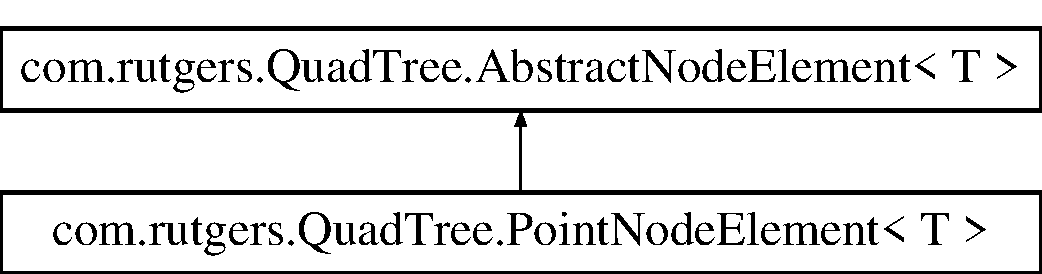
\includegraphics[height=2.000000cm]{classcom_1_1rutgers_1_1QuadTree_1_1AbstractNodeElement}
\end{center}
\end{figure}
\subsection*{Public Member Functions}
\begin{DoxyCompactItemize}
\item 
\hyperlink{classcom_1_1rutgers_1_1QuadTree_1_1AbstractNodeElement_ac5c8142d561f6f7f8c5c974164f4166a}{Abstract\+Node\+Element} (double latitude, double longitude, T element, String icon)
\item 
T \hyperlink{classcom_1_1rutgers_1_1QuadTree_1_1AbstractNodeElement_a8c24420f3c2acca151a1283773afd769}{get\+Element} ()
\end{DoxyCompactItemize}


\subsection{Detailed Description}
This class defines the Abstract Node Element

\begin{DoxyAuthor}{Author}
Eduard Giber Renart 
\end{DoxyAuthor}
\begin{DoxyVersion}{Version}
1.\+0 
\end{DoxyVersion}


\subsection{Constructor \& Destructor Documentation}
\mbox{\Hypertarget{classcom_1_1rutgers_1_1QuadTree_1_1AbstractNodeElement_ac5c8142d561f6f7f8c5c974164f4166a}\label{classcom_1_1rutgers_1_1QuadTree_1_1AbstractNodeElement_ac5c8142d561f6f7f8c5c974164f4166a}} 
\index{com\+::rutgers\+::\+Quad\+Tree\+::\+Abstract\+Node\+Element@{com\+::rutgers\+::\+Quad\+Tree\+::\+Abstract\+Node\+Element}!Abstract\+Node\+Element@{Abstract\+Node\+Element}}
\index{Abstract\+Node\+Element@{Abstract\+Node\+Element}!com\+::rutgers\+::\+Quad\+Tree\+::\+Abstract\+Node\+Element@{com\+::rutgers\+::\+Quad\+Tree\+::\+Abstract\+Node\+Element}}
\subsubsection{\texorpdfstring{Abstract\+Node\+Element()}{AbstractNodeElement()}}
{\footnotesize\ttfamily \hyperlink{classcom_1_1rutgers_1_1QuadTree_1_1AbstractNodeElement}{com.\+rutgers.\+Quad\+Tree.\+Abstract\+Node\+Element}$<$ T $>$.\hyperlink{classcom_1_1rutgers_1_1QuadTree_1_1AbstractNodeElement}{Abstract\+Node\+Element} (\begin{DoxyParamCaption}\item[{double}]{latitude,  }\item[{double}]{longitude,  }\item[{T}]{element,  }\item[{String}]{icon }\end{DoxyParamCaption})}

Create a new Node\+Element that holds the element at the given coordinates.


\begin{DoxyParams}{Parameters}
{\em x} & \\
\hline
{\em y} & \\
\hline
{\em element} & \\
\hline
\end{DoxyParams}


\subsection{Member Function Documentation}
\mbox{\Hypertarget{classcom_1_1rutgers_1_1QuadTree_1_1AbstractNodeElement_a8c24420f3c2acca151a1283773afd769}\label{classcom_1_1rutgers_1_1QuadTree_1_1AbstractNodeElement_a8c24420f3c2acca151a1283773afd769}} 
\index{com\+::rutgers\+::\+Quad\+Tree\+::\+Abstract\+Node\+Element@{com\+::rutgers\+::\+Quad\+Tree\+::\+Abstract\+Node\+Element}!get\+Element@{get\+Element}}
\index{get\+Element@{get\+Element}!com\+::rutgers\+::\+Quad\+Tree\+::\+Abstract\+Node\+Element@{com\+::rutgers\+::\+Quad\+Tree\+::\+Abstract\+Node\+Element}}
\subsubsection{\texorpdfstring{get\+Element()}{getElement()}}
{\footnotesize\ttfamily T \hyperlink{classcom_1_1rutgers_1_1QuadTree_1_1AbstractNodeElement}{com.\+rutgers.\+Quad\+Tree.\+Abstract\+Node\+Element}$<$ T $>$.get\+Element (\begin{DoxyParamCaption}{ }\end{DoxyParamCaption})}

Returns the element that is contained within this Node\+Element

\begin{DoxyReturn}{Returns}

\end{DoxyReturn}


The documentation for this class was generated from the following file\+:\begin{DoxyCompactItemize}
\item 
src/main/java/com/rutgers/\+Quad\+Tree/Abstract\+Node\+Element.\+java\end{DoxyCompactItemize}

\hypertarget{classcom_1_1rutgers_1_1QuadTree_1_1AbstractQuadTree}{}\section{com.\+rutgers.\+Quad\+Tree.\+Abstract\+Quad\+Tree$<$ T $>$ Class Template Reference}
\label{classcom_1_1rutgers_1_1QuadTree_1_1AbstractQuadTree}\index{com.\+rutgers.\+Quad\+Tree.\+Abstract\+Quad\+Tree$<$ T $>$@{com.\+rutgers.\+Quad\+Tree.\+Abstract\+Quad\+Tree$<$ T $>$}}
Inheritance diagram for com.\+rutgers.\+Quad\+Tree.\+Abstract\+Quad\+Tree$<$ T $>$\+:\begin{figure}[H]
\begin{center}
\leavevmode
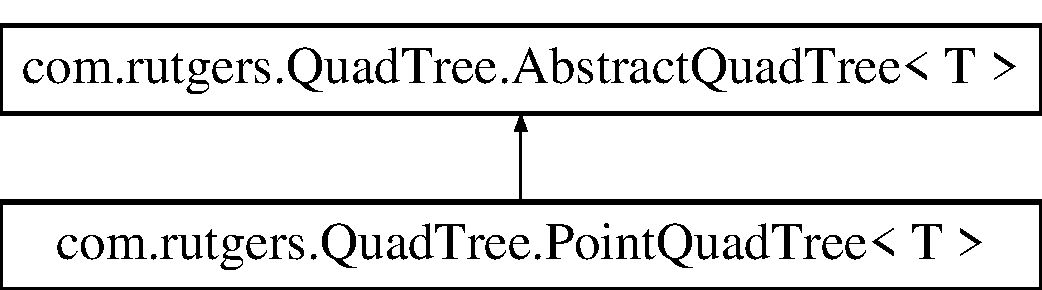
\includegraphics[height=2.000000cm]{classcom_1_1rutgers_1_1QuadTree_1_1AbstractQuadTree}
\end{center}
\end{figure}
\subsection*{Public Member Functions}
\begin{DoxyCompactItemize}
\item 
double \hyperlink{classcom_1_1rutgers_1_1QuadTree_1_1AbstractQuadTree_a83f2fde3929ecd03d905fd3e3fa72dc7}{get\+North} ()
\item 
abstract void \hyperlink{classcom_1_1rutgers_1_1QuadTree_1_1AbstractQuadTree_a0e4b7580a9924c3fad8409448730964a}{clear} ()
\item 
abstract \hyperlink{classcom_1_1rutgers_1_1QuadTree_1_1AbstractNode}{Abstract\+Node}$<$ T $>$ \hyperlink{classcom_1_1rutgers_1_1QuadTree_1_1AbstractQuadTree_a8cbaba782941b51f86c22b8109fa83e1}{get\+Root\+Node} ()
\end{DoxyCompactItemize}


\subsection{Detailed Description}
This class defines the \hyperlink{classcom_1_1rutgers_1_1QuadTree_1_1AbstractQuadTree}{Abstract\+Quad\+Tree}.

\begin{DoxyAuthor}{Author}
Eduard Giber Renart 
\end{DoxyAuthor}
\begin{DoxyVersion}{Version}
1.\+0 
\end{DoxyVersion}


\subsection{Member Function Documentation}
\mbox{\Hypertarget{classcom_1_1rutgers_1_1QuadTree_1_1AbstractQuadTree_a0e4b7580a9924c3fad8409448730964a}\label{classcom_1_1rutgers_1_1QuadTree_1_1AbstractQuadTree_a0e4b7580a9924c3fad8409448730964a}} 
\index{com\+::rutgers\+::\+Quad\+Tree\+::\+Abstract\+Quad\+Tree@{com\+::rutgers\+::\+Quad\+Tree\+::\+Abstract\+Quad\+Tree}!clear@{clear}}
\index{clear@{clear}!com\+::rutgers\+::\+Quad\+Tree\+::\+Abstract\+Quad\+Tree@{com\+::rutgers\+::\+Quad\+Tree\+::\+Abstract\+Quad\+Tree}}
\subsubsection{\texorpdfstring{clear()}{clear()}}
{\footnotesize\ttfamily abstract void \hyperlink{classcom_1_1rutgers_1_1QuadTree_1_1AbstractQuadTree}{com.\+rutgers.\+Quad\+Tree.\+Abstract\+Quad\+Tree}$<$ T $>$.clear (\begin{DoxyParamCaption}{ }\end{DoxyParamCaption})\hspace{0.3cm}{\ttfamily [abstract]}}

Clear the Quad\+Tree \mbox{\Hypertarget{classcom_1_1rutgers_1_1QuadTree_1_1AbstractQuadTree_a83f2fde3929ecd03d905fd3e3fa72dc7}\label{classcom_1_1rutgers_1_1QuadTree_1_1AbstractQuadTree_a83f2fde3929ecd03d905fd3e3fa72dc7}} 
\index{com\+::rutgers\+::\+Quad\+Tree\+::\+Abstract\+Quad\+Tree@{com\+::rutgers\+::\+Quad\+Tree\+::\+Abstract\+Quad\+Tree}!get\+North@{get\+North}}
\index{get\+North@{get\+North}!com\+::rutgers\+::\+Quad\+Tree\+::\+Abstract\+Quad\+Tree@{com\+::rutgers\+::\+Quad\+Tree\+::\+Abstract\+Quad\+Tree}}
\subsubsection{\texorpdfstring{get\+North()}{getNorth()}}
{\footnotesize\ttfamily double \hyperlink{classcom_1_1rutgers_1_1QuadTree_1_1AbstractQuadTree}{com.\+rutgers.\+Quad\+Tree.\+Abstract\+Quad\+Tree}$<$ T $>$.get\+North (\begin{DoxyParamCaption}{ }\end{DoxyParamCaption})}

Returns the north

\begin{DoxyReturn}{Returns}

\end{DoxyReturn}
\mbox{\Hypertarget{classcom_1_1rutgers_1_1QuadTree_1_1AbstractQuadTree_a8cbaba782941b51f86c22b8109fa83e1}\label{classcom_1_1rutgers_1_1QuadTree_1_1AbstractQuadTree_a8cbaba782941b51f86c22b8109fa83e1}} 
\index{com\+::rutgers\+::\+Quad\+Tree\+::\+Abstract\+Quad\+Tree@{com\+::rutgers\+::\+Quad\+Tree\+::\+Abstract\+Quad\+Tree}!get\+Root\+Node@{get\+Root\+Node}}
\index{get\+Root\+Node@{get\+Root\+Node}!com\+::rutgers\+::\+Quad\+Tree\+::\+Abstract\+Quad\+Tree@{com\+::rutgers\+::\+Quad\+Tree\+::\+Abstract\+Quad\+Tree}}
\subsubsection{\texorpdfstring{get\+Root\+Node()}{getRootNode()}}
{\footnotesize\ttfamily abstract \hyperlink{classcom_1_1rutgers_1_1QuadTree_1_1AbstractNode}{Abstract\+Node}$<$T$>$ \hyperlink{classcom_1_1rutgers_1_1QuadTree_1_1AbstractQuadTree}{com.\+rutgers.\+Quad\+Tree.\+Abstract\+Quad\+Tree}$<$ T $>$.get\+Root\+Node (\begin{DoxyParamCaption}{ }\end{DoxyParamCaption})\hspace{0.3cm}{\ttfamily [abstract]}}

Return the root node of this quad tree

\begin{DoxyReturn}{Returns}

\end{DoxyReturn}


The documentation for this class was generated from the following file\+:\begin{DoxyCompactItemize}
\item 
src/main/java/com/rutgers/\+Quad\+Tree/Abstract\+Quad\+Tree.\+java\end{DoxyCompactItemize}

\hypertarget{classcom_1_1rutgers_1_1Tree_1_1AbstractSelfBalancingBinarySearchTree}{}\section{com.\+rutgers.\+Tree.\+Abstract\+Self\+Balancing\+Binary\+Search\+Tree Class Reference}
\label{classcom_1_1rutgers_1_1Tree_1_1AbstractSelfBalancingBinarySearchTree}\index{com.\+rutgers.\+Tree.\+Abstract\+Self\+Balancing\+Binary\+Search\+Tree@{com.\+rutgers.\+Tree.\+Abstract\+Self\+Balancing\+Binary\+Search\+Tree}}
Inheritance diagram for com.\+rutgers.\+Tree.\+Abstract\+Self\+Balancing\+Binary\+Search\+Tree\+:\begin{figure}[H]
\begin{center}
\leavevmode
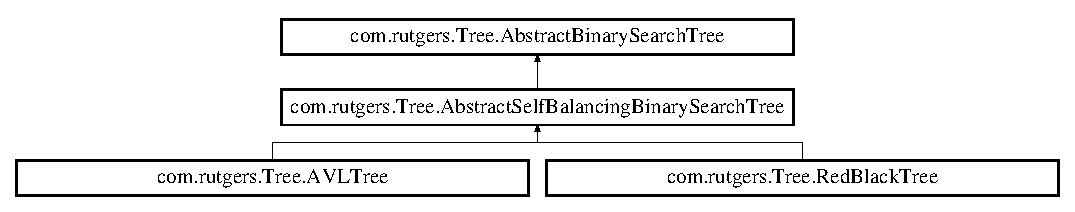
\includegraphics[height=2.400000cm]{classcom_1_1rutgers_1_1Tree_1_1AbstractSelfBalancingBinarySearchTree}
\end{center}
\end{figure}
\subsection*{Protected Member Functions}
\begin{DoxyCompactItemize}
\item 
Node \hyperlink{classcom_1_1rutgers_1_1Tree_1_1AbstractSelfBalancingBinarySearchTree_a143c3c90b0584ea35cd7b63f6172b4f4}{rotate\+Left} (Node node)
\item 
Node \hyperlink{classcom_1_1rutgers_1_1Tree_1_1AbstractSelfBalancingBinarySearchTree_a96bf5ab757164cf7fd2cf7cccff81276}{rotate\+Right} (Node node)
\end{DoxyCompactItemize}
\subsection*{Additional Inherited Members}


\subsection{Detailed Description}
\begin{DoxyAuthor}{Author}
eduard 
\end{DoxyAuthor}


\subsection{Member Function Documentation}
\mbox{\Hypertarget{classcom_1_1rutgers_1_1Tree_1_1AbstractSelfBalancingBinarySearchTree_a143c3c90b0584ea35cd7b63f6172b4f4}\label{classcom_1_1rutgers_1_1Tree_1_1AbstractSelfBalancingBinarySearchTree_a143c3c90b0584ea35cd7b63f6172b4f4}} 
\index{com\+::rutgers\+::\+Tree\+::\+Abstract\+Self\+Balancing\+Binary\+Search\+Tree@{com\+::rutgers\+::\+Tree\+::\+Abstract\+Self\+Balancing\+Binary\+Search\+Tree}!rotate\+Left@{rotate\+Left}}
\index{rotate\+Left@{rotate\+Left}!com\+::rutgers\+::\+Tree\+::\+Abstract\+Self\+Balancing\+Binary\+Search\+Tree@{com\+::rutgers\+::\+Tree\+::\+Abstract\+Self\+Balancing\+Binary\+Search\+Tree}}
\subsubsection{\texorpdfstring{rotate\+Left()}{rotateLeft()}}
{\footnotesize\ttfamily Node com.\+rutgers.\+Tree.\+Abstract\+Self\+Balancing\+Binary\+Search\+Tree.\+rotate\+Left (\begin{DoxyParamCaption}\item[{Node}]{node }\end{DoxyParamCaption})\hspace{0.3cm}{\ttfamily [protected]}}

Rotate to the left.


\begin{DoxyParams}{Parameters}
{\em node} & Node on which to rotate. \\
\hline
\end{DoxyParams}
\begin{DoxyReturn}{Returns}
Node that is in place of provided node after rotation. 
\end{DoxyReturn}
\mbox{\Hypertarget{classcom_1_1rutgers_1_1Tree_1_1AbstractSelfBalancingBinarySearchTree_a96bf5ab757164cf7fd2cf7cccff81276}\label{classcom_1_1rutgers_1_1Tree_1_1AbstractSelfBalancingBinarySearchTree_a96bf5ab757164cf7fd2cf7cccff81276}} 
\index{com\+::rutgers\+::\+Tree\+::\+Abstract\+Self\+Balancing\+Binary\+Search\+Tree@{com\+::rutgers\+::\+Tree\+::\+Abstract\+Self\+Balancing\+Binary\+Search\+Tree}!rotate\+Right@{rotate\+Right}}
\index{rotate\+Right@{rotate\+Right}!com\+::rutgers\+::\+Tree\+::\+Abstract\+Self\+Balancing\+Binary\+Search\+Tree@{com\+::rutgers\+::\+Tree\+::\+Abstract\+Self\+Balancing\+Binary\+Search\+Tree}}
\subsubsection{\texorpdfstring{rotate\+Right()}{rotateRight()}}
{\footnotesize\ttfamily Node com.\+rutgers.\+Tree.\+Abstract\+Self\+Balancing\+Binary\+Search\+Tree.\+rotate\+Right (\begin{DoxyParamCaption}\item[{Node}]{node }\end{DoxyParamCaption})\hspace{0.3cm}{\ttfamily [protected]}}

Rotate to the right.


\begin{DoxyParams}{Parameters}
{\em node} & Node on which to rotate. \\
\hline
\end{DoxyParams}
\begin{DoxyReturn}{Returns}
Node that is in place of provided node after rotation. 
\end{DoxyReturn}


The documentation for this class was generated from the following file\+:\begin{DoxyCompactItemize}
\item 
src/main/java/com/rutgers/\+Tree/Abstract\+Self\+Balancing\+Binary\+Search\+Tree.\+java\end{DoxyCompactItemize}

\hypertarget{enumcom_1_1rutgers_1_1Core_1_1Message_1_1ARMessage_1_1Action}{}\section{com.\+rutgers.\+Core.\+Message.\+A\+R\+Message.\+Action Enum Reference}
\label{enumcom_1_1rutgers_1_1Core_1_1Message_1_1ARMessage_1_1Action}\index{com.\+rutgers.\+Core.\+Message.\+A\+R\+Message.\+Action@{com.\+rutgers.\+Core.\+Message.\+A\+R\+Message.\+Action}}


Inherits Protocol\+Message\+Enum.

\subsection*{Static Public Member Functions}
\begin{DoxyCompactItemize}
\item 
.lang.\+Deprecated static \hyperlink{enumcom_1_1rutgers_1_1Core_1_1Message_1_1ARMessage_1_1Action}{Action} \hyperlink{enumcom_1_1rutgers_1_1Core_1_1Message_1_1ARMessage_1_1Action_a5c2fdd15663f6226c8df2565ea6cf998}{value\+Of} (int value)
\end{DoxyCompactItemize}
\subsection*{Public Attributes}
\begin{DoxyCompactItemize}
\item 
\hyperlink{enumcom_1_1rutgers_1_1Core_1_1Message_1_1ARMessage_1_1Action_a719992da108e69e6c1e8d6e4c60f64ce}{R\+E\+Q\+U\+E\+S\+T\+\_\+\+R\+E\+S\+P\+O\+N\+SE} =(0)
\item 
\hyperlink{enumcom_1_1rutgers_1_1Core_1_1Message_1_1ARMessage_1_1Action_ae567d96b2da0bf1c9a52680ad6b1b326}{S\+T\+O\+R\+E\+\_\+\+D\+A\+TA} =(1)
\item 
\hyperlink{enumcom_1_1rutgers_1_1Core_1_1Message_1_1ARMessage_1_1Action_a50a0de74e6895487cf6a7bdfe2b93edf}{S\+T\+O\+R\+E\+\_\+\+Q\+U\+E\+UE} =(2)
\item 
\hyperlink{enumcom_1_1rutgers_1_1Core_1_1Message_1_1ARMessage_1_1Action_a4a41d82033c2f13b62ed7156a60964da}{U\+P\+D\+A\+TE} =(3)
\item 
\hyperlink{enumcom_1_1rutgers_1_1Core_1_1Message_1_1ARMessage_1_1Action_a2d2d358b05ef21e959ce4d9761b11d9d}{R\+E\+Q\+U\+E\+ST} =(4)
\item 
\hyperlink{enumcom_1_1rutgers_1_1Core_1_1Message_1_1ARMessage_1_1Action_a52ac2f66a541aa4d91b8342abd757f9f}{H\+E\+L\+LO} =(5)
\item 
\hyperlink{enumcom_1_1rutgers_1_1Core_1_1Message_1_1ARMessage_1_1Action_a0ce49899d634232b0a754124a2f9b0e2}{N\+O\+T\+I\+F\+Y\+\_\+\+D\+A\+TA} =(6)
\item 
\hyperlink{enumcom_1_1rutgers_1_1Core_1_1Message_1_1ARMessage_1_1Action_a9c65fafb97fc3a5bc241aaadb1a07be3}{N\+O\+T\+I\+F\+Y\+\_\+\+I\+N\+T\+E\+R\+E\+ST} =(7)
\item 
\hyperlink{enumcom_1_1rutgers_1_1Core_1_1Message_1_1ARMessage_1_1Action_a6f3add60da0d6c7c7f13de17c672ac58}{N\+O\+T\+I\+F\+Y\+\_\+\+D\+A\+T\+A\+\_\+\+A\+N\+D\+R\+O\+ID} =(8)
\item 
\hyperlink{enumcom_1_1rutgers_1_1Core_1_1Message_1_1ARMessage_1_1Action_ab178e9fd8808bcfbad408871083cceae}{Q\+U\+E\+RY} =(9)
\item 
\hyperlink{enumcom_1_1rutgers_1_1Core_1_1Message_1_1ARMessage_1_1Action_a9377377b2dfe52bd9703e546a9d18026}{S\+T\+O\+R\+E\+\_\+\+S\+T\+O\+R\+M\+\_\+\+T\+O\+P\+O\+L\+O\+GY} =(10)
\item 
\hyperlink{enumcom_1_1rutgers_1_1Core_1_1Message_1_1ARMessage_1_1Action_a896c8085aa2da84ad92214e06dde8ab0}{S\+T\+A\+R\+T\+\_\+\+S\+T\+O\+R\+M\+\_\+\+T\+O\+P\+O\+L\+O\+GY} =(11)
\item 
\hyperlink{enumcom_1_1rutgers_1_1Core_1_1Message_1_1ARMessage_1_1Action_a0b3dd4140eb045a6f84fe487f2373e27}{S\+T\+O\+P\+\_\+\+S\+T\+O\+R\+M\+\_\+\+T\+O\+P\+O\+L\+O\+GY} =(12)
\item 
\hyperlink{enumcom_1_1rutgers_1_1Core_1_1Message_1_1ARMessage_1_1Action_a64d938ef2e15a0d2d3bf3a4b0f1ad421}{P\+R\+O\+F\+I\+L\+E\+\_\+\+R\+E\+Q\+U\+E\+ST} =(13)
\item 
\hyperlink{enumcom_1_1rutgers_1_1Core_1_1Message_1_1ARMessage_1_1Action_af08da2f44aad630ff583e7f5f51f4cfd}{P\+R\+O\+F\+I\+L\+E\+\_\+\+R\+E\+S\+P\+O\+N\+SE} =(14)
\item 
\hyperlink{enumcom_1_1rutgers_1_1Core_1_1Message_1_1ARMessage_1_1Action_a12bf1d5ab86f517d2df63bdc3a9b5506}{N\+O\+T\+I\+F\+Y\+\_\+\+S\+T\+A\+RT} =(15)
\item 
\hyperlink{enumcom_1_1rutgers_1_1Core_1_1Message_1_1ARMessage_1_1Action_acb3f41aefe125197dc119b316939759d}{N\+O\+T\+I\+F\+Y\+\_\+\+S\+T\+OP} =(16)
\item 
\hyperlink{enumcom_1_1rutgers_1_1Core_1_1Message_1_1ARMessage_1_1Action_a13340ac845ebf54c99021c2d6e258a77}{S\+T\+OP} =(17)
\item 
\hyperlink{enumcom_1_1rutgers_1_1Core_1_1Message_1_1ARMessage_1_1Action_a045685c23dcda10502b90997f9e4e2c8}{D\+E\+L\+E\+T\+E\+\_\+\+I\+N\+T\+E\+R\+E\+ST} =(18)
\item 
\hyperlink{enumcom_1_1rutgers_1_1Core_1_1Message_1_1ARMessage_1_1Action_a764c16f3474473262914da723c9d3562}{D\+E\+L\+E\+T\+E\+\_\+\+D\+A\+TA} =(19)
\item 
\hyperlink{enumcom_1_1rutgers_1_1Core_1_1Message_1_1ARMessage_1_1Action_a4fee38acd37c26881f193a3587645919}{S\+T\+O\+R\+E\+\_\+\+E\+D\+G\+E\+N\+T\+\_\+\+T\+O\+P\+O\+L\+O\+GY} =(20)
\item 
\hyperlink{enumcom_1_1rutgers_1_1Core_1_1Message_1_1ARMessage_1_1Action_a85e385507aa8578d36b6e3dc3399b269}{S\+T\+A\+R\+T\+\_\+\+E\+D\+G\+E\+N\+T\+\_\+\+T\+O\+P\+O\+L\+O\+GY} =(21)
\item 
\hyperlink{enumcom_1_1rutgers_1_1Core_1_1Message_1_1ARMessage_1_1Action_a8a75d2e395d6db96c236eb5e8a38a21e}{S\+T\+O\+P\+\_\+\+E\+D\+G\+E\+N\+T\+\_\+\+T\+O\+P\+O\+L\+O\+GY} =(22)
\end{DoxyCompactItemize}
\subsection*{Static Public Attributes}
\begin{DoxyCompactItemize}
\item 
static final int \hyperlink{enumcom_1_1rutgers_1_1Core_1_1Message_1_1ARMessage_1_1Action_a7535daaca4ea96d18c35c8b5a01b8378}{R\+E\+Q\+U\+E\+S\+T\+\_\+\+R\+E\+S\+P\+O\+N\+S\+E\+\_\+\+V\+A\+L\+UE} = 0
\item 
static final int \hyperlink{enumcom_1_1rutgers_1_1Core_1_1Message_1_1ARMessage_1_1Action_adbb69893c4ff87d2e8b9e92d90aec340}{S\+T\+O\+R\+E\+\_\+\+D\+A\+T\+A\+\_\+\+V\+A\+L\+UE} = 1
\item 
static final int \hyperlink{enumcom_1_1rutgers_1_1Core_1_1Message_1_1ARMessage_1_1Action_ab1008f6faf54881446e0a05c0ec8c35e}{S\+T\+O\+R\+E\+\_\+\+Q\+U\+E\+U\+E\+\_\+\+V\+A\+L\+UE} = 2
\item 
static final int \hyperlink{enumcom_1_1rutgers_1_1Core_1_1Message_1_1ARMessage_1_1Action_a23a05de08992c8780b16c71f602f062b}{U\+P\+D\+A\+T\+E\+\_\+\+V\+A\+L\+UE} = 3
\item 
static final int \hyperlink{enumcom_1_1rutgers_1_1Core_1_1Message_1_1ARMessage_1_1Action_aed1630c754d1d4ecb650dc8df0bf17e0}{R\+E\+Q\+U\+E\+S\+T\+\_\+\+V\+A\+L\+UE} = 4
\item 
static final int \hyperlink{enumcom_1_1rutgers_1_1Core_1_1Message_1_1ARMessage_1_1Action_abc5fdd737021d4a573f47b4c78163539}{H\+E\+L\+L\+O\+\_\+\+V\+A\+L\+UE} = 5
\item 
static final int \hyperlink{enumcom_1_1rutgers_1_1Core_1_1Message_1_1ARMessage_1_1Action_ad7f5b6bea782be4d992bb209bc674d17}{N\+O\+T\+I\+F\+Y\+\_\+\+D\+A\+T\+A\+\_\+\+V\+A\+L\+UE} = 6
\item 
static final int \hyperlink{enumcom_1_1rutgers_1_1Core_1_1Message_1_1ARMessage_1_1Action_a659c18e85873d2983c908b6bab4e40bf}{N\+O\+T\+I\+F\+Y\+\_\+\+I\+N\+T\+E\+R\+E\+S\+T\+\_\+\+V\+A\+L\+UE} = 7
\item 
static final int \hyperlink{enumcom_1_1rutgers_1_1Core_1_1Message_1_1ARMessage_1_1Action_af1a47bcb3a4907466f5fb518198319fd}{N\+O\+T\+I\+F\+Y\+\_\+\+D\+A\+T\+A\+\_\+\+A\+N\+D\+R\+O\+I\+D\+\_\+\+V\+A\+L\+UE} = 8
\item 
static final int \hyperlink{enumcom_1_1rutgers_1_1Core_1_1Message_1_1ARMessage_1_1Action_a63ee9318d02b99041a81b7ee2581abcf}{Q\+U\+E\+R\+Y\+\_\+\+V\+A\+L\+UE} = 9
\item 
static final int \hyperlink{enumcom_1_1rutgers_1_1Core_1_1Message_1_1ARMessage_1_1Action_a0b8ff174e309dc005416ac20bdc9e550}{S\+T\+O\+R\+E\+\_\+\+S\+T\+O\+R\+M\+\_\+\+T\+O\+P\+O\+L\+O\+G\+Y\+\_\+\+V\+A\+L\+UE} = 10
\item 
static final int \hyperlink{enumcom_1_1rutgers_1_1Core_1_1Message_1_1ARMessage_1_1Action_a586b51255fd4d3018fc72a7462ea7dc3}{S\+T\+A\+R\+T\+\_\+\+S\+T\+O\+R\+M\+\_\+\+T\+O\+P\+O\+L\+O\+G\+Y\+\_\+\+V\+A\+L\+UE} = 11
\item 
static final int \hyperlink{enumcom_1_1rutgers_1_1Core_1_1Message_1_1ARMessage_1_1Action_a5fefc8467945fc83716e26563ac2d48b}{S\+T\+O\+P\+\_\+\+S\+T\+O\+R\+M\+\_\+\+T\+O\+P\+O\+L\+O\+G\+Y\+\_\+\+V\+A\+L\+UE} = 12
\item 
static final int \hyperlink{enumcom_1_1rutgers_1_1Core_1_1Message_1_1ARMessage_1_1Action_a692f97c90a7315347e5e5744290fd1f8}{P\+R\+O\+F\+I\+L\+E\+\_\+\+R\+E\+Q\+U\+E\+S\+T\+\_\+\+V\+A\+L\+UE} = 13
\item 
static final int \hyperlink{enumcom_1_1rutgers_1_1Core_1_1Message_1_1ARMessage_1_1Action_a22bc9d9e2a9645fd8f49fc117783ea25}{P\+R\+O\+F\+I\+L\+E\+\_\+\+R\+E\+S\+P\+O\+N\+S\+E\+\_\+\+V\+A\+L\+UE} = 14
\item 
static final int \hyperlink{enumcom_1_1rutgers_1_1Core_1_1Message_1_1ARMessage_1_1Action_a85685fc746173f60de211c4262473427}{N\+O\+T\+I\+F\+Y\+\_\+\+S\+T\+A\+R\+T\+\_\+\+V\+A\+L\+UE} = 15
\item 
static final int \hyperlink{enumcom_1_1rutgers_1_1Core_1_1Message_1_1ARMessage_1_1Action_a355b310fc80fe14fea43b52d5271aab9}{N\+O\+T\+I\+F\+Y\+\_\+\+S\+T\+O\+P\+\_\+\+V\+A\+L\+UE} = 16
\item 
static final int \hyperlink{enumcom_1_1rutgers_1_1Core_1_1Message_1_1ARMessage_1_1Action_aa1fe7b3ad2ca3f7d72867e550feb6698}{S\+T\+O\+P\+\_\+\+V\+A\+L\+UE} = 17
\item 
static final int \hyperlink{enumcom_1_1rutgers_1_1Core_1_1Message_1_1ARMessage_1_1Action_adbcf2ca11eecbbf3932c004dc8d2f912}{D\+E\+L\+E\+T\+E\+\_\+\+I\+N\+T\+E\+R\+E\+S\+T\+\_\+\+V\+A\+L\+UE} = 18
\item 
static final int \hyperlink{enumcom_1_1rutgers_1_1Core_1_1Message_1_1ARMessage_1_1Action_a0a7492adcda5758f8db314dea768fae8}{D\+E\+L\+E\+T\+E\+\_\+\+D\+A\+T\+A\+\_\+\+V\+A\+L\+UE} = 19
\item 
static final int \hyperlink{enumcom_1_1rutgers_1_1Core_1_1Message_1_1ARMessage_1_1Action_ab4091e2dd07c1163797913c7f1c16f28}{S\+T\+O\+R\+E\+\_\+\+E\+D\+G\+E\+N\+T\+\_\+\+T\+O\+P\+O\+L\+O\+G\+Y\+\_\+\+V\+A\+L\+UE} = 20
\item 
static final int \hyperlink{enumcom_1_1rutgers_1_1Core_1_1Message_1_1ARMessage_1_1Action_a8d743cfa900cc77760ddb287fbcf00fd}{S\+T\+A\+R\+T\+\_\+\+E\+D\+G\+E\+N\+T\+\_\+\+T\+O\+P\+O\+L\+O\+G\+Y\+\_\+\+V\+A\+L\+UE} = 21
\item 
static final int \hyperlink{enumcom_1_1rutgers_1_1Core_1_1Message_1_1ARMessage_1_1Action_ac60c5616c039a74f3a98e348e0d2156b}{S\+T\+O\+P\+\_\+\+E\+D\+G\+E\+N\+T\+\_\+\+T\+O\+P\+O\+L\+O\+G\+Y\+\_\+\+V\+A\+L\+UE} = 22
\end{DoxyCompactItemize}


\subsection{Detailed Description}
Protobuf enum
\begin{DoxyCode}
tutorial.ARMessage.Action 
\end{DoxyCode}
 

\subsection{Member Function Documentation}
\mbox{\Hypertarget{enumcom_1_1rutgers_1_1Core_1_1Message_1_1ARMessage_1_1Action_a5c2fdd15663f6226c8df2565ea6cf998}\label{enumcom_1_1rutgers_1_1Core_1_1Message_1_1ARMessage_1_1Action_a5c2fdd15663f6226c8df2565ea6cf998}} 
\index{com\+::rutgers\+::\+Core\+::\+Message\+::\+A\+R\+Message\+::\+Action@{com\+::rutgers\+::\+Core\+::\+Message\+::\+A\+R\+Message\+::\+Action}!value\+Of@{value\+Of}}
\index{value\+Of@{value\+Of}!com\+::rutgers\+::\+Core\+::\+Message\+::\+A\+R\+Message\+::\+Action@{com\+::rutgers\+::\+Core\+::\+Message\+::\+A\+R\+Message\+::\+Action}}
\subsubsection{\texorpdfstring{value\+Of()}{valueOf()}}
{\footnotesize\ttfamily .lang.\+Deprecated static \hyperlink{enumcom_1_1rutgers_1_1Core_1_1Message_1_1ARMessage_1_1Action}{Action} com.\+rutgers.\+Core.\+Message.\+A\+R\+Message.\+Action.\+value\+Of (\begin{DoxyParamCaption}\item[{int}]{value }\end{DoxyParamCaption})\hspace{0.3cm}{\ttfamily [static]}}

\begin{DoxyRefDesc}{Deprecated}
\item[\hyperlink{deprecated__deprecated000002}{Deprecated}]Use \hyperlink{}{for\+Number(int)} instead. \end{DoxyRefDesc}


\subsection{Member Data Documentation}
\mbox{\Hypertarget{enumcom_1_1rutgers_1_1Core_1_1Message_1_1ARMessage_1_1Action_a764c16f3474473262914da723c9d3562}\label{enumcom_1_1rutgers_1_1Core_1_1Message_1_1ARMessage_1_1Action_a764c16f3474473262914da723c9d3562}} 
\index{com\+::rutgers\+::\+Core\+::\+Message\+::\+A\+R\+Message\+::\+Action@{com\+::rutgers\+::\+Core\+::\+Message\+::\+A\+R\+Message\+::\+Action}!D\+E\+L\+E\+T\+E\+\_\+\+D\+A\+TA@{D\+E\+L\+E\+T\+E\+\_\+\+D\+A\+TA}}
\index{D\+E\+L\+E\+T\+E\+\_\+\+D\+A\+TA@{D\+E\+L\+E\+T\+E\+\_\+\+D\+A\+TA}!com\+::rutgers\+::\+Core\+::\+Message\+::\+A\+R\+Message\+::\+Action@{com\+::rutgers\+::\+Core\+::\+Message\+::\+A\+R\+Message\+::\+Action}}
\subsubsection{\texorpdfstring{D\+E\+L\+E\+T\+E\+\_\+\+D\+A\+TA}{DELETE\_DATA}}
{\footnotesize\ttfamily com.\+rutgers.\+Core.\+Message.\+A\+R\+Message.\+Action.\+D\+E\+L\+E\+T\+E\+\_\+\+D\+A\+TA =(19)}

{\ttfamily D\+E\+L\+E\+T\+E\+\_\+\+D\+A\+TA = 19;} \mbox{\Hypertarget{enumcom_1_1rutgers_1_1Core_1_1Message_1_1ARMessage_1_1Action_a0a7492adcda5758f8db314dea768fae8}\label{enumcom_1_1rutgers_1_1Core_1_1Message_1_1ARMessage_1_1Action_a0a7492adcda5758f8db314dea768fae8}} 
\index{com\+::rutgers\+::\+Core\+::\+Message\+::\+A\+R\+Message\+::\+Action@{com\+::rutgers\+::\+Core\+::\+Message\+::\+A\+R\+Message\+::\+Action}!D\+E\+L\+E\+T\+E\+\_\+\+D\+A\+T\+A\+\_\+\+V\+A\+L\+UE@{D\+E\+L\+E\+T\+E\+\_\+\+D\+A\+T\+A\+\_\+\+V\+A\+L\+UE}}
\index{D\+E\+L\+E\+T\+E\+\_\+\+D\+A\+T\+A\+\_\+\+V\+A\+L\+UE@{D\+E\+L\+E\+T\+E\+\_\+\+D\+A\+T\+A\+\_\+\+V\+A\+L\+UE}!com\+::rutgers\+::\+Core\+::\+Message\+::\+A\+R\+Message\+::\+Action@{com\+::rutgers\+::\+Core\+::\+Message\+::\+A\+R\+Message\+::\+Action}}
\subsubsection{\texorpdfstring{D\+E\+L\+E\+T\+E\+\_\+\+D\+A\+T\+A\+\_\+\+V\+A\+L\+UE}{DELETE\_DATA\_VALUE}}
{\footnotesize\ttfamily  static  final int com.\+rutgers.\+Core.\+Message.\+A\+R\+Message.\+Action.\+D\+E\+L\+E\+T\+E\+\_\+\+D\+A\+T\+A\+\_\+\+V\+A\+L\+UE = 19\hspace{0.3cm}{\ttfamily [static]}}

{\ttfamily D\+E\+L\+E\+T\+E\+\_\+\+D\+A\+TA = 19;} \mbox{\Hypertarget{enumcom_1_1rutgers_1_1Core_1_1Message_1_1ARMessage_1_1Action_a045685c23dcda10502b90997f9e4e2c8}\label{enumcom_1_1rutgers_1_1Core_1_1Message_1_1ARMessage_1_1Action_a045685c23dcda10502b90997f9e4e2c8}} 
\index{com\+::rutgers\+::\+Core\+::\+Message\+::\+A\+R\+Message\+::\+Action@{com\+::rutgers\+::\+Core\+::\+Message\+::\+A\+R\+Message\+::\+Action}!D\+E\+L\+E\+T\+E\+\_\+\+I\+N\+T\+E\+R\+E\+ST@{D\+E\+L\+E\+T\+E\+\_\+\+I\+N\+T\+E\+R\+E\+ST}}
\index{D\+E\+L\+E\+T\+E\+\_\+\+I\+N\+T\+E\+R\+E\+ST@{D\+E\+L\+E\+T\+E\+\_\+\+I\+N\+T\+E\+R\+E\+ST}!com\+::rutgers\+::\+Core\+::\+Message\+::\+A\+R\+Message\+::\+Action@{com\+::rutgers\+::\+Core\+::\+Message\+::\+A\+R\+Message\+::\+Action}}
\subsubsection{\texorpdfstring{D\+E\+L\+E\+T\+E\+\_\+\+I\+N\+T\+E\+R\+E\+ST}{DELETE\_INTEREST}}
{\footnotesize\ttfamily com.\+rutgers.\+Core.\+Message.\+A\+R\+Message.\+Action.\+D\+E\+L\+E\+T\+E\+\_\+\+I\+N\+T\+E\+R\+E\+ST =(18)}

{\ttfamily D\+E\+L\+E\+T\+E\+\_\+\+I\+N\+T\+E\+R\+E\+ST = 18;} \mbox{\Hypertarget{enumcom_1_1rutgers_1_1Core_1_1Message_1_1ARMessage_1_1Action_adbcf2ca11eecbbf3932c004dc8d2f912}\label{enumcom_1_1rutgers_1_1Core_1_1Message_1_1ARMessage_1_1Action_adbcf2ca11eecbbf3932c004dc8d2f912}} 
\index{com\+::rutgers\+::\+Core\+::\+Message\+::\+A\+R\+Message\+::\+Action@{com\+::rutgers\+::\+Core\+::\+Message\+::\+A\+R\+Message\+::\+Action}!D\+E\+L\+E\+T\+E\+\_\+\+I\+N\+T\+E\+R\+E\+S\+T\+\_\+\+V\+A\+L\+UE@{D\+E\+L\+E\+T\+E\+\_\+\+I\+N\+T\+E\+R\+E\+S\+T\+\_\+\+V\+A\+L\+UE}}
\index{D\+E\+L\+E\+T\+E\+\_\+\+I\+N\+T\+E\+R\+E\+S\+T\+\_\+\+V\+A\+L\+UE@{D\+E\+L\+E\+T\+E\+\_\+\+I\+N\+T\+E\+R\+E\+S\+T\+\_\+\+V\+A\+L\+UE}!com\+::rutgers\+::\+Core\+::\+Message\+::\+A\+R\+Message\+::\+Action@{com\+::rutgers\+::\+Core\+::\+Message\+::\+A\+R\+Message\+::\+Action}}
\subsubsection{\texorpdfstring{D\+E\+L\+E\+T\+E\+\_\+\+I\+N\+T\+E\+R\+E\+S\+T\+\_\+\+V\+A\+L\+UE}{DELETE\_INTEREST\_VALUE}}
{\footnotesize\ttfamily  static  final int com.\+rutgers.\+Core.\+Message.\+A\+R\+Message.\+Action.\+D\+E\+L\+E\+T\+E\+\_\+\+I\+N\+T\+E\+R\+E\+S\+T\+\_\+\+V\+A\+L\+UE = 18\hspace{0.3cm}{\ttfamily [static]}}

{\ttfamily D\+E\+L\+E\+T\+E\+\_\+\+I\+N\+T\+E\+R\+E\+ST = 18;} \mbox{\Hypertarget{enumcom_1_1rutgers_1_1Core_1_1Message_1_1ARMessage_1_1Action_a52ac2f66a541aa4d91b8342abd757f9f}\label{enumcom_1_1rutgers_1_1Core_1_1Message_1_1ARMessage_1_1Action_a52ac2f66a541aa4d91b8342abd757f9f}} 
\index{com\+::rutgers\+::\+Core\+::\+Message\+::\+A\+R\+Message\+::\+Action@{com\+::rutgers\+::\+Core\+::\+Message\+::\+A\+R\+Message\+::\+Action}!H\+E\+L\+LO@{H\+E\+L\+LO}}
\index{H\+E\+L\+LO@{H\+E\+L\+LO}!com\+::rutgers\+::\+Core\+::\+Message\+::\+A\+R\+Message\+::\+Action@{com\+::rutgers\+::\+Core\+::\+Message\+::\+A\+R\+Message\+::\+Action}}
\subsubsection{\texorpdfstring{H\+E\+L\+LO}{HELLO}}
{\footnotesize\ttfamily com.\+rutgers.\+Core.\+Message.\+A\+R\+Message.\+Action.\+H\+E\+L\+LO =(5)}

{\ttfamily H\+E\+L\+LO = 5;} \mbox{\Hypertarget{enumcom_1_1rutgers_1_1Core_1_1Message_1_1ARMessage_1_1Action_abc5fdd737021d4a573f47b4c78163539}\label{enumcom_1_1rutgers_1_1Core_1_1Message_1_1ARMessage_1_1Action_abc5fdd737021d4a573f47b4c78163539}} 
\index{com\+::rutgers\+::\+Core\+::\+Message\+::\+A\+R\+Message\+::\+Action@{com\+::rutgers\+::\+Core\+::\+Message\+::\+A\+R\+Message\+::\+Action}!H\+E\+L\+L\+O\+\_\+\+V\+A\+L\+UE@{H\+E\+L\+L\+O\+\_\+\+V\+A\+L\+UE}}
\index{H\+E\+L\+L\+O\+\_\+\+V\+A\+L\+UE@{H\+E\+L\+L\+O\+\_\+\+V\+A\+L\+UE}!com\+::rutgers\+::\+Core\+::\+Message\+::\+A\+R\+Message\+::\+Action@{com\+::rutgers\+::\+Core\+::\+Message\+::\+A\+R\+Message\+::\+Action}}
\subsubsection{\texorpdfstring{H\+E\+L\+L\+O\+\_\+\+V\+A\+L\+UE}{HELLO\_VALUE}}
{\footnotesize\ttfamily  static  final int com.\+rutgers.\+Core.\+Message.\+A\+R\+Message.\+Action.\+H\+E\+L\+L\+O\+\_\+\+V\+A\+L\+UE = 5\hspace{0.3cm}{\ttfamily [static]}}

{\ttfamily H\+E\+L\+LO = 5;} \mbox{\Hypertarget{enumcom_1_1rutgers_1_1Core_1_1Message_1_1ARMessage_1_1Action_a0ce49899d634232b0a754124a2f9b0e2}\label{enumcom_1_1rutgers_1_1Core_1_1Message_1_1ARMessage_1_1Action_a0ce49899d634232b0a754124a2f9b0e2}} 
\index{com\+::rutgers\+::\+Core\+::\+Message\+::\+A\+R\+Message\+::\+Action@{com\+::rutgers\+::\+Core\+::\+Message\+::\+A\+R\+Message\+::\+Action}!N\+O\+T\+I\+F\+Y\+\_\+\+D\+A\+TA@{N\+O\+T\+I\+F\+Y\+\_\+\+D\+A\+TA}}
\index{N\+O\+T\+I\+F\+Y\+\_\+\+D\+A\+TA@{N\+O\+T\+I\+F\+Y\+\_\+\+D\+A\+TA}!com\+::rutgers\+::\+Core\+::\+Message\+::\+A\+R\+Message\+::\+Action@{com\+::rutgers\+::\+Core\+::\+Message\+::\+A\+R\+Message\+::\+Action}}
\subsubsection{\texorpdfstring{N\+O\+T\+I\+F\+Y\+\_\+\+D\+A\+TA}{NOTIFY\_DATA}}
{\footnotesize\ttfamily com.\+rutgers.\+Core.\+Message.\+A\+R\+Message.\+Action.\+N\+O\+T\+I\+F\+Y\+\_\+\+D\+A\+TA =(6)}

{\ttfamily N\+O\+T\+I\+F\+Y\+\_\+\+D\+A\+TA = 6;} \mbox{\Hypertarget{enumcom_1_1rutgers_1_1Core_1_1Message_1_1ARMessage_1_1Action_a6f3add60da0d6c7c7f13de17c672ac58}\label{enumcom_1_1rutgers_1_1Core_1_1Message_1_1ARMessage_1_1Action_a6f3add60da0d6c7c7f13de17c672ac58}} 
\index{com\+::rutgers\+::\+Core\+::\+Message\+::\+A\+R\+Message\+::\+Action@{com\+::rutgers\+::\+Core\+::\+Message\+::\+A\+R\+Message\+::\+Action}!N\+O\+T\+I\+F\+Y\+\_\+\+D\+A\+T\+A\+\_\+\+A\+N\+D\+R\+O\+ID@{N\+O\+T\+I\+F\+Y\+\_\+\+D\+A\+T\+A\+\_\+\+A\+N\+D\+R\+O\+ID}}
\index{N\+O\+T\+I\+F\+Y\+\_\+\+D\+A\+T\+A\+\_\+\+A\+N\+D\+R\+O\+ID@{N\+O\+T\+I\+F\+Y\+\_\+\+D\+A\+T\+A\+\_\+\+A\+N\+D\+R\+O\+ID}!com\+::rutgers\+::\+Core\+::\+Message\+::\+A\+R\+Message\+::\+Action@{com\+::rutgers\+::\+Core\+::\+Message\+::\+A\+R\+Message\+::\+Action}}
\subsubsection{\texorpdfstring{N\+O\+T\+I\+F\+Y\+\_\+\+D\+A\+T\+A\+\_\+\+A\+N\+D\+R\+O\+ID}{NOTIFY\_DATA\_ANDROID}}
{\footnotesize\ttfamily com.\+rutgers.\+Core.\+Message.\+A\+R\+Message.\+Action.\+N\+O\+T\+I\+F\+Y\+\_\+\+D\+A\+T\+A\+\_\+\+A\+N\+D\+R\+O\+ID =(8)}

{\ttfamily N\+O\+T\+I\+F\+Y\+\_\+\+D\+A\+T\+A\+\_\+\+A\+N\+D\+R\+O\+ID = 8;} \mbox{\Hypertarget{enumcom_1_1rutgers_1_1Core_1_1Message_1_1ARMessage_1_1Action_af1a47bcb3a4907466f5fb518198319fd}\label{enumcom_1_1rutgers_1_1Core_1_1Message_1_1ARMessage_1_1Action_af1a47bcb3a4907466f5fb518198319fd}} 
\index{com\+::rutgers\+::\+Core\+::\+Message\+::\+A\+R\+Message\+::\+Action@{com\+::rutgers\+::\+Core\+::\+Message\+::\+A\+R\+Message\+::\+Action}!N\+O\+T\+I\+F\+Y\+\_\+\+D\+A\+T\+A\+\_\+\+A\+N\+D\+R\+O\+I\+D\+\_\+\+V\+A\+L\+UE@{N\+O\+T\+I\+F\+Y\+\_\+\+D\+A\+T\+A\+\_\+\+A\+N\+D\+R\+O\+I\+D\+\_\+\+V\+A\+L\+UE}}
\index{N\+O\+T\+I\+F\+Y\+\_\+\+D\+A\+T\+A\+\_\+\+A\+N\+D\+R\+O\+I\+D\+\_\+\+V\+A\+L\+UE@{N\+O\+T\+I\+F\+Y\+\_\+\+D\+A\+T\+A\+\_\+\+A\+N\+D\+R\+O\+I\+D\+\_\+\+V\+A\+L\+UE}!com\+::rutgers\+::\+Core\+::\+Message\+::\+A\+R\+Message\+::\+Action@{com\+::rutgers\+::\+Core\+::\+Message\+::\+A\+R\+Message\+::\+Action}}
\subsubsection{\texorpdfstring{N\+O\+T\+I\+F\+Y\+\_\+\+D\+A\+T\+A\+\_\+\+A\+N\+D\+R\+O\+I\+D\+\_\+\+V\+A\+L\+UE}{NOTIFY\_DATA\_ANDROID\_VALUE}}
{\footnotesize\ttfamily  static  final int com.\+rutgers.\+Core.\+Message.\+A\+R\+Message.\+Action.\+N\+O\+T\+I\+F\+Y\+\_\+\+D\+A\+T\+A\+\_\+\+A\+N\+D\+R\+O\+I\+D\+\_\+\+V\+A\+L\+UE = 8\hspace{0.3cm}{\ttfamily [static]}}

{\ttfamily N\+O\+T\+I\+F\+Y\+\_\+\+D\+A\+T\+A\+\_\+\+A\+N\+D\+R\+O\+ID = 8;} \mbox{\Hypertarget{enumcom_1_1rutgers_1_1Core_1_1Message_1_1ARMessage_1_1Action_ad7f5b6bea782be4d992bb209bc674d17}\label{enumcom_1_1rutgers_1_1Core_1_1Message_1_1ARMessage_1_1Action_ad7f5b6bea782be4d992bb209bc674d17}} 
\index{com\+::rutgers\+::\+Core\+::\+Message\+::\+A\+R\+Message\+::\+Action@{com\+::rutgers\+::\+Core\+::\+Message\+::\+A\+R\+Message\+::\+Action}!N\+O\+T\+I\+F\+Y\+\_\+\+D\+A\+T\+A\+\_\+\+V\+A\+L\+UE@{N\+O\+T\+I\+F\+Y\+\_\+\+D\+A\+T\+A\+\_\+\+V\+A\+L\+UE}}
\index{N\+O\+T\+I\+F\+Y\+\_\+\+D\+A\+T\+A\+\_\+\+V\+A\+L\+UE@{N\+O\+T\+I\+F\+Y\+\_\+\+D\+A\+T\+A\+\_\+\+V\+A\+L\+UE}!com\+::rutgers\+::\+Core\+::\+Message\+::\+A\+R\+Message\+::\+Action@{com\+::rutgers\+::\+Core\+::\+Message\+::\+A\+R\+Message\+::\+Action}}
\subsubsection{\texorpdfstring{N\+O\+T\+I\+F\+Y\+\_\+\+D\+A\+T\+A\+\_\+\+V\+A\+L\+UE}{NOTIFY\_DATA\_VALUE}}
{\footnotesize\ttfamily  static  final int com.\+rutgers.\+Core.\+Message.\+A\+R\+Message.\+Action.\+N\+O\+T\+I\+F\+Y\+\_\+\+D\+A\+T\+A\+\_\+\+V\+A\+L\+UE = 6\hspace{0.3cm}{\ttfamily [static]}}

{\ttfamily N\+O\+T\+I\+F\+Y\+\_\+\+D\+A\+TA = 6;} \mbox{\Hypertarget{enumcom_1_1rutgers_1_1Core_1_1Message_1_1ARMessage_1_1Action_a9c65fafb97fc3a5bc241aaadb1a07be3}\label{enumcom_1_1rutgers_1_1Core_1_1Message_1_1ARMessage_1_1Action_a9c65fafb97fc3a5bc241aaadb1a07be3}} 
\index{com\+::rutgers\+::\+Core\+::\+Message\+::\+A\+R\+Message\+::\+Action@{com\+::rutgers\+::\+Core\+::\+Message\+::\+A\+R\+Message\+::\+Action}!N\+O\+T\+I\+F\+Y\+\_\+\+I\+N\+T\+E\+R\+E\+ST@{N\+O\+T\+I\+F\+Y\+\_\+\+I\+N\+T\+E\+R\+E\+ST}}
\index{N\+O\+T\+I\+F\+Y\+\_\+\+I\+N\+T\+E\+R\+E\+ST@{N\+O\+T\+I\+F\+Y\+\_\+\+I\+N\+T\+E\+R\+E\+ST}!com\+::rutgers\+::\+Core\+::\+Message\+::\+A\+R\+Message\+::\+Action@{com\+::rutgers\+::\+Core\+::\+Message\+::\+A\+R\+Message\+::\+Action}}
\subsubsection{\texorpdfstring{N\+O\+T\+I\+F\+Y\+\_\+\+I\+N\+T\+E\+R\+E\+ST}{NOTIFY\_INTEREST}}
{\footnotesize\ttfamily com.\+rutgers.\+Core.\+Message.\+A\+R\+Message.\+Action.\+N\+O\+T\+I\+F\+Y\+\_\+\+I\+N\+T\+E\+R\+E\+ST =(7)}

{\ttfamily N\+O\+T\+I\+F\+Y\+\_\+\+I\+N\+T\+E\+R\+E\+ST = 7;} \mbox{\Hypertarget{enumcom_1_1rutgers_1_1Core_1_1Message_1_1ARMessage_1_1Action_a659c18e85873d2983c908b6bab4e40bf}\label{enumcom_1_1rutgers_1_1Core_1_1Message_1_1ARMessage_1_1Action_a659c18e85873d2983c908b6bab4e40bf}} 
\index{com\+::rutgers\+::\+Core\+::\+Message\+::\+A\+R\+Message\+::\+Action@{com\+::rutgers\+::\+Core\+::\+Message\+::\+A\+R\+Message\+::\+Action}!N\+O\+T\+I\+F\+Y\+\_\+\+I\+N\+T\+E\+R\+E\+S\+T\+\_\+\+V\+A\+L\+UE@{N\+O\+T\+I\+F\+Y\+\_\+\+I\+N\+T\+E\+R\+E\+S\+T\+\_\+\+V\+A\+L\+UE}}
\index{N\+O\+T\+I\+F\+Y\+\_\+\+I\+N\+T\+E\+R\+E\+S\+T\+\_\+\+V\+A\+L\+UE@{N\+O\+T\+I\+F\+Y\+\_\+\+I\+N\+T\+E\+R\+E\+S\+T\+\_\+\+V\+A\+L\+UE}!com\+::rutgers\+::\+Core\+::\+Message\+::\+A\+R\+Message\+::\+Action@{com\+::rutgers\+::\+Core\+::\+Message\+::\+A\+R\+Message\+::\+Action}}
\subsubsection{\texorpdfstring{N\+O\+T\+I\+F\+Y\+\_\+\+I\+N\+T\+E\+R\+E\+S\+T\+\_\+\+V\+A\+L\+UE}{NOTIFY\_INTEREST\_VALUE}}
{\footnotesize\ttfamily  static  final int com.\+rutgers.\+Core.\+Message.\+A\+R\+Message.\+Action.\+N\+O\+T\+I\+F\+Y\+\_\+\+I\+N\+T\+E\+R\+E\+S\+T\+\_\+\+V\+A\+L\+UE = 7\hspace{0.3cm}{\ttfamily [static]}}

{\ttfamily N\+O\+T\+I\+F\+Y\+\_\+\+I\+N\+T\+E\+R\+E\+ST = 7;} \mbox{\Hypertarget{enumcom_1_1rutgers_1_1Core_1_1Message_1_1ARMessage_1_1Action_a12bf1d5ab86f517d2df63bdc3a9b5506}\label{enumcom_1_1rutgers_1_1Core_1_1Message_1_1ARMessage_1_1Action_a12bf1d5ab86f517d2df63bdc3a9b5506}} 
\index{com\+::rutgers\+::\+Core\+::\+Message\+::\+A\+R\+Message\+::\+Action@{com\+::rutgers\+::\+Core\+::\+Message\+::\+A\+R\+Message\+::\+Action}!N\+O\+T\+I\+F\+Y\+\_\+\+S\+T\+A\+RT@{N\+O\+T\+I\+F\+Y\+\_\+\+S\+T\+A\+RT}}
\index{N\+O\+T\+I\+F\+Y\+\_\+\+S\+T\+A\+RT@{N\+O\+T\+I\+F\+Y\+\_\+\+S\+T\+A\+RT}!com\+::rutgers\+::\+Core\+::\+Message\+::\+A\+R\+Message\+::\+Action@{com\+::rutgers\+::\+Core\+::\+Message\+::\+A\+R\+Message\+::\+Action}}
\subsubsection{\texorpdfstring{N\+O\+T\+I\+F\+Y\+\_\+\+S\+T\+A\+RT}{NOTIFY\_START}}
{\footnotesize\ttfamily com.\+rutgers.\+Core.\+Message.\+A\+R\+Message.\+Action.\+N\+O\+T\+I\+F\+Y\+\_\+\+S\+T\+A\+RT =(15)}

{\ttfamily N\+O\+T\+I\+F\+Y\+\_\+\+S\+T\+A\+RT = 15;} \mbox{\Hypertarget{enumcom_1_1rutgers_1_1Core_1_1Message_1_1ARMessage_1_1Action_a85685fc746173f60de211c4262473427}\label{enumcom_1_1rutgers_1_1Core_1_1Message_1_1ARMessage_1_1Action_a85685fc746173f60de211c4262473427}} 
\index{com\+::rutgers\+::\+Core\+::\+Message\+::\+A\+R\+Message\+::\+Action@{com\+::rutgers\+::\+Core\+::\+Message\+::\+A\+R\+Message\+::\+Action}!N\+O\+T\+I\+F\+Y\+\_\+\+S\+T\+A\+R\+T\+\_\+\+V\+A\+L\+UE@{N\+O\+T\+I\+F\+Y\+\_\+\+S\+T\+A\+R\+T\+\_\+\+V\+A\+L\+UE}}
\index{N\+O\+T\+I\+F\+Y\+\_\+\+S\+T\+A\+R\+T\+\_\+\+V\+A\+L\+UE@{N\+O\+T\+I\+F\+Y\+\_\+\+S\+T\+A\+R\+T\+\_\+\+V\+A\+L\+UE}!com\+::rutgers\+::\+Core\+::\+Message\+::\+A\+R\+Message\+::\+Action@{com\+::rutgers\+::\+Core\+::\+Message\+::\+A\+R\+Message\+::\+Action}}
\subsubsection{\texorpdfstring{N\+O\+T\+I\+F\+Y\+\_\+\+S\+T\+A\+R\+T\+\_\+\+V\+A\+L\+UE}{NOTIFY\_START\_VALUE}}
{\footnotesize\ttfamily  static  final int com.\+rutgers.\+Core.\+Message.\+A\+R\+Message.\+Action.\+N\+O\+T\+I\+F\+Y\+\_\+\+S\+T\+A\+R\+T\+\_\+\+V\+A\+L\+UE = 15\hspace{0.3cm}{\ttfamily [static]}}

{\ttfamily N\+O\+T\+I\+F\+Y\+\_\+\+S\+T\+A\+RT = 15;} \mbox{\Hypertarget{enumcom_1_1rutgers_1_1Core_1_1Message_1_1ARMessage_1_1Action_acb3f41aefe125197dc119b316939759d}\label{enumcom_1_1rutgers_1_1Core_1_1Message_1_1ARMessage_1_1Action_acb3f41aefe125197dc119b316939759d}} 
\index{com\+::rutgers\+::\+Core\+::\+Message\+::\+A\+R\+Message\+::\+Action@{com\+::rutgers\+::\+Core\+::\+Message\+::\+A\+R\+Message\+::\+Action}!N\+O\+T\+I\+F\+Y\+\_\+\+S\+T\+OP@{N\+O\+T\+I\+F\+Y\+\_\+\+S\+T\+OP}}
\index{N\+O\+T\+I\+F\+Y\+\_\+\+S\+T\+OP@{N\+O\+T\+I\+F\+Y\+\_\+\+S\+T\+OP}!com\+::rutgers\+::\+Core\+::\+Message\+::\+A\+R\+Message\+::\+Action@{com\+::rutgers\+::\+Core\+::\+Message\+::\+A\+R\+Message\+::\+Action}}
\subsubsection{\texorpdfstring{N\+O\+T\+I\+F\+Y\+\_\+\+S\+T\+OP}{NOTIFY\_STOP}}
{\footnotesize\ttfamily com.\+rutgers.\+Core.\+Message.\+A\+R\+Message.\+Action.\+N\+O\+T\+I\+F\+Y\+\_\+\+S\+T\+OP =(16)}

{\ttfamily N\+O\+T\+I\+F\+Y\+\_\+\+S\+T\+OP = 16;} \mbox{\Hypertarget{enumcom_1_1rutgers_1_1Core_1_1Message_1_1ARMessage_1_1Action_a355b310fc80fe14fea43b52d5271aab9}\label{enumcom_1_1rutgers_1_1Core_1_1Message_1_1ARMessage_1_1Action_a355b310fc80fe14fea43b52d5271aab9}} 
\index{com\+::rutgers\+::\+Core\+::\+Message\+::\+A\+R\+Message\+::\+Action@{com\+::rutgers\+::\+Core\+::\+Message\+::\+A\+R\+Message\+::\+Action}!N\+O\+T\+I\+F\+Y\+\_\+\+S\+T\+O\+P\+\_\+\+V\+A\+L\+UE@{N\+O\+T\+I\+F\+Y\+\_\+\+S\+T\+O\+P\+\_\+\+V\+A\+L\+UE}}
\index{N\+O\+T\+I\+F\+Y\+\_\+\+S\+T\+O\+P\+\_\+\+V\+A\+L\+UE@{N\+O\+T\+I\+F\+Y\+\_\+\+S\+T\+O\+P\+\_\+\+V\+A\+L\+UE}!com\+::rutgers\+::\+Core\+::\+Message\+::\+A\+R\+Message\+::\+Action@{com\+::rutgers\+::\+Core\+::\+Message\+::\+A\+R\+Message\+::\+Action}}
\subsubsection{\texorpdfstring{N\+O\+T\+I\+F\+Y\+\_\+\+S\+T\+O\+P\+\_\+\+V\+A\+L\+UE}{NOTIFY\_STOP\_VALUE}}
{\footnotesize\ttfamily  static  final int com.\+rutgers.\+Core.\+Message.\+A\+R\+Message.\+Action.\+N\+O\+T\+I\+F\+Y\+\_\+\+S\+T\+O\+P\+\_\+\+V\+A\+L\+UE = 16\hspace{0.3cm}{\ttfamily [static]}}

{\ttfamily N\+O\+T\+I\+F\+Y\+\_\+\+S\+T\+OP = 16;} \mbox{\Hypertarget{enumcom_1_1rutgers_1_1Core_1_1Message_1_1ARMessage_1_1Action_a64d938ef2e15a0d2d3bf3a4b0f1ad421}\label{enumcom_1_1rutgers_1_1Core_1_1Message_1_1ARMessage_1_1Action_a64d938ef2e15a0d2d3bf3a4b0f1ad421}} 
\index{com\+::rutgers\+::\+Core\+::\+Message\+::\+A\+R\+Message\+::\+Action@{com\+::rutgers\+::\+Core\+::\+Message\+::\+A\+R\+Message\+::\+Action}!P\+R\+O\+F\+I\+L\+E\+\_\+\+R\+E\+Q\+U\+E\+ST@{P\+R\+O\+F\+I\+L\+E\+\_\+\+R\+E\+Q\+U\+E\+ST}}
\index{P\+R\+O\+F\+I\+L\+E\+\_\+\+R\+E\+Q\+U\+E\+ST@{P\+R\+O\+F\+I\+L\+E\+\_\+\+R\+E\+Q\+U\+E\+ST}!com\+::rutgers\+::\+Core\+::\+Message\+::\+A\+R\+Message\+::\+Action@{com\+::rutgers\+::\+Core\+::\+Message\+::\+A\+R\+Message\+::\+Action}}
\subsubsection{\texorpdfstring{P\+R\+O\+F\+I\+L\+E\+\_\+\+R\+E\+Q\+U\+E\+ST}{PROFILE\_REQUEST}}
{\footnotesize\ttfamily com.\+rutgers.\+Core.\+Message.\+A\+R\+Message.\+Action.\+P\+R\+O\+F\+I\+L\+E\+\_\+\+R\+E\+Q\+U\+E\+ST =(13)}

{\ttfamily P\+R\+O\+F\+I\+L\+E\+\_\+\+R\+E\+Q\+U\+E\+ST = 13;} \mbox{\Hypertarget{enumcom_1_1rutgers_1_1Core_1_1Message_1_1ARMessage_1_1Action_a692f97c90a7315347e5e5744290fd1f8}\label{enumcom_1_1rutgers_1_1Core_1_1Message_1_1ARMessage_1_1Action_a692f97c90a7315347e5e5744290fd1f8}} 
\index{com\+::rutgers\+::\+Core\+::\+Message\+::\+A\+R\+Message\+::\+Action@{com\+::rutgers\+::\+Core\+::\+Message\+::\+A\+R\+Message\+::\+Action}!P\+R\+O\+F\+I\+L\+E\+\_\+\+R\+E\+Q\+U\+E\+S\+T\+\_\+\+V\+A\+L\+UE@{P\+R\+O\+F\+I\+L\+E\+\_\+\+R\+E\+Q\+U\+E\+S\+T\+\_\+\+V\+A\+L\+UE}}
\index{P\+R\+O\+F\+I\+L\+E\+\_\+\+R\+E\+Q\+U\+E\+S\+T\+\_\+\+V\+A\+L\+UE@{P\+R\+O\+F\+I\+L\+E\+\_\+\+R\+E\+Q\+U\+E\+S\+T\+\_\+\+V\+A\+L\+UE}!com\+::rutgers\+::\+Core\+::\+Message\+::\+A\+R\+Message\+::\+Action@{com\+::rutgers\+::\+Core\+::\+Message\+::\+A\+R\+Message\+::\+Action}}
\subsubsection{\texorpdfstring{P\+R\+O\+F\+I\+L\+E\+\_\+\+R\+E\+Q\+U\+E\+S\+T\+\_\+\+V\+A\+L\+UE}{PROFILE\_REQUEST\_VALUE}}
{\footnotesize\ttfamily  static  final int com.\+rutgers.\+Core.\+Message.\+A\+R\+Message.\+Action.\+P\+R\+O\+F\+I\+L\+E\+\_\+\+R\+E\+Q\+U\+E\+S\+T\+\_\+\+V\+A\+L\+UE = 13\hspace{0.3cm}{\ttfamily [static]}}

{\ttfamily P\+R\+O\+F\+I\+L\+E\+\_\+\+R\+E\+Q\+U\+E\+ST = 13;} \mbox{\Hypertarget{enumcom_1_1rutgers_1_1Core_1_1Message_1_1ARMessage_1_1Action_af08da2f44aad630ff583e7f5f51f4cfd}\label{enumcom_1_1rutgers_1_1Core_1_1Message_1_1ARMessage_1_1Action_af08da2f44aad630ff583e7f5f51f4cfd}} 
\index{com\+::rutgers\+::\+Core\+::\+Message\+::\+A\+R\+Message\+::\+Action@{com\+::rutgers\+::\+Core\+::\+Message\+::\+A\+R\+Message\+::\+Action}!P\+R\+O\+F\+I\+L\+E\+\_\+\+R\+E\+S\+P\+O\+N\+SE@{P\+R\+O\+F\+I\+L\+E\+\_\+\+R\+E\+S\+P\+O\+N\+SE}}
\index{P\+R\+O\+F\+I\+L\+E\+\_\+\+R\+E\+S\+P\+O\+N\+SE@{P\+R\+O\+F\+I\+L\+E\+\_\+\+R\+E\+S\+P\+O\+N\+SE}!com\+::rutgers\+::\+Core\+::\+Message\+::\+A\+R\+Message\+::\+Action@{com\+::rutgers\+::\+Core\+::\+Message\+::\+A\+R\+Message\+::\+Action}}
\subsubsection{\texorpdfstring{P\+R\+O\+F\+I\+L\+E\+\_\+\+R\+E\+S\+P\+O\+N\+SE}{PROFILE\_RESPONSE}}
{\footnotesize\ttfamily com.\+rutgers.\+Core.\+Message.\+A\+R\+Message.\+Action.\+P\+R\+O\+F\+I\+L\+E\+\_\+\+R\+E\+S\+P\+O\+N\+SE =(14)}

{\ttfamily P\+R\+O\+F\+I\+L\+E\+\_\+\+R\+E\+S\+P\+O\+N\+SE = 14;} \mbox{\Hypertarget{enumcom_1_1rutgers_1_1Core_1_1Message_1_1ARMessage_1_1Action_a22bc9d9e2a9645fd8f49fc117783ea25}\label{enumcom_1_1rutgers_1_1Core_1_1Message_1_1ARMessage_1_1Action_a22bc9d9e2a9645fd8f49fc117783ea25}} 
\index{com\+::rutgers\+::\+Core\+::\+Message\+::\+A\+R\+Message\+::\+Action@{com\+::rutgers\+::\+Core\+::\+Message\+::\+A\+R\+Message\+::\+Action}!P\+R\+O\+F\+I\+L\+E\+\_\+\+R\+E\+S\+P\+O\+N\+S\+E\+\_\+\+V\+A\+L\+UE@{P\+R\+O\+F\+I\+L\+E\+\_\+\+R\+E\+S\+P\+O\+N\+S\+E\+\_\+\+V\+A\+L\+UE}}
\index{P\+R\+O\+F\+I\+L\+E\+\_\+\+R\+E\+S\+P\+O\+N\+S\+E\+\_\+\+V\+A\+L\+UE@{P\+R\+O\+F\+I\+L\+E\+\_\+\+R\+E\+S\+P\+O\+N\+S\+E\+\_\+\+V\+A\+L\+UE}!com\+::rutgers\+::\+Core\+::\+Message\+::\+A\+R\+Message\+::\+Action@{com\+::rutgers\+::\+Core\+::\+Message\+::\+A\+R\+Message\+::\+Action}}
\subsubsection{\texorpdfstring{P\+R\+O\+F\+I\+L\+E\+\_\+\+R\+E\+S\+P\+O\+N\+S\+E\+\_\+\+V\+A\+L\+UE}{PROFILE\_RESPONSE\_VALUE}}
{\footnotesize\ttfamily  static  final int com.\+rutgers.\+Core.\+Message.\+A\+R\+Message.\+Action.\+P\+R\+O\+F\+I\+L\+E\+\_\+\+R\+E\+S\+P\+O\+N\+S\+E\+\_\+\+V\+A\+L\+UE = 14\hspace{0.3cm}{\ttfamily [static]}}

{\ttfamily P\+R\+O\+F\+I\+L\+E\+\_\+\+R\+E\+S\+P\+O\+N\+SE = 14;} \mbox{\Hypertarget{enumcom_1_1rutgers_1_1Core_1_1Message_1_1ARMessage_1_1Action_ab178e9fd8808bcfbad408871083cceae}\label{enumcom_1_1rutgers_1_1Core_1_1Message_1_1ARMessage_1_1Action_ab178e9fd8808bcfbad408871083cceae}} 
\index{com\+::rutgers\+::\+Core\+::\+Message\+::\+A\+R\+Message\+::\+Action@{com\+::rutgers\+::\+Core\+::\+Message\+::\+A\+R\+Message\+::\+Action}!Q\+U\+E\+RY@{Q\+U\+E\+RY}}
\index{Q\+U\+E\+RY@{Q\+U\+E\+RY}!com\+::rutgers\+::\+Core\+::\+Message\+::\+A\+R\+Message\+::\+Action@{com\+::rutgers\+::\+Core\+::\+Message\+::\+A\+R\+Message\+::\+Action}}
\subsubsection{\texorpdfstring{Q\+U\+E\+RY}{QUERY}}
{\footnotesize\ttfamily com.\+rutgers.\+Core.\+Message.\+A\+R\+Message.\+Action.\+Q\+U\+E\+RY =(9)}

{\ttfamily Q\+U\+E\+RY = 9;} \mbox{\Hypertarget{enumcom_1_1rutgers_1_1Core_1_1Message_1_1ARMessage_1_1Action_a63ee9318d02b99041a81b7ee2581abcf}\label{enumcom_1_1rutgers_1_1Core_1_1Message_1_1ARMessage_1_1Action_a63ee9318d02b99041a81b7ee2581abcf}} 
\index{com\+::rutgers\+::\+Core\+::\+Message\+::\+A\+R\+Message\+::\+Action@{com\+::rutgers\+::\+Core\+::\+Message\+::\+A\+R\+Message\+::\+Action}!Q\+U\+E\+R\+Y\+\_\+\+V\+A\+L\+UE@{Q\+U\+E\+R\+Y\+\_\+\+V\+A\+L\+UE}}
\index{Q\+U\+E\+R\+Y\+\_\+\+V\+A\+L\+UE@{Q\+U\+E\+R\+Y\+\_\+\+V\+A\+L\+UE}!com\+::rutgers\+::\+Core\+::\+Message\+::\+A\+R\+Message\+::\+Action@{com\+::rutgers\+::\+Core\+::\+Message\+::\+A\+R\+Message\+::\+Action}}
\subsubsection{\texorpdfstring{Q\+U\+E\+R\+Y\+\_\+\+V\+A\+L\+UE}{QUERY\_VALUE}}
{\footnotesize\ttfamily  static  final int com.\+rutgers.\+Core.\+Message.\+A\+R\+Message.\+Action.\+Q\+U\+E\+R\+Y\+\_\+\+V\+A\+L\+UE = 9\hspace{0.3cm}{\ttfamily [static]}}

{\ttfamily Q\+U\+E\+RY = 9;} \mbox{\Hypertarget{enumcom_1_1rutgers_1_1Core_1_1Message_1_1ARMessage_1_1Action_a2d2d358b05ef21e959ce4d9761b11d9d}\label{enumcom_1_1rutgers_1_1Core_1_1Message_1_1ARMessage_1_1Action_a2d2d358b05ef21e959ce4d9761b11d9d}} 
\index{com\+::rutgers\+::\+Core\+::\+Message\+::\+A\+R\+Message\+::\+Action@{com\+::rutgers\+::\+Core\+::\+Message\+::\+A\+R\+Message\+::\+Action}!R\+E\+Q\+U\+E\+ST@{R\+E\+Q\+U\+E\+ST}}
\index{R\+E\+Q\+U\+E\+ST@{R\+E\+Q\+U\+E\+ST}!com\+::rutgers\+::\+Core\+::\+Message\+::\+A\+R\+Message\+::\+Action@{com\+::rutgers\+::\+Core\+::\+Message\+::\+A\+R\+Message\+::\+Action}}
\subsubsection{\texorpdfstring{R\+E\+Q\+U\+E\+ST}{REQUEST}}
{\footnotesize\ttfamily com.\+rutgers.\+Core.\+Message.\+A\+R\+Message.\+Action.\+R\+E\+Q\+U\+E\+ST =(4)}

{\ttfamily R\+E\+Q\+U\+E\+ST = 4;} \mbox{\Hypertarget{enumcom_1_1rutgers_1_1Core_1_1Message_1_1ARMessage_1_1Action_a719992da108e69e6c1e8d6e4c60f64ce}\label{enumcom_1_1rutgers_1_1Core_1_1Message_1_1ARMessage_1_1Action_a719992da108e69e6c1e8d6e4c60f64ce}} 
\index{com\+::rutgers\+::\+Core\+::\+Message\+::\+A\+R\+Message\+::\+Action@{com\+::rutgers\+::\+Core\+::\+Message\+::\+A\+R\+Message\+::\+Action}!R\+E\+Q\+U\+E\+S\+T\+\_\+\+R\+E\+S\+P\+O\+N\+SE@{R\+E\+Q\+U\+E\+S\+T\+\_\+\+R\+E\+S\+P\+O\+N\+SE}}
\index{R\+E\+Q\+U\+E\+S\+T\+\_\+\+R\+E\+S\+P\+O\+N\+SE@{R\+E\+Q\+U\+E\+S\+T\+\_\+\+R\+E\+S\+P\+O\+N\+SE}!com\+::rutgers\+::\+Core\+::\+Message\+::\+A\+R\+Message\+::\+Action@{com\+::rutgers\+::\+Core\+::\+Message\+::\+A\+R\+Message\+::\+Action}}
\subsubsection{\texorpdfstring{R\+E\+Q\+U\+E\+S\+T\+\_\+\+R\+E\+S\+P\+O\+N\+SE}{REQUEST\_RESPONSE}}
{\footnotesize\ttfamily com.\+rutgers.\+Core.\+Message.\+A\+R\+Message.\+Action.\+R\+E\+Q\+U\+E\+S\+T\+\_\+\+R\+E\+S\+P\+O\+N\+SE =(0)}

{\ttfamily R\+E\+Q\+U\+E\+S\+T\+\_\+\+R\+E\+S\+P\+O\+N\+SE = 0;} \mbox{\Hypertarget{enumcom_1_1rutgers_1_1Core_1_1Message_1_1ARMessage_1_1Action_a7535daaca4ea96d18c35c8b5a01b8378}\label{enumcom_1_1rutgers_1_1Core_1_1Message_1_1ARMessage_1_1Action_a7535daaca4ea96d18c35c8b5a01b8378}} 
\index{com\+::rutgers\+::\+Core\+::\+Message\+::\+A\+R\+Message\+::\+Action@{com\+::rutgers\+::\+Core\+::\+Message\+::\+A\+R\+Message\+::\+Action}!R\+E\+Q\+U\+E\+S\+T\+\_\+\+R\+E\+S\+P\+O\+N\+S\+E\+\_\+\+V\+A\+L\+UE@{R\+E\+Q\+U\+E\+S\+T\+\_\+\+R\+E\+S\+P\+O\+N\+S\+E\+\_\+\+V\+A\+L\+UE}}
\index{R\+E\+Q\+U\+E\+S\+T\+\_\+\+R\+E\+S\+P\+O\+N\+S\+E\+\_\+\+V\+A\+L\+UE@{R\+E\+Q\+U\+E\+S\+T\+\_\+\+R\+E\+S\+P\+O\+N\+S\+E\+\_\+\+V\+A\+L\+UE}!com\+::rutgers\+::\+Core\+::\+Message\+::\+A\+R\+Message\+::\+Action@{com\+::rutgers\+::\+Core\+::\+Message\+::\+A\+R\+Message\+::\+Action}}
\subsubsection{\texorpdfstring{R\+E\+Q\+U\+E\+S\+T\+\_\+\+R\+E\+S\+P\+O\+N\+S\+E\+\_\+\+V\+A\+L\+UE}{REQUEST\_RESPONSE\_VALUE}}
{\footnotesize\ttfamily  static  final int com.\+rutgers.\+Core.\+Message.\+A\+R\+Message.\+Action.\+R\+E\+Q\+U\+E\+S\+T\+\_\+\+R\+E\+S\+P\+O\+N\+S\+E\+\_\+\+V\+A\+L\+UE = 0\hspace{0.3cm}{\ttfamily [static]}}

{\ttfamily R\+E\+Q\+U\+E\+S\+T\+\_\+\+R\+E\+S\+P\+O\+N\+SE = 0;} \mbox{\Hypertarget{enumcom_1_1rutgers_1_1Core_1_1Message_1_1ARMessage_1_1Action_aed1630c754d1d4ecb650dc8df0bf17e0}\label{enumcom_1_1rutgers_1_1Core_1_1Message_1_1ARMessage_1_1Action_aed1630c754d1d4ecb650dc8df0bf17e0}} 
\index{com\+::rutgers\+::\+Core\+::\+Message\+::\+A\+R\+Message\+::\+Action@{com\+::rutgers\+::\+Core\+::\+Message\+::\+A\+R\+Message\+::\+Action}!R\+E\+Q\+U\+E\+S\+T\+\_\+\+V\+A\+L\+UE@{R\+E\+Q\+U\+E\+S\+T\+\_\+\+V\+A\+L\+UE}}
\index{R\+E\+Q\+U\+E\+S\+T\+\_\+\+V\+A\+L\+UE@{R\+E\+Q\+U\+E\+S\+T\+\_\+\+V\+A\+L\+UE}!com\+::rutgers\+::\+Core\+::\+Message\+::\+A\+R\+Message\+::\+Action@{com\+::rutgers\+::\+Core\+::\+Message\+::\+A\+R\+Message\+::\+Action}}
\subsubsection{\texorpdfstring{R\+E\+Q\+U\+E\+S\+T\+\_\+\+V\+A\+L\+UE}{REQUEST\_VALUE}}
{\footnotesize\ttfamily  static  final int com.\+rutgers.\+Core.\+Message.\+A\+R\+Message.\+Action.\+R\+E\+Q\+U\+E\+S\+T\+\_\+\+V\+A\+L\+UE = 4\hspace{0.3cm}{\ttfamily [static]}}

{\ttfamily R\+E\+Q\+U\+E\+ST = 4;} \mbox{\Hypertarget{enumcom_1_1rutgers_1_1Core_1_1Message_1_1ARMessage_1_1Action_a85e385507aa8578d36b6e3dc3399b269}\label{enumcom_1_1rutgers_1_1Core_1_1Message_1_1ARMessage_1_1Action_a85e385507aa8578d36b6e3dc3399b269}} 
\index{com\+::rutgers\+::\+Core\+::\+Message\+::\+A\+R\+Message\+::\+Action@{com\+::rutgers\+::\+Core\+::\+Message\+::\+A\+R\+Message\+::\+Action}!S\+T\+A\+R\+T\+\_\+\+E\+D\+G\+E\+N\+T\+\_\+\+T\+O\+P\+O\+L\+O\+GY@{S\+T\+A\+R\+T\+\_\+\+E\+D\+G\+E\+N\+T\+\_\+\+T\+O\+P\+O\+L\+O\+GY}}
\index{S\+T\+A\+R\+T\+\_\+\+E\+D\+G\+E\+N\+T\+\_\+\+T\+O\+P\+O\+L\+O\+GY@{S\+T\+A\+R\+T\+\_\+\+E\+D\+G\+E\+N\+T\+\_\+\+T\+O\+P\+O\+L\+O\+GY}!com\+::rutgers\+::\+Core\+::\+Message\+::\+A\+R\+Message\+::\+Action@{com\+::rutgers\+::\+Core\+::\+Message\+::\+A\+R\+Message\+::\+Action}}
\subsubsection{\texorpdfstring{S\+T\+A\+R\+T\+\_\+\+E\+D\+G\+E\+N\+T\+\_\+\+T\+O\+P\+O\+L\+O\+GY}{START\_EDGENT\_TOPOLOGY}}
{\footnotesize\ttfamily com.\+rutgers.\+Core.\+Message.\+A\+R\+Message.\+Action.\+S\+T\+A\+R\+T\+\_\+\+E\+D\+G\+E\+N\+T\+\_\+\+T\+O\+P\+O\+L\+O\+GY =(21)}

{\ttfamily S\+T\+A\+R\+T\+\_\+\+E\+D\+G\+E\+N\+T\+\_\+\+T\+O\+P\+O\+L\+O\+GY = 21;} \mbox{\Hypertarget{enumcom_1_1rutgers_1_1Core_1_1Message_1_1ARMessage_1_1Action_a8d743cfa900cc77760ddb287fbcf00fd}\label{enumcom_1_1rutgers_1_1Core_1_1Message_1_1ARMessage_1_1Action_a8d743cfa900cc77760ddb287fbcf00fd}} 
\index{com\+::rutgers\+::\+Core\+::\+Message\+::\+A\+R\+Message\+::\+Action@{com\+::rutgers\+::\+Core\+::\+Message\+::\+A\+R\+Message\+::\+Action}!S\+T\+A\+R\+T\+\_\+\+E\+D\+G\+E\+N\+T\+\_\+\+T\+O\+P\+O\+L\+O\+G\+Y\+\_\+\+V\+A\+L\+UE@{S\+T\+A\+R\+T\+\_\+\+E\+D\+G\+E\+N\+T\+\_\+\+T\+O\+P\+O\+L\+O\+G\+Y\+\_\+\+V\+A\+L\+UE}}
\index{S\+T\+A\+R\+T\+\_\+\+E\+D\+G\+E\+N\+T\+\_\+\+T\+O\+P\+O\+L\+O\+G\+Y\+\_\+\+V\+A\+L\+UE@{S\+T\+A\+R\+T\+\_\+\+E\+D\+G\+E\+N\+T\+\_\+\+T\+O\+P\+O\+L\+O\+G\+Y\+\_\+\+V\+A\+L\+UE}!com\+::rutgers\+::\+Core\+::\+Message\+::\+A\+R\+Message\+::\+Action@{com\+::rutgers\+::\+Core\+::\+Message\+::\+A\+R\+Message\+::\+Action}}
\subsubsection{\texorpdfstring{S\+T\+A\+R\+T\+\_\+\+E\+D\+G\+E\+N\+T\+\_\+\+T\+O\+P\+O\+L\+O\+G\+Y\+\_\+\+V\+A\+L\+UE}{START\_EDGENT\_TOPOLOGY\_VALUE}}
{\footnotesize\ttfamily  static  final int com.\+rutgers.\+Core.\+Message.\+A\+R\+Message.\+Action.\+S\+T\+A\+R\+T\+\_\+\+E\+D\+G\+E\+N\+T\+\_\+\+T\+O\+P\+O\+L\+O\+G\+Y\+\_\+\+V\+A\+L\+UE = 21\hspace{0.3cm}{\ttfamily [static]}}

{\ttfamily S\+T\+A\+R\+T\+\_\+\+E\+D\+G\+E\+N\+T\+\_\+\+T\+O\+P\+O\+L\+O\+GY = 21;} \mbox{\Hypertarget{enumcom_1_1rutgers_1_1Core_1_1Message_1_1ARMessage_1_1Action_a896c8085aa2da84ad92214e06dde8ab0}\label{enumcom_1_1rutgers_1_1Core_1_1Message_1_1ARMessage_1_1Action_a896c8085aa2da84ad92214e06dde8ab0}} 
\index{com\+::rutgers\+::\+Core\+::\+Message\+::\+A\+R\+Message\+::\+Action@{com\+::rutgers\+::\+Core\+::\+Message\+::\+A\+R\+Message\+::\+Action}!S\+T\+A\+R\+T\+\_\+\+S\+T\+O\+R\+M\+\_\+\+T\+O\+P\+O\+L\+O\+GY@{S\+T\+A\+R\+T\+\_\+\+S\+T\+O\+R\+M\+\_\+\+T\+O\+P\+O\+L\+O\+GY}}
\index{S\+T\+A\+R\+T\+\_\+\+S\+T\+O\+R\+M\+\_\+\+T\+O\+P\+O\+L\+O\+GY@{S\+T\+A\+R\+T\+\_\+\+S\+T\+O\+R\+M\+\_\+\+T\+O\+P\+O\+L\+O\+GY}!com\+::rutgers\+::\+Core\+::\+Message\+::\+A\+R\+Message\+::\+Action@{com\+::rutgers\+::\+Core\+::\+Message\+::\+A\+R\+Message\+::\+Action}}
\subsubsection{\texorpdfstring{S\+T\+A\+R\+T\+\_\+\+S\+T\+O\+R\+M\+\_\+\+T\+O\+P\+O\+L\+O\+GY}{START\_STORM\_TOPOLOGY}}
{\footnotesize\ttfamily com.\+rutgers.\+Core.\+Message.\+A\+R\+Message.\+Action.\+S\+T\+A\+R\+T\+\_\+\+S\+T\+O\+R\+M\+\_\+\+T\+O\+P\+O\+L\+O\+GY =(11)}

{\ttfamily S\+T\+A\+R\+T\+\_\+\+S\+T\+O\+R\+M\+\_\+\+T\+O\+P\+O\+L\+O\+GY = 11;} \mbox{\Hypertarget{enumcom_1_1rutgers_1_1Core_1_1Message_1_1ARMessage_1_1Action_a586b51255fd4d3018fc72a7462ea7dc3}\label{enumcom_1_1rutgers_1_1Core_1_1Message_1_1ARMessage_1_1Action_a586b51255fd4d3018fc72a7462ea7dc3}} 
\index{com\+::rutgers\+::\+Core\+::\+Message\+::\+A\+R\+Message\+::\+Action@{com\+::rutgers\+::\+Core\+::\+Message\+::\+A\+R\+Message\+::\+Action}!S\+T\+A\+R\+T\+\_\+\+S\+T\+O\+R\+M\+\_\+\+T\+O\+P\+O\+L\+O\+G\+Y\+\_\+\+V\+A\+L\+UE@{S\+T\+A\+R\+T\+\_\+\+S\+T\+O\+R\+M\+\_\+\+T\+O\+P\+O\+L\+O\+G\+Y\+\_\+\+V\+A\+L\+UE}}
\index{S\+T\+A\+R\+T\+\_\+\+S\+T\+O\+R\+M\+\_\+\+T\+O\+P\+O\+L\+O\+G\+Y\+\_\+\+V\+A\+L\+UE@{S\+T\+A\+R\+T\+\_\+\+S\+T\+O\+R\+M\+\_\+\+T\+O\+P\+O\+L\+O\+G\+Y\+\_\+\+V\+A\+L\+UE}!com\+::rutgers\+::\+Core\+::\+Message\+::\+A\+R\+Message\+::\+Action@{com\+::rutgers\+::\+Core\+::\+Message\+::\+A\+R\+Message\+::\+Action}}
\subsubsection{\texorpdfstring{S\+T\+A\+R\+T\+\_\+\+S\+T\+O\+R\+M\+\_\+\+T\+O\+P\+O\+L\+O\+G\+Y\+\_\+\+V\+A\+L\+UE}{START\_STORM\_TOPOLOGY\_VALUE}}
{\footnotesize\ttfamily  static  final int com.\+rutgers.\+Core.\+Message.\+A\+R\+Message.\+Action.\+S\+T\+A\+R\+T\+\_\+\+S\+T\+O\+R\+M\+\_\+\+T\+O\+P\+O\+L\+O\+G\+Y\+\_\+\+V\+A\+L\+UE = 11\hspace{0.3cm}{\ttfamily [static]}}

{\ttfamily S\+T\+A\+R\+T\+\_\+\+S\+T\+O\+R\+M\+\_\+\+T\+O\+P\+O\+L\+O\+GY = 11;} \mbox{\Hypertarget{enumcom_1_1rutgers_1_1Core_1_1Message_1_1ARMessage_1_1Action_a13340ac845ebf54c99021c2d6e258a77}\label{enumcom_1_1rutgers_1_1Core_1_1Message_1_1ARMessage_1_1Action_a13340ac845ebf54c99021c2d6e258a77}} 
\index{com\+::rutgers\+::\+Core\+::\+Message\+::\+A\+R\+Message\+::\+Action@{com\+::rutgers\+::\+Core\+::\+Message\+::\+A\+R\+Message\+::\+Action}!S\+T\+OP@{S\+T\+OP}}
\index{S\+T\+OP@{S\+T\+OP}!com\+::rutgers\+::\+Core\+::\+Message\+::\+A\+R\+Message\+::\+Action@{com\+::rutgers\+::\+Core\+::\+Message\+::\+A\+R\+Message\+::\+Action}}
\subsubsection{\texorpdfstring{S\+T\+OP}{STOP}}
{\footnotesize\ttfamily com.\+rutgers.\+Core.\+Message.\+A\+R\+Message.\+Action.\+S\+T\+OP =(17)}

{\ttfamily S\+T\+OP = 17;} \mbox{\Hypertarget{enumcom_1_1rutgers_1_1Core_1_1Message_1_1ARMessage_1_1Action_a8a75d2e395d6db96c236eb5e8a38a21e}\label{enumcom_1_1rutgers_1_1Core_1_1Message_1_1ARMessage_1_1Action_a8a75d2e395d6db96c236eb5e8a38a21e}} 
\index{com\+::rutgers\+::\+Core\+::\+Message\+::\+A\+R\+Message\+::\+Action@{com\+::rutgers\+::\+Core\+::\+Message\+::\+A\+R\+Message\+::\+Action}!S\+T\+O\+P\+\_\+\+E\+D\+G\+E\+N\+T\+\_\+\+T\+O\+P\+O\+L\+O\+GY@{S\+T\+O\+P\+\_\+\+E\+D\+G\+E\+N\+T\+\_\+\+T\+O\+P\+O\+L\+O\+GY}}
\index{S\+T\+O\+P\+\_\+\+E\+D\+G\+E\+N\+T\+\_\+\+T\+O\+P\+O\+L\+O\+GY@{S\+T\+O\+P\+\_\+\+E\+D\+G\+E\+N\+T\+\_\+\+T\+O\+P\+O\+L\+O\+GY}!com\+::rutgers\+::\+Core\+::\+Message\+::\+A\+R\+Message\+::\+Action@{com\+::rutgers\+::\+Core\+::\+Message\+::\+A\+R\+Message\+::\+Action}}
\subsubsection{\texorpdfstring{S\+T\+O\+P\+\_\+\+E\+D\+G\+E\+N\+T\+\_\+\+T\+O\+P\+O\+L\+O\+GY}{STOP\_EDGENT\_TOPOLOGY}}
{\footnotesize\ttfamily com.\+rutgers.\+Core.\+Message.\+A\+R\+Message.\+Action.\+S\+T\+O\+P\+\_\+\+E\+D\+G\+E\+N\+T\+\_\+\+T\+O\+P\+O\+L\+O\+GY =(22)}

{\ttfamily S\+T\+O\+P\+\_\+\+E\+D\+G\+E\+N\+T\+\_\+\+T\+O\+P\+O\+L\+O\+GY = 22;} \mbox{\Hypertarget{enumcom_1_1rutgers_1_1Core_1_1Message_1_1ARMessage_1_1Action_ac60c5616c039a74f3a98e348e0d2156b}\label{enumcom_1_1rutgers_1_1Core_1_1Message_1_1ARMessage_1_1Action_ac60c5616c039a74f3a98e348e0d2156b}} 
\index{com\+::rutgers\+::\+Core\+::\+Message\+::\+A\+R\+Message\+::\+Action@{com\+::rutgers\+::\+Core\+::\+Message\+::\+A\+R\+Message\+::\+Action}!S\+T\+O\+P\+\_\+\+E\+D\+G\+E\+N\+T\+\_\+\+T\+O\+P\+O\+L\+O\+G\+Y\+\_\+\+V\+A\+L\+UE@{S\+T\+O\+P\+\_\+\+E\+D\+G\+E\+N\+T\+\_\+\+T\+O\+P\+O\+L\+O\+G\+Y\+\_\+\+V\+A\+L\+UE}}
\index{S\+T\+O\+P\+\_\+\+E\+D\+G\+E\+N\+T\+\_\+\+T\+O\+P\+O\+L\+O\+G\+Y\+\_\+\+V\+A\+L\+UE@{S\+T\+O\+P\+\_\+\+E\+D\+G\+E\+N\+T\+\_\+\+T\+O\+P\+O\+L\+O\+G\+Y\+\_\+\+V\+A\+L\+UE}!com\+::rutgers\+::\+Core\+::\+Message\+::\+A\+R\+Message\+::\+Action@{com\+::rutgers\+::\+Core\+::\+Message\+::\+A\+R\+Message\+::\+Action}}
\subsubsection{\texorpdfstring{S\+T\+O\+P\+\_\+\+E\+D\+G\+E\+N\+T\+\_\+\+T\+O\+P\+O\+L\+O\+G\+Y\+\_\+\+V\+A\+L\+UE}{STOP\_EDGENT\_TOPOLOGY\_VALUE}}
{\footnotesize\ttfamily  static  final int com.\+rutgers.\+Core.\+Message.\+A\+R\+Message.\+Action.\+S\+T\+O\+P\+\_\+\+E\+D\+G\+E\+N\+T\+\_\+\+T\+O\+P\+O\+L\+O\+G\+Y\+\_\+\+V\+A\+L\+UE = 22\hspace{0.3cm}{\ttfamily [static]}}

{\ttfamily S\+T\+O\+P\+\_\+\+E\+D\+G\+E\+N\+T\+\_\+\+T\+O\+P\+O\+L\+O\+GY = 22;} \mbox{\Hypertarget{enumcom_1_1rutgers_1_1Core_1_1Message_1_1ARMessage_1_1Action_a0b3dd4140eb045a6f84fe487f2373e27}\label{enumcom_1_1rutgers_1_1Core_1_1Message_1_1ARMessage_1_1Action_a0b3dd4140eb045a6f84fe487f2373e27}} 
\index{com\+::rutgers\+::\+Core\+::\+Message\+::\+A\+R\+Message\+::\+Action@{com\+::rutgers\+::\+Core\+::\+Message\+::\+A\+R\+Message\+::\+Action}!S\+T\+O\+P\+\_\+\+S\+T\+O\+R\+M\+\_\+\+T\+O\+P\+O\+L\+O\+GY@{S\+T\+O\+P\+\_\+\+S\+T\+O\+R\+M\+\_\+\+T\+O\+P\+O\+L\+O\+GY}}
\index{S\+T\+O\+P\+\_\+\+S\+T\+O\+R\+M\+\_\+\+T\+O\+P\+O\+L\+O\+GY@{S\+T\+O\+P\+\_\+\+S\+T\+O\+R\+M\+\_\+\+T\+O\+P\+O\+L\+O\+GY}!com\+::rutgers\+::\+Core\+::\+Message\+::\+A\+R\+Message\+::\+Action@{com\+::rutgers\+::\+Core\+::\+Message\+::\+A\+R\+Message\+::\+Action}}
\subsubsection{\texorpdfstring{S\+T\+O\+P\+\_\+\+S\+T\+O\+R\+M\+\_\+\+T\+O\+P\+O\+L\+O\+GY}{STOP\_STORM\_TOPOLOGY}}
{\footnotesize\ttfamily com.\+rutgers.\+Core.\+Message.\+A\+R\+Message.\+Action.\+S\+T\+O\+P\+\_\+\+S\+T\+O\+R\+M\+\_\+\+T\+O\+P\+O\+L\+O\+GY =(12)}

{\ttfamily S\+T\+O\+P\+\_\+\+S\+T\+O\+R\+M\+\_\+\+T\+O\+P\+O\+L\+O\+GY = 12;} \mbox{\Hypertarget{enumcom_1_1rutgers_1_1Core_1_1Message_1_1ARMessage_1_1Action_a5fefc8467945fc83716e26563ac2d48b}\label{enumcom_1_1rutgers_1_1Core_1_1Message_1_1ARMessage_1_1Action_a5fefc8467945fc83716e26563ac2d48b}} 
\index{com\+::rutgers\+::\+Core\+::\+Message\+::\+A\+R\+Message\+::\+Action@{com\+::rutgers\+::\+Core\+::\+Message\+::\+A\+R\+Message\+::\+Action}!S\+T\+O\+P\+\_\+\+S\+T\+O\+R\+M\+\_\+\+T\+O\+P\+O\+L\+O\+G\+Y\+\_\+\+V\+A\+L\+UE@{S\+T\+O\+P\+\_\+\+S\+T\+O\+R\+M\+\_\+\+T\+O\+P\+O\+L\+O\+G\+Y\+\_\+\+V\+A\+L\+UE}}
\index{S\+T\+O\+P\+\_\+\+S\+T\+O\+R\+M\+\_\+\+T\+O\+P\+O\+L\+O\+G\+Y\+\_\+\+V\+A\+L\+UE@{S\+T\+O\+P\+\_\+\+S\+T\+O\+R\+M\+\_\+\+T\+O\+P\+O\+L\+O\+G\+Y\+\_\+\+V\+A\+L\+UE}!com\+::rutgers\+::\+Core\+::\+Message\+::\+A\+R\+Message\+::\+Action@{com\+::rutgers\+::\+Core\+::\+Message\+::\+A\+R\+Message\+::\+Action}}
\subsubsection{\texorpdfstring{S\+T\+O\+P\+\_\+\+S\+T\+O\+R\+M\+\_\+\+T\+O\+P\+O\+L\+O\+G\+Y\+\_\+\+V\+A\+L\+UE}{STOP\_STORM\_TOPOLOGY\_VALUE}}
{\footnotesize\ttfamily  static  final int com.\+rutgers.\+Core.\+Message.\+A\+R\+Message.\+Action.\+S\+T\+O\+P\+\_\+\+S\+T\+O\+R\+M\+\_\+\+T\+O\+P\+O\+L\+O\+G\+Y\+\_\+\+V\+A\+L\+UE = 12\hspace{0.3cm}{\ttfamily [static]}}

{\ttfamily S\+T\+O\+P\+\_\+\+S\+T\+O\+R\+M\+\_\+\+T\+O\+P\+O\+L\+O\+GY = 12;} \mbox{\Hypertarget{enumcom_1_1rutgers_1_1Core_1_1Message_1_1ARMessage_1_1Action_aa1fe7b3ad2ca3f7d72867e550feb6698}\label{enumcom_1_1rutgers_1_1Core_1_1Message_1_1ARMessage_1_1Action_aa1fe7b3ad2ca3f7d72867e550feb6698}} 
\index{com\+::rutgers\+::\+Core\+::\+Message\+::\+A\+R\+Message\+::\+Action@{com\+::rutgers\+::\+Core\+::\+Message\+::\+A\+R\+Message\+::\+Action}!S\+T\+O\+P\+\_\+\+V\+A\+L\+UE@{S\+T\+O\+P\+\_\+\+V\+A\+L\+UE}}
\index{S\+T\+O\+P\+\_\+\+V\+A\+L\+UE@{S\+T\+O\+P\+\_\+\+V\+A\+L\+UE}!com\+::rutgers\+::\+Core\+::\+Message\+::\+A\+R\+Message\+::\+Action@{com\+::rutgers\+::\+Core\+::\+Message\+::\+A\+R\+Message\+::\+Action}}
\subsubsection{\texorpdfstring{S\+T\+O\+P\+\_\+\+V\+A\+L\+UE}{STOP\_VALUE}}
{\footnotesize\ttfamily  static  final int com.\+rutgers.\+Core.\+Message.\+A\+R\+Message.\+Action.\+S\+T\+O\+P\+\_\+\+V\+A\+L\+UE = 17\hspace{0.3cm}{\ttfamily [static]}}

{\ttfamily S\+T\+OP = 17;} \mbox{\Hypertarget{enumcom_1_1rutgers_1_1Core_1_1Message_1_1ARMessage_1_1Action_ae567d96b2da0bf1c9a52680ad6b1b326}\label{enumcom_1_1rutgers_1_1Core_1_1Message_1_1ARMessage_1_1Action_ae567d96b2da0bf1c9a52680ad6b1b326}} 
\index{com\+::rutgers\+::\+Core\+::\+Message\+::\+A\+R\+Message\+::\+Action@{com\+::rutgers\+::\+Core\+::\+Message\+::\+A\+R\+Message\+::\+Action}!S\+T\+O\+R\+E\+\_\+\+D\+A\+TA@{S\+T\+O\+R\+E\+\_\+\+D\+A\+TA}}
\index{S\+T\+O\+R\+E\+\_\+\+D\+A\+TA@{S\+T\+O\+R\+E\+\_\+\+D\+A\+TA}!com\+::rutgers\+::\+Core\+::\+Message\+::\+A\+R\+Message\+::\+Action@{com\+::rutgers\+::\+Core\+::\+Message\+::\+A\+R\+Message\+::\+Action}}
\subsubsection{\texorpdfstring{S\+T\+O\+R\+E\+\_\+\+D\+A\+TA}{STORE\_DATA}}
{\footnotesize\ttfamily com.\+rutgers.\+Core.\+Message.\+A\+R\+Message.\+Action.\+S\+T\+O\+R\+E\+\_\+\+D\+A\+TA =(1)}

{\ttfamily S\+T\+O\+R\+E\+\_\+\+D\+A\+TA = 1;} \mbox{\Hypertarget{enumcom_1_1rutgers_1_1Core_1_1Message_1_1ARMessage_1_1Action_adbb69893c4ff87d2e8b9e92d90aec340}\label{enumcom_1_1rutgers_1_1Core_1_1Message_1_1ARMessage_1_1Action_adbb69893c4ff87d2e8b9e92d90aec340}} 
\index{com\+::rutgers\+::\+Core\+::\+Message\+::\+A\+R\+Message\+::\+Action@{com\+::rutgers\+::\+Core\+::\+Message\+::\+A\+R\+Message\+::\+Action}!S\+T\+O\+R\+E\+\_\+\+D\+A\+T\+A\+\_\+\+V\+A\+L\+UE@{S\+T\+O\+R\+E\+\_\+\+D\+A\+T\+A\+\_\+\+V\+A\+L\+UE}}
\index{S\+T\+O\+R\+E\+\_\+\+D\+A\+T\+A\+\_\+\+V\+A\+L\+UE@{S\+T\+O\+R\+E\+\_\+\+D\+A\+T\+A\+\_\+\+V\+A\+L\+UE}!com\+::rutgers\+::\+Core\+::\+Message\+::\+A\+R\+Message\+::\+Action@{com\+::rutgers\+::\+Core\+::\+Message\+::\+A\+R\+Message\+::\+Action}}
\subsubsection{\texorpdfstring{S\+T\+O\+R\+E\+\_\+\+D\+A\+T\+A\+\_\+\+V\+A\+L\+UE}{STORE\_DATA\_VALUE}}
{\footnotesize\ttfamily  static  final int com.\+rutgers.\+Core.\+Message.\+A\+R\+Message.\+Action.\+S\+T\+O\+R\+E\+\_\+\+D\+A\+T\+A\+\_\+\+V\+A\+L\+UE = 1\hspace{0.3cm}{\ttfamily [static]}}

{\ttfamily S\+T\+O\+R\+E\+\_\+\+D\+A\+TA = 1;} \mbox{\Hypertarget{enumcom_1_1rutgers_1_1Core_1_1Message_1_1ARMessage_1_1Action_a4fee38acd37c26881f193a3587645919}\label{enumcom_1_1rutgers_1_1Core_1_1Message_1_1ARMessage_1_1Action_a4fee38acd37c26881f193a3587645919}} 
\index{com\+::rutgers\+::\+Core\+::\+Message\+::\+A\+R\+Message\+::\+Action@{com\+::rutgers\+::\+Core\+::\+Message\+::\+A\+R\+Message\+::\+Action}!S\+T\+O\+R\+E\+\_\+\+E\+D\+G\+E\+N\+T\+\_\+\+T\+O\+P\+O\+L\+O\+GY@{S\+T\+O\+R\+E\+\_\+\+E\+D\+G\+E\+N\+T\+\_\+\+T\+O\+P\+O\+L\+O\+GY}}
\index{S\+T\+O\+R\+E\+\_\+\+E\+D\+G\+E\+N\+T\+\_\+\+T\+O\+P\+O\+L\+O\+GY@{S\+T\+O\+R\+E\+\_\+\+E\+D\+G\+E\+N\+T\+\_\+\+T\+O\+P\+O\+L\+O\+GY}!com\+::rutgers\+::\+Core\+::\+Message\+::\+A\+R\+Message\+::\+Action@{com\+::rutgers\+::\+Core\+::\+Message\+::\+A\+R\+Message\+::\+Action}}
\subsubsection{\texorpdfstring{S\+T\+O\+R\+E\+\_\+\+E\+D\+G\+E\+N\+T\+\_\+\+T\+O\+P\+O\+L\+O\+GY}{STORE\_EDGENT\_TOPOLOGY}}
{\footnotesize\ttfamily com.\+rutgers.\+Core.\+Message.\+A\+R\+Message.\+Action.\+S\+T\+O\+R\+E\+\_\+\+E\+D\+G\+E\+N\+T\+\_\+\+T\+O\+P\+O\+L\+O\+GY =(20)}

{\ttfamily S\+T\+O\+R\+E\+\_\+\+E\+D\+G\+E\+N\+T\+\_\+\+T\+O\+P\+O\+L\+O\+GY = 20;} \mbox{\Hypertarget{enumcom_1_1rutgers_1_1Core_1_1Message_1_1ARMessage_1_1Action_ab4091e2dd07c1163797913c7f1c16f28}\label{enumcom_1_1rutgers_1_1Core_1_1Message_1_1ARMessage_1_1Action_ab4091e2dd07c1163797913c7f1c16f28}} 
\index{com\+::rutgers\+::\+Core\+::\+Message\+::\+A\+R\+Message\+::\+Action@{com\+::rutgers\+::\+Core\+::\+Message\+::\+A\+R\+Message\+::\+Action}!S\+T\+O\+R\+E\+\_\+\+E\+D\+G\+E\+N\+T\+\_\+\+T\+O\+P\+O\+L\+O\+G\+Y\+\_\+\+V\+A\+L\+UE@{S\+T\+O\+R\+E\+\_\+\+E\+D\+G\+E\+N\+T\+\_\+\+T\+O\+P\+O\+L\+O\+G\+Y\+\_\+\+V\+A\+L\+UE}}
\index{S\+T\+O\+R\+E\+\_\+\+E\+D\+G\+E\+N\+T\+\_\+\+T\+O\+P\+O\+L\+O\+G\+Y\+\_\+\+V\+A\+L\+UE@{S\+T\+O\+R\+E\+\_\+\+E\+D\+G\+E\+N\+T\+\_\+\+T\+O\+P\+O\+L\+O\+G\+Y\+\_\+\+V\+A\+L\+UE}!com\+::rutgers\+::\+Core\+::\+Message\+::\+A\+R\+Message\+::\+Action@{com\+::rutgers\+::\+Core\+::\+Message\+::\+A\+R\+Message\+::\+Action}}
\subsubsection{\texorpdfstring{S\+T\+O\+R\+E\+\_\+\+E\+D\+G\+E\+N\+T\+\_\+\+T\+O\+P\+O\+L\+O\+G\+Y\+\_\+\+V\+A\+L\+UE}{STORE\_EDGENT\_TOPOLOGY\_VALUE}}
{\footnotesize\ttfamily  static  final int com.\+rutgers.\+Core.\+Message.\+A\+R\+Message.\+Action.\+S\+T\+O\+R\+E\+\_\+\+E\+D\+G\+E\+N\+T\+\_\+\+T\+O\+P\+O\+L\+O\+G\+Y\+\_\+\+V\+A\+L\+UE = 20\hspace{0.3cm}{\ttfamily [static]}}

{\ttfamily S\+T\+O\+R\+E\+\_\+\+E\+D\+G\+E\+N\+T\+\_\+\+T\+O\+P\+O\+L\+O\+GY = 20;} \mbox{\Hypertarget{enumcom_1_1rutgers_1_1Core_1_1Message_1_1ARMessage_1_1Action_a50a0de74e6895487cf6a7bdfe2b93edf}\label{enumcom_1_1rutgers_1_1Core_1_1Message_1_1ARMessage_1_1Action_a50a0de74e6895487cf6a7bdfe2b93edf}} 
\index{com\+::rutgers\+::\+Core\+::\+Message\+::\+A\+R\+Message\+::\+Action@{com\+::rutgers\+::\+Core\+::\+Message\+::\+A\+R\+Message\+::\+Action}!S\+T\+O\+R\+E\+\_\+\+Q\+U\+E\+UE@{S\+T\+O\+R\+E\+\_\+\+Q\+U\+E\+UE}}
\index{S\+T\+O\+R\+E\+\_\+\+Q\+U\+E\+UE@{S\+T\+O\+R\+E\+\_\+\+Q\+U\+E\+UE}!com\+::rutgers\+::\+Core\+::\+Message\+::\+A\+R\+Message\+::\+Action@{com\+::rutgers\+::\+Core\+::\+Message\+::\+A\+R\+Message\+::\+Action}}
\subsubsection{\texorpdfstring{S\+T\+O\+R\+E\+\_\+\+Q\+U\+E\+UE}{STORE\_QUEUE}}
{\footnotesize\ttfamily com.\+rutgers.\+Core.\+Message.\+A\+R\+Message.\+Action.\+S\+T\+O\+R\+E\+\_\+\+Q\+U\+E\+UE =(2)}

{\ttfamily S\+T\+O\+R\+E\+\_\+\+Q\+U\+E\+UE = 2;} \mbox{\Hypertarget{enumcom_1_1rutgers_1_1Core_1_1Message_1_1ARMessage_1_1Action_ab1008f6faf54881446e0a05c0ec8c35e}\label{enumcom_1_1rutgers_1_1Core_1_1Message_1_1ARMessage_1_1Action_ab1008f6faf54881446e0a05c0ec8c35e}} 
\index{com\+::rutgers\+::\+Core\+::\+Message\+::\+A\+R\+Message\+::\+Action@{com\+::rutgers\+::\+Core\+::\+Message\+::\+A\+R\+Message\+::\+Action}!S\+T\+O\+R\+E\+\_\+\+Q\+U\+E\+U\+E\+\_\+\+V\+A\+L\+UE@{S\+T\+O\+R\+E\+\_\+\+Q\+U\+E\+U\+E\+\_\+\+V\+A\+L\+UE}}
\index{S\+T\+O\+R\+E\+\_\+\+Q\+U\+E\+U\+E\+\_\+\+V\+A\+L\+UE@{S\+T\+O\+R\+E\+\_\+\+Q\+U\+E\+U\+E\+\_\+\+V\+A\+L\+UE}!com\+::rutgers\+::\+Core\+::\+Message\+::\+A\+R\+Message\+::\+Action@{com\+::rutgers\+::\+Core\+::\+Message\+::\+A\+R\+Message\+::\+Action}}
\subsubsection{\texorpdfstring{S\+T\+O\+R\+E\+\_\+\+Q\+U\+E\+U\+E\+\_\+\+V\+A\+L\+UE}{STORE\_QUEUE\_VALUE}}
{\footnotesize\ttfamily  static  final int com.\+rutgers.\+Core.\+Message.\+A\+R\+Message.\+Action.\+S\+T\+O\+R\+E\+\_\+\+Q\+U\+E\+U\+E\+\_\+\+V\+A\+L\+UE = 2\hspace{0.3cm}{\ttfamily [static]}}

{\ttfamily S\+T\+O\+R\+E\+\_\+\+Q\+U\+E\+UE = 2;} \mbox{\Hypertarget{enumcom_1_1rutgers_1_1Core_1_1Message_1_1ARMessage_1_1Action_a9377377b2dfe52bd9703e546a9d18026}\label{enumcom_1_1rutgers_1_1Core_1_1Message_1_1ARMessage_1_1Action_a9377377b2dfe52bd9703e546a9d18026}} 
\index{com\+::rutgers\+::\+Core\+::\+Message\+::\+A\+R\+Message\+::\+Action@{com\+::rutgers\+::\+Core\+::\+Message\+::\+A\+R\+Message\+::\+Action}!S\+T\+O\+R\+E\+\_\+\+S\+T\+O\+R\+M\+\_\+\+T\+O\+P\+O\+L\+O\+GY@{S\+T\+O\+R\+E\+\_\+\+S\+T\+O\+R\+M\+\_\+\+T\+O\+P\+O\+L\+O\+GY}}
\index{S\+T\+O\+R\+E\+\_\+\+S\+T\+O\+R\+M\+\_\+\+T\+O\+P\+O\+L\+O\+GY@{S\+T\+O\+R\+E\+\_\+\+S\+T\+O\+R\+M\+\_\+\+T\+O\+P\+O\+L\+O\+GY}!com\+::rutgers\+::\+Core\+::\+Message\+::\+A\+R\+Message\+::\+Action@{com\+::rutgers\+::\+Core\+::\+Message\+::\+A\+R\+Message\+::\+Action}}
\subsubsection{\texorpdfstring{S\+T\+O\+R\+E\+\_\+\+S\+T\+O\+R\+M\+\_\+\+T\+O\+P\+O\+L\+O\+GY}{STORE\_STORM\_TOPOLOGY}}
{\footnotesize\ttfamily com.\+rutgers.\+Core.\+Message.\+A\+R\+Message.\+Action.\+S\+T\+O\+R\+E\+\_\+\+S\+T\+O\+R\+M\+\_\+\+T\+O\+P\+O\+L\+O\+GY =(10)}

{\ttfamily S\+T\+O\+R\+E\+\_\+\+S\+T\+O\+R\+M\+\_\+\+T\+O\+P\+O\+L\+O\+GY = 10;} \mbox{\Hypertarget{enumcom_1_1rutgers_1_1Core_1_1Message_1_1ARMessage_1_1Action_a0b8ff174e309dc005416ac20bdc9e550}\label{enumcom_1_1rutgers_1_1Core_1_1Message_1_1ARMessage_1_1Action_a0b8ff174e309dc005416ac20bdc9e550}} 
\index{com\+::rutgers\+::\+Core\+::\+Message\+::\+A\+R\+Message\+::\+Action@{com\+::rutgers\+::\+Core\+::\+Message\+::\+A\+R\+Message\+::\+Action}!S\+T\+O\+R\+E\+\_\+\+S\+T\+O\+R\+M\+\_\+\+T\+O\+P\+O\+L\+O\+G\+Y\+\_\+\+V\+A\+L\+UE@{S\+T\+O\+R\+E\+\_\+\+S\+T\+O\+R\+M\+\_\+\+T\+O\+P\+O\+L\+O\+G\+Y\+\_\+\+V\+A\+L\+UE}}
\index{S\+T\+O\+R\+E\+\_\+\+S\+T\+O\+R\+M\+\_\+\+T\+O\+P\+O\+L\+O\+G\+Y\+\_\+\+V\+A\+L\+UE@{S\+T\+O\+R\+E\+\_\+\+S\+T\+O\+R\+M\+\_\+\+T\+O\+P\+O\+L\+O\+G\+Y\+\_\+\+V\+A\+L\+UE}!com\+::rutgers\+::\+Core\+::\+Message\+::\+A\+R\+Message\+::\+Action@{com\+::rutgers\+::\+Core\+::\+Message\+::\+A\+R\+Message\+::\+Action}}
\subsubsection{\texorpdfstring{S\+T\+O\+R\+E\+\_\+\+S\+T\+O\+R\+M\+\_\+\+T\+O\+P\+O\+L\+O\+G\+Y\+\_\+\+V\+A\+L\+UE}{STORE\_STORM\_TOPOLOGY\_VALUE}}
{\footnotesize\ttfamily  static  final int com.\+rutgers.\+Core.\+Message.\+A\+R\+Message.\+Action.\+S\+T\+O\+R\+E\+\_\+\+S\+T\+O\+R\+M\+\_\+\+T\+O\+P\+O\+L\+O\+G\+Y\+\_\+\+V\+A\+L\+UE = 10\hspace{0.3cm}{\ttfamily [static]}}

{\ttfamily S\+T\+O\+R\+E\+\_\+\+S\+T\+O\+R\+M\+\_\+\+T\+O\+P\+O\+L\+O\+GY = 10;} \mbox{\Hypertarget{enumcom_1_1rutgers_1_1Core_1_1Message_1_1ARMessage_1_1Action_a4a41d82033c2f13b62ed7156a60964da}\label{enumcom_1_1rutgers_1_1Core_1_1Message_1_1ARMessage_1_1Action_a4a41d82033c2f13b62ed7156a60964da}} 
\index{com\+::rutgers\+::\+Core\+::\+Message\+::\+A\+R\+Message\+::\+Action@{com\+::rutgers\+::\+Core\+::\+Message\+::\+A\+R\+Message\+::\+Action}!U\+P\+D\+A\+TE@{U\+P\+D\+A\+TE}}
\index{U\+P\+D\+A\+TE@{U\+P\+D\+A\+TE}!com\+::rutgers\+::\+Core\+::\+Message\+::\+A\+R\+Message\+::\+Action@{com\+::rutgers\+::\+Core\+::\+Message\+::\+A\+R\+Message\+::\+Action}}
\subsubsection{\texorpdfstring{U\+P\+D\+A\+TE}{UPDATE}}
{\footnotesize\ttfamily com.\+rutgers.\+Core.\+Message.\+A\+R\+Message.\+Action.\+U\+P\+D\+A\+TE =(3)}

{\ttfamily U\+P\+D\+A\+TE = 3;} \mbox{\Hypertarget{enumcom_1_1rutgers_1_1Core_1_1Message_1_1ARMessage_1_1Action_a23a05de08992c8780b16c71f602f062b}\label{enumcom_1_1rutgers_1_1Core_1_1Message_1_1ARMessage_1_1Action_a23a05de08992c8780b16c71f602f062b}} 
\index{com\+::rutgers\+::\+Core\+::\+Message\+::\+A\+R\+Message\+::\+Action@{com\+::rutgers\+::\+Core\+::\+Message\+::\+A\+R\+Message\+::\+Action}!U\+P\+D\+A\+T\+E\+\_\+\+V\+A\+L\+UE@{U\+P\+D\+A\+T\+E\+\_\+\+V\+A\+L\+UE}}
\index{U\+P\+D\+A\+T\+E\+\_\+\+V\+A\+L\+UE@{U\+P\+D\+A\+T\+E\+\_\+\+V\+A\+L\+UE}!com\+::rutgers\+::\+Core\+::\+Message\+::\+A\+R\+Message\+::\+Action@{com\+::rutgers\+::\+Core\+::\+Message\+::\+A\+R\+Message\+::\+Action}}
\subsubsection{\texorpdfstring{U\+P\+D\+A\+T\+E\+\_\+\+V\+A\+L\+UE}{UPDATE\_VALUE}}
{\footnotesize\ttfamily  static  final int com.\+rutgers.\+Core.\+Message.\+A\+R\+Message.\+Action.\+U\+P\+D\+A\+T\+E\+\_\+\+V\+A\+L\+UE = 3\hspace{0.3cm}{\ttfamily [static]}}

{\ttfamily U\+P\+D\+A\+TE = 3;} 

The documentation for this enum was generated from the following file\+:\begin{DoxyCompactItemize}
\item 
src/main/java/com/rutgers/\+Core/Message.\+java\end{DoxyCompactItemize}

\hypertarget{interfacecom_1_1rutgers_1_1RuleEngine_1_1ActionDispatcher}{}\section{com.\+rutgers.\+Rule\+Engine.\+Action\+Dispatcher Interface Reference}
\label{interfacecom_1_1rutgers_1_1RuleEngine_1_1ActionDispatcher}\index{com.\+rutgers.\+Rule\+Engine.\+Action\+Dispatcher@{com.\+rutgers.\+Rule\+Engine.\+Action\+Dispatcher}}
Inheritance diagram for com.\+rutgers.\+Rule\+Engine.\+Action\+Dispatcher\+:\begin{figure}[H]
\begin{center}
\leavevmode
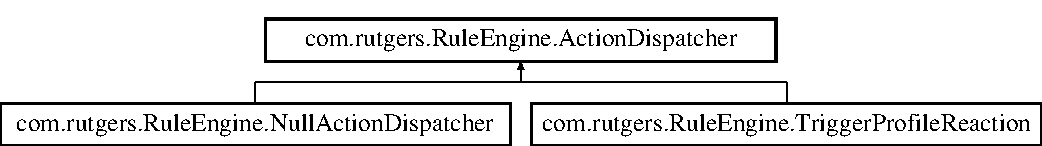
\includegraphics[height=1.958042cm]{interfacecom_1_1rutgers_1_1RuleEngine_1_1ActionDispatcher}
\end{center}
\end{figure}


\subsection{Detailed Description}
\begin{DoxyAuthor}{Author}
eduard 
\end{DoxyAuthor}


The documentation for this interface was generated from the following file\+:\begin{DoxyCompactItemize}
\item 
src/main/java/com/rutgers/\+Rule\+Engine/Action\+Dispatcher.\+java\end{DoxyCompactItemize}

\hypertarget{classcom_1_1rutgers_1_1Android_1_1AndroidPush}{}\section{com.\+rutgers.\+Android.\+Android\+Push Class Reference}
\label{classcom_1_1rutgers_1_1Android_1_1AndroidPush}\index{com.\+rutgers.\+Android.\+Android\+Push@{com.\+rutgers.\+Android.\+Android\+Push}}


\subsection{Detailed Description}
\begin{DoxyAuthor}{Author}
eduard 
\end{DoxyAuthor}


The documentation for this class was generated from the following file\+:\begin{DoxyCompactItemize}
\item 
src/main/java/com/rutgers/\+Android/Android\+Push.\+java\end{DoxyCompactItemize}

\hypertarget{classcom_1_1rutgers_1_1Tree_1_1AVLTree}{}\section{com.\+rutgers.\+Tree.\+A\+V\+L\+Tree Class Reference}
\label{classcom_1_1rutgers_1_1Tree_1_1AVLTree}\index{com.\+rutgers.\+Tree.\+A\+V\+L\+Tree@{com.\+rutgers.\+Tree.\+A\+V\+L\+Tree}}
Inheritance diagram for com.\+rutgers.\+Tree.\+A\+V\+L\+Tree\+:\begin{figure}[H]
\begin{center}
\leavevmode
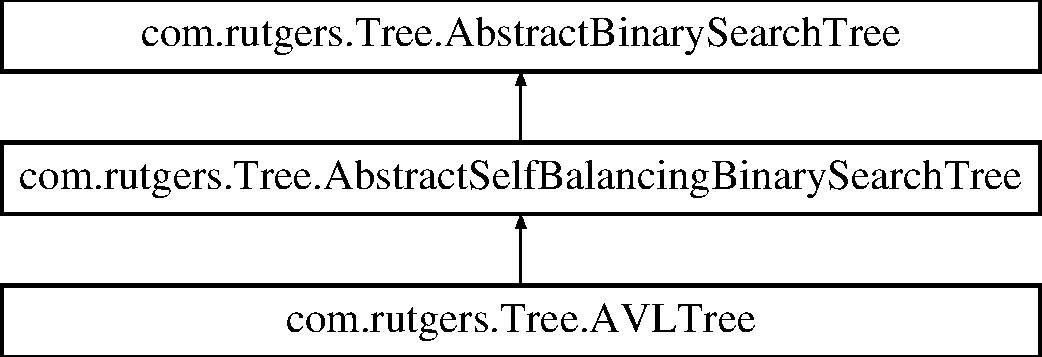
\includegraphics[height=3.000000cm]{classcom_1_1rutgers_1_1Tree_1_1AVLTree}
\end{center}
\end{figure}
\subsection*{Public Member Functions}
\begin{DoxyCompactItemize}
\item 
Node \hyperlink{classcom_1_1rutgers_1_1Tree_1_1AVLTree_a2e0affe74d21a5b18195bac35dde2c06}{insert} (int element)
\end{DoxyCompactItemize}
\subsection*{Protected Member Functions}
\begin{DoxyCompactItemize}
\item 
Node \hyperlink{classcom_1_1rutgers_1_1Tree_1_1AVLTree_a869d4b4c54c71b37d3ac01574f021d90}{double\+Rotate\+Right\+Left} (Node node)
\item 
Node \hyperlink{classcom_1_1rutgers_1_1Tree_1_1AVLTree_a553beb2d927eaca460d22bfa5ce7a337}{double\+Rotate\+Left\+Right} (Node node)
\end{DoxyCompactItemize}
\subsection*{Additional Inherited Members}


\subsection{Detailed Description}
\begin{DoxyAuthor}{Author}
eduard 
\end{DoxyAuthor}


\subsection{Member Function Documentation}
\mbox{\Hypertarget{classcom_1_1rutgers_1_1Tree_1_1AVLTree_a553beb2d927eaca460d22bfa5ce7a337}\label{classcom_1_1rutgers_1_1Tree_1_1AVLTree_a553beb2d927eaca460d22bfa5ce7a337}} 
\index{com\+::rutgers\+::\+Tree\+::\+A\+V\+L\+Tree@{com\+::rutgers\+::\+Tree\+::\+A\+V\+L\+Tree}!double\+Rotate\+Left\+Right@{double\+Rotate\+Left\+Right}}
\index{double\+Rotate\+Left\+Right@{double\+Rotate\+Left\+Right}!com\+::rutgers\+::\+Tree\+::\+A\+V\+L\+Tree@{com\+::rutgers\+::\+Tree\+::\+A\+V\+L\+Tree}}
\subsubsection{\texorpdfstring{double\+Rotate\+Left\+Right()}{doubleRotateLeftRight()}}
{\footnotesize\ttfamily Node com.\+rutgers.\+Tree.\+A\+V\+L\+Tree.\+double\+Rotate\+Left\+Right (\begin{DoxyParamCaption}\item[{Node}]{node }\end{DoxyParamCaption})\hspace{0.3cm}{\ttfamily [protected]}}

Take right child and rotate it to the right side first and then rotate node to the left side. \mbox{\Hypertarget{classcom_1_1rutgers_1_1Tree_1_1AVLTree_a869d4b4c54c71b37d3ac01574f021d90}\label{classcom_1_1rutgers_1_1Tree_1_1AVLTree_a869d4b4c54c71b37d3ac01574f021d90}} 
\index{com\+::rutgers\+::\+Tree\+::\+A\+V\+L\+Tree@{com\+::rutgers\+::\+Tree\+::\+A\+V\+L\+Tree}!double\+Rotate\+Right\+Left@{double\+Rotate\+Right\+Left}}
\index{double\+Rotate\+Right\+Left@{double\+Rotate\+Right\+Left}!com\+::rutgers\+::\+Tree\+::\+A\+V\+L\+Tree@{com\+::rutgers\+::\+Tree\+::\+A\+V\+L\+Tree}}
\subsubsection{\texorpdfstring{double\+Rotate\+Right\+Left()}{doubleRotateRightLeft()}}
{\footnotesize\ttfamily Node com.\+rutgers.\+Tree.\+A\+V\+L\+Tree.\+double\+Rotate\+Right\+Left (\begin{DoxyParamCaption}\item[{Node}]{node }\end{DoxyParamCaption})\hspace{0.3cm}{\ttfamily [protected]}}

Take right child and rotate it to the right side first and then rotate node to the left side. \mbox{\Hypertarget{classcom_1_1rutgers_1_1Tree_1_1AVLTree_a2e0affe74d21a5b18195bac35dde2c06}\label{classcom_1_1rutgers_1_1Tree_1_1AVLTree_a2e0affe74d21a5b18195bac35dde2c06}} 
\index{com\+::rutgers\+::\+Tree\+::\+A\+V\+L\+Tree@{com\+::rutgers\+::\+Tree\+::\+A\+V\+L\+Tree}!insert@{insert}}
\index{insert@{insert}!com\+::rutgers\+::\+Tree\+::\+A\+V\+L\+Tree@{com\+::rutgers\+::\+Tree\+::\+A\+V\+L\+Tree}}
\subsubsection{\texorpdfstring{insert()}{insert()}}
{\footnotesize\ttfamily Node com.\+rutgers.\+Tree.\+A\+V\+L\+Tree.\+insert (\begin{DoxyParamCaption}\item[{int}]{element }\end{DoxyParamCaption})}

\begin{DoxySeeAlso}{See also}
org.\+intelligentjava.\+algos.\+trees.\+Abstract\+Binary\+Search\+Tree\+::insert(int) \begin{DoxyVerb} AVL tree insert method also balances tree if needed. Additional
 height parameter on node is used to track if one subtree is higher
 than other by more than one, if so AVL tree rotations is performed
 to regain balance of the tree.\end{DoxyVerb}
 
\end{DoxySeeAlso}


The documentation for this class was generated from the following file\+:\begin{DoxyCompactItemize}
\item 
src/main/java/com/rutgers/\+Tree/A\+V\+L\+Tree.\+java\end{DoxyCompactItemize}

\hypertarget{classcom_1_1rutgers_1_1Hilbert_1_1Base39}{}\section{com.\+rutgers.\+Hilbert.\+Base39 Class Reference}
\label{classcom_1_1rutgers_1_1Hilbert_1_1Base39}\index{com.\+rutgers.\+Hilbert.\+Base39@{com.\+rutgers.\+Hilbert.\+Base39}}
\subsection*{Public Member Functions}
\begin{DoxyCompactItemize}
\item 
String \hyperlink{classcom_1_1rutgers_1_1Hilbert_1_1Base39_a042a8fe52c1e68fcbde5bcb10f9cae5e}{encode\+Base10} (long b10)
\end{DoxyCompactItemize}
\subsection*{Static Public Member Functions}
\begin{DoxyCompactItemize}
\item 
static long \hyperlink{classcom_1_1rutgers_1_1Hilbert_1_1Base39_ad90f8e29d50c7384c1f149e1bd136de1}{decode\+Base39} (String b62)
\end{DoxyCompactItemize}


\subsection{Detailed Description}
This class defined the \hyperlink{classcom_1_1rutgers_1_1Hilbert_1_1Base39}{Base39} encoding.

\begin{DoxyAuthor}{Author}
Eduard Giber Renart 
\end{DoxyAuthor}
\begin{DoxyVersion}{Version}
1.\+0 
\end{DoxyVersion}


\subsection{Member Function Documentation}
\mbox{\Hypertarget{classcom_1_1rutgers_1_1Hilbert_1_1Base39_ad90f8e29d50c7384c1f149e1bd136de1}\label{classcom_1_1rutgers_1_1Hilbert_1_1Base39_ad90f8e29d50c7384c1f149e1bd136de1}} 
\index{com\+::rutgers\+::\+Hilbert\+::\+Base39@{com\+::rutgers\+::\+Hilbert\+::\+Base39}!decode\+Base39@{decode\+Base39}}
\index{decode\+Base39@{decode\+Base39}!com\+::rutgers\+::\+Hilbert\+::\+Base39@{com\+::rutgers\+::\+Hilbert\+::\+Base39}}
\subsubsection{\texorpdfstring{decode\+Base39()}{decodeBase39()}}
{\footnotesize\ttfamily static long com.\+rutgers.\+Hilbert.\+Base39.\+decode\+Base39 (\begin{DoxyParamCaption}\item[{String}]{b62 }\end{DoxyParamCaption})\hspace{0.3cm}{\ttfamily [static]}}

Decodes a \hyperlink{classcom_1_1rutgers_1_1Hilbert_1_1Base39}{Base39} {\ttfamily String} returning a {\ttfamily long}.


\begin{DoxyParams}{Parameters}
{\em b62} & the \hyperlink{classcom_1_1rutgers_1_1Hilbert_1_1Base39}{Base39} {\ttfamily String} to decode. \\
\hline
\end{DoxyParams}
\begin{DoxyReturn}{Returns}
the decoded number as a {\ttfamily long}. 
\end{DoxyReturn}

\begin{DoxyExceptions}{Exceptions}
{\em Illegal\+Argument\+Exception} & if the given {\ttfamily String} contains characters not specified in the constructor. \\
\hline
\end{DoxyExceptions}
\mbox{\Hypertarget{classcom_1_1rutgers_1_1Hilbert_1_1Base39_a042a8fe52c1e68fcbde5bcb10f9cae5e}\label{classcom_1_1rutgers_1_1Hilbert_1_1Base39_a042a8fe52c1e68fcbde5bcb10f9cae5e}} 
\index{com\+::rutgers\+::\+Hilbert\+::\+Base39@{com\+::rutgers\+::\+Hilbert\+::\+Base39}!encode\+Base10@{encode\+Base10}}
\index{encode\+Base10@{encode\+Base10}!com\+::rutgers\+::\+Hilbert\+::\+Base39@{com\+::rutgers\+::\+Hilbert\+::\+Base39}}
\subsubsection{\texorpdfstring{encode\+Base10()}{encodeBase10()}}
{\footnotesize\ttfamily String com.\+rutgers.\+Hilbert.\+Base39.\+encode\+Base10 (\begin{DoxyParamCaption}\item[{long}]{b10 }\end{DoxyParamCaption})}

Encodes a decimal value to a \hyperlink{classcom_1_1rutgers_1_1Hilbert_1_1Base39}{Base39} {\ttfamily String}.


\begin{DoxyParams}{Parameters}
{\em b10} & the decimal value to encode, must be nonnegative. \\
\hline
\end{DoxyParams}
\begin{DoxyReturn}{Returns}
the number encoded as a \hyperlink{classcom_1_1rutgers_1_1Hilbert_1_1Base39}{Base39} {\ttfamily String}. 
\end{DoxyReturn}


The documentation for this class was generated from the following file\+:\begin{DoxyCompactItemize}
\item 
src/main/java/com/rutgers/\+Hilbert/Base39.\+java\end{DoxyCompactItemize}

\hypertarget{classcom_1_1rutgers_1_1Core_1_1Cli}{}\section{com.\+rutgers.\+Core.\+Cli Class Reference}
\label{classcom_1_1rutgers_1_1Core_1_1Cli}\index{com.\+rutgers.\+Core.\+Cli@{com.\+rutgers.\+Core.\+Cli}}
\subsection*{Public Member Functions}
\begin{DoxyCompactItemize}
\item 
\hyperlink{classcom_1_1rutgers_1_1Core_1_1Cli_a7ae0ec5565a0f5bf6131451f07328d95}{Cli} (String\mbox{[}$\,$\mbox{]} args)
\item 
void \hyperlink{classcom_1_1rutgers_1_1Core_1_1Cli_aaee909416b9655051fbea7611b41d1d4}{parse} ()
\end{DoxyCompactItemize}


\subsection{Detailed Description}
This class is responsible for all the parameters that need to be passed to run R-\/\+Pulsar. It relays on the Apache Commons C\+LI library for parsing command line options passed to programs.

\begin{DoxyAuthor}{Author}
Eduard Giber Renart 
\end{DoxyAuthor}
\begin{DoxyVersion}{Version}
1.\+0 
\end{DoxyVersion}


\subsection{Constructor \& Destructor Documentation}
\mbox{\Hypertarget{classcom_1_1rutgers_1_1Core_1_1Cli_a7ae0ec5565a0f5bf6131451f07328d95}\label{classcom_1_1rutgers_1_1Core_1_1Cli_a7ae0ec5565a0f5bf6131451f07328d95}} 
\index{com\+::rutgers\+::\+Core\+::\+Cli@{com\+::rutgers\+::\+Core\+::\+Cli}!Cli@{Cli}}
\index{Cli@{Cli}!com\+::rutgers\+::\+Core\+::\+Cli@{com\+::rutgers\+::\+Core\+::\+Cli}}
\subsubsection{\texorpdfstring{Cli()}{Cli()}}
{\footnotesize\ttfamily com.\+rutgers.\+Core.\+Cli.\+Cli (\begin{DoxyParamCaption}\item[{String \mbox{[}$\,$\mbox{]}}]{args }\end{DoxyParamCaption})}

This is the main method that is always called when the C\+LI class is instantiated It defines all the parameters that need to be specified in order to run R-\/\+Pulsar. \begin{DoxyReturn}{Returns}
Nothing. 
\end{DoxyReturn}


\subsection{Member Function Documentation}
\mbox{\Hypertarget{classcom_1_1rutgers_1_1Core_1_1Cli_aaee909416b9655051fbea7611b41d1d4}\label{classcom_1_1rutgers_1_1Core_1_1Cli_aaee909416b9655051fbea7611b41d1d4}} 
\index{com\+::rutgers\+::\+Core\+::\+Cli@{com\+::rutgers\+::\+Core\+::\+Cli}!parse@{parse}}
\index{parse@{parse}!com\+::rutgers\+::\+Core\+::\+Cli@{com\+::rutgers\+::\+Core\+::\+Cli}}
\subsubsection{\texorpdfstring{parse()}{parse()}}
{\footnotesize\ttfamily void com.\+rutgers.\+Core.\+Cli.\+parse (\begin{DoxyParamCaption}{ }\end{DoxyParamCaption})}

This is method is called to parse all the parameters that the users inputs. \begin{DoxyReturn}{Returns}
Nothing. 
\end{DoxyReturn}


The documentation for this class was generated from the following file\+:\begin{DoxyCompactItemize}
\item 
src/main/java/com/rutgers/\+Core/Cli.\+java\end{DoxyCompactItemize}

\hypertarget{classcom_1_1rutgers_1_1Examples_1_1Consumer}{}\section{com.\+rutgers.\+Examples.\+Consumer Class Reference}
\label{classcom_1_1rutgers_1_1Examples_1_1Consumer}\index{com.\+rutgers.\+Examples.\+Consumer@{com.\+rutgers.\+Examples.\+Consumer}}
\subsection*{Static Public Member Functions}
\begin{DoxyCompactItemize}
\item 
static void \hyperlink{classcom_1_1rutgers_1_1Examples_1_1Consumer_a7b0c49c85b7cb8c93118d01ab990d025}{main} (String\mbox{[}$\,$\mbox{]} args)  throws Unknown\+Host\+Exception, Class\+Not\+Found\+Exception 
\end{DoxyCompactItemize}


\subsection{Detailed Description}
This is and example of the use of the R-\/\+Pulsar A\+PI. This example shows how to build a R-\/\+Pulsar consumer. 
\begin{DoxyParams}{Parameters}
{\em keys} & \\
\hline
\end{DoxyParams}
\begin{DoxyReturn}{Returns}

\end{DoxyReturn}


\subsection{Member Function Documentation}
\mbox{\Hypertarget{classcom_1_1rutgers_1_1Examples_1_1Consumer_a7b0c49c85b7cb8c93118d01ab990d025}\label{classcom_1_1rutgers_1_1Examples_1_1Consumer_a7b0c49c85b7cb8c93118d01ab990d025}} 
\index{com\+::rutgers\+::\+Examples\+::\+Consumer@{com\+::rutgers\+::\+Examples\+::\+Consumer}!main@{main}}
\index{main@{main}!com\+::rutgers\+::\+Examples\+::\+Consumer@{com\+::rutgers\+::\+Examples\+::\+Consumer}}
\subsubsection{\texorpdfstring{main()}{main()}}
{\footnotesize\ttfamily static void com.\+rutgers.\+Examples.\+Consumer.\+main (\begin{DoxyParamCaption}\item[{String \mbox{[}$\,$\mbox{]}}]{args }\end{DoxyParamCaption}) throws Unknown\+Host\+Exception, Class\+Not\+Found\+Exception\hspace{0.3cm}{\ttfamily [static]}}


\begin{DoxyParams}{Parameters}
{\em args} & the command line arguments \\
\hline
\end{DoxyParams}


The documentation for this class was generated from the following file\+:\begin{DoxyCompactItemize}
\item 
src/main/java/com/rutgers/\+Examples/Consumer.\+java\end{DoxyCompactItemize}

\hypertarget{classcom_1_1rutgers_1_1Core_1_1ConsumerReplyHandler}{}\section{com.\+rutgers.\+Core.\+Consumer\+Reply\+Handler Class Reference}
\label{classcom_1_1rutgers_1_1Core_1_1ConsumerReplyHandler}\index{com.\+rutgers.\+Core.\+Consumer\+Reply\+Handler@{com.\+rutgers.\+Core.\+Consumer\+Reply\+Handler}}


Inherits Runnable.

\subsection*{Public Member Functions}
\begin{DoxyCompactItemize}
\item 
\hyperlink{classcom_1_1rutgers_1_1Core_1_1ConsumerReplyHandler_a850dfa544830ff244044c945de580e65}{Consumer\+Reply\+Handler} (Blocking\+Queue$<$ \hyperlink{classcom_1_1rutgers_1_1Core_1_1Pair}{com.\+rutgers.\+Core.\+Pair}$<$ Peer\+Address, A\+R\+Message $>$$>$ queue, Blocking\+Queue$<$ A\+R\+Message $>$ user\+Queue, Blocking\+Queue$<$ A\+R\+Message $>$ poll\+Queue)  throws I\+O\+Exception 
\item 
Boolean \hyperlink{classcom_1_1rutgers_1_1Core_1_1ConsumerReplyHandler_a02a5478d120604f1c5b9ea578c9a5158}{get\+Running} ()
\item 
void \hyperlink{classcom_1_1rutgers_1_1Core_1_1ConsumerReplyHandler_a8a85b5b1100b63a6d713c0bace5086ac}{set\+Running} (Boolean running)
\item 
void \hyperlink{classcom_1_1rutgers_1_1Core_1_1ConsumerReplyHandler_a975390fd28870020fe1ec8a98c539eca}{run} ()
\end{DoxyCompactItemize}


\subsection{Detailed Description}
This class reacts to the messages recived by other peers.

\begin{DoxyAuthor}{Author}
Eduard Giber Renart 
\end{DoxyAuthor}
\begin{DoxyVersion}{Version}
1.\+0 
\end{DoxyVersion}


\subsection{Constructor \& Destructor Documentation}
\mbox{\Hypertarget{classcom_1_1rutgers_1_1Core_1_1ConsumerReplyHandler_a850dfa544830ff244044c945de580e65}\label{classcom_1_1rutgers_1_1Core_1_1ConsumerReplyHandler_a850dfa544830ff244044c945de580e65}} 
\index{com\+::rutgers\+::\+Core\+::\+Consumer\+Reply\+Handler@{com\+::rutgers\+::\+Core\+::\+Consumer\+Reply\+Handler}!Consumer\+Reply\+Handler@{Consumer\+Reply\+Handler}}
\index{Consumer\+Reply\+Handler@{Consumer\+Reply\+Handler}!com\+::rutgers\+::\+Core\+::\+Consumer\+Reply\+Handler@{com\+::rutgers\+::\+Core\+::\+Consumer\+Reply\+Handler}}
\subsubsection{\texorpdfstring{Consumer\+Reply\+Handler()}{ConsumerReplyHandler()}}
{\footnotesize\ttfamily com.\+rutgers.\+Core.\+Consumer\+Reply\+Handler.\+Consumer\+Reply\+Handler (\begin{DoxyParamCaption}\item[{Blocking\+Queue$<$ \hyperlink{classcom_1_1rutgers_1_1Core_1_1Pair}{com.\+rutgers.\+Core.\+Pair}$<$ Peer\+Address, A\+R\+Message $>$$>$}]{queue,  }\item[{Blocking\+Queue$<$ A\+R\+Message $>$}]{user\+Queue,  }\item[{Blocking\+Queue$<$ A\+R\+Message $>$}]{poll\+Queue }\end{DoxyParamCaption}) throws I\+O\+Exception}

This is the main method which instantiates all the necessary components 
\begin{DoxyParams}{Parameters}
{\em args} & The arguments need to follow the C\+LI implementation. \\
\hline
\end{DoxyParams}
\begin{DoxyReturn}{Returns}
Nothing. 
\end{DoxyReturn}


\subsection{Member Function Documentation}
\mbox{\Hypertarget{classcom_1_1rutgers_1_1Core_1_1ConsumerReplyHandler_a02a5478d120604f1c5b9ea578c9a5158}\label{classcom_1_1rutgers_1_1Core_1_1ConsumerReplyHandler_a02a5478d120604f1c5b9ea578c9a5158}} 
\index{com\+::rutgers\+::\+Core\+::\+Consumer\+Reply\+Handler@{com\+::rutgers\+::\+Core\+::\+Consumer\+Reply\+Handler}!get\+Running@{get\+Running}}
\index{get\+Running@{get\+Running}!com\+::rutgers\+::\+Core\+::\+Consumer\+Reply\+Handler@{com\+::rutgers\+::\+Core\+::\+Consumer\+Reply\+Handler}}
\subsubsection{\texorpdfstring{get\+Running()}{getRunning()}}
{\footnotesize\ttfamily Boolean com.\+rutgers.\+Core.\+Consumer\+Reply\+Handler.\+get\+Running (\begin{DoxyParamCaption}{ }\end{DoxyParamCaption})}

This method return if the class is currently running. \begin{DoxyReturn}{Returns}
If the thread is currently running. 
\end{DoxyReturn}
\mbox{\Hypertarget{classcom_1_1rutgers_1_1Core_1_1ConsumerReplyHandler_a975390fd28870020fe1ec8a98c539eca}\label{classcom_1_1rutgers_1_1Core_1_1ConsumerReplyHandler_a975390fd28870020fe1ec8a98c539eca}} 
\index{com\+::rutgers\+::\+Core\+::\+Consumer\+Reply\+Handler@{com\+::rutgers\+::\+Core\+::\+Consumer\+Reply\+Handler}!run@{run}}
\index{run@{run}!com\+::rutgers\+::\+Core\+::\+Consumer\+Reply\+Handler@{com\+::rutgers\+::\+Core\+::\+Consumer\+Reply\+Handler}}
\subsubsection{\texorpdfstring{run()}{run()}}
{\footnotesize\ttfamily void com.\+rutgers.\+Core.\+Consumer\+Reply\+Handler.\+run (\begin{DoxyParamCaption}{ }\end{DoxyParamCaption})}

This is where to thread loops everytime we receive a message. The first set of message types are for the \hyperlink{classcom_1_1rutgers_1_1Core_1_1RP}{RP}\textquotesingle{}s and then the others are used for the peers. Push message to the local queue.

Check in the local database if a similar profile exists if not just store it.

A match exists then notify both peers to start streaming.

Check in the local database if a similar profile exists if not just store it.

A match exists then notify both peers to start streaming.

Delete profile that the peer previously send.

Delete data that peer send.

Save the storm topology for later execusion.

Start the storm topology.

Stop the storm topology.

All the following messages are used by the peers.

New peer added to the network, we need to add it to the quadtree

Send back all the profiles that are currently stored in the \hyperlink{classcom_1_1rutgers_1_1Core_1_1RP}{RP}.

Store data in the local D\+HT.

Stop the peer.

Get data from the D\+HT.

A new region has been created so we need to updated the peers in our network.\mbox{\Hypertarget{classcom_1_1rutgers_1_1Core_1_1ConsumerReplyHandler_a8a85b5b1100b63a6d713c0bace5086ac}\label{classcom_1_1rutgers_1_1Core_1_1ConsumerReplyHandler_a8a85b5b1100b63a6d713c0bace5086ac}} 
\index{com\+::rutgers\+::\+Core\+::\+Consumer\+Reply\+Handler@{com\+::rutgers\+::\+Core\+::\+Consumer\+Reply\+Handler}!set\+Running@{set\+Running}}
\index{set\+Running@{set\+Running}!com\+::rutgers\+::\+Core\+::\+Consumer\+Reply\+Handler@{com\+::rutgers\+::\+Core\+::\+Consumer\+Reply\+Handler}}
\subsubsection{\texorpdfstring{set\+Running()}{setRunning()}}
{\footnotesize\ttfamily void com.\+rutgers.\+Core.\+Consumer\+Reply\+Handler.\+set\+Running (\begin{DoxyParamCaption}\item[{Boolean}]{running }\end{DoxyParamCaption})}

This method is to start or stop the thread. 
\begin{DoxyParams}{Parameters}
{\em running} & set to true or false to start or stop the thread \\
\hline
\end{DoxyParams}


The documentation for this class was generated from the following file\+:\begin{DoxyCompactItemize}
\item 
src/main/java/com/rutgers/\+Core/Consumer\+Reply\+Handler.\+java\end{DoxyCompactItemize}

\hypertarget{classcom_1_1rutgers_1_1Core_1_1Core}{}\section{com.\+rutgers.\+Core.\+Core Class Reference}
\label{classcom_1_1rutgers_1_1Core_1_1Core}\index{com.\+rutgers.\+Core.\+Core@{com.\+rutgers.\+Core.\+Core}}
\subsection*{Static Public Member Functions}
\begin{DoxyCompactItemize}
\item 
static void \hyperlink{classcom_1_1rutgers_1_1Core_1_1Core_a3372560286c744be181d6e2443a0a1c5}{main} (String\mbox{[}$\,$\mbox{]} args)  throws Interrupted\+Exception, I\+O\+Exception, Invalid\+Key\+Spec\+Exception, Class\+Not\+Found\+Exception 
\end{DoxyCompactItemize}


\subsection{Detailed Description}
\begin{DoxyAuthor}{Author}
eduard 
\end{DoxyAuthor}


\subsection{Member Function Documentation}
\mbox{\Hypertarget{classcom_1_1rutgers_1_1Core_1_1Core_a3372560286c744be181d6e2443a0a1c5}\label{classcom_1_1rutgers_1_1Core_1_1Core_a3372560286c744be181d6e2443a0a1c5}} 
\index{com\+::rutgers\+::\+Core\+::\+Core@{com\+::rutgers\+::\+Core\+::\+Core}!main@{main}}
\index{main@{main}!com\+::rutgers\+::\+Core\+::\+Core@{com\+::rutgers\+::\+Core\+::\+Core}}
\subsubsection{\texorpdfstring{main()}{main()}}
{\footnotesize\ttfamily static void com.\+rutgers.\+Core.\+Core.\+main (\begin{DoxyParamCaption}\item[{String \mbox{[}$\,$\mbox{]}}]{args }\end{DoxyParamCaption}) throws Interrupted\+Exception, I\+O\+Exception, Invalid\+Key\+Spec\+Exception, Class\+Not\+Found\+Exception\hspace{0.3cm}{\ttfamily [static]}}

This is the main method which instantiates the R-\/\+Pulsar node 
\begin{DoxyParams}{Parameters}
{\em args} & The arguments need to follow the C\+LI implementation. \\
\hline
\end{DoxyParams}
\begin{DoxyReturn}{Returns}
Nothing. 
\end{DoxyReturn}
Checks if the boot flag in the C\+LI is set to true If set to false will start and R-\/\+Pulsar Master If set the true will start and R-\/\+Pulsar Slave

Start \hyperlink{classcom_1_1rutgers_1_1Core_1_1RP}{RP} slave.

Send A\+R\+\_\+\+H\+E\+L\+LO to the Master \hyperlink{classcom_1_1rutgers_1_1Core_1_1RP}{RP} so he can add us to the list.

Start and R-\/\+Pulsar master.

Check if user specified a replication factor.

Init the quadtree and add yourself into it.

The documentation for this class was generated from the following file\+:\begin{DoxyCompactItemize}
\item 
src/main/java/com/rutgers/\+Core/Core.\+java\end{DoxyCompactItemize}

\hypertarget{classcom_1_1rutgers_1_1Examples_1_1DHTPublisher}{}\section{com.\+rutgers.\+Examples.\+D\+H\+T\+Publisher Class Reference}
\label{classcom_1_1rutgers_1_1Examples_1_1DHTPublisher}\index{com.\+rutgers.\+Examples.\+D\+H\+T\+Publisher@{com.\+rutgers.\+Examples.\+D\+H\+T\+Publisher}}


\subsection{Detailed Description}
This is and example of the use of the R-\/\+Pulsar A\+PI. This example shows how to build a R-\/\+Pulsar D\+HT \hyperlink{classcom_1_1rutgers_1_1Examples_1_1Publisher}{Publisher}. \begin{DoxyAuthor}{Author}
eduard 
\end{DoxyAuthor}


The documentation for this class was generated from the following file\+:\begin{DoxyCompactItemize}
\item 
src/main/java/com/rutgers/\+Examples/D\+H\+T\+Publisher.\+java\end{DoxyCompactItemize}

\hypertarget{classcom_1_1rutgers_1_1Examples_1_1DHTQuery}{}\section{com.\+rutgers.\+Examples.\+D\+H\+T\+Query Class Reference}
\label{classcom_1_1rutgers_1_1Examples_1_1DHTQuery}\index{com.\+rutgers.\+Examples.\+D\+H\+T\+Query@{com.\+rutgers.\+Examples.\+D\+H\+T\+Query}}


\subsection{Detailed Description}
This is and example of the use of the R-\/\+Pulsar A\+PI. This example shows how to perform D\+HT queries. 
\begin{DoxyParams}{Parameters}
{\em keys} & \\
\hline
\end{DoxyParams}
\begin{DoxyReturn}{Returns}

\end{DoxyReturn}


The documentation for this class was generated from the following file\+:\begin{DoxyCompactItemize}
\item 
src/main/java/com/rutgers/\+Examples/D\+H\+T\+Query.\+java\end{DoxyCompactItemize}

\hypertarget{classcom_1_1rutgers_1_1Core_1_1Globals}{}\section{com.\+rutgers.\+Core.\+Globals Class Reference}
\label{classcom_1_1rutgers_1_1Core_1_1Globals}\index{com.\+rutgers.\+Core.\+Globals@{com.\+rutgers.\+Core.\+Globals}}


\subsection{Detailed Description}
This class is contains all the global variables that are used in R-\/\+Pulsar

\begin{DoxyAuthor}{Author}
Eduard Giber Renart 
\end{DoxyAuthor}
\begin{DoxyVersion}{Version}
1.\+0 
\end{DoxyVersion}


The documentation for this class was generated from the following file\+:\begin{DoxyCompactItemize}
\item 
src/main/java/com/rutgers/\+Core/Globals.\+java\end{DoxyCompactItemize}

\hypertarget{classcom_1_1rutgers_1_1Core_1_1HeartBeat}{}\section{com.\+rutgers.\+Core.\+Heart\+Beat Class Reference}
\label{classcom_1_1rutgers_1_1Core_1_1HeartBeat}\index{com.\+rutgers.\+Core.\+Heart\+Beat@{com.\+rutgers.\+Core.\+Heart\+Beat}}


Inherits Runnable.

\subsection*{Public Member Functions}
\begin{DoxyCompactItemize}
\item 
void \hyperlink{classcom_1_1rutgers_1_1Core_1_1HeartBeat_a0d9ca37ab5618b50adbfd7815549579d}{run} ()
\end{DoxyCompactItemize}


\subsection{Detailed Description}
This class implements the heart beat message that is send to all of the \hyperlink{classcom_1_1rutgers_1_1Core_1_1RP}{RP}\textquotesingle{}s to make sure that they are all alive.

\begin{DoxyAuthor}{Author}
Eduard Giber Renart 
\end{DoxyAuthor}
\begin{DoxyVersion}{Version}
1.\+0 
\end{DoxyVersion}


\subsection{Member Function Documentation}
\mbox{\Hypertarget{classcom_1_1rutgers_1_1Core_1_1HeartBeat_a0d9ca37ab5618b50adbfd7815549579d}\label{classcom_1_1rutgers_1_1Core_1_1HeartBeat_a0d9ca37ab5618b50adbfd7815549579d}} 
\index{com\+::rutgers\+::\+Core\+::\+Heart\+Beat@{com\+::rutgers\+::\+Core\+::\+Heart\+Beat}!run@{run}}
\index{run@{run}!com\+::rutgers\+::\+Core\+::\+Heart\+Beat@{com\+::rutgers\+::\+Core\+::\+Heart\+Beat}}
\subsubsection{\texorpdfstring{run()}{run()}}
{\footnotesize\ttfamily void com.\+rutgers.\+Core.\+Heart\+Beat.\+run (\begin{DoxyParamCaption}{ }\end{DoxyParamCaption})}

This runs in a separate thread and sends pings to all of the peers in the list \begin{DoxyReturn}{Returns}
Nothing. 
\end{DoxyReturn}
Iterate through the peer list

Send a ping and get the latency between the two nodes.

Calculate the average latency amongst all the peers in the list.

The documentation for this class was generated from the following file\+:\begin{DoxyCompactItemize}
\item 
src/main/java/com/rutgers/\+Core/Heart\+Beat.\+java\end{DoxyCompactItemize}

\hypertarget{classcom_1_1rutgers_1_1Hilbert_1_1HilbertCurve}{}\section{com.\+rutgers.\+Hilbert.\+Hilbert\+Curve Class Reference}
\label{classcom_1_1rutgers_1_1Hilbert_1_1HilbertCurve}\index{com.\+rutgers.\+Hilbert.\+Hilbert\+Curve@{com.\+rutgers.\+Hilbert.\+Hilbert\+Curve}}
\subsection*{Public Member Functions}
\begin{DoxyCompactItemize}
\item 
Number160 \hyperlink{classcom_1_1rutgers_1_1Hilbert_1_1HilbertCurve_acf26ba609b064facad3b7e74a3958978}{index} (long... \hyperlink{classcom_1_1rutgers_1_1Hilbert_1_1HilbertCurve_ad3b9f221c5c8e9bada057c09ecb4f8cd}{point})
\item 
long \mbox{[}$\,$\mbox{]} \hyperlink{classcom_1_1rutgers_1_1Hilbert_1_1HilbertCurve_ad3b9f221c5c8e9bada057c09ecb4f8cd}{point} (Number160 \hyperlink{classcom_1_1rutgers_1_1Hilbert_1_1HilbertCurve_acf26ba609b064facad3b7e74a3958978}{index})
\item 
long \mbox{[}$\,$\mbox{]} \hyperlink{classcom_1_1rutgers_1_1Hilbert_1_1HilbertCurve_ac7eecda9bbcd50896e9d16d04fcbc936}{point} (long \hyperlink{classcom_1_1rutgers_1_1Hilbert_1_1HilbertCurve_acf26ba609b064facad3b7e74a3958978}{index})
\end{DoxyCompactItemize}
\subsection*{Static Public Member Functions}
\begin{DoxyCompactItemize}
\item 
static Builder \hyperlink{classcom_1_1rutgers_1_1Hilbert_1_1HilbertCurve_a4393620f0fcf8591df040ceaeb55e756}{bits} (int bits)
\end{DoxyCompactItemize}


\subsection{Detailed Description}
Converts between Hilbert index (
\begin{DoxyCode}
BigInteger 
\end{DoxyCode}
 ) and N-\/dimensional points.

\begin{DoxyAuthor}{Author}
Eduard Giber Renart 
\end{DoxyAuthor}
\begin{DoxyVersion}{Version}
1.\+0 
\end{DoxyVersion}


\subsection{Member Function Documentation}
\mbox{\Hypertarget{classcom_1_1rutgers_1_1Hilbert_1_1HilbertCurve_a4393620f0fcf8591df040ceaeb55e756}\label{classcom_1_1rutgers_1_1Hilbert_1_1HilbertCurve_a4393620f0fcf8591df040ceaeb55e756}} 
\index{com\+::rutgers\+::\+Hilbert\+::\+Hilbert\+Curve@{com\+::rutgers\+::\+Hilbert\+::\+Hilbert\+Curve}!bits@{bits}}
\index{bits@{bits}!com\+::rutgers\+::\+Hilbert\+::\+Hilbert\+Curve@{com\+::rutgers\+::\+Hilbert\+::\+Hilbert\+Curve}}
\subsubsection{\texorpdfstring{bits()}{bits()}}
{\footnotesize\ttfamily static Builder com.\+rutgers.\+Hilbert.\+Hilbert\+Curve.\+bits (\begin{DoxyParamCaption}\item[{int}]{bits }\end{DoxyParamCaption})\hspace{0.3cm}{\ttfamily [static]}}

Returns a builder for and object that performs transformations for a Hilbert curve with the given number of bits.


\begin{DoxyParams}{Parameters}
{\em bits} & depth of the Hilbert curve. If bits is one, this is the top-\/level Hilbert curve \\
\hline
\end{DoxyParams}
\begin{DoxyReturn}{Returns}
builder for object to do transformations with the Hilbert Curve 
\end{DoxyReturn}
\mbox{\Hypertarget{classcom_1_1rutgers_1_1Hilbert_1_1HilbertCurve_acf26ba609b064facad3b7e74a3958978}\label{classcom_1_1rutgers_1_1Hilbert_1_1HilbertCurve_acf26ba609b064facad3b7e74a3958978}} 
\index{com\+::rutgers\+::\+Hilbert\+::\+Hilbert\+Curve@{com\+::rutgers\+::\+Hilbert\+::\+Hilbert\+Curve}!index@{index}}
\index{index@{index}!com\+::rutgers\+::\+Hilbert\+::\+Hilbert\+Curve@{com\+::rutgers\+::\+Hilbert\+::\+Hilbert\+Curve}}
\subsubsection{\texorpdfstring{index()}{index()}}
{\footnotesize\ttfamily Number160 com.\+rutgers.\+Hilbert.\+Hilbert\+Curve.\+index (\begin{DoxyParamCaption}\item[{long...}]{point }\end{DoxyParamCaption})}

Converts a point to its Hilbert curve index.


\begin{DoxyParams}{Parameters}
{\em point} & an array of
\begin{DoxyCode}
\textcolor{keywordtype}{long} 
\end{DoxyCode}
 . Each coordinate can be between 0 and 2\textsuperscript{bits}-\/1. \\
\hline
\end{DoxyParams}
\begin{DoxyReturn}{Returns}
index (nonnegative \hyperlink{}{Big\+Integer}) 
\end{DoxyReturn}

\begin{DoxyExceptions}{Exceptions}
{\em Illegal\+Argument\+Exception} & if length of point array is not equal to the number of dimensions. \\
\hline
\end{DoxyExceptions}
\mbox{\Hypertarget{classcom_1_1rutgers_1_1Hilbert_1_1HilbertCurve_ad3b9f221c5c8e9bada057c09ecb4f8cd}\label{classcom_1_1rutgers_1_1Hilbert_1_1HilbertCurve_ad3b9f221c5c8e9bada057c09ecb4f8cd}} 
\index{com\+::rutgers\+::\+Hilbert\+::\+Hilbert\+Curve@{com\+::rutgers\+::\+Hilbert\+::\+Hilbert\+Curve}!point@{point}}
\index{point@{point}!com\+::rutgers\+::\+Hilbert\+::\+Hilbert\+Curve@{com\+::rutgers\+::\+Hilbert\+::\+Hilbert\+Curve}}
\subsubsection{\texorpdfstring{point()}{point()}\hspace{0.1cm}{\footnotesize\ttfamily [1/2]}}
{\footnotesize\ttfamily long \mbox{[}$\,$\mbox{]} com.\+rutgers.\+Hilbert.\+Hilbert\+Curve.\+point (\begin{DoxyParamCaption}\item[{Number160}]{index }\end{DoxyParamCaption})}

Converts a \hyperlink{}{Big\+Integer} index (distance along the Hilbert Curve from 0) to a point of dimensions defined in the constructor of 
\begin{DoxyCode}
\textcolor{keyword}{this} 
\end{DoxyCode}
 .


\begin{DoxyParams}{Parameters}
{\em index} & index along the Hilbert Curve from 0. Maximum value 2 \textsuperscript{bits $\ast$ dimensions}-\/1. \\
\hline
\end{DoxyParams}
\begin{DoxyReturn}{Returns}
array of longs being the point 
\end{DoxyReturn}

\begin{DoxyExceptions}{Exceptions}
{\em Null\+Pointer\+Exception} & if index is null \\
\hline
{\em Illegal\+Argument\+Exception} & if index is negative \\
\hline
\end{DoxyExceptions}
\mbox{\Hypertarget{classcom_1_1rutgers_1_1Hilbert_1_1HilbertCurve_ac7eecda9bbcd50896e9d16d04fcbc936}\label{classcom_1_1rutgers_1_1Hilbert_1_1HilbertCurve_ac7eecda9bbcd50896e9d16d04fcbc936}} 
\index{com\+::rutgers\+::\+Hilbert\+::\+Hilbert\+Curve@{com\+::rutgers\+::\+Hilbert\+::\+Hilbert\+Curve}!point@{point}}
\index{point@{point}!com\+::rutgers\+::\+Hilbert\+::\+Hilbert\+Curve@{com\+::rutgers\+::\+Hilbert\+::\+Hilbert\+Curve}}
\subsubsection{\texorpdfstring{point()}{point()}\hspace{0.1cm}{\footnotesize\ttfamily [2/2]}}
{\footnotesize\ttfamily long \mbox{[}$\,$\mbox{]} com.\+rutgers.\+Hilbert.\+Hilbert\+Curve.\+point (\begin{DoxyParamCaption}\item[{long}]{index }\end{DoxyParamCaption})}

Converts a
\begin{DoxyCode}
\textcolor{keywordtype}{long} 
\end{DoxyCode}
 index (distance along the Hilbert Curve from 0) to a point of dimensions defined in the constructor of
\begin{DoxyCode}
\textcolor{keyword}{this} 
\end{DoxyCode}
 .


\begin{DoxyParams}{Parameters}
{\em index} & index along the Hilbert Curve from 0. Maximum value 2 \textsuperscript{bits+1}-\/1. \\
\hline
\end{DoxyParams}
\begin{DoxyReturn}{Returns}
array of longs being the point 
\end{DoxyReturn}

\begin{DoxyExceptions}{Exceptions}
{\em Illegal\+Argument\+Exception} & if index is negative \\
\hline
\end{DoxyExceptions}


The documentation for this class was generated from the following file\+:\begin{DoxyCompactItemize}
\item 
src/main/java/com/rutgers/\+Hilbert/Hilbert\+Curve.\+java\end{DoxyCompactItemize}

\hypertarget{classcom_1_1rutgers_1_1Hilbert_1_1HilbertCurveRenderer}{}\section{com.\+rutgers.\+Hilbert.\+Hilbert\+Curve\+Renderer Class Reference}
\label{classcom_1_1rutgers_1_1Hilbert_1_1HilbertCurveRenderer}\index{com.\+rutgers.\+Hilbert.\+Hilbert\+Curve\+Renderer@{com.\+rutgers.\+Hilbert.\+Hilbert\+Curve\+Renderer}}


\subsection{Detailed Description}
This class is used to render a png of the space filling curve. This class is not used in R-\/\+Pulsar is only used for debug. 
\begin{DoxyParams}{Parameters}
{\em keys} & \\
\hline
\end{DoxyParams}
\begin{DoxyReturn}{Returns}

\end{DoxyReturn}


The documentation for this class was generated from the following file\+:\begin{DoxyCompactItemize}
\item 
src/main/java/com/rutgers/\+Hilbert/Hilbert\+Curve\+Renderer.\+java\end{DoxyCompactItemize}

\hypertarget{interfacecom_1_1rutgers_1_1Core_1_1Listener}{}\section{com.\+rutgers.\+Core.\+Listener Interface Reference}
\label{interfacecom_1_1rutgers_1_1Core_1_1Listener}\index{com.\+rutgers.\+Core.\+Listener@{com.\+rutgers.\+Core.\+Listener}}
\subsection*{Public Member Functions}
\begin{DoxyCompactItemize}
\item 
void \hyperlink{interfacecom_1_1rutgers_1_1Core_1_1Listener_a55c7d023e5fcfe48e12986a476410fe7}{replay} (\hyperlink{classcom_1_1rutgers_1_1Core_1_1MessageListener}{Message\+Listener} o, Message.\+A\+R\+Message arg)  throws T\+Exception
\end{DoxyCompactItemize}


\subsection{Detailed Description}
This class is the interface for the message listener.

\begin{DoxyAuthor}{Author}
Eduard Giber Renart 
\end{DoxyAuthor}
\begin{DoxyVersion}{Version}
1.\+0 
\end{DoxyVersion}


\subsection{Member Function Documentation}
\mbox{\Hypertarget{interfacecom_1_1rutgers_1_1Core_1_1Listener_a55c7d023e5fcfe48e12986a476410fe7}\label{interfacecom_1_1rutgers_1_1Core_1_1Listener_a55c7d023e5fcfe48e12986a476410fe7}} 
\index{com\+::rutgers\+::\+Core\+::\+Listener@{com\+::rutgers\+::\+Core\+::\+Listener}!replay@{replay}}
\index{replay@{replay}!com\+::rutgers\+::\+Core\+::\+Listener@{com\+::rutgers\+::\+Core\+::\+Listener}}
\subsubsection{\texorpdfstring{replay()}{replay()}}
{\footnotesize\ttfamily void com.\+rutgers.\+Core.\+Listener.\+replay (\begin{DoxyParamCaption}\item[{\hyperlink{classcom_1_1rutgers_1_1Core_1_1MessageListener}{Message\+Listener}}]{o,  }\item[{Message.\+A\+R\+Message}]{arg }\end{DoxyParamCaption}) throws T\+Exception}

This method is called whenever the observed object is changed. An application calls an {\ttfamily Observable} object\textquotesingle{}s {\ttfamily notify\+Observers} method to have all the object\textquotesingle{}s observers notified of the change.


\begin{DoxyParams}{Parameters}
{\em o} & the observable object. \\
\hline
{\em arg} & an argument passed to the {\ttfamily notify\+Observers} method. \\
\hline
\end{DoxyParams}

\begin{DoxyExceptions}{Exceptions}
{\em T\+Exception} & \\
\hline
\end{DoxyExceptions}


The documentation for this interface was generated from the following file\+:\begin{DoxyCompactItemize}
\item 
src/main/java/com/rutgers/\+Core/Listener.\+java\end{DoxyCompactItemize}

\hypertarget{classcom_1_1rutgers_1_1Core_1_1LocationKeyManager}{}\section{com.\+rutgers.\+Core.\+Location\+Key\+Manager Class Reference}
\label{classcom_1_1rutgers_1_1Core_1_1LocationKeyManager}\index{com.\+rutgers.\+Core.\+Location\+Key\+Manager@{com.\+rutgers.\+Core.\+Location\+Key\+Manager}}
\subsection*{Public Member Functions}
\begin{DoxyCompactItemize}
\item 
\hyperlink{classcom_1_1rutgers_1_1Core_1_1LocationKeyManager_a5b4af0b9881a71b555537e891e27417b}{Location\+Key\+Manager} ()
\item 
synchronized void \hyperlink{classcom_1_1rutgers_1_1Core_1_1LocationKeyManager_ab2468229db734743232c1495d57f418e}{insert\+Key} (Number160 location\+Key, Peer\+Address peer)
\item 
synchronized void \hyperlink{classcom_1_1rutgers_1_1Core_1_1LocationKeyManager_ad824786bd65744f1cb5eca627c4a7fe4}{remove\+Key} (Number160 location\+Key)
\item 
synchronized Peer\+Address \hyperlink{classcom_1_1rutgers_1_1Core_1_1LocationKeyManager_a228d1932314bbf29b6480ffc6eff2ae6}{nearest\+Key} (Number160 location\+Key)
\item 
synchronized Peer\+Address \hyperlink{classcom_1_1rutgers_1_1Core_1_1LocationKeyManager_ae177e62fd90497f20e2c068e236cf95d}{exact\+Key} (Number160 location\+Key)
\item 
synchronized Array\+List$<$ Peer\+Address $>$ \hyperlink{classcom_1_1rutgers_1_1Core_1_1LocationKeyManager_aee8ab17dac0b5ee588ffb29230c7a460}{nearest\+Key} (Number160... location\+Key)
\item 
synchronized Tree\+Map$<$ Number160, Peer\+Address $>$ \hyperlink{classcom_1_1rutgers_1_1Core_1_1LocationKeyManager_a89b55277112464fcb2d6c46e414e09ed}{get\+Cache} ()
\end{DoxyCompactItemize}


\subsection{Detailed Description}
This class is used to find the peers that will be responsible for each data content. Peers are represented as an ID in the form of Number160.

\begin{DoxyAuthor}{Author}
Eduard Giber Renart 
\end{DoxyAuthor}
\begin{DoxyVersion}{Version}
1.\+0 
\end{DoxyVersion}


\subsection{Constructor \& Destructor Documentation}
\mbox{\Hypertarget{classcom_1_1rutgers_1_1Core_1_1LocationKeyManager_a5b4af0b9881a71b555537e891e27417b}\label{classcom_1_1rutgers_1_1Core_1_1LocationKeyManager_a5b4af0b9881a71b555537e891e27417b}} 
\index{com\+::rutgers\+::\+Core\+::\+Location\+Key\+Manager@{com\+::rutgers\+::\+Core\+::\+Location\+Key\+Manager}!Location\+Key\+Manager@{Location\+Key\+Manager}}
\index{Location\+Key\+Manager@{Location\+Key\+Manager}!com\+::rutgers\+::\+Core\+::\+Location\+Key\+Manager@{com\+::rutgers\+::\+Core\+::\+Location\+Key\+Manager}}
\subsubsection{\texorpdfstring{Location\+Key\+Manager()}{LocationKeyManager()}}
{\footnotesize\ttfamily com.\+rutgers.\+Core.\+Location\+Key\+Manager.\+Location\+Key\+Manager (\begin{DoxyParamCaption}{ }\end{DoxyParamCaption})}

Inits the threemap that keeps track if the Number160 and the Peer\+Adress. 

\subsection{Member Function Documentation}
\mbox{\Hypertarget{classcom_1_1rutgers_1_1Core_1_1LocationKeyManager_ae177e62fd90497f20e2c068e236cf95d}\label{classcom_1_1rutgers_1_1Core_1_1LocationKeyManager_ae177e62fd90497f20e2c068e236cf95d}} 
\index{com\+::rutgers\+::\+Core\+::\+Location\+Key\+Manager@{com\+::rutgers\+::\+Core\+::\+Location\+Key\+Manager}!exact\+Key@{exact\+Key}}
\index{exact\+Key@{exact\+Key}!com\+::rutgers\+::\+Core\+::\+Location\+Key\+Manager@{com\+::rutgers\+::\+Core\+::\+Location\+Key\+Manager}}
\subsubsection{\texorpdfstring{exact\+Key()}{exactKey()}}
{\footnotesize\ttfamily synchronized Peer\+Address com.\+rutgers.\+Core.\+Location\+Key\+Manager.\+exact\+Key (\begin{DoxyParamCaption}\item[{Number160}]{location\+Key }\end{DoxyParamCaption})}

Check if we have and exeact location key match. 
\begin{DoxyParams}{Parameters}
{\em location\+Key} & \\
\hline
\end{DoxyParams}
\begin{DoxyReturn}{Returns}
The peer address of the match if exisits. 
\end{DoxyReturn}
\mbox{\Hypertarget{classcom_1_1rutgers_1_1Core_1_1LocationKeyManager_a89b55277112464fcb2d6c46e414e09ed}\label{classcom_1_1rutgers_1_1Core_1_1LocationKeyManager_a89b55277112464fcb2d6c46e414e09ed}} 
\index{com\+::rutgers\+::\+Core\+::\+Location\+Key\+Manager@{com\+::rutgers\+::\+Core\+::\+Location\+Key\+Manager}!get\+Cache@{get\+Cache}}
\index{get\+Cache@{get\+Cache}!com\+::rutgers\+::\+Core\+::\+Location\+Key\+Manager@{com\+::rutgers\+::\+Core\+::\+Location\+Key\+Manager}}
\subsubsection{\texorpdfstring{get\+Cache()}{getCache()}}
{\footnotesize\ttfamily synchronized Tree\+Map$<$Number160, Peer\+Address$>$ com.\+rutgers.\+Core.\+Location\+Key\+Manager.\+get\+Cache (\begin{DoxyParamCaption}{ }\end{DoxyParamCaption})}

Return the treee map object. \begin{DoxyReturn}{Returns}

\end{DoxyReturn}
\mbox{\Hypertarget{classcom_1_1rutgers_1_1Core_1_1LocationKeyManager_ab2468229db734743232c1495d57f418e}\label{classcom_1_1rutgers_1_1Core_1_1LocationKeyManager_ab2468229db734743232c1495d57f418e}} 
\index{com\+::rutgers\+::\+Core\+::\+Location\+Key\+Manager@{com\+::rutgers\+::\+Core\+::\+Location\+Key\+Manager}!insert\+Key@{insert\+Key}}
\index{insert\+Key@{insert\+Key}!com\+::rutgers\+::\+Core\+::\+Location\+Key\+Manager@{com\+::rutgers\+::\+Core\+::\+Location\+Key\+Manager}}
\subsubsection{\texorpdfstring{insert\+Key()}{insertKey()}}
{\footnotesize\ttfamily synchronized void com.\+rutgers.\+Core.\+Location\+Key\+Manager.\+insert\+Key (\begin{DoxyParamCaption}\item[{Number160}]{location\+Key,  }\item[{Peer\+Address}]{peer }\end{DoxyParamCaption})}

Add a new key to the tree map. Used once a new peers comes up. 
\begin{DoxyParams}{Parameters}
{\em location\+Key} & of the peer \\
\hline
{\em peer} & The peer\+Address of the peer. \\
\hline
\end{DoxyParams}
\mbox{\Hypertarget{classcom_1_1rutgers_1_1Core_1_1LocationKeyManager_a228d1932314bbf29b6480ffc6eff2ae6}\label{classcom_1_1rutgers_1_1Core_1_1LocationKeyManager_a228d1932314bbf29b6480ffc6eff2ae6}} 
\index{com\+::rutgers\+::\+Core\+::\+Location\+Key\+Manager@{com\+::rutgers\+::\+Core\+::\+Location\+Key\+Manager}!nearest\+Key@{nearest\+Key}}
\index{nearest\+Key@{nearest\+Key}!com\+::rutgers\+::\+Core\+::\+Location\+Key\+Manager@{com\+::rutgers\+::\+Core\+::\+Location\+Key\+Manager}}
\subsubsection{\texorpdfstring{nearest\+Key()}{nearestKey()}\hspace{0.1cm}{\footnotesize\ttfamily [1/2]}}
{\footnotesize\ttfamily synchronized Peer\+Address com.\+rutgers.\+Core.\+Location\+Key\+Manager.\+nearest\+Key (\begin{DoxyParamCaption}\item[{Number160}]{location\+Key }\end{DoxyParamCaption})}

Find the peer that is closest to the location key provided. 
\begin{DoxyParams}{Parameters}
{\em location\+Key} & location key to search \\
\hline
\end{DoxyParams}
\begin{DoxyReturn}{Returns}
The peer that is closer to the location key provided. 
\end{DoxyReturn}
\mbox{\Hypertarget{classcom_1_1rutgers_1_1Core_1_1LocationKeyManager_aee8ab17dac0b5ee588ffb29230c7a460}\label{classcom_1_1rutgers_1_1Core_1_1LocationKeyManager_aee8ab17dac0b5ee588ffb29230c7a460}} 
\index{com\+::rutgers\+::\+Core\+::\+Location\+Key\+Manager@{com\+::rutgers\+::\+Core\+::\+Location\+Key\+Manager}!nearest\+Key@{nearest\+Key}}
\index{nearest\+Key@{nearest\+Key}!com\+::rutgers\+::\+Core\+::\+Location\+Key\+Manager@{com\+::rutgers\+::\+Core\+::\+Location\+Key\+Manager}}
\subsubsection{\texorpdfstring{nearest\+Key()}{nearestKey()}\hspace{0.1cm}{\footnotesize\ttfamily [2/2]}}
{\footnotesize\ttfamily synchronized Array\+List$<$Peer\+Address$>$ com.\+rutgers.\+Core.\+Location\+Key\+Manager.\+nearest\+Key (\begin{DoxyParamCaption}\item[{Number160...}]{location\+Key }\end{DoxyParamCaption})}

Same method as nearest\+Key the only difference this supports n location keys. 
\begin{DoxyParams}{Parameters}
{\em location\+Key} & Can pass up to n location keys at once. \\
\hline
\end{DoxyParams}
\begin{DoxyReturn}{Returns}
Can return up to n Peer addresses. 
\end{DoxyReturn}
\mbox{\Hypertarget{classcom_1_1rutgers_1_1Core_1_1LocationKeyManager_ad824786bd65744f1cb5eca627c4a7fe4}\label{classcom_1_1rutgers_1_1Core_1_1LocationKeyManager_ad824786bd65744f1cb5eca627c4a7fe4}} 
\index{com\+::rutgers\+::\+Core\+::\+Location\+Key\+Manager@{com\+::rutgers\+::\+Core\+::\+Location\+Key\+Manager}!remove\+Key@{remove\+Key}}
\index{remove\+Key@{remove\+Key}!com\+::rutgers\+::\+Core\+::\+Location\+Key\+Manager@{com\+::rutgers\+::\+Core\+::\+Location\+Key\+Manager}}
\subsubsection{\texorpdfstring{remove\+Key()}{removeKey()}}
{\footnotesize\ttfamily synchronized void com.\+rutgers.\+Core.\+Location\+Key\+Manager.\+remove\+Key (\begin{DoxyParamCaption}\item[{Number160}]{location\+Key }\end{DoxyParamCaption})}

Delete key from the treemap 
\begin{DoxyParams}{Parameters}
{\em location\+Key} & key to delete. \\
\hline
\end{DoxyParams}


The documentation for this class was generated from the following file\+:\begin{DoxyCompactItemize}
\item 
src/main/java/com/rutgers/\+Core/Location\+Key\+Manager.\+java\end{DoxyCompactItemize}

\hypertarget{classcom_1_1rutgers_1_1Core_1_1Manager}{}\section{com.\+rutgers.\+Core.\+Manager Class Reference}
\label{classcom_1_1rutgers_1_1Core_1_1Manager}\index{com.\+rutgers.\+Core.\+Manager@{com.\+rutgers.\+Core.\+Manager}}
\subsection*{Public Member Functions}
\begin{DoxyCompactItemize}
\item 
void \hyperlink{classcom_1_1rutgers_1_1Core_1_1Manager_adbd253cc2bb0c2b905702bc9b214364e}{set\+Rp\+One} (\hyperlink{classcom_1_1rutgers_1_1Core_1_1RP}{RP} rp)
\item 
\hyperlink{classcom_1_1rutgers_1_1Core_1_1RP}{RP} \hyperlink{classcom_1_1rutgers_1_1Core_1_1Manager_aea68f7e919ad032b36085124e38431d1}{get\+Rp\+One} ()
\item 
synchronized long \hyperlink{classcom_1_1rutgers_1_1Core_1_1Manager_abe5c0bf3e6854ec547c1a022c12837b1}{get\+Latency} ()
\item 
void \hyperlink{classcom_1_1rutgers_1_1Core_1_1Manager_ae4f9a9930d85b52eb2ce3b69d2213d11}{set\+Rocks\+D\+B\+MS} (\hyperlink{classcom_1_1rutgers_1_1DB_1_1RocksDBMS}{Rocks\+D\+B\+MS} dbms)
\item 
\hyperlink{classcom_1_1rutgers_1_1DB_1_1RocksDBMS}{Rocks\+D\+B\+MS} \hyperlink{classcom_1_1rutgers_1_1Core_1_1Manager_a04e680889d4e29de3e18e8fe18f0e99e}{get\+Rocks\+D\+B\+MS} ()
\item 
void \hyperlink{classcom_1_1rutgers_1_1Core_1_1Manager_a4803749462ebf23b95f384bb9215c52c}{set\+Latitude} (double latitude)
\item 
void \hyperlink{classcom_1_1rutgers_1_1Core_1_1Manager_a7e1ca7f9d0791baaf3b2a839dacbdc0e}{set\+Longitude} (double longitude)
\item 
double \hyperlink{classcom_1_1rutgers_1_1Core_1_1Manager_aea86a8ba9d78dc6c6b0f6ed5e862c70d}{get\+Latitude} ()
\item 
double \hyperlink{classcom_1_1rutgers_1_1Core_1_1Manager_aea1529f07fb8579f95b51e9463af525b}{get\+Longitude} ()
\item 
boolean \hyperlink{classcom_1_1rutgers_1_1Core_1_1Manager_a0f6d15208fafb97bf0e93ba3b02650bc}{is\+Master} ()
\item 
void \hyperlink{classcom_1_1rutgers_1_1Core_1_1Manager_ac1a4df15343f09e222e19aecc1a2c6f6}{set\+Master} (boolean master)
\item 
\hyperlink{classcom_1_1rutgers_1_1QuadTree_1_1PointQuadTree}{Point\+Quad\+Tree}$<$ Peer\+Address $>$ \hyperlink{classcom_1_1rutgers_1_1Core_1_1Manager_afdfd0fe7b73ad6e3db515ff370095e20}{getq\+Tree} ()
\item 
void \hyperlink{classcom_1_1rutgers_1_1Core_1_1Manager_ab77114e891d4055addf589da5bd5c089}{setq\+Tree} (\hyperlink{classcom_1_1rutgers_1_1QuadTree_1_1PointQuadTree}{Point\+Quad\+Tree}$<$ Peer\+Address $>$ q\+Tree)
\end{DoxyCompactItemize}
\subsection*{Static Public Member Functions}
\begin{DoxyCompactItemize}
\item 
static \hyperlink{classcom_1_1rutgers_1_1Core_1_1Manager}{Manager} \hyperlink{classcom_1_1rutgers_1_1Core_1_1Manager_ab0493d895017b9cb16f383a2f9915a78}{get\+Instance} ()  throws I\+O\+Exception 
\end{DoxyCompactItemize}


\subsection{Detailed Description}
This class is singelton class that will store values and parameters that will be need it at runtime. This class is only instantated once.

\begin{DoxyAuthor}{Author}
Eduard Giber Renart 
\end{DoxyAuthor}
\begin{DoxyVersion}{Version}
1.\+0 
\end{DoxyVersion}


\subsection{Member Function Documentation}
\mbox{\Hypertarget{classcom_1_1rutgers_1_1Core_1_1Manager_ab0493d895017b9cb16f383a2f9915a78}\label{classcom_1_1rutgers_1_1Core_1_1Manager_ab0493d895017b9cb16f383a2f9915a78}} 
\index{com\+::rutgers\+::\+Core\+::\+Manager@{com\+::rutgers\+::\+Core\+::\+Manager}!get\+Instance@{get\+Instance}}
\index{get\+Instance@{get\+Instance}!com\+::rutgers\+::\+Core\+::\+Manager@{com\+::rutgers\+::\+Core\+::\+Manager}}
\subsubsection{\texorpdfstring{get\+Instance()}{getInstance()}}
{\footnotesize\ttfamily static \hyperlink{classcom_1_1rutgers_1_1Core_1_1Manager}{Manager} com.\+rutgers.\+Core.\+Manager.\+get\+Instance (\begin{DoxyParamCaption}{ }\end{DoxyParamCaption}) throws I\+O\+Exception\hspace{0.3cm}{\ttfamily [static]}}

Creates the singelton class \begin{DoxyReturn}{Returns}

\end{DoxyReturn}

\begin{DoxyExceptions}{Exceptions}
{\em I\+O\+Exception} & \\
\hline
\end{DoxyExceptions}
\mbox{\Hypertarget{classcom_1_1rutgers_1_1Core_1_1Manager_abe5c0bf3e6854ec547c1a022c12837b1}\label{classcom_1_1rutgers_1_1Core_1_1Manager_abe5c0bf3e6854ec547c1a022c12837b1}} 
\index{com\+::rutgers\+::\+Core\+::\+Manager@{com\+::rutgers\+::\+Core\+::\+Manager}!get\+Latency@{get\+Latency}}
\index{get\+Latency@{get\+Latency}!com\+::rutgers\+::\+Core\+::\+Manager@{com\+::rutgers\+::\+Core\+::\+Manager}}
\subsubsection{\texorpdfstring{get\+Latency()}{getLatency()}}
{\footnotesize\ttfamily synchronized long com.\+rutgers.\+Core.\+Manager.\+get\+Latency (\begin{DoxyParamCaption}{ }\end{DoxyParamCaption})}

Get the current latency amongst all the \hyperlink{classcom_1_1rutgers_1_1Core_1_1RP}{RP}\textquotesingle{}s. \begin{DoxyReturn}{Returns}

\end{DoxyReturn}
\mbox{\Hypertarget{classcom_1_1rutgers_1_1Core_1_1Manager_aea86a8ba9d78dc6c6b0f6ed5e862c70d}\label{classcom_1_1rutgers_1_1Core_1_1Manager_aea86a8ba9d78dc6c6b0f6ed5e862c70d}} 
\index{com\+::rutgers\+::\+Core\+::\+Manager@{com\+::rutgers\+::\+Core\+::\+Manager}!get\+Latitude@{get\+Latitude}}
\index{get\+Latitude@{get\+Latitude}!com\+::rutgers\+::\+Core\+::\+Manager@{com\+::rutgers\+::\+Core\+::\+Manager}}
\subsubsection{\texorpdfstring{get\+Latitude()}{getLatitude()}}
{\footnotesize\ttfamily double com.\+rutgers.\+Core.\+Manager.\+get\+Latitude (\begin{DoxyParamCaption}{ }\end{DoxyParamCaption})}

Get the current latitude of the \hyperlink{classcom_1_1rutgers_1_1Core_1_1RP}{RP}. \begin{DoxyReturn}{Returns}
latitude 
\end{DoxyReturn}
\mbox{\Hypertarget{classcom_1_1rutgers_1_1Core_1_1Manager_aea1529f07fb8579f95b51e9463af525b}\label{classcom_1_1rutgers_1_1Core_1_1Manager_aea1529f07fb8579f95b51e9463af525b}} 
\index{com\+::rutgers\+::\+Core\+::\+Manager@{com\+::rutgers\+::\+Core\+::\+Manager}!get\+Longitude@{get\+Longitude}}
\index{get\+Longitude@{get\+Longitude}!com\+::rutgers\+::\+Core\+::\+Manager@{com\+::rutgers\+::\+Core\+::\+Manager}}
\subsubsection{\texorpdfstring{get\+Longitude()}{getLongitude()}}
{\footnotesize\ttfamily double com.\+rutgers.\+Core.\+Manager.\+get\+Longitude (\begin{DoxyParamCaption}{ }\end{DoxyParamCaption})}

Get the current longitude of the \hyperlink{classcom_1_1rutgers_1_1Core_1_1RP}{RP}. \begin{DoxyReturn}{Returns}
longitude 
\end{DoxyReturn}
\mbox{\Hypertarget{classcom_1_1rutgers_1_1Core_1_1Manager_afdfd0fe7b73ad6e3db515ff370095e20}\label{classcom_1_1rutgers_1_1Core_1_1Manager_afdfd0fe7b73ad6e3db515ff370095e20}} 
\index{com\+::rutgers\+::\+Core\+::\+Manager@{com\+::rutgers\+::\+Core\+::\+Manager}!getq\+Tree@{getq\+Tree}}
\index{getq\+Tree@{getq\+Tree}!com\+::rutgers\+::\+Core\+::\+Manager@{com\+::rutgers\+::\+Core\+::\+Manager}}
\subsubsection{\texorpdfstring{getq\+Tree()}{getqTree()}}
{\footnotesize\ttfamily \hyperlink{classcom_1_1rutgers_1_1QuadTree_1_1PointQuadTree}{Point\+Quad\+Tree}$<$Peer\+Address$>$ com.\+rutgers.\+Core.\+Manager.\+getq\+Tree (\begin{DoxyParamCaption}{ }\end{DoxyParamCaption})}

Get the quadtree object. \begin{DoxyReturn}{Returns}

\end{DoxyReturn}
\mbox{\Hypertarget{classcom_1_1rutgers_1_1Core_1_1Manager_a04e680889d4e29de3e18e8fe18f0e99e}\label{classcom_1_1rutgers_1_1Core_1_1Manager_a04e680889d4e29de3e18e8fe18f0e99e}} 
\index{com\+::rutgers\+::\+Core\+::\+Manager@{com\+::rutgers\+::\+Core\+::\+Manager}!get\+Rocks\+D\+B\+MS@{get\+Rocks\+D\+B\+MS}}
\index{get\+Rocks\+D\+B\+MS@{get\+Rocks\+D\+B\+MS}!com\+::rutgers\+::\+Core\+::\+Manager@{com\+::rutgers\+::\+Core\+::\+Manager}}
\subsubsection{\texorpdfstring{get\+Rocks\+D\+B\+M\+S()}{getRocksDBMS()}}
{\footnotesize\ttfamily \hyperlink{classcom_1_1rutgers_1_1DB_1_1RocksDBMS}{Rocks\+D\+B\+MS} com.\+rutgers.\+Core.\+Manager.\+get\+Rocks\+D\+B\+MS (\begin{DoxyParamCaption}{ }\end{DoxyParamCaption})}

Get the instance of the Rock D\+B\+MS \begin{DoxyReturn}{Returns}

\end{DoxyReturn}
\mbox{\Hypertarget{classcom_1_1rutgers_1_1Core_1_1Manager_aea68f7e919ad032b36085124e38431d1}\label{classcom_1_1rutgers_1_1Core_1_1Manager_aea68f7e919ad032b36085124e38431d1}} 
\index{com\+::rutgers\+::\+Core\+::\+Manager@{com\+::rutgers\+::\+Core\+::\+Manager}!get\+Rp\+One@{get\+Rp\+One}}
\index{get\+Rp\+One@{get\+Rp\+One}!com\+::rutgers\+::\+Core\+::\+Manager@{com\+::rutgers\+::\+Core\+::\+Manager}}
\subsubsection{\texorpdfstring{get\+Rp\+One()}{getRpOne()}}
{\footnotesize\ttfamily \hyperlink{classcom_1_1rutgers_1_1Core_1_1RP}{RP} com.\+rutgers.\+Core.\+Manager.\+get\+Rp\+One (\begin{DoxyParamCaption}{ }\end{DoxyParamCaption})}

Return the value of \hyperlink{classcom_1_1rutgers_1_1Core_1_1RP}{RP} one \begin{DoxyReturn}{Returns}

\end{DoxyReturn}
\mbox{\Hypertarget{classcom_1_1rutgers_1_1Core_1_1Manager_a0f6d15208fafb97bf0e93ba3b02650bc}\label{classcom_1_1rutgers_1_1Core_1_1Manager_a0f6d15208fafb97bf0e93ba3b02650bc}} 
\index{com\+::rutgers\+::\+Core\+::\+Manager@{com\+::rutgers\+::\+Core\+::\+Manager}!is\+Master@{is\+Master}}
\index{is\+Master@{is\+Master}!com\+::rutgers\+::\+Core\+::\+Manager@{com\+::rutgers\+::\+Core\+::\+Manager}}
\subsubsection{\texorpdfstring{is\+Master()}{isMaster()}}
{\footnotesize\ttfamily boolean com.\+rutgers.\+Core.\+Manager.\+is\+Master (\begin{DoxyParamCaption}{ }\end{DoxyParamCaption})}

Check if we are the master or not \begin{DoxyReturn}{Returns}

\end{DoxyReturn}
\mbox{\Hypertarget{classcom_1_1rutgers_1_1Core_1_1Manager_a4803749462ebf23b95f384bb9215c52c}\label{classcom_1_1rutgers_1_1Core_1_1Manager_a4803749462ebf23b95f384bb9215c52c}} 
\index{com\+::rutgers\+::\+Core\+::\+Manager@{com\+::rutgers\+::\+Core\+::\+Manager}!set\+Latitude@{set\+Latitude}}
\index{set\+Latitude@{set\+Latitude}!com\+::rutgers\+::\+Core\+::\+Manager@{com\+::rutgers\+::\+Core\+::\+Manager}}
\subsubsection{\texorpdfstring{set\+Latitude()}{setLatitude()}}
{\footnotesize\ttfamily void com.\+rutgers.\+Core.\+Manager.\+set\+Latitude (\begin{DoxyParamCaption}\item[{double}]{latitude }\end{DoxyParamCaption})}

Set the current latitude of the \hyperlink{classcom_1_1rutgers_1_1Core_1_1RP}{RP}. 
\begin{DoxyParams}{Parameters}
{\em latitude} & \\
\hline
\end{DoxyParams}
\mbox{\Hypertarget{classcom_1_1rutgers_1_1Core_1_1Manager_a7e1ca7f9d0791baaf3b2a839dacbdc0e}\label{classcom_1_1rutgers_1_1Core_1_1Manager_a7e1ca7f9d0791baaf3b2a839dacbdc0e}} 
\index{com\+::rutgers\+::\+Core\+::\+Manager@{com\+::rutgers\+::\+Core\+::\+Manager}!set\+Longitude@{set\+Longitude}}
\index{set\+Longitude@{set\+Longitude}!com\+::rutgers\+::\+Core\+::\+Manager@{com\+::rutgers\+::\+Core\+::\+Manager}}
\subsubsection{\texorpdfstring{set\+Longitude()}{setLongitude()}}
{\footnotesize\ttfamily void com.\+rutgers.\+Core.\+Manager.\+set\+Longitude (\begin{DoxyParamCaption}\item[{double}]{longitude }\end{DoxyParamCaption})}

Set the current longitude of the \hyperlink{classcom_1_1rutgers_1_1Core_1_1RP}{RP} 
\begin{DoxyParams}{Parameters}
{\em longitude} & \\
\hline
\end{DoxyParams}
\mbox{\Hypertarget{classcom_1_1rutgers_1_1Core_1_1Manager_ac1a4df15343f09e222e19aecc1a2c6f6}\label{classcom_1_1rutgers_1_1Core_1_1Manager_ac1a4df15343f09e222e19aecc1a2c6f6}} 
\index{com\+::rutgers\+::\+Core\+::\+Manager@{com\+::rutgers\+::\+Core\+::\+Manager}!set\+Master@{set\+Master}}
\index{set\+Master@{set\+Master}!com\+::rutgers\+::\+Core\+::\+Manager@{com\+::rutgers\+::\+Core\+::\+Manager}}
\subsubsection{\texorpdfstring{set\+Master()}{setMaster()}}
{\footnotesize\ttfamily void com.\+rutgers.\+Core.\+Manager.\+set\+Master (\begin{DoxyParamCaption}\item[{boolean}]{master }\end{DoxyParamCaption})}

Define who will be the master and save it. 
\begin{DoxyParams}{Parameters}
{\em master} & \\
\hline
\end{DoxyParams}
\mbox{\Hypertarget{classcom_1_1rutgers_1_1Core_1_1Manager_ab77114e891d4055addf589da5bd5c089}\label{classcom_1_1rutgers_1_1Core_1_1Manager_ab77114e891d4055addf589da5bd5c089}} 
\index{com\+::rutgers\+::\+Core\+::\+Manager@{com\+::rutgers\+::\+Core\+::\+Manager}!setq\+Tree@{setq\+Tree}}
\index{setq\+Tree@{setq\+Tree}!com\+::rutgers\+::\+Core\+::\+Manager@{com\+::rutgers\+::\+Core\+::\+Manager}}
\subsubsection{\texorpdfstring{setq\+Tree()}{setqTree()}}
{\footnotesize\ttfamily void com.\+rutgers.\+Core.\+Manager.\+setq\+Tree (\begin{DoxyParamCaption}\item[{\hyperlink{classcom_1_1rutgers_1_1QuadTree_1_1PointQuadTree}{Point\+Quad\+Tree}$<$ Peer\+Address $>$}]{q\+Tree }\end{DoxyParamCaption})}

Set the quadtree object. 
\begin{DoxyParams}{Parameters}
{\em q\+Tree} & \\
\hline
\end{DoxyParams}
\mbox{\Hypertarget{classcom_1_1rutgers_1_1Core_1_1Manager_ae4f9a9930d85b52eb2ce3b69d2213d11}\label{classcom_1_1rutgers_1_1Core_1_1Manager_ae4f9a9930d85b52eb2ce3b69d2213d11}} 
\index{com\+::rutgers\+::\+Core\+::\+Manager@{com\+::rutgers\+::\+Core\+::\+Manager}!set\+Rocks\+D\+B\+MS@{set\+Rocks\+D\+B\+MS}}
\index{set\+Rocks\+D\+B\+MS@{set\+Rocks\+D\+B\+MS}!com\+::rutgers\+::\+Core\+::\+Manager@{com\+::rutgers\+::\+Core\+::\+Manager}}
\subsubsection{\texorpdfstring{set\+Rocks\+D\+B\+M\+S()}{setRocksDBMS()}}
{\footnotesize\ttfamily void com.\+rutgers.\+Core.\+Manager.\+set\+Rocks\+D\+B\+MS (\begin{DoxyParamCaption}\item[{\hyperlink{classcom_1_1rutgers_1_1DB_1_1RocksDBMS}{Rocks\+D\+B\+MS}}]{dbms }\end{DoxyParamCaption})}

Set the instance of the Rock D\+B\+MS 
\begin{DoxyParams}{Parameters}
{\em dbms} & \\
\hline
\end{DoxyParams}
\mbox{\Hypertarget{classcom_1_1rutgers_1_1Core_1_1Manager_adbd253cc2bb0c2b905702bc9b214364e}\label{classcom_1_1rutgers_1_1Core_1_1Manager_adbd253cc2bb0c2b905702bc9b214364e}} 
\index{com\+::rutgers\+::\+Core\+::\+Manager@{com\+::rutgers\+::\+Core\+::\+Manager}!set\+Rp\+One@{set\+Rp\+One}}
\index{set\+Rp\+One@{set\+Rp\+One}!com\+::rutgers\+::\+Core\+::\+Manager@{com\+::rutgers\+::\+Core\+::\+Manager}}
\subsubsection{\texorpdfstring{set\+Rp\+One()}{setRpOne()}}
{\footnotesize\ttfamily void com.\+rutgers.\+Core.\+Manager.\+set\+Rp\+One (\begin{DoxyParamCaption}\item[{\hyperlink{classcom_1_1rutgers_1_1Core_1_1RP}{RP}}]{rp }\end{DoxyParamCaption})}

Set Rp one 
\begin{DoxyParams}{Parameters}
{\em rp} & \\
\hline
\end{DoxyParams}


The documentation for this class was generated from the following file\+:\begin{DoxyCompactItemize}
\item 
src/main/java/com/rutgers/\+Core/Manager.\+java\end{DoxyCompactItemize}

\hypertarget{classcom_1_1rutgers_1_1Core_1_1Message}{}\section{com.\+rutgers.\+Core.\+Message Class Reference}
\label{classcom_1_1rutgers_1_1Core_1_1Message}\index{com.\+rutgers.\+Core.\+Message@{com.\+rutgers.\+Core.\+Message}}


\subsection{Detailed Description}
This class is automatically generated by proto buffer and it contains the structure of the AR message.

\begin{DoxyAuthor}{Author}
Eduard Giber Renart 
\end{DoxyAuthor}
\begin{DoxyVersion}{Version}
1.\+0 
\end{DoxyVersion}


The documentation for this class was generated from the following file\+:\begin{DoxyCompactItemize}
\item 
src/main/java/com/rutgers/\+Core/Message.\+java\end{DoxyCompactItemize}

\hypertarget{classcom_1_1rutgers_1_1Core_1_1MessageListener}{}\section{com.\+rutgers.\+Core.\+Message\+Listener Class Reference}
\label{classcom_1_1rutgers_1_1Core_1_1MessageListener}\index{com.\+rutgers.\+Core.\+Message\+Listener@{com.\+rutgers.\+Core.\+Message\+Listener}}
Inheritance diagram for com.\+rutgers.\+Core.\+Message\+Listener\+:\begin{figure}[H]
\begin{center}
\leavevmode
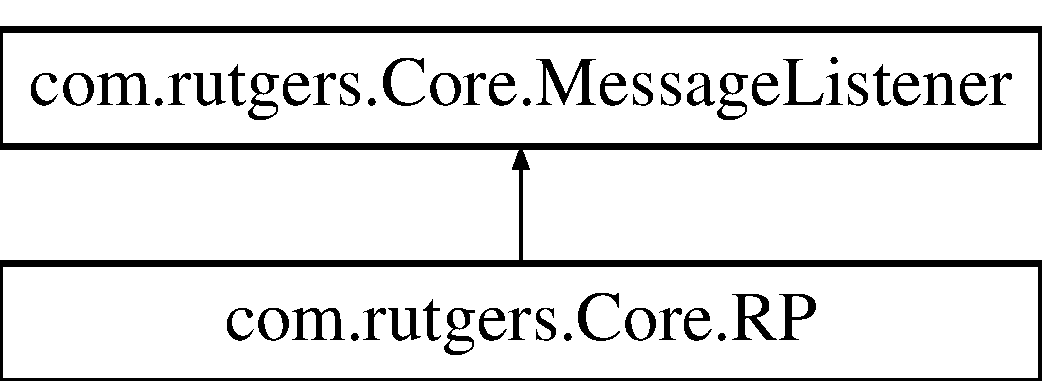
\includegraphics[height=2.000000cm]{classcom_1_1rutgers_1_1Core_1_1MessageListener}
\end{center}
\end{figure}
\subsection*{Public Member Functions}
\begin{DoxyCompactItemize}
\item 
\hyperlink{classcom_1_1rutgers_1_1Core_1_1MessageListener_a62c2c226668ee66cb62b0f9c0070fe17}{Message\+Listener} ()
\item 
synchronized void \hyperlink{classcom_1_1rutgers_1_1Core_1_1MessageListener_a36123785cf1a468272d74d7a394779eb}{add\+Message\+Listener} (\hyperlink{interfacecom_1_1rutgers_1_1Core_1_1Listener}{Listener} o)
\item 
synchronized void \hyperlink{classcom_1_1rutgers_1_1Core_1_1MessageListener_a58dde408a2879983fe3f1a16b7430a2e}{delete\+Message\+Listener} (\hyperlink{interfacecom_1_1rutgers_1_1Core_1_1Listener}{Listener} o)
\item 
void \hyperlink{classcom_1_1rutgers_1_1Core_1_1MessageListener_a2da962a5db69e62ea529759b9f643851}{notify\+Users} ()
\item 
void \hyperlink{classcom_1_1rutgers_1_1Core_1_1MessageListener_a30277268e1459416379eefa0955db46b}{notify\+Users} (Message.\+A\+R\+Message arg)
\item 
synchronized void \hyperlink{classcom_1_1rutgers_1_1Core_1_1MessageListener_abdf30a5ebb8f88e5a0083c9ea0ac48c2}{delete\+Users} ()
\item 
synchronized boolean \hyperlink{classcom_1_1rutgers_1_1Core_1_1MessageListener_a00241c82f572dc5e692a888f450b78d9}{has\+Changed} ()
\item 
synchronized int \hyperlink{classcom_1_1rutgers_1_1Core_1_1MessageListener_a724d20378cbeac3df288bf36622a8bc5}{count\+Observers} ()
\end{DoxyCompactItemize}
\subsection*{Protected Member Functions}
\begin{DoxyCompactItemize}
\item 
synchronized void \hyperlink{classcom_1_1rutgers_1_1Core_1_1MessageListener_a98f9b666ae0b37f818ae53024a10ddad}{set\+Changed} ()
\item 
synchronized void \hyperlink{classcom_1_1rutgers_1_1Core_1_1MessageListener_ad677331c0373ba3a7907119a35ce3a8f}{clear\+Changed} ()
\end{DoxyCompactItemize}


\subsection{Detailed Description}
\begin{DoxyAuthor}{Author}
Eduard Giber Renart 
\end{DoxyAuthor}
\begin{DoxyVersion}{Version}
1.\+0 
\end{DoxyVersion}


\subsection{Constructor \& Destructor Documentation}
\mbox{\Hypertarget{classcom_1_1rutgers_1_1Core_1_1MessageListener_a62c2c226668ee66cb62b0f9c0070fe17}\label{classcom_1_1rutgers_1_1Core_1_1MessageListener_a62c2c226668ee66cb62b0f9c0070fe17}} 
\index{com\+::rutgers\+::\+Core\+::\+Message\+Listener@{com\+::rutgers\+::\+Core\+::\+Message\+Listener}!Message\+Listener@{Message\+Listener}}
\index{Message\+Listener@{Message\+Listener}!com\+::rutgers\+::\+Core\+::\+Message\+Listener@{com\+::rutgers\+::\+Core\+::\+Message\+Listener}}
\subsubsection{\texorpdfstring{Message\+Listener()}{MessageListener()}}
{\footnotesize\ttfamily com.\+rutgers.\+Core.\+Message\+Listener.\+Message\+Listener (\begin{DoxyParamCaption}{ }\end{DoxyParamCaption})}

Construct an Observable with zero Observers. 

\subsection{Member Function Documentation}
\mbox{\Hypertarget{classcom_1_1rutgers_1_1Core_1_1MessageListener_a36123785cf1a468272d74d7a394779eb}\label{classcom_1_1rutgers_1_1Core_1_1MessageListener_a36123785cf1a468272d74d7a394779eb}} 
\index{com\+::rutgers\+::\+Core\+::\+Message\+Listener@{com\+::rutgers\+::\+Core\+::\+Message\+Listener}!add\+Message\+Listener@{add\+Message\+Listener}}
\index{add\+Message\+Listener@{add\+Message\+Listener}!com\+::rutgers\+::\+Core\+::\+Message\+Listener@{com\+::rutgers\+::\+Core\+::\+Message\+Listener}}
\subsubsection{\texorpdfstring{add\+Message\+Listener()}{addMessageListener()}}
{\footnotesize\ttfamily synchronized void com.\+rutgers.\+Core.\+Message\+Listener.\+add\+Message\+Listener (\begin{DoxyParamCaption}\item[{\hyperlink{interfacecom_1_1rutgers_1_1Core_1_1Listener}{Listener}}]{o }\end{DoxyParamCaption})}

Adds an observer to the set of observers for this object, provided that it is not the same as some observer already in the set. The order in which notifications will be delivered to multiple observers is not specified. See the class comment.


\begin{DoxyParams}{Parameters}
{\em o} & an observer to be added. \\
\hline
\end{DoxyParams}

\begin{DoxyExceptions}{Exceptions}
{\em Null\+Pointer\+Exception} & if the parameter o is null. \\
\hline
\end{DoxyExceptions}
\mbox{\Hypertarget{classcom_1_1rutgers_1_1Core_1_1MessageListener_ad677331c0373ba3a7907119a35ce3a8f}\label{classcom_1_1rutgers_1_1Core_1_1MessageListener_ad677331c0373ba3a7907119a35ce3a8f}} 
\index{com\+::rutgers\+::\+Core\+::\+Message\+Listener@{com\+::rutgers\+::\+Core\+::\+Message\+Listener}!clear\+Changed@{clear\+Changed}}
\index{clear\+Changed@{clear\+Changed}!com\+::rutgers\+::\+Core\+::\+Message\+Listener@{com\+::rutgers\+::\+Core\+::\+Message\+Listener}}
\subsubsection{\texorpdfstring{clear\+Changed()}{clearChanged()}}
{\footnotesize\ttfamily synchronized void com.\+rutgers.\+Core.\+Message\+Listener.\+clear\+Changed (\begin{DoxyParamCaption}{ }\end{DoxyParamCaption})\hspace{0.3cm}{\ttfamily [protected]}}

Indicates that this object has no longer changed, or that it has already notified all of its observers of its most recent change, so that the {\ttfamily has\+Changed} method will now return {\ttfamily false}. This method is called automatically by the {\ttfamily notify\+Observers} methods.

\begin{DoxySeeAlso}{See also}
java.\+util.\+Observable\+::notify\+Observers() 

java.\+util.\+Observable\+::notify\+Observers(java.\+lang.\+Object) 
\end{DoxySeeAlso}
\mbox{\Hypertarget{classcom_1_1rutgers_1_1Core_1_1MessageListener_a724d20378cbeac3df288bf36622a8bc5}\label{classcom_1_1rutgers_1_1Core_1_1MessageListener_a724d20378cbeac3df288bf36622a8bc5}} 
\index{com\+::rutgers\+::\+Core\+::\+Message\+Listener@{com\+::rutgers\+::\+Core\+::\+Message\+Listener}!count\+Observers@{count\+Observers}}
\index{count\+Observers@{count\+Observers}!com\+::rutgers\+::\+Core\+::\+Message\+Listener@{com\+::rutgers\+::\+Core\+::\+Message\+Listener}}
\subsubsection{\texorpdfstring{count\+Observers()}{countObservers()}}
{\footnotesize\ttfamily synchronized int com.\+rutgers.\+Core.\+Message\+Listener.\+count\+Observers (\begin{DoxyParamCaption}{ }\end{DoxyParamCaption})}

Returns the number of observers of this {\ttfamily Observable} object.

\begin{DoxyReturn}{Returns}
the number of observers of this object. 
\end{DoxyReturn}
\mbox{\Hypertarget{classcom_1_1rutgers_1_1Core_1_1MessageListener_a58dde408a2879983fe3f1a16b7430a2e}\label{classcom_1_1rutgers_1_1Core_1_1MessageListener_a58dde408a2879983fe3f1a16b7430a2e}} 
\index{com\+::rutgers\+::\+Core\+::\+Message\+Listener@{com\+::rutgers\+::\+Core\+::\+Message\+Listener}!delete\+Message\+Listener@{delete\+Message\+Listener}}
\index{delete\+Message\+Listener@{delete\+Message\+Listener}!com\+::rutgers\+::\+Core\+::\+Message\+Listener@{com\+::rutgers\+::\+Core\+::\+Message\+Listener}}
\subsubsection{\texorpdfstring{delete\+Message\+Listener()}{deleteMessageListener()}}
{\footnotesize\ttfamily synchronized void com.\+rutgers.\+Core.\+Message\+Listener.\+delete\+Message\+Listener (\begin{DoxyParamCaption}\item[{\hyperlink{interfacecom_1_1rutgers_1_1Core_1_1Listener}{Listener}}]{o }\end{DoxyParamCaption})}

Deletes an observer from the set of observers of this object. Passing {\ttfamily null} to this method will have no effect. 
\begin{DoxyParams}{Parameters}
{\em o} & the observer to be deleted. \\
\hline
\end{DoxyParams}
\mbox{\Hypertarget{classcom_1_1rutgers_1_1Core_1_1MessageListener_abdf30a5ebb8f88e5a0083c9ea0ac48c2}\label{classcom_1_1rutgers_1_1Core_1_1MessageListener_abdf30a5ebb8f88e5a0083c9ea0ac48c2}} 
\index{com\+::rutgers\+::\+Core\+::\+Message\+Listener@{com\+::rutgers\+::\+Core\+::\+Message\+Listener}!delete\+Users@{delete\+Users}}
\index{delete\+Users@{delete\+Users}!com\+::rutgers\+::\+Core\+::\+Message\+Listener@{com\+::rutgers\+::\+Core\+::\+Message\+Listener}}
\subsubsection{\texorpdfstring{delete\+Users()}{deleteUsers()}}
{\footnotesize\ttfamily synchronized void com.\+rutgers.\+Core.\+Message\+Listener.\+delete\+Users (\begin{DoxyParamCaption}{ }\end{DoxyParamCaption})}

Clears the observer list so that this object no longer has any observers. \mbox{\Hypertarget{classcom_1_1rutgers_1_1Core_1_1MessageListener_a00241c82f572dc5e692a888f450b78d9}\label{classcom_1_1rutgers_1_1Core_1_1MessageListener_a00241c82f572dc5e692a888f450b78d9}} 
\index{com\+::rutgers\+::\+Core\+::\+Message\+Listener@{com\+::rutgers\+::\+Core\+::\+Message\+Listener}!has\+Changed@{has\+Changed}}
\index{has\+Changed@{has\+Changed}!com\+::rutgers\+::\+Core\+::\+Message\+Listener@{com\+::rutgers\+::\+Core\+::\+Message\+Listener}}
\subsubsection{\texorpdfstring{has\+Changed()}{hasChanged()}}
{\footnotesize\ttfamily synchronized boolean com.\+rutgers.\+Core.\+Message\+Listener.\+has\+Changed (\begin{DoxyParamCaption}{ }\end{DoxyParamCaption})}

Tests if this object has changed.

\begin{DoxyReturn}{Returns}
{\ttfamily true} if and only if the {\ttfamily set\+Changed} method has been called more recently than the {\ttfamily clear\+Changed} method on this object; {\ttfamily false} otherwise. 
\end{DoxyReturn}
\begin{DoxySeeAlso}{See also}
java.\+util.\+Observable\+::clear\+Changed() 

java.\+util.\+Observable\+::set\+Changed() 
\end{DoxySeeAlso}
\mbox{\Hypertarget{classcom_1_1rutgers_1_1Core_1_1MessageListener_a2da962a5db69e62ea529759b9f643851}\label{classcom_1_1rutgers_1_1Core_1_1MessageListener_a2da962a5db69e62ea529759b9f643851}} 
\index{com\+::rutgers\+::\+Core\+::\+Message\+Listener@{com\+::rutgers\+::\+Core\+::\+Message\+Listener}!notify\+Users@{notify\+Users}}
\index{notify\+Users@{notify\+Users}!com\+::rutgers\+::\+Core\+::\+Message\+Listener@{com\+::rutgers\+::\+Core\+::\+Message\+Listener}}
\subsubsection{\texorpdfstring{notify\+Users()}{notifyUsers()}\hspace{0.1cm}{\footnotesize\ttfamily [1/2]}}
{\footnotesize\ttfamily void com.\+rutgers.\+Core.\+Message\+Listener.\+notify\+Users (\begin{DoxyParamCaption}{ }\end{DoxyParamCaption})}

If this object has changed, as indicated by the {\ttfamily has\+Changed} method, then notify all of its observers and then call the {\ttfamily clear\+Changed} method to indicate that this object has no longer changed. 

Each observer has its {\ttfamily update} method called with two arguments\+: this observable object and {\ttfamily null}. In other words, this method is equivalent to\+: \begin{quote}
{\ttfamily  notify\+Observers(null)}\end{quote}


\begin{DoxySeeAlso}{See also}
java.\+util.\+Observable\+::clear\+Changed() 

java.\+util.\+Observable\+::has\+Changed() 

java.\+util.\+Observer\+::update(java.\+util.\+Observable, java.\+lang.\+Object) 
\end{DoxySeeAlso}
\mbox{\Hypertarget{classcom_1_1rutgers_1_1Core_1_1MessageListener_a30277268e1459416379eefa0955db46b}\label{classcom_1_1rutgers_1_1Core_1_1MessageListener_a30277268e1459416379eefa0955db46b}} 
\index{com\+::rutgers\+::\+Core\+::\+Message\+Listener@{com\+::rutgers\+::\+Core\+::\+Message\+Listener}!notify\+Users@{notify\+Users}}
\index{notify\+Users@{notify\+Users}!com\+::rutgers\+::\+Core\+::\+Message\+Listener@{com\+::rutgers\+::\+Core\+::\+Message\+Listener}}
\subsubsection{\texorpdfstring{notify\+Users()}{notifyUsers()}\hspace{0.1cm}{\footnotesize\ttfamily [2/2]}}
{\footnotesize\ttfamily void com.\+rutgers.\+Core.\+Message\+Listener.\+notify\+Users (\begin{DoxyParamCaption}\item[{Message.\+A\+R\+Message}]{arg }\end{DoxyParamCaption})}

If this object has changed, as indicated by the {\ttfamily has\+Changed} method, then notify all of its observers and then call the {\ttfamily clear\+Changed} method to indicate that this object has no longer changed. 

Each observer has its {\ttfamily update} method called with two arguments\+: this observable object and the {\ttfamily arg} argument.


\begin{DoxyParams}{Parameters}
{\em arg} & any object. \\
\hline
\end{DoxyParams}
\begin{DoxySeeAlso}{See also}
java.\+util.\+Observable\+::clear\+Changed() 

java.\+util.\+Observable\+::has\+Changed() 

java.\+util.\+Observer\+::update(java.\+util.\+Observable, java.\+lang.\+Object) 
\end{DoxySeeAlso}
\mbox{\Hypertarget{classcom_1_1rutgers_1_1Core_1_1MessageListener_a98f9b666ae0b37f818ae53024a10ddad}\label{classcom_1_1rutgers_1_1Core_1_1MessageListener_a98f9b666ae0b37f818ae53024a10ddad}} 
\index{com\+::rutgers\+::\+Core\+::\+Message\+Listener@{com\+::rutgers\+::\+Core\+::\+Message\+Listener}!set\+Changed@{set\+Changed}}
\index{set\+Changed@{set\+Changed}!com\+::rutgers\+::\+Core\+::\+Message\+Listener@{com\+::rutgers\+::\+Core\+::\+Message\+Listener}}
\subsubsection{\texorpdfstring{set\+Changed()}{setChanged()}}
{\footnotesize\ttfamily synchronized void com.\+rutgers.\+Core.\+Message\+Listener.\+set\+Changed (\begin{DoxyParamCaption}{ }\end{DoxyParamCaption})\hspace{0.3cm}{\ttfamily [protected]}}

Marks this {\ttfamily Observable} object as having been changed; the {\ttfamily has\+Changed} method will now return {\ttfamily true}. 

The documentation for this class was generated from the following file\+:\begin{DoxyCompactItemize}
\item 
src/main/java/com/rutgers/\+Core/Message\+Listener.\+java\end{DoxyCompactItemize}

\hypertarget{classcom_1_1rutgers_1_1RuleEngine_1_1NullActionDispatcher}{}\section{com.\+rutgers.\+Rule\+Engine.\+Null\+Action\+Dispatcher Class Reference}
\label{classcom_1_1rutgers_1_1RuleEngine_1_1NullActionDispatcher}\index{com.\+rutgers.\+Rule\+Engine.\+Null\+Action\+Dispatcher@{com.\+rutgers.\+Rule\+Engine.\+Null\+Action\+Dispatcher}}
Inheritance diagram for com.\+rutgers.\+Rule\+Engine.\+Null\+Action\+Dispatcher\+:\begin{figure}[H]
\begin{center}
\leavevmode
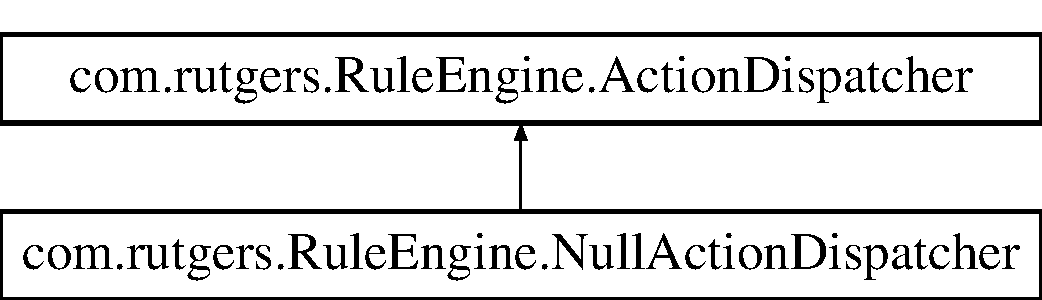
\includegraphics[height=2.000000cm]{classcom_1_1rutgers_1_1RuleEngine_1_1NullActionDispatcher}
\end{center}
\end{figure}


\subsection{Detailed Description}
\begin{DoxyAuthor}{Author}
eduard 
\end{DoxyAuthor}


The documentation for this class was generated from the following file\+:\begin{DoxyCompactItemize}
\item 
src/main/java/com/rutgers/\+Rule\+Engine/Null\+Action\+Dispatcher.\+java\end{DoxyCompactItemize}

\hypertarget{classcom_1_1rutgers_1_1Core_1_1Pair}{}\section{com.\+rutgers.\+Core.\+Pair$<$ K, V $>$ Class Template Reference}
\label{classcom_1_1rutgers_1_1Core_1_1Pair}\index{com.\+rutgers.\+Core.\+Pair$<$ K, V $>$@{com.\+rutgers.\+Core.\+Pair$<$ K, V $>$}}
\subsection*{Public Member Functions}
\begin{DoxyCompactItemize}
\item 
\hyperlink{classcom_1_1rutgers_1_1Core_1_1Pair_a7953f3267ac99110e0e7446d5361cc62}{Pair} (K element0, V element1)
\item 
K \hyperlink{classcom_1_1rutgers_1_1Core_1_1Pair_aa1ee0d8fa231e29cbc7a7d3ad64738c2}{get\+Element0} ()
\item 
V \hyperlink{classcom_1_1rutgers_1_1Core_1_1Pair_a4815bd5515106b5d9fb2113f94b184d2}{get\+Element1} ()
\end{DoxyCompactItemize}


\subsection{Detailed Description}
Implements a \hyperlink{classcom_1_1rutgers_1_1Core_1_1Pair}{Pair} and will be used in R-\/\+Pulsar \begin{DoxyAuthor}{Author}
eduard 
\end{DoxyAuthor}

\begin{DoxyParams}{Parameters}
{\em $<$\+K$>$} & \\
\hline
{\em $<$\+V$>$} & \\
\hline
\end{DoxyParams}


\subsection{Constructor \& Destructor Documentation}
\mbox{\Hypertarget{classcom_1_1rutgers_1_1Core_1_1Pair_a7953f3267ac99110e0e7446d5361cc62}\label{classcom_1_1rutgers_1_1Core_1_1Pair_a7953f3267ac99110e0e7446d5361cc62}} 
\index{com\+::rutgers\+::\+Core\+::\+Pair@{com\+::rutgers\+::\+Core\+::\+Pair}!Pair@{Pair}}
\index{Pair@{Pair}!com\+::rutgers\+::\+Core\+::\+Pair@{com\+::rutgers\+::\+Core\+::\+Pair}}
\subsubsection{\texorpdfstring{Pair()}{Pair()}}
{\footnotesize\ttfamily \hyperlink{classcom_1_1rutgers_1_1Core_1_1Pair}{com.\+rutgers.\+Core.\+Pair}$<$ K, V $>$.\hyperlink{classcom_1_1rutgers_1_1Core_1_1Pair}{Pair} (\begin{DoxyParamCaption}\item[{K}]{element0,  }\item[{V}]{element1 }\end{DoxyParamCaption})}

Create pair and init with the values passed 
\begin{DoxyParams}{Parameters}
{\em element0} & \\
\hline
{\em element1} & \\
\hline
\end{DoxyParams}


\subsection{Member Function Documentation}
\mbox{\Hypertarget{classcom_1_1rutgers_1_1Core_1_1Pair_aa1ee0d8fa231e29cbc7a7d3ad64738c2}\label{classcom_1_1rutgers_1_1Core_1_1Pair_aa1ee0d8fa231e29cbc7a7d3ad64738c2}} 
\index{com\+::rutgers\+::\+Core\+::\+Pair@{com\+::rutgers\+::\+Core\+::\+Pair}!get\+Element0@{get\+Element0}}
\index{get\+Element0@{get\+Element0}!com\+::rutgers\+::\+Core\+::\+Pair@{com\+::rutgers\+::\+Core\+::\+Pair}}
\subsubsection{\texorpdfstring{get\+Element0()}{getElement0()}}
{\footnotesize\ttfamily K \hyperlink{classcom_1_1rutgers_1_1Core_1_1Pair}{com.\+rutgers.\+Core.\+Pair}$<$ K, V $>$.get\+Element0 (\begin{DoxyParamCaption}{ }\end{DoxyParamCaption})}

Get Element0 \begin{DoxyReturn}{Returns}
Will return the element0 in the pair. 
\end{DoxyReturn}
\mbox{\Hypertarget{classcom_1_1rutgers_1_1Core_1_1Pair_a4815bd5515106b5d9fb2113f94b184d2}\label{classcom_1_1rutgers_1_1Core_1_1Pair_a4815bd5515106b5d9fb2113f94b184d2}} 
\index{com\+::rutgers\+::\+Core\+::\+Pair@{com\+::rutgers\+::\+Core\+::\+Pair}!get\+Element1@{get\+Element1}}
\index{get\+Element1@{get\+Element1}!com\+::rutgers\+::\+Core\+::\+Pair@{com\+::rutgers\+::\+Core\+::\+Pair}}
\subsubsection{\texorpdfstring{get\+Element1()}{getElement1()}}
{\footnotesize\ttfamily V \hyperlink{classcom_1_1rutgers_1_1Core_1_1Pair}{com.\+rutgers.\+Core.\+Pair}$<$ K, V $>$.get\+Element1 (\begin{DoxyParamCaption}{ }\end{DoxyParamCaption})}

Get Element1 \begin{DoxyReturn}{Returns}
Will return the element1 in the pair. 
\end{DoxyReturn}


The documentation for this class was generated from the following file\+:\begin{DoxyCompactItemize}
\item 
src/main/java/com/rutgers/\+Core/Pair.\+java\end{DoxyCompactItemize}

\hypertarget{classcom_1_1rutgers_1_1QuadTree_1_1PointNode}{}\section{com.\+rutgers.\+Quad\+Tree.\+Point\+Node$<$ T $>$ Class Template Reference}
\label{classcom_1_1rutgers_1_1QuadTree_1_1PointNode}\index{com.\+rutgers.\+Quad\+Tree.\+Point\+Node$<$ T $>$@{com.\+rutgers.\+Quad\+Tree.\+Point\+Node$<$ T $>$}}
Inheritance diagram for com.\+rutgers.\+Quad\+Tree.\+Point\+Node$<$ T $>$\+:\begin{figure}[H]
\begin{center}
\leavevmode
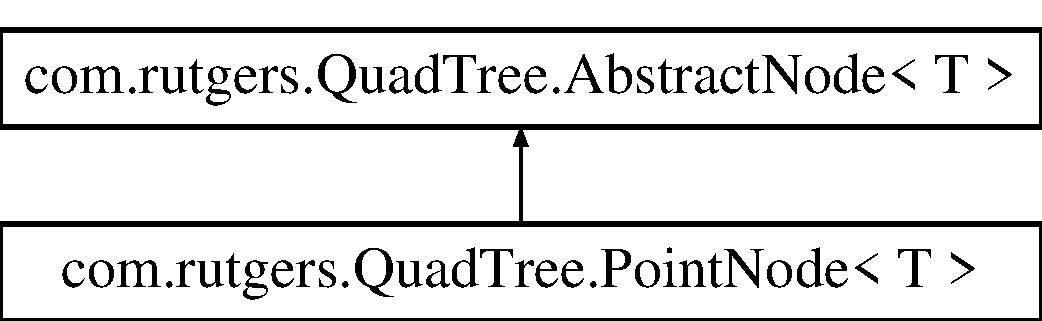
\includegraphics[height=2.000000cm]{classcom_1_1rutgers_1_1QuadTree_1_1PointNode}
\end{center}
\end{figure}
\subsection*{Public Member Functions}
\begin{DoxyCompactItemize}
\item 
\hyperlink{classcom_1_1rutgers_1_1QuadTree_1_1PointNode_a3c57944cb98cfd710608b57fefcd64c2}{Point\+Node} (double north, double south, double east, double west, int depth, int max\+Depth, int max\+Children)
\item 
Map$<$ Cell, \hyperlink{classcom_1_1rutgers_1_1QuadTree_1_1PointNode}{Point\+Node}$<$ T $>$ $>$ \hyperlink{classcom_1_1rutgers_1_1QuadTree_1_1PointNode_a0e45f85c9b62f83648033a73c4d8247a}{get\+Sub\+Nodes} ()
\item 
Vector$<$ \hyperlink{classcom_1_1rutgers_1_1QuadTree_1_1PointNodeElement}{Point\+Node\+Element}$<$ T $>$ $>$ \hyperlink{classcom_1_1rutgers_1_1QuadTree_1_1PointNode_a59932b71d5045e3192a093ed57361140}{get\+Elements} ()
\item 
Vector$<$ \hyperlink{classcom_1_1rutgers_1_1QuadTree_1_1PointNodeElement}{Point\+Node\+Element}$<$ T $>$ $>$ \hyperlink{classcom_1_1rutgers_1_1QuadTree_1_1PointNode_abf17594daa50fa4958b91a2991fcb1a1}{get\+Elements} (double latitude, double longitude)
\item 
void \hyperlink{classcom_1_1rutgers_1_1QuadTree_1_1PointNode_a8b9eceb7216cbb98a251c6fbc3d42d4b}{insert} (\hyperlink{classcom_1_1rutgers_1_1QuadTree_1_1PointNodeElement}{Point\+Node\+Element}$<$ T $>$ element)
\item 
void \hyperlink{classcom_1_1rutgers_1_1QuadTree_1_1PointNode_a0177d4d297bf8a6fdeac5b014f1205df}{subdivide} ()
\item 
boolean \hyperlink{classcom_1_1rutgers_1_1QuadTree_1_1PointNode_ad9eb9b306f9604a2c688a6c906cb6e83}{test\+Subdivide} ()
\item 
void \hyperlink{classcom_1_1rutgers_1_1QuadTree_1_1PointNode_a806f2958ac623cadc0687adc2b7df724}{clear} ()
\end{DoxyCompactItemize}
\subsection*{Protected Member Functions}
\begin{DoxyCompactItemize}
\item 
Cell \hyperlink{classcom_1_1rutgers_1_1QuadTree_1_1PointNode_a6d835e3113b4c96c6300a09dd3702d81}{find\+Index} (double latitude, double longitude)
\end{DoxyCompactItemize}
\subsection*{Protected Attributes}
\begin{DoxyCompactItemize}
\item 
Vector$<$ \hyperlink{classcom_1_1rutgers_1_1QuadTree_1_1PointNodeElement}{Point\+Node\+Element}$<$ T $>$ $>$ \hyperlink{classcom_1_1rutgers_1_1QuadTree_1_1PointNode_a0e05238a78062b65ab3953980cb8889c}{elements} = new Vector$<$\hyperlink{classcom_1_1rutgers_1_1QuadTree_1_1PointNodeElement}{Point\+Node\+Element}$<$T$>$$>$()
\end{DoxyCompactItemize}
\subsection*{Additional Inherited Members}


\subsection{Detailed Description}
This class defines the Point Node.

\begin{DoxyAuthor}{Author}
Eduard Giber Renart 
\end{DoxyAuthor}
\begin{DoxyVersion}{Version}
1.\+0 
\end{DoxyVersion}


\subsection{Constructor \& Destructor Documentation}
\mbox{\Hypertarget{classcom_1_1rutgers_1_1QuadTree_1_1PointNode_a3c57944cb98cfd710608b57fefcd64c2}\label{classcom_1_1rutgers_1_1QuadTree_1_1PointNode_a3c57944cb98cfd710608b57fefcd64c2}} 
\index{com\+::rutgers\+::\+Quad\+Tree\+::\+Point\+Node@{com\+::rutgers\+::\+Quad\+Tree\+::\+Point\+Node}!Point\+Node@{Point\+Node}}
\index{Point\+Node@{Point\+Node}!com\+::rutgers\+::\+Quad\+Tree\+::\+Point\+Node@{com\+::rutgers\+::\+Quad\+Tree\+::\+Point\+Node}}
\subsubsection{\texorpdfstring{Point\+Node()}{PointNode()}}
{\footnotesize\ttfamily \hyperlink{classcom_1_1rutgers_1_1QuadTree_1_1PointNode}{com.\+rutgers.\+Quad\+Tree.\+Point\+Node}$<$ T $>$.\hyperlink{classcom_1_1rutgers_1_1QuadTree_1_1PointNode}{Point\+Node} (\begin{DoxyParamCaption}\item[{double}]{north,  }\item[{double}]{south,  }\item[{double}]{east,  }\item[{double}]{west,  }\item[{int}]{depth,  }\item[{int}]{max\+Depth,  }\item[{int}]{max\+Children }\end{DoxyParamCaption})}


\begin{DoxyParams}{Parameters}
{\em start\+Coordinates} & \\
\hline
{\em bounds} & \\
\hline
{\em depth} & \\
\hline
{\em max\+Depth} & \\
\hline
{\em max\+Children} & \\
\hline
\end{DoxyParams}


\subsection{Member Function Documentation}
\mbox{\Hypertarget{classcom_1_1rutgers_1_1QuadTree_1_1PointNode_a806f2958ac623cadc0687adc2b7df724}\label{classcom_1_1rutgers_1_1QuadTree_1_1PointNode_a806f2958ac623cadc0687adc2b7df724}} 
\index{com\+::rutgers\+::\+Quad\+Tree\+::\+Point\+Node@{com\+::rutgers\+::\+Quad\+Tree\+::\+Point\+Node}!clear@{clear}}
\index{clear@{clear}!com\+::rutgers\+::\+Quad\+Tree\+::\+Point\+Node@{com\+::rutgers\+::\+Quad\+Tree\+::\+Point\+Node}}
\subsubsection{\texorpdfstring{clear()}{clear()}}
{\footnotesize\ttfamily void \hyperlink{classcom_1_1rutgers_1_1QuadTree_1_1PointNode}{com.\+rutgers.\+Quad\+Tree.\+Point\+Node}$<$ T $>$.clear (\begin{DoxyParamCaption}{ }\end{DoxyParamCaption})}

Clears this node and all subnodes \mbox{\Hypertarget{classcom_1_1rutgers_1_1QuadTree_1_1PointNode_a6d835e3113b4c96c6300a09dd3702d81}\label{classcom_1_1rutgers_1_1QuadTree_1_1PointNode_a6d835e3113b4c96c6300a09dd3702d81}} 
\index{com\+::rutgers\+::\+Quad\+Tree\+::\+Point\+Node@{com\+::rutgers\+::\+Quad\+Tree\+::\+Point\+Node}!find\+Index@{find\+Index}}
\index{find\+Index@{find\+Index}!com\+::rutgers\+::\+Quad\+Tree\+::\+Point\+Node@{com\+::rutgers\+::\+Quad\+Tree\+::\+Point\+Node}}
\subsubsection{\texorpdfstring{find\+Index()}{findIndex()}}
{\footnotesize\ttfamily Cell \hyperlink{classcom_1_1rutgers_1_1QuadTree_1_1PointNode}{com.\+rutgers.\+Quad\+Tree.\+Point\+Node}$<$ T $>$.find\+Index (\begin{DoxyParamCaption}\item[{double}]{latitude,  }\item[{double}]{longitude }\end{DoxyParamCaption})\hspace{0.3cm}{\ttfamily [protected]}}

Returns the cell of this element


\begin{DoxyParams}{Parameters}
{\em element} & \\
\hline
\end{DoxyParams}
\begin{DoxyReturn}{Returns}

\end{DoxyReturn}
\mbox{\Hypertarget{classcom_1_1rutgers_1_1QuadTree_1_1PointNode_a59932b71d5045e3192a093ed57361140}\label{classcom_1_1rutgers_1_1QuadTree_1_1PointNode_a59932b71d5045e3192a093ed57361140}} 
\index{com\+::rutgers\+::\+Quad\+Tree\+::\+Point\+Node@{com\+::rutgers\+::\+Quad\+Tree\+::\+Point\+Node}!get\+Elements@{get\+Elements}}
\index{get\+Elements@{get\+Elements}!com\+::rutgers\+::\+Quad\+Tree\+::\+Point\+Node@{com\+::rutgers\+::\+Quad\+Tree\+::\+Point\+Node}}
\subsubsection{\texorpdfstring{get\+Elements()}{getElements()}\hspace{0.1cm}{\footnotesize\ttfamily [1/2]}}
{\footnotesize\ttfamily Vector$<$\hyperlink{classcom_1_1rutgers_1_1QuadTree_1_1PointNodeElement}{Point\+Node\+Element}$<$T$>$ $>$ \hyperlink{classcom_1_1rutgers_1_1QuadTree_1_1PointNode}{com.\+rutgers.\+Quad\+Tree.\+Point\+Node}$<$ T $>$.get\+Elements (\begin{DoxyParamCaption}{ }\end{DoxyParamCaption})}

Returns all elements for this node

\begin{DoxyReturn}{Returns}

\end{DoxyReturn}
\mbox{\Hypertarget{classcom_1_1rutgers_1_1QuadTree_1_1PointNode_abf17594daa50fa4958b91a2991fcb1a1}\label{classcom_1_1rutgers_1_1QuadTree_1_1PointNode_abf17594daa50fa4958b91a2991fcb1a1}} 
\index{com\+::rutgers\+::\+Quad\+Tree\+::\+Point\+Node@{com\+::rutgers\+::\+Quad\+Tree\+::\+Point\+Node}!get\+Elements@{get\+Elements}}
\index{get\+Elements@{get\+Elements}!com\+::rutgers\+::\+Quad\+Tree\+::\+Point\+Node@{com\+::rutgers\+::\+Quad\+Tree\+::\+Point\+Node}}
\subsubsection{\texorpdfstring{get\+Elements()}{getElements()}\hspace{0.1cm}{\footnotesize\ttfamily [2/2]}}
{\footnotesize\ttfamily Vector$<$\hyperlink{classcom_1_1rutgers_1_1QuadTree_1_1PointNodeElement}{Point\+Node\+Element}$<$T$>$ $>$ \hyperlink{classcom_1_1rutgers_1_1QuadTree_1_1PointNode}{com.\+rutgers.\+Quad\+Tree.\+Point\+Node}$<$ T $>$.get\+Elements (\begin{DoxyParamCaption}\item[{double}]{latitude,  }\item[{double}]{longitude }\end{DoxyParamCaption})}

Returns all elements within the cell that matches the given coordinates


\begin{DoxyParams}{Parameters}
{\em coordinates} & \\
\hline
\end{DoxyParams}
\begin{DoxyReturn}{Returns}

\end{DoxyReturn}
\mbox{\Hypertarget{classcom_1_1rutgers_1_1QuadTree_1_1PointNode_a0e45f85c9b62f83648033a73c4d8247a}\label{classcom_1_1rutgers_1_1QuadTree_1_1PointNode_a0e45f85c9b62f83648033a73c4d8247a}} 
\index{com\+::rutgers\+::\+Quad\+Tree\+::\+Point\+Node@{com\+::rutgers\+::\+Quad\+Tree\+::\+Point\+Node}!get\+Sub\+Nodes@{get\+Sub\+Nodes}}
\index{get\+Sub\+Nodes@{get\+Sub\+Nodes}!com\+::rutgers\+::\+Quad\+Tree\+::\+Point\+Node@{com\+::rutgers\+::\+Quad\+Tree\+::\+Point\+Node}}
\subsubsection{\texorpdfstring{get\+Sub\+Nodes()}{getSubNodes()}}
{\footnotesize\ttfamily Map$<$Cell, \hyperlink{classcom_1_1rutgers_1_1QuadTree_1_1PointNode}{Point\+Node}$<$T$>$ $>$ \hyperlink{classcom_1_1rutgers_1_1QuadTree_1_1PointNode}{com.\+rutgers.\+Quad\+Tree.\+Point\+Node}$<$ T $>$.get\+Sub\+Nodes (\begin{DoxyParamCaption}{ }\end{DoxyParamCaption})}

Returns the subnodes of this node

\begin{DoxyReturn}{Returns}

\end{DoxyReturn}
\mbox{\Hypertarget{classcom_1_1rutgers_1_1QuadTree_1_1PointNode_a8b9eceb7216cbb98a251c6fbc3d42d4b}\label{classcom_1_1rutgers_1_1QuadTree_1_1PointNode_a8b9eceb7216cbb98a251c6fbc3d42d4b}} 
\index{com\+::rutgers\+::\+Quad\+Tree\+::\+Point\+Node@{com\+::rutgers\+::\+Quad\+Tree\+::\+Point\+Node}!insert@{insert}}
\index{insert@{insert}!com\+::rutgers\+::\+Quad\+Tree\+::\+Point\+Node@{com\+::rutgers\+::\+Quad\+Tree\+::\+Point\+Node}}
\subsubsection{\texorpdfstring{insert()}{insert()}}
{\footnotesize\ttfamily void \hyperlink{classcom_1_1rutgers_1_1QuadTree_1_1PointNode}{com.\+rutgers.\+Quad\+Tree.\+Point\+Node}$<$ T $>$.insert (\begin{DoxyParamCaption}\item[{\hyperlink{classcom_1_1rutgers_1_1QuadTree_1_1PointNodeElement}{Point\+Node\+Element}$<$ T $>$}]{element }\end{DoxyParamCaption})}

Insert the element into this node. If needed a subdivision will be performed


\begin{DoxyParams}{Parameters}
{\em element} & \\
\hline
\end{DoxyParams}
\mbox{\Hypertarget{classcom_1_1rutgers_1_1QuadTree_1_1PointNode_a0177d4d297bf8a6fdeac5b014f1205df}\label{classcom_1_1rutgers_1_1QuadTree_1_1PointNode_a0177d4d297bf8a6fdeac5b014f1205df}} 
\index{com\+::rutgers\+::\+Quad\+Tree\+::\+Point\+Node@{com\+::rutgers\+::\+Quad\+Tree\+::\+Point\+Node}!subdivide@{subdivide}}
\index{subdivide@{subdivide}!com\+::rutgers\+::\+Quad\+Tree\+::\+Point\+Node@{com\+::rutgers\+::\+Quad\+Tree\+::\+Point\+Node}}
\subsubsection{\texorpdfstring{subdivide()}{subdivide()}}
{\footnotesize\ttfamily void \hyperlink{classcom_1_1rutgers_1_1QuadTree_1_1PointNode}{com.\+rutgers.\+Quad\+Tree.\+Point\+Node}$<$ T $>$.subdivide (\begin{DoxyParamCaption}{ }\end{DoxyParamCaption})}

Subdivide the current node and add subnodes \mbox{\Hypertarget{classcom_1_1rutgers_1_1QuadTree_1_1PointNode_ad9eb9b306f9604a2c688a6c906cb6e83}\label{classcom_1_1rutgers_1_1QuadTree_1_1PointNode_ad9eb9b306f9604a2c688a6c906cb6e83}} 
\index{com\+::rutgers\+::\+Quad\+Tree\+::\+Point\+Node@{com\+::rutgers\+::\+Quad\+Tree\+::\+Point\+Node}!test\+Subdivide@{test\+Subdivide}}
\index{test\+Subdivide@{test\+Subdivide}!com\+::rutgers\+::\+Quad\+Tree\+::\+Point\+Node@{com\+::rutgers\+::\+Quad\+Tree\+::\+Point\+Node}}
\subsubsection{\texorpdfstring{test\+Subdivide()}{testSubdivide()}}
{\footnotesize\ttfamily boolean \hyperlink{classcom_1_1rutgers_1_1QuadTree_1_1PointNode}{com.\+rutgers.\+Quad\+Tree.\+Point\+Node}$<$ T $>$.test\+Subdivide (\begin{DoxyParamCaption}{ }\end{DoxyParamCaption})}

Test if we can subdivide the current node and add subnodes 

\subsection{Member Data Documentation}
\mbox{\Hypertarget{classcom_1_1rutgers_1_1QuadTree_1_1PointNode_a0e05238a78062b65ab3953980cb8889c}\label{classcom_1_1rutgers_1_1QuadTree_1_1PointNode_a0e05238a78062b65ab3953980cb8889c}} 
\index{com\+::rutgers\+::\+Quad\+Tree\+::\+Point\+Node@{com\+::rutgers\+::\+Quad\+Tree\+::\+Point\+Node}!elements@{elements}}
\index{elements@{elements}!com\+::rutgers\+::\+Quad\+Tree\+::\+Point\+Node@{com\+::rutgers\+::\+Quad\+Tree\+::\+Point\+Node}}
\subsubsection{\texorpdfstring{elements}{elements}}
{\footnotesize\ttfamily Vector$<$\hyperlink{classcom_1_1rutgers_1_1QuadTree_1_1PointNodeElement}{Point\+Node\+Element}$<$T$>$ $>$ \hyperlink{classcom_1_1rutgers_1_1QuadTree_1_1PointNode}{com.\+rutgers.\+Quad\+Tree.\+Point\+Node}$<$ T $>$.elements = new Vector$<$\hyperlink{classcom_1_1rutgers_1_1QuadTree_1_1PointNodeElement}{Point\+Node\+Element}$<$T$>$$>$()\hspace{0.3cm}{\ttfamily [protected]}}

Holds all elements for this node 

The documentation for this class was generated from the following file\+:\begin{DoxyCompactItemize}
\item 
src/main/java/com/rutgers/\+Quad\+Tree/Point\+Node.\+java\end{DoxyCompactItemize}

\hypertarget{classcom_1_1rutgers_1_1QuadTree_1_1PointNodeElement}{}\section{com.\+rutgers.\+Quad\+Tree.\+Point\+Node\+Element$<$ T $>$ Class Template Reference}
\label{classcom_1_1rutgers_1_1QuadTree_1_1PointNodeElement}\index{com.\+rutgers.\+Quad\+Tree.\+Point\+Node\+Element$<$ T $>$@{com.\+rutgers.\+Quad\+Tree.\+Point\+Node\+Element$<$ T $>$}}
Inheritance diagram for com.\+rutgers.\+Quad\+Tree.\+Point\+Node\+Element$<$ T $>$\+:\begin{figure}[H]
\begin{center}
\leavevmode
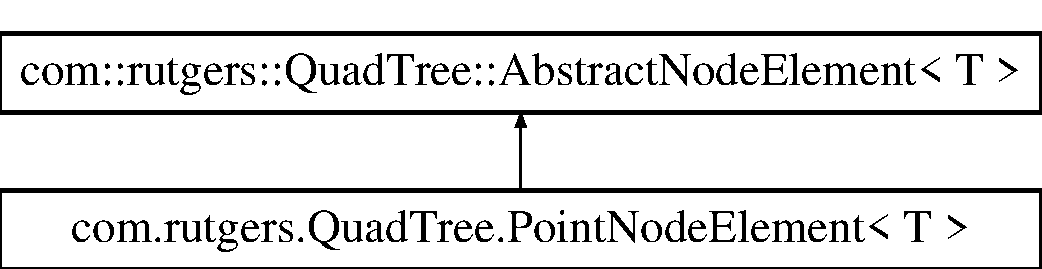
\includegraphics[height=2.000000cm]{classcom_1_1rutgers_1_1QuadTree_1_1PointNodeElement}
\end{center}
\end{figure}
\subsection*{Additional Inherited Members}


\subsection{Detailed Description}
This class defines the Point Node Element.

\begin{DoxyAuthor}{Author}
Eduard Giber Renart 
\end{DoxyAuthor}
\begin{DoxyVersion}{Version}
1.\+0 
\end{DoxyVersion}


The documentation for this class was generated from the following file\+:\begin{DoxyCompactItemize}
\item 
src/main/java/com/rutgers/\+Quad\+Tree/Point\+Node\+Element.\+java\end{DoxyCompactItemize}

\hypertarget{classcom_1_1rutgers_1_1QuadTree_1_1PointQuadTree}{}\section{com.\+rutgers.\+Quad\+Tree.\+Point\+Quad\+Tree$<$ T $>$ Class Template Reference}
\label{classcom_1_1rutgers_1_1QuadTree_1_1PointQuadTree}\index{com.\+rutgers.\+Quad\+Tree.\+Point\+Quad\+Tree$<$ T $>$@{com.\+rutgers.\+Quad\+Tree.\+Point\+Quad\+Tree$<$ T $>$}}
Inheritance diagram for com.\+rutgers.\+Quad\+Tree.\+Point\+Quad\+Tree$<$ T $>$\+:\begin{figure}[H]
\begin{center}
\leavevmode
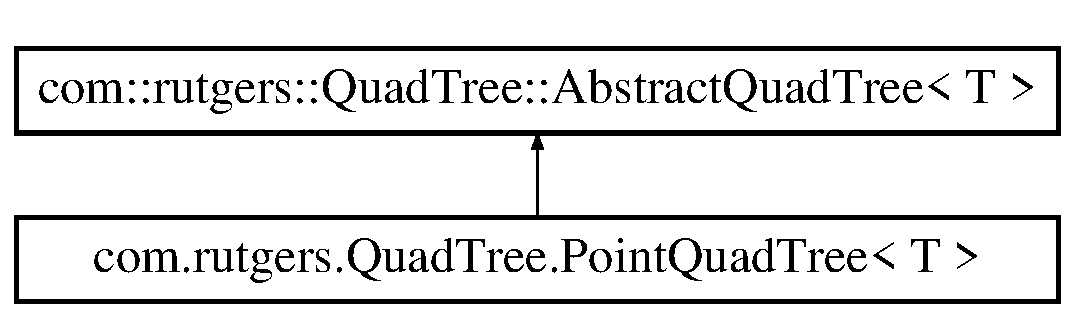
\includegraphics[height=2.000000cm]{classcom_1_1rutgers_1_1QuadTree_1_1PointQuadTree}
\end{center}
\end{figure}
\subsection*{Public Member Functions}
\begin{DoxyCompactItemize}
\item 
\hyperlink{classcom_1_1rutgers_1_1QuadTree_1_1PointQuadTree_a0f0ff8a241617971f6e96d2e2ffe9a1f}{Point\+Quad\+Tree} (double north, double south, double east, double west)  throws I\+O\+Exception 
\item 
void \hyperlink{classcom_1_1rutgers_1_1QuadTree_1_1PointQuadTree_af18b98ffc4fa1a7c2e803db8c8f59392}{insert} (double latitude, double longitude, T element, String icon)  throws No\+Such\+Algorithm\+Exception, Invalid\+Key\+Spec\+Exception 
\item 
\hyperlink{classcom_1_1rutgers_1_1QuadTree_1_1PointNode}{Point\+Node}$<$ T $>$ \hyperlink{classcom_1_1rutgers_1_1QuadTree_1_1PointQuadTree_a7038d1d0c8f55c00b38bbd440c31e9aa}{get\+Root\+Node} ()
\item 
Vector$<$? extends \hyperlink{classcom_1_1rutgers_1_1QuadTree_1_1AbstractNodeElement}{Abstract\+Node\+Element}$<$ T $>$ $>$ \hyperlink{classcom_1_1rutgers_1_1QuadTree_1_1PointQuadTree_a9968a70d79ddfe49dc2dac031389648f}{get\+Elements} (double latitude, double longitude)
\end{DoxyCompactItemize}


\subsection{Detailed Description}
This is the main class of the quadtree

\begin{DoxyAuthor}{Author}
Eduard Giber Renart 
\end{DoxyAuthor}
\begin{DoxyVersion}{Version}
1.\+0 
\end{DoxyVersion}


\subsection{Constructor \& Destructor Documentation}
\mbox{\Hypertarget{classcom_1_1rutgers_1_1QuadTree_1_1PointQuadTree_a0f0ff8a241617971f6e96d2e2ffe9a1f}\label{classcom_1_1rutgers_1_1QuadTree_1_1PointQuadTree_a0f0ff8a241617971f6e96d2e2ffe9a1f}} 
\index{com\+::rutgers\+::\+Quad\+Tree\+::\+Point\+Quad\+Tree@{com\+::rutgers\+::\+Quad\+Tree\+::\+Point\+Quad\+Tree}!Point\+Quad\+Tree@{Point\+Quad\+Tree}}
\index{Point\+Quad\+Tree@{Point\+Quad\+Tree}!com\+::rutgers\+::\+Quad\+Tree\+::\+Point\+Quad\+Tree@{com\+::rutgers\+::\+Quad\+Tree\+::\+Point\+Quad\+Tree}}
\subsubsection{\texorpdfstring{Point\+Quad\+Tree()}{PointQuadTree()}}
{\footnotesize\ttfamily \hyperlink{classcom_1_1rutgers_1_1QuadTree_1_1PointQuadTree}{com.\+rutgers.\+Quad\+Tree.\+Point\+Quad\+Tree}$<$ T $>$.\hyperlink{classcom_1_1rutgers_1_1QuadTree_1_1PointQuadTree}{Point\+Quad\+Tree} (\begin{DoxyParamCaption}\item[{double}]{north,  }\item[{double}]{south,  }\item[{double}]{east,  }\item[{double}]{west }\end{DoxyParamCaption}) throws I\+O\+Exception}

Create a new Quad\+Tree with the give start coordinates and size


\begin{DoxyParams}{Parameters}
{\em start\+Corrdinates} & \\
\hline
{\em size} & \\
\hline
\end{DoxyParams}


\subsection{Member Function Documentation}
\mbox{\Hypertarget{classcom_1_1rutgers_1_1QuadTree_1_1PointQuadTree_a9968a70d79ddfe49dc2dac031389648f}\label{classcom_1_1rutgers_1_1QuadTree_1_1PointQuadTree_a9968a70d79ddfe49dc2dac031389648f}} 
\index{com\+::rutgers\+::\+Quad\+Tree\+::\+Point\+Quad\+Tree@{com\+::rutgers\+::\+Quad\+Tree\+::\+Point\+Quad\+Tree}!get\+Elements@{get\+Elements}}
\index{get\+Elements@{get\+Elements}!com\+::rutgers\+::\+Quad\+Tree\+::\+Point\+Quad\+Tree@{com\+::rutgers\+::\+Quad\+Tree\+::\+Point\+Quad\+Tree}}
\subsubsection{\texorpdfstring{get\+Elements()}{getElements()}}
{\footnotesize\ttfamily Vector$<$? extends \hyperlink{classcom_1_1rutgers_1_1QuadTree_1_1AbstractNodeElement}{Abstract\+Node\+Element}$<$T$>$ $>$ \hyperlink{classcom_1_1rutgers_1_1QuadTree_1_1PointQuadTree}{com.\+rutgers.\+Quad\+Tree.\+Point\+Quad\+Tree}$<$ T $>$.get\+Elements (\begin{DoxyParamCaption}\item[{double}]{latitude,  }\item[{double}]{longitude }\end{DoxyParamCaption})}

Returns all elements wihtin the cell that matches the given coordinates


\begin{DoxyParams}{Parameters}
{\em coordinates} & \\
\hline
\end{DoxyParams}
\begin{DoxyReturn}{Returns}

\end{DoxyReturn}
\mbox{\Hypertarget{classcom_1_1rutgers_1_1QuadTree_1_1PointQuadTree_a7038d1d0c8f55c00b38bbd440c31e9aa}\label{classcom_1_1rutgers_1_1QuadTree_1_1PointQuadTree_a7038d1d0c8f55c00b38bbd440c31e9aa}} 
\index{com\+::rutgers\+::\+Quad\+Tree\+::\+Point\+Quad\+Tree@{com\+::rutgers\+::\+Quad\+Tree\+::\+Point\+Quad\+Tree}!get\+Root\+Node@{get\+Root\+Node}}
\index{get\+Root\+Node@{get\+Root\+Node}!com\+::rutgers\+::\+Quad\+Tree\+::\+Point\+Quad\+Tree@{com\+::rutgers\+::\+Quad\+Tree\+::\+Point\+Quad\+Tree}}
\subsubsection{\texorpdfstring{get\+Root\+Node()}{getRootNode()}}
{\footnotesize\ttfamily \hyperlink{classcom_1_1rutgers_1_1QuadTree_1_1PointNode}{Point\+Node}$<$T$>$ \hyperlink{classcom_1_1rutgers_1_1QuadTree_1_1PointQuadTree}{com.\+rutgers.\+Quad\+Tree.\+Point\+Quad\+Tree}$<$ T $>$.get\+Root\+Node (\begin{DoxyParamCaption}{ }\end{DoxyParamCaption})}

Returns the root\+Node of this tree

\begin{DoxyReturn}{Returns}

\end{DoxyReturn}
\mbox{\Hypertarget{classcom_1_1rutgers_1_1QuadTree_1_1PointQuadTree_af18b98ffc4fa1a7c2e803db8c8f59392}\label{classcom_1_1rutgers_1_1QuadTree_1_1PointQuadTree_af18b98ffc4fa1a7c2e803db8c8f59392}} 
\index{com\+::rutgers\+::\+Quad\+Tree\+::\+Point\+Quad\+Tree@{com\+::rutgers\+::\+Quad\+Tree\+::\+Point\+Quad\+Tree}!insert@{insert}}
\index{insert@{insert}!com\+::rutgers\+::\+Quad\+Tree\+::\+Point\+Quad\+Tree@{com\+::rutgers\+::\+Quad\+Tree\+::\+Point\+Quad\+Tree}}
\subsubsection{\texorpdfstring{insert()}{insert()}}
{\footnotesize\ttfamily void \hyperlink{classcom_1_1rutgers_1_1QuadTree_1_1PointQuadTree}{com.\+rutgers.\+Quad\+Tree.\+Point\+Quad\+Tree}$<$ T $>$.insert (\begin{DoxyParamCaption}\item[{double}]{latitude,  }\item[{double}]{longitude,  }\item[{T}]{element,  }\item[{String}]{icon }\end{DoxyParamCaption}) throws No\+Such\+Algorithm\+Exception, Invalid\+Key\+Spec\+Exception}

Add a new element to the Quad\+Tree


\begin{DoxyParams}{Parameters}
{\em point} & \\
\hline
{\em element} & \\
\hline
\end{DoxyParams}


The documentation for this class was generated from the following file\+:\begin{DoxyCompactItemize}
\item 
src/main/java/com/rutgers/\+Quad\+Tree/Point\+Quad\+Tree.\+java\end{DoxyCompactItemize}

\hypertarget{classcom_1_1rutgers_1_1Core_1_1ProducerReplyHandler}{}\section{com.\+rutgers.\+Core.\+Producer\+Reply\+Handler Class Reference}
\label{classcom_1_1rutgers_1_1Core_1_1ProducerReplyHandler}\index{com.\+rutgers.\+Core.\+Producer\+Reply\+Handler@{com.\+rutgers.\+Core.\+Producer\+Reply\+Handler}}


Inherits Object\+Data\+Reply.

\subsection*{Public Member Functions}
\begin{DoxyCompactItemize}
\item 
Object \hyperlink{classcom_1_1rutgers_1_1Core_1_1ProducerReplyHandler_a80187ab3c9d8543cf231e52ee159b815}{reply} (Peer\+Address pa, Object o)  throws I\+O\+Exception 
\end{DoxyCompactItemize}


\subsection{Detailed Description}
Simple class implementation for pushing the messages to the queue.

\begin{DoxyAuthor}{Author}
Eduard Giber Renart 
\end{DoxyAuthor}
\begin{DoxyVersion}{Version}
1.\+0 
\end{DoxyVersion}


\subsection{Member Function Documentation}
\mbox{\Hypertarget{classcom_1_1rutgers_1_1Core_1_1ProducerReplyHandler_a80187ab3c9d8543cf231e52ee159b815}\label{classcom_1_1rutgers_1_1Core_1_1ProducerReplyHandler_a80187ab3c9d8543cf231e52ee159b815}} 
\index{com\+::rutgers\+::\+Core\+::\+Producer\+Reply\+Handler@{com\+::rutgers\+::\+Core\+::\+Producer\+Reply\+Handler}!reply@{reply}}
\index{reply@{reply}!com\+::rutgers\+::\+Core\+::\+Producer\+Reply\+Handler@{com\+::rutgers\+::\+Core\+::\+Producer\+Reply\+Handler}}
\subsubsection{\texorpdfstring{reply()}{reply()}}
{\footnotesize\ttfamily Object com.\+rutgers.\+Core.\+Producer\+Reply\+Handler.\+reply (\begin{DoxyParamCaption}\item[{Peer\+Address}]{pa,  }\item[{Object}]{o }\end{DoxyParamCaption}) throws I\+O\+Exception}

Implements a Tom\+P2P method in order to get the messages and bring it to the \hyperlink{classcom_1_1rutgers_1_1Core_1_1RP}{RP} space. 

The documentation for this class was generated from the following file\+:\begin{DoxyCompactItemize}
\item 
src/main/java/com/rutgers/\+Core/Producer\+Reply\+Handler.\+java\end{DoxyCompactItemize}

\hypertarget{classcom_1_1rutgers_1_1Encryption_1_1PublicKeyManager}{}\section{com.\+rutgers.\+Encryption.\+Public\+Key\+Manager Class Reference}
\label{classcom_1_1rutgers_1_1Encryption_1_1PublicKeyManager}\index{com.\+rutgers.\+Encryption.\+Public\+Key\+Manager@{com.\+rutgers.\+Encryption.\+Public\+Key\+Manager}}
\subsection*{Public Member Functions}
\begin{DoxyCompactItemize}
\item 
Map$<$ String, Public\+Key $>$ \hyperlink{classcom_1_1rutgers_1_1Encryption_1_1PublicKeyManager_a58cf8ed52b39c98025efa9801761e4c8}{get\+Cached\+Public\+Keys} ()
\item 
void \hyperlink{classcom_1_1rutgers_1_1Encryption_1_1PublicKeyManager_a601e70ef1f6f676518f2eddd8d631f1d}{put\+Public\+Key} (String user\+Id, Public\+Key public\+Key)
\item 
boolean \hyperlink{classcom_1_1rutgers_1_1Encryption_1_1PublicKeyManager_a10d45042903306981bb964e392518137}{contains\+Public\+Key} (String user\+Id)
\item 
Public\+Key \hyperlink{classcom_1_1rutgers_1_1Encryption_1_1PublicKeyManager_a729d1d0023f03f4634a8d3793c021d5b}{get\+Public\+Key} (String user\+Id)  throws No\+Such\+Algorithm\+Exception, Invalid\+Key\+Spec\+Exception, Class\+Not\+Found\+Exception, I\+O\+Exception 
\end{DoxyCompactItemize}


\subsection{Detailed Description}
This class is responsible for storing all the public keys. It is used to encrypt communication between peers. 
\begin{DoxyParams}{Parameters}
{\em keys} & \\
\hline
\end{DoxyParams}
\begin{DoxyReturn}{Returns}

\end{DoxyReturn}


\subsection{Member Function Documentation}
\mbox{\Hypertarget{classcom_1_1rutgers_1_1Encryption_1_1PublicKeyManager_a10d45042903306981bb964e392518137}\label{classcom_1_1rutgers_1_1Encryption_1_1PublicKeyManager_a10d45042903306981bb964e392518137}} 
\index{com\+::rutgers\+::\+Encryption\+::\+Public\+Key\+Manager@{com\+::rutgers\+::\+Encryption\+::\+Public\+Key\+Manager}!contains\+Public\+Key@{contains\+Public\+Key}}
\index{contains\+Public\+Key@{contains\+Public\+Key}!com\+::rutgers\+::\+Encryption\+::\+Public\+Key\+Manager@{com\+::rutgers\+::\+Encryption\+::\+Public\+Key\+Manager}}
\subsubsection{\texorpdfstring{contains\+Public\+Key()}{containsPublicKey()}}
{\footnotesize\ttfamily boolean com.\+rutgers.\+Encryption.\+Public\+Key\+Manager.\+contains\+Public\+Key (\begin{DoxyParamCaption}\item[{String}]{user\+Id }\end{DoxyParamCaption})}

Check if the given public key already existing in the system. 
\begin{DoxyParams}{Parameters}
{\em user\+Id} & String of the public key to check. \\
\hline
\end{DoxyParams}
\begin{DoxyReturn}{Returns}

\end{DoxyReturn}
\mbox{\Hypertarget{classcom_1_1rutgers_1_1Encryption_1_1PublicKeyManager_a58cf8ed52b39c98025efa9801761e4c8}\label{classcom_1_1rutgers_1_1Encryption_1_1PublicKeyManager_a58cf8ed52b39c98025efa9801761e4c8}} 
\index{com\+::rutgers\+::\+Encryption\+::\+Public\+Key\+Manager@{com\+::rutgers\+::\+Encryption\+::\+Public\+Key\+Manager}!get\+Cached\+Public\+Keys@{get\+Cached\+Public\+Keys}}
\index{get\+Cached\+Public\+Keys@{get\+Cached\+Public\+Keys}!com\+::rutgers\+::\+Encryption\+::\+Public\+Key\+Manager@{com\+::rutgers\+::\+Encryption\+::\+Public\+Key\+Manager}}
\subsubsection{\texorpdfstring{get\+Cached\+Public\+Keys()}{getCachedPublicKeys()}}
{\footnotesize\ttfamily Map$<$String, Public\+Key$>$ com.\+rutgers.\+Encryption.\+Public\+Key\+Manager.\+get\+Cached\+Public\+Keys (\begin{DoxyParamCaption}{ }\end{DoxyParamCaption})}

Return all the public kyes stored in the system. \begin{DoxyReturn}{Returns}

\end{DoxyReturn}
\mbox{\Hypertarget{classcom_1_1rutgers_1_1Encryption_1_1PublicKeyManager_a729d1d0023f03f4634a8d3793c021d5b}\label{classcom_1_1rutgers_1_1Encryption_1_1PublicKeyManager_a729d1d0023f03f4634a8d3793c021d5b}} 
\index{com\+::rutgers\+::\+Encryption\+::\+Public\+Key\+Manager@{com\+::rutgers\+::\+Encryption\+::\+Public\+Key\+Manager}!get\+Public\+Key@{get\+Public\+Key}}
\index{get\+Public\+Key@{get\+Public\+Key}!com\+::rutgers\+::\+Encryption\+::\+Public\+Key\+Manager@{com\+::rutgers\+::\+Encryption\+::\+Public\+Key\+Manager}}
\subsubsection{\texorpdfstring{get\+Public\+Key()}{getPublicKey()}}
{\footnotesize\ttfamily Public\+Key com.\+rutgers.\+Encryption.\+Public\+Key\+Manager.\+get\+Public\+Key (\begin{DoxyParamCaption}\item[{String}]{user\+Id }\end{DoxyParamCaption}) throws No\+Such\+Algorithm\+Exception, Invalid\+Key\+Spec\+Exception, Class\+Not\+Found\+Exception, I\+O\+Exception}

Get a specific public key given a user id. 
\begin{DoxyParams}{Parameters}
{\em user\+Id} & \\
\hline
\end{DoxyParams}
\begin{DoxyReturn}{Returns}

\end{DoxyReturn}

\begin{DoxyExceptions}{Exceptions}
{\em No\+Such\+Algorithm\+Exception} & \\
\hline
{\em Invalid\+Key\+Spec\+Exception} & \\
\hline
{\em Class\+Not\+Found\+Exception} & \\
\hline
{\em I\+O\+Exception} & \\
\hline
\end{DoxyExceptions}
\mbox{\Hypertarget{classcom_1_1rutgers_1_1Encryption_1_1PublicKeyManager_a601e70ef1f6f676518f2eddd8d631f1d}\label{classcom_1_1rutgers_1_1Encryption_1_1PublicKeyManager_a601e70ef1f6f676518f2eddd8d631f1d}} 
\index{com\+::rutgers\+::\+Encryption\+::\+Public\+Key\+Manager@{com\+::rutgers\+::\+Encryption\+::\+Public\+Key\+Manager}!put\+Public\+Key@{put\+Public\+Key}}
\index{put\+Public\+Key@{put\+Public\+Key}!com\+::rutgers\+::\+Encryption\+::\+Public\+Key\+Manager@{com\+::rutgers\+::\+Encryption\+::\+Public\+Key\+Manager}}
\subsubsection{\texorpdfstring{put\+Public\+Key()}{putPublicKey()}}
{\footnotesize\ttfamily void com.\+rutgers.\+Encryption.\+Public\+Key\+Manager.\+put\+Public\+Key (\begin{DoxyParamCaption}\item[{String}]{user\+Id,  }\item[{Public\+Key}]{public\+Key }\end{DoxyParamCaption})}

Store a new public key into the system. 
\begin{DoxyParams}{Parameters}
{\em user\+Id} & \\
\hline
{\em public\+Key} & \\
\hline
\end{DoxyParams}


The documentation for this class was generated from the following file\+:\begin{DoxyCompactItemize}
\item 
src/main/java/com/rutgers/\+Encryption/Public\+Key\+Manager.\+java\end{DoxyCompactItemize}

\hypertarget{classcom_1_1rutgers_1_1Examples_1_1Publisher}{}\section{com.\+rutgers.\+Examples.\+Publisher Class Reference}
\label{classcom_1_1rutgers_1_1Examples_1_1Publisher}\index{com.\+rutgers.\+Examples.\+Publisher@{com.\+rutgers.\+Examples.\+Publisher}}
\subsection*{Static Public Member Functions}
\begin{DoxyCompactItemize}
\item 
static void \hyperlink{classcom_1_1rutgers_1_1Examples_1_1Publisher_a974dd2b5aa8cb52fc14fe0b6d14c52d4}{main} (String\mbox{[}$\,$\mbox{]} args)  throws Unknown\+Host\+Exception, Class\+Not\+Found\+Exception 
\end{DoxyCompactItemize}


\subsection{Detailed Description}
This is and example of the use of the R-\/\+Pulsar A\+PI. This example shows how to build a R-\/\+Pulsar \hyperlink{classcom_1_1rutgers_1_1Examples_1_1Publisher}{Publisher}. 
\begin{DoxyParams}{Parameters}
{\em keys} & \\
\hline
\end{DoxyParams}
\begin{DoxyReturn}{Returns}

\end{DoxyReturn}


\subsection{Member Function Documentation}
\mbox{\Hypertarget{classcom_1_1rutgers_1_1Examples_1_1Publisher_a974dd2b5aa8cb52fc14fe0b6d14c52d4}\label{classcom_1_1rutgers_1_1Examples_1_1Publisher_a974dd2b5aa8cb52fc14fe0b6d14c52d4}} 
\index{com\+::rutgers\+::\+Examples\+::\+Publisher@{com\+::rutgers\+::\+Examples\+::\+Publisher}!main@{main}}
\index{main@{main}!com\+::rutgers\+::\+Examples\+::\+Publisher@{com\+::rutgers\+::\+Examples\+::\+Publisher}}
\subsubsection{\texorpdfstring{main()}{main()}}
{\footnotesize\ttfamily static void com.\+rutgers.\+Examples.\+Publisher.\+main (\begin{DoxyParamCaption}\item[{String \mbox{[}$\,$\mbox{]}}]{args }\end{DoxyParamCaption}) throws Unknown\+Host\+Exception, Class\+Not\+Found\+Exception\hspace{0.3cm}{\ttfamily [static]}}


\begin{DoxyParams}{Parameters}
{\em args} & the command line arguments \\
\hline
\end{DoxyParams}


The documentation for this class was generated from the following file\+:\begin{DoxyCompactItemize}
\item 
src/main/java/com/rutgers/\+Examples/Publisher.\+java\end{DoxyCompactItemize}

\hypertarget{classcom_1_1rutgers_1_1Core_1_1Pulsar}{}\section{com.\+rutgers.\+Core.\+Pulsar Class Reference}
\label{classcom_1_1rutgers_1_1Core_1_1Pulsar}\index{com.\+rutgers.\+Core.\+Pulsar@{com.\+rutgers.\+Core.\+Pulsar}}
Inheritance diagram for com.\+rutgers.\+Core.\+Pulsar\+:\begin{figure}[H]
\begin{center}
\leavevmode
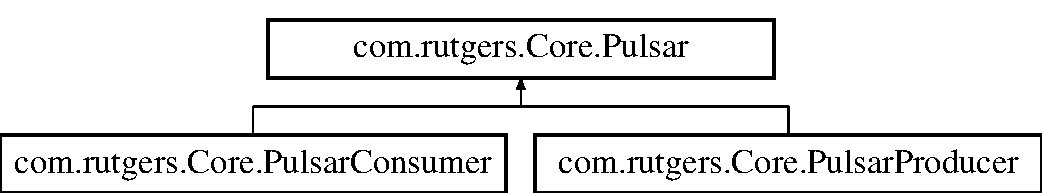
\includegraphics[height=2.000000cm]{classcom_1_1rutgers_1_1Core_1_1Pulsar}
\end{center}
\end{figure}
\subsection*{Public Member Functions}
\begin{DoxyCompactItemize}
\item 
\hyperlink{classcom_1_1rutgers_1_1Core_1_1Pulsar_a520ae30ea4c17bc8456287680348026e}{Pulsar} (Properties args)  throws I\+O\+Exception, Unknown\+Host\+Exception, Interrupted\+Exception, No\+Such\+Algorithm\+Exception 
\item 
\hyperlink{classcom_1_1rutgers_1_1Core_1_1Pulsar}{Pulsar} \hyperlink{classcom_1_1rutgers_1_1Core_1_1Pulsar_a9f6823c241f896bc76726e3d3faa43a7}{init} ()  throws I\+O\+Exception, No\+Such\+Algorithm\+Exception, Invalid\+Key\+Spec\+Exception, Unknown\+Host\+Exception, Class\+Not\+Found\+Exception 
\item 
void \hyperlink{classcom_1_1rutgers_1_1Core_1_1Pulsar_a951e085f4728c49aff0b41c5821edf6d}{replay\+Listener} (\hyperlink{interfacecom_1_1rutgers_1_1Core_1_1Listener}{Listener} o)
\item 
String \hyperlink{classcom_1_1rutgers_1_1Core_1_1Pulsar_a93cdb03ff77f49499e38aeccdb47902d}{get\+Peer\+ID} ()
\item 
void \hyperlink{classcom_1_1rutgers_1_1Core_1_1Pulsar_a76949c362c6b9fa28f1475cc3ae04123}{shutdown} ()
\item 
Peer \hyperlink{classcom_1_1rutgers_1_1Core_1_1Pulsar_af658475144e81b39e554b8ed21a19bdb}{get\+Peer} ()
\end{DoxyCompactItemize}


\subsection{Detailed Description}
This is the main A\+PI that will be used by developers to interact with R-\/\+Pulsar.

\begin{DoxyAuthor}{Author}
Eduard Giber Renart 
\end{DoxyAuthor}
\begin{DoxyVersion}{Version}
1.\+0 
\end{DoxyVersion}


\subsection{Constructor \& Destructor Documentation}
\mbox{\Hypertarget{classcom_1_1rutgers_1_1Core_1_1Pulsar_a520ae30ea4c17bc8456287680348026e}\label{classcom_1_1rutgers_1_1Core_1_1Pulsar_a520ae30ea4c17bc8456287680348026e}} 
\index{com\+::rutgers\+::\+Core\+::\+Pulsar@{com\+::rutgers\+::\+Core\+::\+Pulsar}!Pulsar@{Pulsar}}
\index{Pulsar@{Pulsar}!com\+::rutgers\+::\+Core\+::\+Pulsar@{com\+::rutgers\+::\+Core\+::\+Pulsar}}
\subsubsection{\texorpdfstring{Pulsar()}{Pulsar()}}
{\footnotesize\ttfamily com.\+rutgers.\+Core.\+Pulsar.\+Pulsar (\begin{DoxyParamCaption}\item[{Properties}]{args }\end{DoxyParamCaption}) throws I\+O\+Exception, Unknown\+Host\+Exception, Interrupted\+Exception, No\+Such\+Algorithm\+Exception}

Instantiate R-\/\+Pulsar by passing all the commands that the C\+LI class requires. 
\begin{DoxyParams}{Parameters}
{\em args} & \\
\hline
\end{DoxyParams}

\begin{DoxyExceptions}{Exceptions}
{\em I\+O\+Exception} & \\
\hline
{\em Unknown\+Host\+Exception} & \\
\hline
{\em Interrupted\+Exception} & \\
\hline
{\em No\+Such\+Algorithm\+Exception} & \\
\hline
\end{DoxyExceptions}


\subsection{Member Function Documentation}
\mbox{\Hypertarget{classcom_1_1rutgers_1_1Core_1_1Pulsar_af658475144e81b39e554b8ed21a19bdb}\label{classcom_1_1rutgers_1_1Core_1_1Pulsar_af658475144e81b39e554b8ed21a19bdb}} 
\index{com\+::rutgers\+::\+Core\+::\+Pulsar@{com\+::rutgers\+::\+Core\+::\+Pulsar}!get\+Peer@{get\+Peer}}
\index{get\+Peer@{get\+Peer}!com\+::rutgers\+::\+Core\+::\+Pulsar@{com\+::rutgers\+::\+Core\+::\+Pulsar}}
\subsubsection{\texorpdfstring{get\+Peer()}{getPeer()}}
{\footnotesize\ttfamily Peer com.\+rutgers.\+Core.\+Pulsar.\+get\+Peer (\begin{DoxyParamCaption}{ }\end{DoxyParamCaption})}

Get the Peer object. \begin{DoxyReturn}{Returns}

\end{DoxyReturn}
\mbox{\Hypertarget{classcom_1_1rutgers_1_1Core_1_1Pulsar_a93cdb03ff77f49499e38aeccdb47902d}\label{classcom_1_1rutgers_1_1Core_1_1Pulsar_a93cdb03ff77f49499e38aeccdb47902d}} 
\index{com\+::rutgers\+::\+Core\+::\+Pulsar@{com\+::rutgers\+::\+Core\+::\+Pulsar}!get\+Peer\+ID@{get\+Peer\+ID}}
\index{get\+Peer\+ID@{get\+Peer\+ID}!com\+::rutgers\+::\+Core\+::\+Pulsar@{com\+::rutgers\+::\+Core\+::\+Pulsar}}
\subsubsection{\texorpdfstring{get\+Peer\+I\+D()}{getPeerID()}}
{\footnotesize\ttfamily String com.\+rutgers.\+Core.\+Pulsar.\+get\+Peer\+ID (\begin{DoxyParamCaption}{ }\end{DoxyParamCaption})}

Get the Peer ID of this instance of the R-\/\+Pulsar. \begin{DoxyReturn}{Returns}
String with the Peer ID. 
\end{DoxyReturn}
\mbox{\Hypertarget{classcom_1_1rutgers_1_1Core_1_1Pulsar_a9f6823c241f896bc76726e3d3faa43a7}\label{classcom_1_1rutgers_1_1Core_1_1Pulsar_a9f6823c241f896bc76726e3d3faa43a7}} 
\index{com\+::rutgers\+::\+Core\+::\+Pulsar@{com\+::rutgers\+::\+Core\+::\+Pulsar}!init@{init}}
\index{init@{init}!com\+::rutgers\+::\+Core\+::\+Pulsar@{com\+::rutgers\+::\+Core\+::\+Pulsar}}
\subsubsection{\texorpdfstring{init()}{init()}}
{\footnotesize\ttfamily \hyperlink{classcom_1_1rutgers_1_1Core_1_1Pulsar}{Pulsar} com.\+rutgers.\+Core.\+Pulsar.\+init (\begin{DoxyParamCaption}{ }\end{DoxyParamCaption}) throws I\+O\+Exception, No\+Such\+Algorithm\+Exception, Invalid\+Key\+Spec\+Exception, Unknown\+Host\+Exception, Class\+Not\+Found\+Exception}

This is the first A\+PI call the needs to be performed by developers in order to init all the R-\/\+Pulsar components. \begin{DoxyReturn}{Returns}
Return and R-\/\+Pulsar object that will be used to interact with the A\+PI. 
\end{DoxyReturn}

\begin{DoxyExceptions}{Exceptions}
{\em I\+O\+Exception} & \\
\hline
{\em No\+Such\+Algorithm\+Exception} & \\
\hline
{\em Invalid\+Key\+Spec\+Exception} & \\
\hline
{\em Unknown\+Host\+Exception} & \\
\hline
{\em Class\+Not\+Found\+Exception} & \\
\hline
\end{DoxyExceptions}
\mbox{\Hypertarget{classcom_1_1rutgers_1_1Core_1_1Pulsar_a951e085f4728c49aff0b41c5821edf6d}\label{classcom_1_1rutgers_1_1Core_1_1Pulsar_a951e085f4728c49aff0b41c5821edf6d}} 
\index{com\+::rutgers\+::\+Core\+::\+Pulsar@{com\+::rutgers\+::\+Core\+::\+Pulsar}!replay\+Listener@{replay\+Listener}}
\index{replay\+Listener@{replay\+Listener}!com\+::rutgers\+::\+Core\+::\+Pulsar@{com\+::rutgers\+::\+Core\+::\+Pulsar}}
\subsubsection{\texorpdfstring{replay\+Listener()}{replayListener()}}
{\footnotesize\ttfamily void com.\+rutgers.\+Core.\+Pulsar.\+replay\+Listener (\begin{DoxyParamCaption}\item[{\hyperlink{interfacecom_1_1rutgers_1_1Core_1_1Listener}{Listener}}]{o }\end{DoxyParamCaption})}

Set the listener that will be called every time a message is received by R-\/\+Pulsar. 
\begin{DoxyParams}{Parameters}
{\em o} & Needs to tbe a \hyperlink{interfacecom_1_1rutgers_1_1Core_1_1Listener}{Listener} implemntation. \\
\hline
\end{DoxyParams}
\mbox{\Hypertarget{classcom_1_1rutgers_1_1Core_1_1Pulsar_a76949c362c6b9fa28f1475cc3ae04123}\label{classcom_1_1rutgers_1_1Core_1_1Pulsar_a76949c362c6b9fa28f1475cc3ae04123}} 
\index{com\+::rutgers\+::\+Core\+::\+Pulsar@{com\+::rutgers\+::\+Core\+::\+Pulsar}!shutdown@{shutdown}}
\index{shutdown@{shutdown}!com\+::rutgers\+::\+Core\+::\+Pulsar@{com\+::rutgers\+::\+Core\+::\+Pulsar}}
\subsubsection{\texorpdfstring{shutdown()}{shutdown()}}
{\footnotesize\ttfamily void com.\+rutgers.\+Core.\+Pulsar.\+shutdown (\begin{DoxyParamCaption}{ }\end{DoxyParamCaption})}

Stop R-\/\+Pulsar 

The documentation for this class was generated from the following file\+:\begin{DoxyCompactItemize}
\item 
src/main/java/com/rutgers/\+Core/Pulsar.\+java\end{DoxyCompactItemize}

\hypertarget{classcom_1_1rutgers_1_1Core_1_1PulsarConsumer}{}\section{com.\+rutgers.\+Core.\+Pulsar\+Consumer Class Reference}
\label{classcom_1_1rutgers_1_1Core_1_1PulsarConsumer}\index{com.\+rutgers.\+Core.\+Pulsar\+Consumer@{com.\+rutgers.\+Core.\+Pulsar\+Consumer}}
Inheritance diagram for com.\+rutgers.\+Core.\+Pulsar\+Consumer\+:\begin{figure}[H]
\begin{center}
\leavevmode
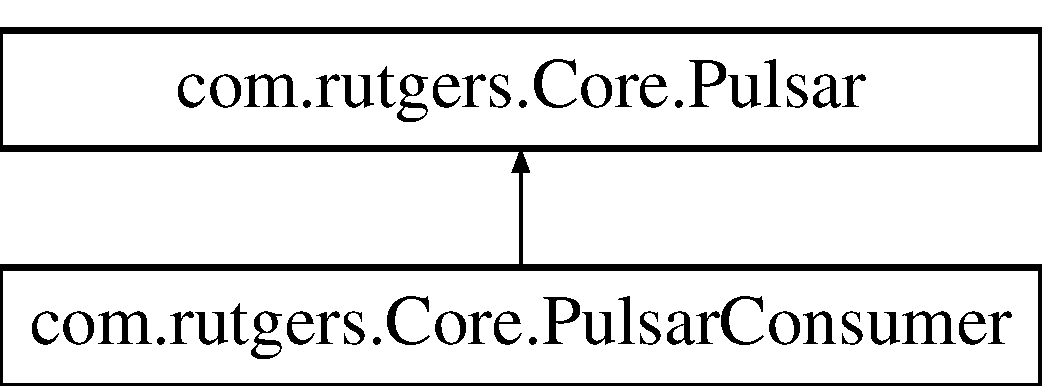
\includegraphics[height=2.000000cm]{classcom_1_1rutgers_1_1Core_1_1PulsarConsumer}
\end{center}
\end{figure}
\subsection*{Public Member Functions}
\begin{DoxyCompactItemize}
\item 
\hyperlink{classcom_1_1rutgers_1_1Core_1_1PulsarConsumer_a8363b02cc59fd0f135b0cbe46ee66715}{Pulsar\+Consumer} (Properties args)  throws I\+O\+Exception, Unknown\+Host\+Exception, Interrupted\+Exception, No\+Such\+Algorithm\+Exception 
\item 
void \hyperlink{classcom_1_1rutgers_1_1Core_1_1PulsarConsumer_ad2013ec340467446030558208403897d}{post} (Message.\+A\+R\+Message msg)  throws No\+Such\+Algorithm\+Exception, Invalid\+Key\+Spec\+Exception, Interrupted\+Exception 
\item 
void \hyperlink{classcom_1_1rutgers_1_1Core_1_1PulsarConsumer_a0e623fb8e161e9f0d920fee65a848f6d}{post} (Message.\+A\+R\+Message msg, String peer\+Id)  throws No\+Such\+Algorithm\+Exception, Invalid\+Key\+Spec\+Exception, Unknown\+Host\+Exception, Interrupted\+Exception 
\item 
Message.\+A\+R\+Message \hyperlink{classcom_1_1rutgers_1_1Core_1_1PulsarConsumer_af71ea9ed92b65eda41f352ccaa659989}{poll} (Message.\+A\+R\+Message msg, String peer\+Id)  throws No\+Such\+Algorithm\+Exception, Invalid\+Key\+Spec\+Exception, Unknown\+Host\+Exception, Interrupted\+Exception 
\item 
void \hyperlink{classcom_1_1rutgers_1_1Core_1_1PulsarConsumer_a19896243be98750670fb8688f035c2f4}{add\+Rule} (Rule rule)
\item 
void \hyperlink{classcom_1_1rutgers_1_1Core_1_1PulsarConsumer_aa90fbf7fb791809026d7536c7a6406bf}{evaluate\+Rules} (Map$<$ String, String $>$ bindings)
\end{DoxyCompactItemize}


\subsection{Detailed Description}
This is also another class that developers will use to communicate with R-\/\+Pulsar. This class will be used if we want to create an R-\/\+Pulsar cosummer.

\begin{DoxyAuthor}{Author}
Eduard Giber Renart 
\end{DoxyAuthor}
\begin{DoxyVersion}{Version}
1.\+0 
\end{DoxyVersion}


\subsection{Constructor \& Destructor Documentation}
\mbox{\Hypertarget{classcom_1_1rutgers_1_1Core_1_1PulsarConsumer_a8363b02cc59fd0f135b0cbe46ee66715}\label{classcom_1_1rutgers_1_1Core_1_1PulsarConsumer_a8363b02cc59fd0f135b0cbe46ee66715}} 
\index{com\+::rutgers\+::\+Core\+::\+Pulsar\+Consumer@{com\+::rutgers\+::\+Core\+::\+Pulsar\+Consumer}!Pulsar\+Consumer@{Pulsar\+Consumer}}
\index{Pulsar\+Consumer@{Pulsar\+Consumer}!com\+::rutgers\+::\+Core\+::\+Pulsar\+Consumer@{com\+::rutgers\+::\+Core\+::\+Pulsar\+Consumer}}
\subsubsection{\texorpdfstring{Pulsar\+Consumer()}{PulsarConsumer()}}
{\footnotesize\ttfamily com.\+rutgers.\+Core.\+Pulsar\+Consumer.\+Pulsar\+Consumer (\begin{DoxyParamCaption}\item[{Properties}]{args }\end{DoxyParamCaption}) throws I\+O\+Exception, Unknown\+Host\+Exception, Interrupted\+Exception, No\+Such\+Algorithm\+Exception}

Init the R-\/\+Pulsar instance as an R-\/\+Pulsar Consumer. 
\begin{DoxyParams}{Parameters}
{\em args} & \\
\hline
\end{DoxyParams}

\begin{DoxyExceptions}{Exceptions}
{\em I\+O\+Exception} & \\
\hline
{\em Unknown\+Host\+Exception} & \\
\hline
{\em Interrupted\+Exception} & \\
\hline
{\em No\+Such\+Algorithm\+Exception} & \\
\hline
\end{DoxyExceptions}


\subsection{Member Function Documentation}
\mbox{\Hypertarget{classcom_1_1rutgers_1_1Core_1_1PulsarConsumer_a19896243be98750670fb8688f035c2f4}\label{classcom_1_1rutgers_1_1Core_1_1PulsarConsumer_a19896243be98750670fb8688f035c2f4}} 
\index{com\+::rutgers\+::\+Core\+::\+Pulsar\+Consumer@{com\+::rutgers\+::\+Core\+::\+Pulsar\+Consumer}!add\+Rule@{add\+Rule}}
\index{add\+Rule@{add\+Rule}!com\+::rutgers\+::\+Core\+::\+Pulsar\+Consumer@{com\+::rutgers\+::\+Core\+::\+Pulsar\+Consumer}}
\subsubsection{\texorpdfstring{add\+Rule()}{addRule()}}
{\footnotesize\ttfamily void com.\+rutgers.\+Core.\+Pulsar\+Consumer.\+add\+Rule (\begin{DoxyParamCaption}\item[{Rule}]{rule }\end{DoxyParamCaption})}

Method used to add rules to make decisions. 
\begin{DoxyParams}{Parameters}
{\em rule} & Need to pass a Rule object. \\
\hline
\end{DoxyParams}
\mbox{\Hypertarget{classcom_1_1rutgers_1_1Core_1_1PulsarConsumer_aa90fbf7fb791809026d7536c7a6406bf}\label{classcom_1_1rutgers_1_1Core_1_1PulsarConsumer_aa90fbf7fb791809026d7536c7a6406bf}} 
\index{com\+::rutgers\+::\+Core\+::\+Pulsar\+Consumer@{com\+::rutgers\+::\+Core\+::\+Pulsar\+Consumer}!evaluate\+Rules@{evaluate\+Rules}}
\index{evaluate\+Rules@{evaluate\+Rules}!com\+::rutgers\+::\+Core\+::\+Pulsar\+Consumer@{com\+::rutgers\+::\+Core\+::\+Pulsar\+Consumer}}
\subsubsection{\texorpdfstring{evaluate\+Rules()}{evaluateRules()}}
{\footnotesize\ttfamily void com.\+rutgers.\+Core.\+Pulsar\+Consumer.\+evaluate\+Rules (\begin{DoxyParamCaption}\item[{Map$<$ String, String $>$}]{bindings }\end{DoxyParamCaption})}

Method used to evaluate the rules against the upcomming data. 
\begin{DoxyParams}{Parameters}
{\em bindings} & \\
\hline
\end{DoxyParams}
\mbox{\Hypertarget{classcom_1_1rutgers_1_1Core_1_1PulsarConsumer_af71ea9ed92b65eda41f352ccaa659989}\label{classcom_1_1rutgers_1_1Core_1_1PulsarConsumer_af71ea9ed92b65eda41f352ccaa659989}} 
\index{com\+::rutgers\+::\+Core\+::\+Pulsar\+Consumer@{com\+::rutgers\+::\+Core\+::\+Pulsar\+Consumer}!poll@{poll}}
\index{poll@{poll}!com\+::rutgers\+::\+Core\+::\+Pulsar\+Consumer@{com\+::rutgers\+::\+Core\+::\+Pulsar\+Consumer}}
\subsubsection{\texorpdfstring{poll()}{poll()}}
{\footnotesize\ttfamily Message.\+A\+R\+Message com.\+rutgers.\+Core.\+Pulsar\+Consumer.\+poll (\begin{DoxyParamCaption}\item[{Message.\+A\+R\+Message}]{msg,  }\item[{String}]{peer\+Id }\end{DoxyParamCaption}) throws No\+Such\+Algorithm\+Exception, Invalid\+Key\+Spec\+Exception, Unknown\+Host\+Exception, Interrupted\+Exception}

Method used to get messages from a specific peer. 
\begin{DoxyParams}{Parameters}
{\em msg} & This will contain the response message. \\
\hline
{\em peer\+Id} & This is the peer that will be sending the message. \\
\hline
\end{DoxyParams}
\begin{DoxyReturn}{Returns}

\end{DoxyReturn}

\begin{DoxyExceptions}{Exceptions}
{\em No\+Such\+Algorithm\+Exception} & \\
\hline
{\em Invalid\+Key\+Spec\+Exception} & \\
\hline
{\em Unknown\+Host\+Exception} & \\
\hline
{\em Interrupted\+Exception} & \\
\hline
\end{DoxyExceptions}
\mbox{\Hypertarget{classcom_1_1rutgers_1_1Core_1_1PulsarConsumer_ad2013ec340467446030558208403897d}\label{classcom_1_1rutgers_1_1Core_1_1PulsarConsumer_ad2013ec340467446030558208403897d}} 
\index{com\+::rutgers\+::\+Core\+::\+Pulsar\+Consumer@{com\+::rutgers\+::\+Core\+::\+Pulsar\+Consumer}!post@{post}}
\index{post@{post}!com\+::rutgers\+::\+Core\+::\+Pulsar\+Consumer@{com\+::rutgers\+::\+Core\+::\+Pulsar\+Consumer}}
\subsubsection{\texorpdfstring{post()}{post()}\hspace{0.1cm}{\footnotesize\ttfamily [1/2]}}
{\footnotesize\ttfamily void com.\+rutgers.\+Core.\+Pulsar\+Consumer.\+post (\begin{DoxyParamCaption}\item[{Message.\+A\+R\+Message}]{msg }\end{DoxyParamCaption}) throws No\+Such\+Algorithm\+Exception, Invalid\+Key\+Spec\+Exception, Interrupted\+Exception}

Method used to send a message without knowing where the reciver is located at. The space filling curve is used to route the message. 
\begin{DoxyParams}{Parameters}
{\em msg} & The AR message that we want to send. \\
\hline
\end{DoxyParams}

\begin{DoxyExceptions}{Exceptions}
{\em No\+Such\+Algorithm\+Exception} & \\
\hline
{\em Invalid\+Key\+Spec\+Exception} & \\
\hline
{\em Interrupted\+Exception} & \\
\hline
\end{DoxyExceptions}
\mbox{\Hypertarget{classcom_1_1rutgers_1_1Core_1_1PulsarConsumer_a0e623fb8e161e9f0d920fee65a848f6d}\label{classcom_1_1rutgers_1_1Core_1_1PulsarConsumer_a0e623fb8e161e9f0d920fee65a848f6d}} 
\index{com\+::rutgers\+::\+Core\+::\+Pulsar\+Consumer@{com\+::rutgers\+::\+Core\+::\+Pulsar\+Consumer}!post@{post}}
\index{post@{post}!com\+::rutgers\+::\+Core\+::\+Pulsar\+Consumer@{com\+::rutgers\+::\+Core\+::\+Pulsar\+Consumer}}
\subsubsection{\texorpdfstring{post()}{post()}\hspace{0.1cm}{\footnotesize\ttfamily [2/2]}}
{\footnotesize\ttfamily void com.\+rutgers.\+Core.\+Pulsar\+Consumer.\+post (\begin{DoxyParamCaption}\item[{Message.\+A\+R\+Message}]{msg,  }\item[{String}]{peer\+Id }\end{DoxyParamCaption}) throws No\+Such\+Algorithm\+Exception, Invalid\+Key\+Spec\+Exception, Unknown\+Host\+Exception, Interrupted\+Exception}

Send an AR message to a specific peer. In this case the space filling curve is not used. 
\begin{DoxyParams}{Parameters}
{\em msg} & The message that we want to deliver. \\
\hline
{\em peer\+Id} & The Peer Id of the recipient of the message. \\
\hline
\end{DoxyParams}

\begin{DoxyExceptions}{Exceptions}
{\em No\+Such\+Algorithm\+Exception} & \\
\hline
{\em Invalid\+Key\+Spec\+Exception} & \\
\hline
{\em Unknown\+Host\+Exception} & \\
\hline
{\em Interrupted\+Exception} & \\
\hline
\end{DoxyExceptions}


The documentation for this class was generated from the following file\+:\begin{DoxyCompactItemize}
\item 
src/main/java/com/rutgers/\+Core/Pulsar\+Consumer.\+java\end{DoxyCompactItemize}

\hypertarget{classcom_1_1rutgers_1_1Core_1_1PulsarProducer}{}\section{com.\+rutgers.\+Core.\+Pulsar\+Producer Class Reference}
\label{classcom_1_1rutgers_1_1Core_1_1PulsarProducer}\index{com.\+rutgers.\+Core.\+Pulsar\+Producer@{com.\+rutgers.\+Core.\+Pulsar\+Producer}}
Inheritance diagram for com.\+rutgers.\+Core.\+Pulsar\+Producer\+:\begin{figure}[H]
\begin{center}
\leavevmode
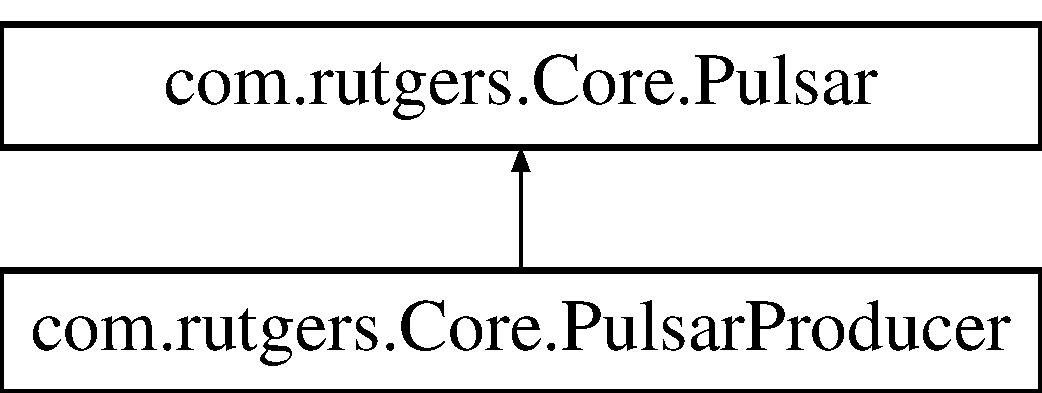
\includegraphics[height=2.000000cm]{classcom_1_1rutgers_1_1Core_1_1PulsarProducer}
\end{center}
\end{figure}
\subsection*{Public Member Functions}
\begin{DoxyCompactItemize}
\item 
\hyperlink{classcom_1_1rutgers_1_1Core_1_1PulsarProducer_a0e4b3d1d8cc83b2f0e41dbaf54a5ccfd}{Pulsar\+Producer} (Properties args)  throws I\+O\+Exception, Unknown\+Host\+Exception, Interrupted\+Exception, No\+Such\+Algorithm\+Exception 
\item 
void \hyperlink{classcom_1_1rutgers_1_1Core_1_1PulsarProducer_a70606e1822ba0cc38aa73516cc85a88a}{post} (Message.\+A\+R\+Message msg, Message.\+A\+R\+Message.\+Header.\+Profile profile)  throws No\+Such\+Algorithm\+Exception, Invalid\+Key\+Spec\+Exception, Interrupted\+Exception 
\item 
void \hyperlink{classcom_1_1rutgers_1_1Core_1_1PulsarProducer_af1cc9b050071a1089fc41fd86f83e694}{stream} (Message.\+A\+R\+Message msg, String peer\+Id)  throws No\+Such\+Algorithm\+Exception, Invalid\+Key\+Spec\+Exception, Unknown\+Host\+Exception, Interrupted\+Exception 
\item 
Peer\+Address \hyperlink{classcom_1_1rutgers_1_1Core_1_1PulsarProducer_afeedb6a5b0d46a74d533c304dd07f4b8}{create} (String peer\+Id)
\item 
void \hyperlink{classcom_1_1rutgers_1_1Core_1_1PulsarProducer_ab05285fbc423061ac0de503fbb65b362}{add\+Rule} (Rule rule)
\item 
void \hyperlink{classcom_1_1rutgers_1_1Core_1_1PulsarProducer_a8b2667977e48345fcf4025aa1b6e0123}{evaluate\+Rules} (Map$<$ String, String $>$ bindings)
\end{DoxyCompactItemize}


\subsection{Detailed Description}
This class is very similar to the \hyperlink{classcom_1_1rutgers_1_1Core_1_1PulsarConsumer}{Pulsar\+Consumer} but this time we are making a Producer. This class will be used if we want to create an R-\/\+Pulsar producer.

\begin{DoxyAuthor}{Author}
Eduard Giber Renart 
\end{DoxyAuthor}
\begin{DoxyVersion}{Version}
1.\+0 
\end{DoxyVersion}


\subsection{Constructor \& Destructor Documentation}
\mbox{\Hypertarget{classcom_1_1rutgers_1_1Core_1_1PulsarProducer_a0e4b3d1d8cc83b2f0e41dbaf54a5ccfd}\label{classcom_1_1rutgers_1_1Core_1_1PulsarProducer_a0e4b3d1d8cc83b2f0e41dbaf54a5ccfd}} 
\index{com\+::rutgers\+::\+Core\+::\+Pulsar\+Producer@{com\+::rutgers\+::\+Core\+::\+Pulsar\+Producer}!Pulsar\+Producer@{Pulsar\+Producer}}
\index{Pulsar\+Producer@{Pulsar\+Producer}!com\+::rutgers\+::\+Core\+::\+Pulsar\+Producer@{com\+::rutgers\+::\+Core\+::\+Pulsar\+Producer}}
\subsubsection{\texorpdfstring{Pulsar\+Producer()}{PulsarProducer()}}
{\footnotesize\ttfamily com.\+rutgers.\+Core.\+Pulsar\+Producer.\+Pulsar\+Producer (\begin{DoxyParamCaption}\item[{Properties}]{args }\end{DoxyParamCaption}) throws I\+O\+Exception, Unknown\+Host\+Exception, Interrupted\+Exception, No\+Such\+Algorithm\+Exception}

Init method that needs to be called in order to create an R-\/\+Pulsar producer. 
\begin{DoxyParams}{Parameters}
{\em args} & \\
\hline
\end{DoxyParams}

\begin{DoxyExceptions}{Exceptions}
{\em I\+O\+Exception} & \\
\hline
{\em Unknown\+Host\+Exception} & \\
\hline
{\em Interrupted\+Exception} & \\
\hline
{\em No\+Such\+Algorithm\+Exception} & \\
\hline
\end{DoxyExceptions}


\subsection{Member Function Documentation}
\mbox{\Hypertarget{classcom_1_1rutgers_1_1Core_1_1PulsarProducer_ab05285fbc423061ac0de503fbb65b362}\label{classcom_1_1rutgers_1_1Core_1_1PulsarProducer_ab05285fbc423061ac0de503fbb65b362}} 
\index{com\+::rutgers\+::\+Core\+::\+Pulsar\+Producer@{com\+::rutgers\+::\+Core\+::\+Pulsar\+Producer}!add\+Rule@{add\+Rule}}
\index{add\+Rule@{add\+Rule}!com\+::rutgers\+::\+Core\+::\+Pulsar\+Producer@{com\+::rutgers\+::\+Core\+::\+Pulsar\+Producer}}
\subsubsection{\texorpdfstring{add\+Rule()}{addRule()}}
{\footnotesize\ttfamily void com.\+rutgers.\+Core.\+Pulsar\+Producer.\+add\+Rule (\begin{DoxyParamCaption}\item[{Rule}]{rule }\end{DoxyParamCaption})}

Add a rule in to the rule engine. 
\begin{DoxyParams}{Parameters}
{\em rule} & \\
\hline
\end{DoxyParams}
\mbox{\Hypertarget{classcom_1_1rutgers_1_1Core_1_1PulsarProducer_afeedb6a5b0d46a74d533c304dd07f4b8}\label{classcom_1_1rutgers_1_1Core_1_1PulsarProducer_afeedb6a5b0d46a74d533c304dd07f4b8}} 
\index{com\+::rutgers\+::\+Core\+::\+Pulsar\+Producer@{com\+::rutgers\+::\+Core\+::\+Pulsar\+Producer}!create@{create}}
\index{create@{create}!com\+::rutgers\+::\+Core\+::\+Pulsar\+Producer@{com\+::rutgers\+::\+Core\+::\+Pulsar\+Producer}}
\subsubsection{\texorpdfstring{create()}{create()}}
{\footnotesize\ttfamily Peer\+Address com.\+rutgers.\+Core.\+Pulsar\+Producer.\+create (\begin{DoxyParamCaption}\item[{String}]{peer\+Id }\end{DoxyParamCaption})}

Method used to change teh peer Id of and \hyperlink{classcom_1_1rutgers_1_1Core_1_1RP}{RP}. 
\begin{DoxyParams}{Parameters}
{\em peer\+Id} & \\
\hline
\end{DoxyParams}
\begin{DoxyReturn}{Returns}

\end{DoxyReturn}
\mbox{\Hypertarget{classcom_1_1rutgers_1_1Core_1_1PulsarProducer_a8b2667977e48345fcf4025aa1b6e0123}\label{classcom_1_1rutgers_1_1Core_1_1PulsarProducer_a8b2667977e48345fcf4025aa1b6e0123}} 
\index{com\+::rutgers\+::\+Core\+::\+Pulsar\+Producer@{com\+::rutgers\+::\+Core\+::\+Pulsar\+Producer}!evaluate\+Rules@{evaluate\+Rules}}
\index{evaluate\+Rules@{evaluate\+Rules}!com\+::rutgers\+::\+Core\+::\+Pulsar\+Producer@{com\+::rutgers\+::\+Core\+::\+Pulsar\+Producer}}
\subsubsection{\texorpdfstring{evaluate\+Rules()}{evaluateRules()}}
{\footnotesize\ttfamily void com.\+rutgers.\+Core.\+Pulsar\+Producer.\+evaluate\+Rules (\begin{DoxyParamCaption}\item[{Map$<$ String, String $>$}]{bindings }\end{DoxyParamCaption})}

Evaluate the rules 
\begin{DoxyParams}{Parameters}
{\em bindings} & \\
\hline
\end{DoxyParams}
\mbox{\Hypertarget{classcom_1_1rutgers_1_1Core_1_1PulsarProducer_a70606e1822ba0cc38aa73516cc85a88a}\label{classcom_1_1rutgers_1_1Core_1_1PulsarProducer_a70606e1822ba0cc38aa73516cc85a88a}} 
\index{com\+::rutgers\+::\+Core\+::\+Pulsar\+Producer@{com\+::rutgers\+::\+Core\+::\+Pulsar\+Producer}!post@{post}}
\index{post@{post}!com\+::rutgers\+::\+Core\+::\+Pulsar\+Producer@{com\+::rutgers\+::\+Core\+::\+Pulsar\+Producer}}
\subsubsection{\texorpdfstring{post()}{post()}}
{\footnotesize\ttfamily void com.\+rutgers.\+Core.\+Pulsar\+Producer.\+post (\begin{DoxyParamCaption}\item[{Message.\+A\+R\+Message}]{msg,  }\item[{Message.\+A\+R\+Message.\+Header.\+Profile}]{profile }\end{DoxyParamCaption}) throws No\+Such\+Algorithm\+Exception, Invalid\+Key\+Spec\+Exception, Interrupted\+Exception}

This method is used to send a message using the profile. The space filling curve will be used to route the message. 
\begin{DoxyParams}{Parameters}
{\em msg} & \hyperlink{classcom_1_1rutgers_1_1Core_1_1Message}{Message} to send. \\
\hline
{\em profile} & This will determine who will receive the message. \\
\hline
\end{DoxyParams}

\begin{DoxyExceptions}{Exceptions}
{\em No\+Such\+Algorithm\+Exception} & \\
\hline
{\em Invalid\+Key\+Spec\+Exception} & \\
\hline
{\em Interrupted\+Exception} & \\
\hline
\end{DoxyExceptions}
\mbox{\Hypertarget{classcom_1_1rutgers_1_1Core_1_1PulsarProducer_af1cc9b050071a1089fc41fd86f83e694}\label{classcom_1_1rutgers_1_1Core_1_1PulsarProducer_af1cc9b050071a1089fc41fd86f83e694}} 
\index{com\+::rutgers\+::\+Core\+::\+Pulsar\+Producer@{com\+::rutgers\+::\+Core\+::\+Pulsar\+Producer}!stream@{stream}}
\index{stream@{stream}!com\+::rutgers\+::\+Core\+::\+Pulsar\+Producer@{com\+::rutgers\+::\+Core\+::\+Pulsar\+Producer}}
\subsubsection{\texorpdfstring{stream()}{stream()}}
{\footnotesize\ttfamily void com.\+rutgers.\+Core.\+Pulsar\+Producer.\+stream (\begin{DoxyParamCaption}\item[{Message.\+A\+R\+Message}]{msg,  }\item[{String}]{peer\+Id }\end{DoxyParamCaption}) throws No\+Such\+Algorithm\+Exception, Invalid\+Key\+Spec\+Exception, Unknown\+Host\+Exception, Interrupted\+Exception}

Stream multiple messages to an specific peer. 
\begin{DoxyParams}{Parameters}
{\em msg} & \hyperlink{classcom_1_1rutgers_1_1Core_1_1Message}{Message} to send. \\
\hline
{\em peer\+Id} & Peer Id of the peer that will receive the message. \\
\hline
\end{DoxyParams}

\begin{DoxyExceptions}{Exceptions}
{\em No\+Such\+Algorithm\+Exception} & \\
\hline
{\em Invalid\+Key\+Spec\+Exception} & \\
\hline
{\em Unknown\+Host\+Exception} & \\
\hline
{\em Interrupted\+Exception} & \\
\hline
\end{DoxyExceptions}


The documentation for this class was generated from the following file\+:\begin{DoxyCompactItemize}
\item 
src/main/java/com/rutgers/\+Core/Pulsar\+Producer.\+java\end{DoxyCompactItemize}

\hypertarget{classcom_1_1rutgers_1_1Core_1_1QueueManager}{}\section{com.\+rutgers.\+Core.\+Queue\+Manager Class Reference}
\label{classcom_1_1rutgers_1_1Core_1_1QueueManager}\index{com.\+rutgers.\+Core.\+Queue\+Manager@{com.\+rutgers.\+Core.\+Queue\+Manager}}


\subsection{Detailed Description}
\begin{DoxyAuthor}{Author}
eduard 
\end{DoxyAuthor}


The documentation for this class was generated from the following file\+:\begin{DoxyCompactItemize}
\item 
src/main/java/com/rutgers/\+Core/Queue\+Manager.\+java\end{DoxyCompactItemize}

\hypertarget{classcom_1_1rutgers_1_1Tree_1_1RedBlackTree}{}\section{com.\+rutgers.\+Tree.\+Red\+Black\+Tree Class Reference}
\label{classcom_1_1rutgers_1_1Tree_1_1RedBlackTree}\index{com.\+rutgers.\+Tree.\+Red\+Black\+Tree@{com.\+rutgers.\+Tree.\+Red\+Black\+Tree}}
Inheritance diagram for com.\+rutgers.\+Tree.\+Red\+Black\+Tree\+:\begin{figure}[H]
\begin{center}
\leavevmode
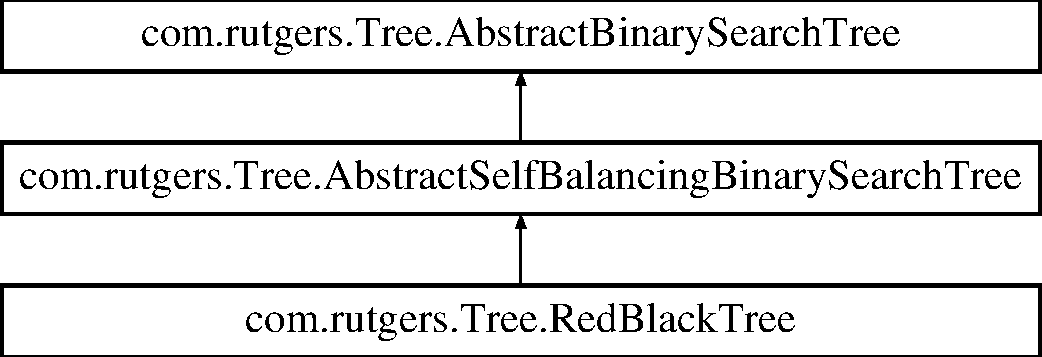
\includegraphics[height=3.000000cm]{classcom_1_1rutgers_1_1Tree_1_1RedBlackTree}
\end{center}
\end{figure}
\subsection*{Public Member Functions}
\begin{DoxyCompactItemize}
\item 
Node \hyperlink{classcom_1_1rutgers_1_1Tree_1_1RedBlackTree_a7677220dd9ac20292cbabb0c80d4ce3d}{insert} (int element)
\end{DoxyCompactItemize}
\subsection*{Protected Member Functions}
\begin{DoxyCompactItemize}
\item 
Node \hyperlink{classcom_1_1rutgers_1_1Tree_1_1RedBlackTree_a32edb63c284dad19e7feb2c8ae61366d}{delete} (Node delete\+Node)
\item 
Node \hyperlink{classcom_1_1rutgers_1_1Tree_1_1RedBlackTree_a44da4e60e7dafdf6e5d290be07ee4c8a}{create\+Node} (int value, Node parent, Node left, Node right)
\item 
Node \hyperlink{classcom_1_1rutgers_1_1Tree_1_1RedBlackTree_aa568e5fd51bd7b1b08fb52f5eaf4ba25}{get\+Minimum} (Node node)
\item 
Node \hyperlink{classcom_1_1rutgers_1_1Tree_1_1RedBlackTree_a2fc7ea91e9e22df233f8abe9acada0c1}{get\+Maximum} (Node node)
\item 
Node \hyperlink{classcom_1_1rutgers_1_1Tree_1_1RedBlackTree_a5265e4d750913f992eec7cec4b1082bf}{rotate\+Left} (Node node)
\item 
Node \hyperlink{classcom_1_1rutgers_1_1Tree_1_1RedBlackTree_a78a3a6b0847ca0f071dabf45bef4f924}{rotate\+Right} (Node node)
\end{DoxyCompactItemize}
\subsection*{Additional Inherited Members}


\subsection{Detailed Description}
\begin{DoxyAuthor}{Author}
eduard 
\end{DoxyAuthor}


\subsection{Member Function Documentation}
\mbox{\Hypertarget{classcom_1_1rutgers_1_1Tree_1_1RedBlackTree_a44da4e60e7dafdf6e5d290be07ee4c8a}\label{classcom_1_1rutgers_1_1Tree_1_1RedBlackTree_a44da4e60e7dafdf6e5d290be07ee4c8a}} 
\index{com\+::rutgers\+::\+Tree\+::\+Red\+Black\+Tree@{com\+::rutgers\+::\+Tree\+::\+Red\+Black\+Tree}!create\+Node@{create\+Node}}
\index{create\+Node@{create\+Node}!com\+::rutgers\+::\+Tree\+::\+Red\+Black\+Tree@{com\+::rutgers\+::\+Tree\+::\+Red\+Black\+Tree}}
\subsubsection{\texorpdfstring{create\+Node()}{createNode()}}
{\footnotesize\ttfamily Node com.\+rutgers.\+Tree.\+Red\+Black\+Tree.\+create\+Node (\begin{DoxyParamCaption}\item[{int}]{value,  }\item[{Node}]{parent,  }\item[{Node}]{left,  }\item[{Node}]{right }\end{DoxyParamCaption})\hspace{0.3cm}{\ttfamily [protected]}}

\begin{DoxySeeAlso}{See also}
org.\+intelligentjava.\+algos.\+trees.\+Abstract\+Binary\+Search\+Tree\+::create\+Node(int, org.\+intelligentjava.\+algos.\+trees.\+Abstract\+Binary\+Search\+Tree.\+Node, org.\+intelligentjava.\+algos.\+trees.\+Abstract\+Binary\+Search\+Tree.\+Node, org.\+intelligentjava.\+algos.\+trees.\+Abstract\+Binary\+Search\+Tree.\+Node) 
\end{DoxySeeAlso}
\mbox{\Hypertarget{classcom_1_1rutgers_1_1Tree_1_1RedBlackTree_a32edb63c284dad19e7feb2c8ae61366d}\label{classcom_1_1rutgers_1_1Tree_1_1RedBlackTree_a32edb63c284dad19e7feb2c8ae61366d}} 
\index{com\+::rutgers\+::\+Tree\+::\+Red\+Black\+Tree@{com\+::rutgers\+::\+Tree\+::\+Red\+Black\+Tree}!delete@{delete}}
\index{delete@{delete}!com\+::rutgers\+::\+Tree\+::\+Red\+Black\+Tree@{com\+::rutgers\+::\+Tree\+::\+Red\+Black\+Tree}}
\subsubsection{\texorpdfstring{delete()}{delete()}}
{\footnotesize\ttfamily Node com.\+rutgers.\+Tree.\+Red\+Black\+Tree.\+delete (\begin{DoxyParamCaption}\item[{Node}]{delete\+Node }\end{DoxyParamCaption})\hspace{0.3cm}{\ttfamily [protected]}}

Slightly modified delete routine for red-\/black tree.\mbox{\Hypertarget{classcom_1_1rutgers_1_1Tree_1_1RedBlackTree_a2fc7ea91e9e22df233f8abe9acada0c1}\label{classcom_1_1rutgers_1_1Tree_1_1RedBlackTree_a2fc7ea91e9e22df233f8abe9acada0c1}} 
\index{com\+::rutgers\+::\+Tree\+::\+Red\+Black\+Tree@{com\+::rutgers\+::\+Tree\+::\+Red\+Black\+Tree}!get\+Maximum@{get\+Maximum}}
\index{get\+Maximum@{get\+Maximum}!com\+::rutgers\+::\+Tree\+::\+Red\+Black\+Tree@{com\+::rutgers\+::\+Tree\+::\+Red\+Black\+Tree}}
\subsubsection{\texorpdfstring{get\+Maximum()}{getMaximum()}}
{\footnotesize\ttfamily Node com.\+rutgers.\+Tree.\+Red\+Black\+Tree.\+get\+Maximum (\begin{DoxyParamCaption}\item[{Node}]{node }\end{DoxyParamCaption})\hspace{0.3cm}{\ttfamily [protected]}}

\mbox{\Hypertarget{classcom_1_1rutgers_1_1Tree_1_1RedBlackTree_aa568e5fd51bd7b1b08fb52f5eaf4ba25}\label{classcom_1_1rutgers_1_1Tree_1_1RedBlackTree_aa568e5fd51bd7b1b08fb52f5eaf4ba25}} 
\index{com\+::rutgers\+::\+Tree\+::\+Red\+Black\+Tree@{com\+::rutgers\+::\+Tree\+::\+Red\+Black\+Tree}!get\+Minimum@{get\+Minimum}}
\index{get\+Minimum@{get\+Minimum}!com\+::rutgers\+::\+Tree\+::\+Red\+Black\+Tree@{com\+::rutgers\+::\+Tree\+::\+Red\+Black\+Tree}}
\subsubsection{\texorpdfstring{get\+Minimum()}{getMinimum()}}
{\footnotesize\ttfamily Node com.\+rutgers.\+Tree.\+Red\+Black\+Tree.\+get\+Minimum (\begin{DoxyParamCaption}\item[{Node}]{node }\end{DoxyParamCaption})\hspace{0.3cm}{\ttfamily [protected]}}

\mbox{\Hypertarget{classcom_1_1rutgers_1_1Tree_1_1RedBlackTree_a7677220dd9ac20292cbabb0c80d4ce3d}\label{classcom_1_1rutgers_1_1Tree_1_1RedBlackTree_a7677220dd9ac20292cbabb0c80d4ce3d}} 
\index{com\+::rutgers\+::\+Tree\+::\+Red\+Black\+Tree@{com\+::rutgers\+::\+Tree\+::\+Red\+Black\+Tree}!insert@{insert}}
\index{insert@{insert}!com\+::rutgers\+::\+Tree\+::\+Red\+Black\+Tree@{com\+::rutgers\+::\+Tree\+::\+Red\+Black\+Tree}}
\subsubsection{\texorpdfstring{insert()}{insert()}}
{\footnotesize\ttfamily Node com.\+rutgers.\+Tree.\+Red\+Black\+Tree.\+insert (\begin{DoxyParamCaption}\item[{int}]{element }\end{DoxyParamCaption})}

\begin{DoxySeeAlso}{See also}
org.\+intelligentjava.\+algos.\+trees.\+Abstract\+Binary\+Search\+Tree\+::insert(int) 
\end{DoxySeeAlso}
\mbox{\Hypertarget{classcom_1_1rutgers_1_1Tree_1_1RedBlackTree_a5265e4d750913f992eec7cec4b1082bf}\label{classcom_1_1rutgers_1_1Tree_1_1RedBlackTree_a5265e4d750913f992eec7cec4b1082bf}} 
\index{com\+::rutgers\+::\+Tree\+::\+Red\+Black\+Tree@{com\+::rutgers\+::\+Tree\+::\+Red\+Black\+Tree}!rotate\+Left@{rotate\+Left}}
\index{rotate\+Left@{rotate\+Left}!com\+::rutgers\+::\+Tree\+::\+Red\+Black\+Tree@{com\+::rutgers\+::\+Tree\+::\+Red\+Black\+Tree}}
\subsubsection{\texorpdfstring{rotate\+Left()}{rotateLeft()}}
{\footnotesize\ttfamily Node com.\+rutgers.\+Tree.\+Red\+Black\+Tree.\+rotate\+Left (\begin{DoxyParamCaption}\item[{Node}]{node }\end{DoxyParamCaption})\hspace{0.3cm}{\ttfamily [protected]}}

\mbox{\Hypertarget{classcom_1_1rutgers_1_1Tree_1_1RedBlackTree_a78a3a6b0847ca0f071dabf45bef4f924}\label{classcom_1_1rutgers_1_1Tree_1_1RedBlackTree_a78a3a6b0847ca0f071dabf45bef4f924}} 
\index{com\+::rutgers\+::\+Tree\+::\+Red\+Black\+Tree@{com\+::rutgers\+::\+Tree\+::\+Red\+Black\+Tree}!rotate\+Right@{rotate\+Right}}
\index{rotate\+Right@{rotate\+Right}!com\+::rutgers\+::\+Tree\+::\+Red\+Black\+Tree@{com\+::rutgers\+::\+Tree\+::\+Red\+Black\+Tree}}
\subsubsection{\texorpdfstring{rotate\+Right()}{rotateRight()}}
{\footnotesize\ttfamily Node com.\+rutgers.\+Tree.\+Red\+Black\+Tree.\+rotate\+Right (\begin{DoxyParamCaption}\item[{Node}]{node }\end{DoxyParamCaption})\hspace{0.3cm}{\ttfamily [protected]}}



The documentation for this class was generated from the following file\+:\begin{DoxyCompactItemize}
\item 
src/main/java/com/rutgers/\+Tree/Red\+Black\+Tree.\+java\end{DoxyCompactItemize}

\hypertarget{classcom_1_1rutgers_1_1DB_1_1RocksDBMS}{}\section{com.\+rutgers.\+D\+B.\+Rocks\+D\+B\+MS Class Reference}
\label{classcom_1_1rutgers_1_1DB_1_1RocksDBMS}\index{com.\+rutgers.\+D\+B.\+Rocks\+D\+B\+MS@{com.\+rutgers.\+D\+B.\+Rocks\+D\+B\+MS}}
\subsection*{Public Member Functions}
\begin{DoxyCompactItemize}
\item 
void \hyperlink{classcom_1_1rutgers_1_1DB_1_1RocksDBMS_a3457d063685184152707f7e25b7bcb6c}{put\+Data} (String\mbox{[}$\,$\mbox{]} id, Number160\mbox{[}$\,$\mbox{]} keys)
\item 
void \hyperlink{classcom_1_1rutgers_1_1DB_1_1RocksDBMS_a8f19edec5bd60c75362223c880cd8a2f}{put\+Data} (byte\mbox{[}$\,$\mbox{]} id, Number160... keys)
\item 
void \hyperlink{classcom_1_1rutgers_1_1DB_1_1RocksDBMS_a61ac1a0207af7dff4cc4de59f10fbcc8}{put\+Interest} (byte\mbox{[}$\,$\mbox{]} id, Number160... keys)
\item 
Array\+List$<$ byte\mbox{[}$\,$\mbox{]}$>$ \hyperlink{classcom_1_1rutgers_1_1DB_1_1RocksDBMS_a58fdef51ec9602cabebb09a2448dc3c6}{get\+Interest} (Number160... keys)
\item 
void \hyperlink{classcom_1_1rutgers_1_1DB_1_1RocksDBMS_a00912a8d8d29f3692ffb6974ad7f683c}{delete\+Interest} (Number160... keys)
\item 
void \hyperlink{classcom_1_1rutgers_1_1DB_1_1RocksDBMS_a4231ce755ceddab79d715d44a9f98d7d}{close} ()
\end{DoxyCompactItemize}


\subsection{Detailed Description}
This class implements some basic functionality of \hyperlink{classcom_1_1rutgers_1_1DB_1_1RocksDBMS}{Rocks\+D\+B\+MS}. This class is used to store all the profiles in the system. This class in the paper is decribed as the matching engein.

\begin{DoxyAuthor}{Author}
Eduard Gibert Renart 
\end{DoxyAuthor}
\begin{DoxyVersion}{Version}
1.\+0 
\end{DoxyVersion}


\subsection{Member Function Documentation}
\mbox{\Hypertarget{classcom_1_1rutgers_1_1DB_1_1RocksDBMS_a4231ce755ceddab79d715d44a9f98d7d}\label{classcom_1_1rutgers_1_1DB_1_1RocksDBMS_a4231ce755ceddab79d715d44a9f98d7d}} 
\index{com\+::rutgers\+::\+D\+B\+::\+Rocks\+D\+B\+MS@{com\+::rutgers\+::\+D\+B\+::\+Rocks\+D\+B\+MS}!close@{close}}
\index{close@{close}!com\+::rutgers\+::\+D\+B\+::\+Rocks\+D\+B\+MS@{com\+::rutgers\+::\+D\+B\+::\+Rocks\+D\+B\+MS}}
\subsubsection{\texorpdfstring{close()}{close()}}
{\footnotesize\ttfamily void com.\+rutgers.\+D\+B.\+Rocks\+D\+B\+M\+S.\+close (\begin{DoxyParamCaption}{ }\end{DoxyParamCaption})}

Close the DB. \mbox{\Hypertarget{classcom_1_1rutgers_1_1DB_1_1RocksDBMS_a00912a8d8d29f3692ffb6974ad7f683c}\label{classcom_1_1rutgers_1_1DB_1_1RocksDBMS_a00912a8d8d29f3692ffb6974ad7f683c}} 
\index{com\+::rutgers\+::\+D\+B\+::\+Rocks\+D\+B\+MS@{com\+::rutgers\+::\+D\+B\+::\+Rocks\+D\+B\+MS}!delete\+Interest@{delete\+Interest}}
\index{delete\+Interest@{delete\+Interest}!com\+::rutgers\+::\+D\+B\+::\+Rocks\+D\+B\+MS@{com\+::rutgers\+::\+D\+B\+::\+Rocks\+D\+B\+MS}}
\subsubsection{\texorpdfstring{delete\+Interest()}{deleteInterest()}}
{\footnotesize\ttfamily void com.\+rutgers.\+D\+B.\+Rocks\+D\+B\+M\+S.\+delete\+Interest (\begin{DoxyParamCaption}\item[{Number160...}]{keys }\end{DoxyParamCaption})}

Delete multiple interest profiles from the DB. 
\begin{DoxyParams}{Parameters}
{\em keys} & \\
\hline
\end{DoxyParams}
\mbox{\Hypertarget{classcom_1_1rutgers_1_1DB_1_1RocksDBMS_a58fdef51ec9602cabebb09a2448dc3c6}\label{classcom_1_1rutgers_1_1DB_1_1RocksDBMS_a58fdef51ec9602cabebb09a2448dc3c6}} 
\index{com\+::rutgers\+::\+D\+B\+::\+Rocks\+D\+B\+MS@{com\+::rutgers\+::\+D\+B\+::\+Rocks\+D\+B\+MS}!get\+Interest@{get\+Interest}}
\index{get\+Interest@{get\+Interest}!com\+::rutgers\+::\+D\+B\+::\+Rocks\+D\+B\+MS@{com\+::rutgers\+::\+D\+B\+::\+Rocks\+D\+B\+MS}}
\subsubsection{\texorpdfstring{get\+Interest()}{getInterest()}}
{\footnotesize\ttfamily Array\+List$<$byte\mbox{[}$\,$\mbox{]}$>$ com.\+rutgers.\+D\+B.\+Rocks\+D\+B\+M\+S.\+get\+Interest (\begin{DoxyParamCaption}\item[{Number160...}]{keys }\end{DoxyParamCaption})}

Check if a set of interest profiles are present in the DB. 
\begin{DoxyParams}{Parameters}
{\em keys} & \\
\hline
\end{DoxyParams}
\begin{DoxyReturn}{Returns}

\end{DoxyReturn}
\mbox{\Hypertarget{classcom_1_1rutgers_1_1DB_1_1RocksDBMS_a3457d063685184152707f7e25b7bcb6c}\label{classcom_1_1rutgers_1_1DB_1_1RocksDBMS_a3457d063685184152707f7e25b7bcb6c}} 
\index{com\+::rutgers\+::\+D\+B\+::\+Rocks\+D\+B\+MS@{com\+::rutgers\+::\+D\+B\+::\+Rocks\+D\+B\+MS}!put\+Data@{put\+Data}}
\index{put\+Data@{put\+Data}!com\+::rutgers\+::\+D\+B\+::\+Rocks\+D\+B\+MS@{com\+::rutgers\+::\+D\+B\+::\+Rocks\+D\+B\+MS}}
\subsubsection{\texorpdfstring{put\+Data()}{putData()}\hspace{0.1cm}{\footnotesize\ttfamily [1/2]}}
{\footnotesize\ttfamily void com.\+rutgers.\+D\+B.\+Rocks\+D\+B\+M\+S.\+put\+Data (\begin{DoxyParamCaption}\item[{String \mbox{[}$\,$\mbox{]}}]{id,  }\item[{Number160 \mbox{[}$\,$\mbox{]}}]{keys }\end{DoxyParamCaption})}

Store a single element into the database. 
\begin{DoxyParams}{Parameters}
{\em id} & \\
\hline
{\em keys} & \\
\hline
\end{DoxyParams}
\mbox{\Hypertarget{classcom_1_1rutgers_1_1DB_1_1RocksDBMS_a8f19edec5bd60c75362223c880cd8a2f}\label{classcom_1_1rutgers_1_1DB_1_1RocksDBMS_a8f19edec5bd60c75362223c880cd8a2f}} 
\index{com\+::rutgers\+::\+D\+B\+::\+Rocks\+D\+B\+MS@{com\+::rutgers\+::\+D\+B\+::\+Rocks\+D\+B\+MS}!put\+Data@{put\+Data}}
\index{put\+Data@{put\+Data}!com\+::rutgers\+::\+D\+B\+::\+Rocks\+D\+B\+MS@{com\+::rutgers\+::\+D\+B\+::\+Rocks\+D\+B\+MS}}
\subsubsection{\texorpdfstring{put\+Data()}{putData()}\hspace{0.1cm}{\footnotesize\ttfamily [2/2]}}
{\footnotesize\ttfamily void com.\+rutgers.\+D\+B.\+Rocks\+D\+B\+M\+S.\+put\+Data (\begin{DoxyParamCaption}\item[{byte \mbox{[}$\,$\mbox{]}}]{id,  }\item[{Number160...}]{keys }\end{DoxyParamCaption})}

Store multiple elements into the database. 
\begin{DoxyParams}{Parameters}
{\em id} & \\
\hline
{\em keys} & \\
\hline
\end{DoxyParams}
\mbox{\Hypertarget{classcom_1_1rutgers_1_1DB_1_1RocksDBMS_a61ac1a0207af7dff4cc4de59f10fbcc8}\label{classcom_1_1rutgers_1_1DB_1_1RocksDBMS_a61ac1a0207af7dff4cc4de59f10fbcc8}} 
\index{com\+::rutgers\+::\+D\+B\+::\+Rocks\+D\+B\+MS@{com\+::rutgers\+::\+D\+B\+::\+Rocks\+D\+B\+MS}!put\+Interest@{put\+Interest}}
\index{put\+Interest@{put\+Interest}!com\+::rutgers\+::\+D\+B\+::\+Rocks\+D\+B\+MS@{com\+::rutgers\+::\+D\+B\+::\+Rocks\+D\+B\+MS}}
\subsubsection{\texorpdfstring{put\+Interest()}{putInterest()}}
{\footnotesize\ttfamily void com.\+rutgers.\+D\+B.\+Rocks\+D\+B\+M\+S.\+put\+Interest (\begin{DoxyParamCaption}\item[{byte \mbox{[}$\,$\mbox{]}}]{id,  }\item[{Number160...}]{keys }\end{DoxyParamCaption})}

Store multiple interest profiles into the DB. 
\begin{DoxyParams}{Parameters}
{\em id} & \\
\hline
{\em keys} & \\
\hline
\end{DoxyParams}


The documentation for this class was generated from the following file\+:\begin{DoxyCompactItemize}
\item 
src/main/java/com/rutgers/\+D\+B/Rocks\+D\+B\+M\+S.\+java\end{DoxyCompactItemize}

\hypertarget{classcom_1_1rutgers_1_1DB_1_1RocksDHT}{}\section{com.\+rutgers.\+D\+B.\+Rocks\+D\+HT Class Reference}
\label{classcom_1_1rutgers_1_1DB_1_1RocksDHT}\index{com.\+rutgers.\+D\+B.\+Rocks\+D\+HT@{com.\+rutgers.\+D\+B.\+Rocks\+D\+HT}}


Inherits Storage.



\subsection{Detailed Description}
This class implements the D\+HT functionality. It implements the Storage abstraction from Tom\+P2P.

\begin{DoxyAuthor}{Author}
eduard 
\end{DoxyAuthor}


The documentation for this class was generated from the following file\+:\begin{DoxyCompactItemize}
\item 
src/main/java/com/rutgers/\+D\+B/Rocks\+D\+H\+T.\+java\end{DoxyCompactItemize}

\hypertarget{classcom_1_1rutgers_1_1Core_1_1RP}{}\section{com.\+rutgers.\+Core.\+RP Class Reference}
\label{classcom_1_1rutgers_1_1Core_1_1RP}\index{com.\+rutgers.\+Core.\+RP@{com.\+rutgers.\+Core.\+RP}}
Inheritance diagram for com.\+rutgers.\+Core.\+RP\+:\begin{figure}[H]
\begin{center}
\leavevmode
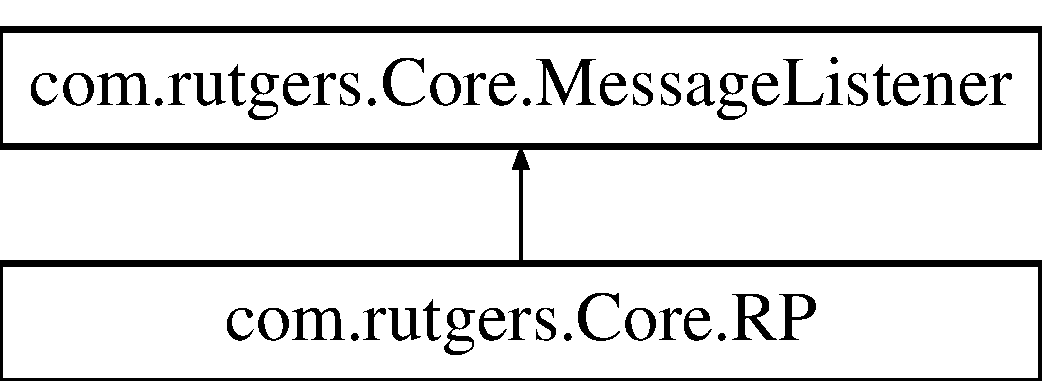
\includegraphics[height=2.000000cm]{classcom_1_1rutgers_1_1Core_1_1RP}
\end{center}
\end{figure}
\subsection*{Additional Inherited Members}


\subsection{Detailed Description}
\begin{DoxyAuthor}{Author}
eduard 
\end{DoxyAuthor}


The documentation for this class was generated from the following file\+:\begin{DoxyCompactItemize}
\item 
src/main/java/com/rutgers/\+Core/R\+P.\+java\end{DoxyCompactItemize}

\hypertarget{enumcom_1_1rutgers_1_1Core_1_1Message_1_1ARMessage_1_1RPType}{}\section{com.\+rutgers.\+Core.\+Message.\+A\+R\+Message.\+R\+P\+Type Enum Reference}
\label{enumcom_1_1rutgers_1_1Core_1_1Message_1_1ARMessage_1_1RPType}\index{com.\+rutgers.\+Core.\+Message.\+A\+R\+Message.\+R\+P\+Type@{com.\+rutgers.\+Core.\+Message.\+A\+R\+Message.\+R\+P\+Type}}


Inherits Protocol\+Message\+Enum.

\subsection*{Static Public Member Functions}
\begin{DoxyCompactItemize}
\item 
.lang.\+Deprecated static \hyperlink{enumcom_1_1rutgers_1_1Core_1_1Message_1_1ARMessage_1_1RPType}{R\+P\+Type} \hyperlink{enumcom_1_1rutgers_1_1Core_1_1Message_1_1ARMessage_1_1RPType_aa300501b5400695678c229e3d7f6eff3}{value\+Of} (int value)
\end{DoxyCompactItemize}
\subsection*{Public Attributes}
\begin{DoxyCompactItemize}
\item 
\hyperlink{enumcom_1_1rutgers_1_1Core_1_1Message_1_1ARMessage_1_1RPType_a5ad2d7bf858b18aa8bd99453e42d758c}{A\+R\+\_\+\+C\+O\+N\+S\+U\+M\+ER} =(0)
\item 
\hyperlink{enumcom_1_1rutgers_1_1Core_1_1Message_1_1ARMessage_1_1RPType_a7bc13bd5f7ee4ba265c00bb2a26cf74c}{A\+R\+\_\+\+U\+S\+ER} =(1)
\item 
\hyperlink{enumcom_1_1rutgers_1_1Core_1_1Message_1_1ARMessage_1_1RPType_adad71551f5fbf1c673d2bcfac5326877}{A\+R\+\_\+\+P\+R\+O\+D\+U\+C\+ER} =(2)
\item 
\hyperlink{enumcom_1_1rutgers_1_1Core_1_1Message_1_1ARMessage_1_1RPType_ac74adfe3c76ba0a99000b58fea4ce2b3}{A\+R\+\_\+\+A\+N\+D\+R\+O\+I\+D\+\_\+\+U\+S\+ER} =(3)
\item 
\hyperlink{enumcom_1_1rutgers_1_1Core_1_1Message_1_1ARMessage_1_1RPType_ada9191863da74aeb152ad649cba38b1b}{A\+R\+\_\+\+RP} =(4)
\end{DoxyCompactItemize}
\subsection*{Static Public Attributes}
\begin{DoxyCompactItemize}
\item 
static final int \hyperlink{enumcom_1_1rutgers_1_1Core_1_1Message_1_1ARMessage_1_1RPType_a5e325f85776cd1e520022a17f2575d9b}{A\+R\+\_\+\+C\+O\+N\+S\+U\+M\+E\+R\+\_\+\+V\+A\+L\+UE} = 0
\item 
static final int \hyperlink{enumcom_1_1rutgers_1_1Core_1_1Message_1_1ARMessage_1_1RPType_ac31f1c8361a0e3aa71aa8998ffb3d6c6}{A\+R\+\_\+\+U\+S\+E\+R\+\_\+\+V\+A\+L\+UE} = 1
\item 
static final int \hyperlink{enumcom_1_1rutgers_1_1Core_1_1Message_1_1ARMessage_1_1RPType_a1891edf325d2082fb7ac20ebae129799}{A\+R\+\_\+\+P\+R\+O\+D\+U\+C\+E\+R\+\_\+\+V\+A\+L\+UE} = 2
\item 
static final int \hyperlink{enumcom_1_1rutgers_1_1Core_1_1Message_1_1ARMessage_1_1RPType_a5c052f22477d93eaa862bab3ef7a5439}{A\+R\+\_\+\+A\+N\+D\+R\+O\+I\+D\+\_\+\+U\+S\+E\+R\+\_\+\+V\+A\+L\+UE} = 3
\item 
static final int \hyperlink{enumcom_1_1rutgers_1_1Core_1_1Message_1_1ARMessage_1_1RPType_a9e87aa0892b042fd4ba97de39501e9e1}{A\+R\+\_\+\+R\+P\+\_\+\+V\+A\+L\+UE} = 4
\end{DoxyCompactItemize}


\subsection{Detailed Description}
Protobuf enum
\begin{DoxyCode}
tutorial.ARMessage.RPType 
\end{DoxyCode}
 

\subsection{Member Function Documentation}
\mbox{\Hypertarget{enumcom_1_1rutgers_1_1Core_1_1Message_1_1ARMessage_1_1RPType_aa300501b5400695678c229e3d7f6eff3}\label{enumcom_1_1rutgers_1_1Core_1_1Message_1_1ARMessage_1_1RPType_aa300501b5400695678c229e3d7f6eff3}} 
\index{com\+::rutgers\+::\+Core\+::\+Message\+::\+A\+R\+Message\+::\+R\+P\+Type@{com\+::rutgers\+::\+Core\+::\+Message\+::\+A\+R\+Message\+::\+R\+P\+Type}!value\+Of@{value\+Of}}
\index{value\+Of@{value\+Of}!com\+::rutgers\+::\+Core\+::\+Message\+::\+A\+R\+Message\+::\+R\+P\+Type@{com\+::rutgers\+::\+Core\+::\+Message\+::\+A\+R\+Message\+::\+R\+P\+Type}}
\subsubsection{\texorpdfstring{value\+Of()}{valueOf()}}
{\footnotesize\ttfamily .lang.\+Deprecated static \hyperlink{enumcom_1_1rutgers_1_1Core_1_1Message_1_1ARMessage_1_1RPType}{R\+P\+Type} com.\+rutgers.\+Core.\+Message.\+A\+R\+Message.\+R\+P\+Type.\+value\+Of (\begin{DoxyParamCaption}\item[{int}]{value }\end{DoxyParamCaption})\hspace{0.3cm}{\ttfamily [static]}}

\begin{DoxyRefDesc}{Deprecated}
\item[\hyperlink{deprecated__deprecated000001}{Deprecated}]Use \hyperlink{}{for\+Number(int)} instead. \end{DoxyRefDesc}


\subsection{Member Data Documentation}
\mbox{\Hypertarget{enumcom_1_1rutgers_1_1Core_1_1Message_1_1ARMessage_1_1RPType_ac74adfe3c76ba0a99000b58fea4ce2b3}\label{enumcom_1_1rutgers_1_1Core_1_1Message_1_1ARMessage_1_1RPType_ac74adfe3c76ba0a99000b58fea4ce2b3}} 
\index{com\+::rutgers\+::\+Core\+::\+Message\+::\+A\+R\+Message\+::\+R\+P\+Type@{com\+::rutgers\+::\+Core\+::\+Message\+::\+A\+R\+Message\+::\+R\+P\+Type}!A\+R\+\_\+\+A\+N\+D\+R\+O\+I\+D\+\_\+\+U\+S\+ER@{A\+R\+\_\+\+A\+N\+D\+R\+O\+I\+D\+\_\+\+U\+S\+ER}}
\index{A\+R\+\_\+\+A\+N\+D\+R\+O\+I\+D\+\_\+\+U\+S\+ER@{A\+R\+\_\+\+A\+N\+D\+R\+O\+I\+D\+\_\+\+U\+S\+ER}!com\+::rutgers\+::\+Core\+::\+Message\+::\+A\+R\+Message\+::\+R\+P\+Type@{com\+::rutgers\+::\+Core\+::\+Message\+::\+A\+R\+Message\+::\+R\+P\+Type}}
\subsubsection{\texorpdfstring{A\+R\+\_\+\+A\+N\+D\+R\+O\+I\+D\+\_\+\+U\+S\+ER}{AR\_ANDROID\_USER}}
{\footnotesize\ttfamily com.\+rutgers.\+Core.\+Message.\+A\+R\+Message.\+R\+P\+Type.\+A\+R\+\_\+\+A\+N\+D\+R\+O\+I\+D\+\_\+\+U\+S\+ER =(3)}

{\ttfamily A\+R\+\_\+\+A\+N\+D\+R\+O\+I\+D\+\_\+\+U\+S\+ER = 3;} \mbox{\Hypertarget{enumcom_1_1rutgers_1_1Core_1_1Message_1_1ARMessage_1_1RPType_a5c052f22477d93eaa862bab3ef7a5439}\label{enumcom_1_1rutgers_1_1Core_1_1Message_1_1ARMessage_1_1RPType_a5c052f22477d93eaa862bab3ef7a5439}} 
\index{com\+::rutgers\+::\+Core\+::\+Message\+::\+A\+R\+Message\+::\+R\+P\+Type@{com\+::rutgers\+::\+Core\+::\+Message\+::\+A\+R\+Message\+::\+R\+P\+Type}!A\+R\+\_\+\+A\+N\+D\+R\+O\+I\+D\+\_\+\+U\+S\+E\+R\+\_\+\+V\+A\+L\+UE@{A\+R\+\_\+\+A\+N\+D\+R\+O\+I\+D\+\_\+\+U\+S\+E\+R\+\_\+\+V\+A\+L\+UE}}
\index{A\+R\+\_\+\+A\+N\+D\+R\+O\+I\+D\+\_\+\+U\+S\+E\+R\+\_\+\+V\+A\+L\+UE@{A\+R\+\_\+\+A\+N\+D\+R\+O\+I\+D\+\_\+\+U\+S\+E\+R\+\_\+\+V\+A\+L\+UE}!com\+::rutgers\+::\+Core\+::\+Message\+::\+A\+R\+Message\+::\+R\+P\+Type@{com\+::rutgers\+::\+Core\+::\+Message\+::\+A\+R\+Message\+::\+R\+P\+Type}}
\subsubsection{\texorpdfstring{A\+R\+\_\+\+A\+N\+D\+R\+O\+I\+D\+\_\+\+U\+S\+E\+R\+\_\+\+V\+A\+L\+UE}{AR\_ANDROID\_USER\_VALUE}}
{\footnotesize\ttfamily  static  final int com.\+rutgers.\+Core.\+Message.\+A\+R\+Message.\+R\+P\+Type.\+A\+R\+\_\+\+A\+N\+D\+R\+O\+I\+D\+\_\+\+U\+S\+E\+R\+\_\+\+V\+A\+L\+UE = 3\hspace{0.3cm}{\ttfamily [static]}}

{\ttfamily A\+R\+\_\+\+A\+N\+D\+R\+O\+I\+D\+\_\+\+U\+S\+ER = 3;} \mbox{\Hypertarget{enumcom_1_1rutgers_1_1Core_1_1Message_1_1ARMessage_1_1RPType_a5ad2d7bf858b18aa8bd99453e42d758c}\label{enumcom_1_1rutgers_1_1Core_1_1Message_1_1ARMessage_1_1RPType_a5ad2d7bf858b18aa8bd99453e42d758c}} 
\index{com\+::rutgers\+::\+Core\+::\+Message\+::\+A\+R\+Message\+::\+R\+P\+Type@{com\+::rutgers\+::\+Core\+::\+Message\+::\+A\+R\+Message\+::\+R\+P\+Type}!A\+R\+\_\+\+C\+O\+N\+S\+U\+M\+ER@{A\+R\+\_\+\+C\+O\+N\+S\+U\+M\+ER}}
\index{A\+R\+\_\+\+C\+O\+N\+S\+U\+M\+ER@{A\+R\+\_\+\+C\+O\+N\+S\+U\+M\+ER}!com\+::rutgers\+::\+Core\+::\+Message\+::\+A\+R\+Message\+::\+R\+P\+Type@{com\+::rutgers\+::\+Core\+::\+Message\+::\+A\+R\+Message\+::\+R\+P\+Type}}
\subsubsection{\texorpdfstring{A\+R\+\_\+\+C\+O\+N\+S\+U\+M\+ER}{AR\_CONSUMER}}
{\footnotesize\ttfamily com.\+rutgers.\+Core.\+Message.\+A\+R\+Message.\+R\+P\+Type.\+A\+R\+\_\+\+C\+O\+N\+S\+U\+M\+ER =(0)}

{\ttfamily A\+R\+\_\+\+C\+O\+N\+S\+U\+M\+ER = 0;} \mbox{\Hypertarget{enumcom_1_1rutgers_1_1Core_1_1Message_1_1ARMessage_1_1RPType_a5e325f85776cd1e520022a17f2575d9b}\label{enumcom_1_1rutgers_1_1Core_1_1Message_1_1ARMessage_1_1RPType_a5e325f85776cd1e520022a17f2575d9b}} 
\index{com\+::rutgers\+::\+Core\+::\+Message\+::\+A\+R\+Message\+::\+R\+P\+Type@{com\+::rutgers\+::\+Core\+::\+Message\+::\+A\+R\+Message\+::\+R\+P\+Type}!A\+R\+\_\+\+C\+O\+N\+S\+U\+M\+E\+R\+\_\+\+V\+A\+L\+UE@{A\+R\+\_\+\+C\+O\+N\+S\+U\+M\+E\+R\+\_\+\+V\+A\+L\+UE}}
\index{A\+R\+\_\+\+C\+O\+N\+S\+U\+M\+E\+R\+\_\+\+V\+A\+L\+UE@{A\+R\+\_\+\+C\+O\+N\+S\+U\+M\+E\+R\+\_\+\+V\+A\+L\+UE}!com\+::rutgers\+::\+Core\+::\+Message\+::\+A\+R\+Message\+::\+R\+P\+Type@{com\+::rutgers\+::\+Core\+::\+Message\+::\+A\+R\+Message\+::\+R\+P\+Type}}
\subsubsection{\texorpdfstring{A\+R\+\_\+\+C\+O\+N\+S\+U\+M\+E\+R\+\_\+\+V\+A\+L\+UE}{AR\_CONSUMER\_VALUE}}
{\footnotesize\ttfamily  static  final int com.\+rutgers.\+Core.\+Message.\+A\+R\+Message.\+R\+P\+Type.\+A\+R\+\_\+\+C\+O\+N\+S\+U\+M\+E\+R\+\_\+\+V\+A\+L\+UE = 0\hspace{0.3cm}{\ttfamily [static]}}

{\ttfamily A\+R\+\_\+\+C\+O\+N\+S\+U\+M\+ER = 0;} \mbox{\Hypertarget{enumcom_1_1rutgers_1_1Core_1_1Message_1_1ARMessage_1_1RPType_adad71551f5fbf1c673d2bcfac5326877}\label{enumcom_1_1rutgers_1_1Core_1_1Message_1_1ARMessage_1_1RPType_adad71551f5fbf1c673d2bcfac5326877}} 
\index{com\+::rutgers\+::\+Core\+::\+Message\+::\+A\+R\+Message\+::\+R\+P\+Type@{com\+::rutgers\+::\+Core\+::\+Message\+::\+A\+R\+Message\+::\+R\+P\+Type}!A\+R\+\_\+\+P\+R\+O\+D\+U\+C\+ER@{A\+R\+\_\+\+P\+R\+O\+D\+U\+C\+ER}}
\index{A\+R\+\_\+\+P\+R\+O\+D\+U\+C\+ER@{A\+R\+\_\+\+P\+R\+O\+D\+U\+C\+ER}!com\+::rutgers\+::\+Core\+::\+Message\+::\+A\+R\+Message\+::\+R\+P\+Type@{com\+::rutgers\+::\+Core\+::\+Message\+::\+A\+R\+Message\+::\+R\+P\+Type}}
\subsubsection{\texorpdfstring{A\+R\+\_\+\+P\+R\+O\+D\+U\+C\+ER}{AR\_PRODUCER}}
{\footnotesize\ttfamily com.\+rutgers.\+Core.\+Message.\+A\+R\+Message.\+R\+P\+Type.\+A\+R\+\_\+\+P\+R\+O\+D\+U\+C\+ER =(2)}

{\ttfamily A\+R\+\_\+\+P\+R\+O\+D\+U\+C\+ER = 2;} \mbox{\Hypertarget{enumcom_1_1rutgers_1_1Core_1_1Message_1_1ARMessage_1_1RPType_a1891edf325d2082fb7ac20ebae129799}\label{enumcom_1_1rutgers_1_1Core_1_1Message_1_1ARMessage_1_1RPType_a1891edf325d2082fb7ac20ebae129799}} 
\index{com\+::rutgers\+::\+Core\+::\+Message\+::\+A\+R\+Message\+::\+R\+P\+Type@{com\+::rutgers\+::\+Core\+::\+Message\+::\+A\+R\+Message\+::\+R\+P\+Type}!A\+R\+\_\+\+P\+R\+O\+D\+U\+C\+E\+R\+\_\+\+V\+A\+L\+UE@{A\+R\+\_\+\+P\+R\+O\+D\+U\+C\+E\+R\+\_\+\+V\+A\+L\+UE}}
\index{A\+R\+\_\+\+P\+R\+O\+D\+U\+C\+E\+R\+\_\+\+V\+A\+L\+UE@{A\+R\+\_\+\+P\+R\+O\+D\+U\+C\+E\+R\+\_\+\+V\+A\+L\+UE}!com\+::rutgers\+::\+Core\+::\+Message\+::\+A\+R\+Message\+::\+R\+P\+Type@{com\+::rutgers\+::\+Core\+::\+Message\+::\+A\+R\+Message\+::\+R\+P\+Type}}
\subsubsection{\texorpdfstring{A\+R\+\_\+\+P\+R\+O\+D\+U\+C\+E\+R\+\_\+\+V\+A\+L\+UE}{AR\_PRODUCER\_VALUE}}
{\footnotesize\ttfamily  static  final int com.\+rutgers.\+Core.\+Message.\+A\+R\+Message.\+R\+P\+Type.\+A\+R\+\_\+\+P\+R\+O\+D\+U\+C\+E\+R\+\_\+\+V\+A\+L\+UE = 2\hspace{0.3cm}{\ttfamily [static]}}

{\ttfamily A\+R\+\_\+\+P\+R\+O\+D\+U\+C\+ER = 2;} \mbox{\Hypertarget{enumcom_1_1rutgers_1_1Core_1_1Message_1_1ARMessage_1_1RPType_ada9191863da74aeb152ad649cba38b1b}\label{enumcom_1_1rutgers_1_1Core_1_1Message_1_1ARMessage_1_1RPType_ada9191863da74aeb152ad649cba38b1b}} 
\index{com\+::rutgers\+::\+Core\+::\+Message\+::\+A\+R\+Message\+::\+R\+P\+Type@{com\+::rutgers\+::\+Core\+::\+Message\+::\+A\+R\+Message\+::\+R\+P\+Type}!A\+R\+\_\+\+RP@{A\+R\+\_\+\+RP}}
\index{A\+R\+\_\+\+RP@{A\+R\+\_\+\+RP}!com\+::rutgers\+::\+Core\+::\+Message\+::\+A\+R\+Message\+::\+R\+P\+Type@{com\+::rutgers\+::\+Core\+::\+Message\+::\+A\+R\+Message\+::\+R\+P\+Type}}
\subsubsection{\texorpdfstring{A\+R\+\_\+\+RP}{AR\_RP}}
{\footnotesize\ttfamily com.\+rutgers.\+Core.\+Message.\+A\+R\+Message.\+R\+P\+Type.\+A\+R\+\_\+\+RP =(4)}

{\ttfamily A\+R\+\_\+\+RP = 4;} \mbox{\Hypertarget{enumcom_1_1rutgers_1_1Core_1_1Message_1_1ARMessage_1_1RPType_a9e87aa0892b042fd4ba97de39501e9e1}\label{enumcom_1_1rutgers_1_1Core_1_1Message_1_1ARMessage_1_1RPType_a9e87aa0892b042fd4ba97de39501e9e1}} 
\index{com\+::rutgers\+::\+Core\+::\+Message\+::\+A\+R\+Message\+::\+R\+P\+Type@{com\+::rutgers\+::\+Core\+::\+Message\+::\+A\+R\+Message\+::\+R\+P\+Type}!A\+R\+\_\+\+R\+P\+\_\+\+V\+A\+L\+UE@{A\+R\+\_\+\+R\+P\+\_\+\+V\+A\+L\+UE}}
\index{A\+R\+\_\+\+R\+P\+\_\+\+V\+A\+L\+UE@{A\+R\+\_\+\+R\+P\+\_\+\+V\+A\+L\+UE}!com\+::rutgers\+::\+Core\+::\+Message\+::\+A\+R\+Message\+::\+R\+P\+Type@{com\+::rutgers\+::\+Core\+::\+Message\+::\+A\+R\+Message\+::\+R\+P\+Type}}
\subsubsection{\texorpdfstring{A\+R\+\_\+\+R\+P\+\_\+\+V\+A\+L\+UE}{AR\_RP\_VALUE}}
{\footnotesize\ttfamily  static  final int com.\+rutgers.\+Core.\+Message.\+A\+R\+Message.\+R\+P\+Type.\+A\+R\+\_\+\+R\+P\+\_\+\+V\+A\+L\+UE = 4\hspace{0.3cm}{\ttfamily [static]}}

{\ttfamily A\+R\+\_\+\+RP = 4;} \mbox{\Hypertarget{enumcom_1_1rutgers_1_1Core_1_1Message_1_1ARMessage_1_1RPType_a7bc13bd5f7ee4ba265c00bb2a26cf74c}\label{enumcom_1_1rutgers_1_1Core_1_1Message_1_1ARMessage_1_1RPType_a7bc13bd5f7ee4ba265c00bb2a26cf74c}} 
\index{com\+::rutgers\+::\+Core\+::\+Message\+::\+A\+R\+Message\+::\+R\+P\+Type@{com\+::rutgers\+::\+Core\+::\+Message\+::\+A\+R\+Message\+::\+R\+P\+Type}!A\+R\+\_\+\+U\+S\+ER@{A\+R\+\_\+\+U\+S\+ER}}
\index{A\+R\+\_\+\+U\+S\+ER@{A\+R\+\_\+\+U\+S\+ER}!com\+::rutgers\+::\+Core\+::\+Message\+::\+A\+R\+Message\+::\+R\+P\+Type@{com\+::rutgers\+::\+Core\+::\+Message\+::\+A\+R\+Message\+::\+R\+P\+Type}}
\subsubsection{\texorpdfstring{A\+R\+\_\+\+U\+S\+ER}{AR\_USER}}
{\footnotesize\ttfamily com.\+rutgers.\+Core.\+Message.\+A\+R\+Message.\+R\+P\+Type.\+A\+R\+\_\+\+U\+S\+ER =(1)}

{\ttfamily A\+R\+\_\+\+U\+S\+ER = 1;} \mbox{\Hypertarget{enumcom_1_1rutgers_1_1Core_1_1Message_1_1ARMessage_1_1RPType_ac31f1c8361a0e3aa71aa8998ffb3d6c6}\label{enumcom_1_1rutgers_1_1Core_1_1Message_1_1ARMessage_1_1RPType_ac31f1c8361a0e3aa71aa8998ffb3d6c6}} 
\index{com\+::rutgers\+::\+Core\+::\+Message\+::\+A\+R\+Message\+::\+R\+P\+Type@{com\+::rutgers\+::\+Core\+::\+Message\+::\+A\+R\+Message\+::\+R\+P\+Type}!A\+R\+\_\+\+U\+S\+E\+R\+\_\+\+V\+A\+L\+UE@{A\+R\+\_\+\+U\+S\+E\+R\+\_\+\+V\+A\+L\+UE}}
\index{A\+R\+\_\+\+U\+S\+E\+R\+\_\+\+V\+A\+L\+UE@{A\+R\+\_\+\+U\+S\+E\+R\+\_\+\+V\+A\+L\+UE}!com\+::rutgers\+::\+Core\+::\+Message\+::\+A\+R\+Message\+::\+R\+P\+Type@{com\+::rutgers\+::\+Core\+::\+Message\+::\+A\+R\+Message\+::\+R\+P\+Type}}
\subsubsection{\texorpdfstring{A\+R\+\_\+\+U\+S\+E\+R\+\_\+\+V\+A\+L\+UE}{AR\_USER\_VALUE}}
{\footnotesize\ttfamily  static  final int com.\+rutgers.\+Core.\+Message.\+A\+R\+Message.\+R\+P\+Type.\+A\+R\+\_\+\+U\+S\+E\+R\+\_\+\+V\+A\+L\+UE = 1\hspace{0.3cm}{\ttfamily [static]}}

{\ttfamily A\+R\+\_\+\+U\+S\+ER = 1;} 

The documentation for this enum was generated from the following file\+:\begin{DoxyCompactItemize}
\item 
src/main/java/com/rutgers/\+Core/Message.\+java\end{DoxyCompactItemize}

\hypertarget{classcom_1_1rutgers_1_1Encryption_1_1RSAEncryption}{}\section{com.\+rutgers.\+Encryption.\+R\+S\+A\+Encryption Class Reference}
\label{classcom_1_1rutgers_1_1Encryption_1_1RSAEncryption}\index{com.\+rutgers.\+Encryption.\+R\+S\+A\+Encryption@{com.\+rutgers.\+Encryption.\+R\+S\+A\+Encryption}}
\subsection*{Public Member Functions}
\begin{DoxyCompactItemize}
\item 
Key\+Pair \hyperlink{classcom_1_1rutgers_1_1Encryption_1_1RSAEncryption_a2e8b6932d8e1bd34a9685933e53f281d}{generate\+Key} (String dir)  throws No\+Such\+Algorithm\+Exception, I\+O\+Exception 
\item 
boolean \hyperlink{classcom_1_1rutgers_1_1Encryption_1_1RSAEncryption_ae21caf1725128ffba0c83a26e88eea29}{are\+Keys\+Present} (String dprivate, String dpublic)
\item 
byte \mbox{[}$\,$\mbox{]} \hyperlink{classcom_1_1rutgers_1_1Encryption_1_1RSAEncryption_a9f7c838a3839c09c1899ab7504999319}{encrypt} (String text, Public\+Key key)
\item 
String \hyperlink{classcom_1_1rutgers_1_1Encryption_1_1RSAEncryption_ab590564086c4a7fb7b528ec5a8736407}{decrypt} (String text, Private\+Key key)
\end{DoxyCompactItemize}
\subsection*{Public Attributes}
\begin{DoxyCompactItemize}
\item 
String \hyperlink{classcom_1_1rutgers_1_1Encryption_1_1RSAEncryption_a4bb698f85fd1a2ed91a697473c71c405}{A\+L\+G\+O\+R\+I\+T\+HM} = \char`\"{}R\+SA\char`\"{}
\end{DoxyCompactItemize}


\subsection{Detailed Description}
This class is used for performing R\+SA encryption. 
\begin{DoxyParams}{Parameters}
{\em keys} & \\
\hline
\end{DoxyParams}
\begin{DoxyReturn}{Returns}

\end{DoxyReturn}


\subsection{Member Function Documentation}
\mbox{\Hypertarget{classcom_1_1rutgers_1_1Encryption_1_1RSAEncryption_ae21caf1725128ffba0c83a26e88eea29}\label{classcom_1_1rutgers_1_1Encryption_1_1RSAEncryption_ae21caf1725128ffba0c83a26e88eea29}} 
\index{com\+::rutgers\+::\+Encryption\+::\+R\+S\+A\+Encryption@{com\+::rutgers\+::\+Encryption\+::\+R\+S\+A\+Encryption}!are\+Keys\+Present@{are\+Keys\+Present}}
\index{are\+Keys\+Present@{are\+Keys\+Present}!com\+::rutgers\+::\+Encryption\+::\+R\+S\+A\+Encryption@{com\+::rutgers\+::\+Encryption\+::\+R\+S\+A\+Encryption}}
\subsubsection{\texorpdfstring{are\+Keys\+Present()}{areKeysPresent()}}
{\footnotesize\ttfamily boolean com.\+rutgers.\+Encryption.\+R\+S\+A\+Encryption.\+are\+Keys\+Present (\begin{DoxyParamCaption}\item[{String}]{dprivate,  }\item[{String}]{dpublic }\end{DoxyParamCaption})}

The method checks if the pair of public and private key has been generated.


\begin{DoxyParams}{Parameters}
{\em dprivate} & \\
\hline
{\em dpublic} & \\
\hline
\end{DoxyParams}
\begin{DoxyReturn}{Returns}
flag indicating if the pair of keys were generated. 
\end{DoxyReturn}
\mbox{\Hypertarget{classcom_1_1rutgers_1_1Encryption_1_1RSAEncryption_ab590564086c4a7fb7b528ec5a8736407}\label{classcom_1_1rutgers_1_1Encryption_1_1RSAEncryption_ab590564086c4a7fb7b528ec5a8736407}} 
\index{com\+::rutgers\+::\+Encryption\+::\+R\+S\+A\+Encryption@{com\+::rutgers\+::\+Encryption\+::\+R\+S\+A\+Encryption}!decrypt@{decrypt}}
\index{decrypt@{decrypt}!com\+::rutgers\+::\+Encryption\+::\+R\+S\+A\+Encryption@{com\+::rutgers\+::\+Encryption\+::\+R\+S\+A\+Encryption}}
\subsubsection{\texorpdfstring{decrypt()}{decrypt()}}
{\footnotesize\ttfamily String com.\+rutgers.\+Encryption.\+R\+S\+A\+Encryption.\+decrypt (\begin{DoxyParamCaption}\item[{String}]{text,  }\item[{Private\+Key}]{key }\end{DoxyParamCaption})}

Decrypt text using private key.


\begin{DoxyParams}{Parameters}
{\em text} & \+:encrypted text \\
\hline
{\em key} & \+:The private key \\
\hline
\end{DoxyParams}
\begin{DoxyReturn}{Returns}
plain text 
\end{DoxyReturn}
\mbox{\Hypertarget{classcom_1_1rutgers_1_1Encryption_1_1RSAEncryption_a9f7c838a3839c09c1899ab7504999319}\label{classcom_1_1rutgers_1_1Encryption_1_1RSAEncryption_a9f7c838a3839c09c1899ab7504999319}} 
\index{com\+::rutgers\+::\+Encryption\+::\+R\+S\+A\+Encryption@{com\+::rutgers\+::\+Encryption\+::\+R\+S\+A\+Encryption}!encrypt@{encrypt}}
\index{encrypt@{encrypt}!com\+::rutgers\+::\+Encryption\+::\+R\+S\+A\+Encryption@{com\+::rutgers\+::\+Encryption\+::\+R\+S\+A\+Encryption}}
\subsubsection{\texorpdfstring{encrypt()}{encrypt()}}
{\footnotesize\ttfamily byte \mbox{[}$\,$\mbox{]} com.\+rutgers.\+Encryption.\+R\+S\+A\+Encryption.\+encrypt (\begin{DoxyParamCaption}\item[{String}]{text,  }\item[{Public\+Key}]{key }\end{DoxyParamCaption})}

Encrypt the plain text using public key.


\begin{DoxyParams}{Parameters}
{\em text} & \+: original plain text \\
\hline
{\em key} & \+:The public key \\
\hline
\end{DoxyParams}
\begin{DoxyReturn}{Returns}
Encrypted text 
\end{DoxyReturn}
\mbox{\Hypertarget{classcom_1_1rutgers_1_1Encryption_1_1RSAEncryption_a2e8b6932d8e1bd34a9685933e53f281d}\label{classcom_1_1rutgers_1_1Encryption_1_1RSAEncryption_a2e8b6932d8e1bd34a9685933e53f281d}} 
\index{com\+::rutgers\+::\+Encryption\+::\+R\+S\+A\+Encryption@{com\+::rutgers\+::\+Encryption\+::\+R\+S\+A\+Encryption}!generate\+Key@{generate\+Key}}
\index{generate\+Key@{generate\+Key}!com\+::rutgers\+::\+Encryption\+::\+R\+S\+A\+Encryption@{com\+::rutgers\+::\+Encryption\+::\+R\+S\+A\+Encryption}}
\subsubsection{\texorpdfstring{generate\+Key()}{generateKey()}}
{\footnotesize\ttfamily Key\+Pair com.\+rutgers.\+Encryption.\+R\+S\+A\+Encryption.\+generate\+Key (\begin{DoxyParamCaption}\item[{String}]{dir }\end{DoxyParamCaption}) throws No\+Such\+Algorithm\+Exception, I\+O\+Exception}

Generate key which contains a pair of private and public key using 1024 bytes.

\begin{DoxyReturn}{Returns}

\end{DoxyReturn}

\begin{DoxyExceptions}{Exceptions}
{\em java.\+security.\+No\+Such\+Algorithm\+Exception} & \\
\hline
\end{DoxyExceptions}


\subsection{Member Data Documentation}
\mbox{\Hypertarget{classcom_1_1rutgers_1_1Encryption_1_1RSAEncryption_a4bb698f85fd1a2ed91a697473c71c405}\label{classcom_1_1rutgers_1_1Encryption_1_1RSAEncryption_a4bb698f85fd1a2ed91a697473c71c405}} 
\index{com\+::rutgers\+::\+Encryption\+::\+R\+S\+A\+Encryption@{com\+::rutgers\+::\+Encryption\+::\+R\+S\+A\+Encryption}!A\+L\+G\+O\+R\+I\+T\+HM@{A\+L\+G\+O\+R\+I\+T\+HM}}
\index{A\+L\+G\+O\+R\+I\+T\+HM@{A\+L\+G\+O\+R\+I\+T\+HM}!com\+::rutgers\+::\+Encryption\+::\+R\+S\+A\+Encryption@{com\+::rutgers\+::\+Encryption\+::\+R\+S\+A\+Encryption}}
\subsubsection{\texorpdfstring{A\+L\+G\+O\+R\+I\+T\+HM}{ALGORITHM}}
{\footnotesize\ttfamily String com.\+rutgers.\+Encryption.\+R\+S\+A\+Encryption.\+A\+L\+G\+O\+R\+I\+T\+HM = \char`\"{}R\+SA\char`\"{}}

String to hold name of the encryption algorithm. 

The documentation for this class was generated from the following file\+:\begin{DoxyCompactItemize}
\item 
src/main/java/com/rutgers/\+Encryption/R\+S\+A\+Encryption.\+java\end{DoxyCompactItemize}

\hypertarget{classcom_1_1rutgers_1_1Examples_1_1RuleExample}{}\section{com.\+rutgers.\+Examples.\+Rule\+Example Class Reference}
\label{classcom_1_1rutgers_1_1Examples_1_1RuleExample}\index{com.\+rutgers.\+Examples.\+Rule\+Example@{com.\+rutgers.\+Examples.\+Rule\+Example}}


\subsection{Detailed Description}
This is and example of the use of the R-\/\+Pulsar Rule engine. \begin{DoxyAuthor}{Author}
eduard 
\end{DoxyAuthor}


The documentation for this class was generated from the following file\+:\begin{DoxyCompactItemize}
\item 
src/main/java/com/rutgers/\+Examples/Rule\+Example.\+java\end{DoxyCompactItemize}

\hypertarget{classcom_1_1rutgers_1_1RuleEngine_1_1Rules}{}\section{com.\+rutgers.\+Rule\+Engine.\+Rules Class Reference}
\label{classcom_1_1rutgers_1_1RuleEngine_1_1Rules}\index{com.\+rutgers.\+Rule\+Engine.\+Rules@{com.\+rutgers.\+Rule\+Engine.\+Rules}}
\subsection*{Public Member Functions}
\begin{DoxyCompactItemize}
\item 
void \hyperlink{classcom_1_1rutgers_1_1RuleEngine_1_1Rules_aecfbc73a8d7fb72159a42c0646ba49f9}{add\+Rule} (Rule r)
\item 
boolean \hyperlink{classcom_1_1rutgers_1_1RuleEngine_1_1Rules_a4a0df8e66e124b6b6134a144dc6cb656}{eval} (Map$<$ String, ?$>$ bindings)
\end{DoxyCompactItemize}


\subsection{Detailed Description}
This class consists of a storage for all the \hyperlink{classcom_1_1rutgers_1_1RuleEngine_1_1Rules}{Rules}

\begin{DoxyAuthor}{Author}
Eduard Giber Renart 
\end{DoxyAuthor}
\begin{DoxyVersion}{Version}
1.\+0 
\end{DoxyVersion}


\subsection{Member Function Documentation}
\mbox{\Hypertarget{classcom_1_1rutgers_1_1RuleEngine_1_1Rules_aecfbc73a8d7fb72159a42c0646ba49f9}\label{classcom_1_1rutgers_1_1RuleEngine_1_1Rules_aecfbc73a8d7fb72159a42c0646ba49f9}} 
\index{com\+::rutgers\+::\+Rule\+Engine\+::\+Rules@{com\+::rutgers\+::\+Rule\+Engine\+::\+Rules}!add\+Rule@{add\+Rule}}
\index{add\+Rule@{add\+Rule}!com\+::rutgers\+::\+Rule\+Engine\+::\+Rules@{com\+::rutgers\+::\+Rule\+Engine\+::\+Rules}}
\subsubsection{\texorpdfstring{add\+Rule()}{addRule()}}
{\footnotesize\ttfamily void com.\+rutgers.\+Rule\+Engine.\+Rules.\+add\+Rule (\begin{DoxyParamCaption}\item[{Rule}]{r }\end{DoxyParamCaption})}

Add a rule to the collection of rules. 
\begin{DoxyParams}{Parameters}
{\em r} & \\
\hline
\end{DoxyParams}
\mbox{\Hypertarget{classcom_1_1rutgers_1_1RuleEngine_1_1Rules_a4a0df8e66e124b6b6134a144dc6cb656}\label{classcom_1_1rutgers_1_1RuleEngine_1_1Rules_a4a0df8e66e124b6b6134a144dc6cb656}} 
\index{com\+::rutgers\+::\+Rule\+Engine\+::\+Rules@{com\+::rutgers\+::\+Rule\+Engine\+::\+Rules}!eval@{eval}}
\index{eval@{eval}!com\+::rutgers\+::\+Rule\+Engine\+::\+Rules@{com\+::rutgers\+::\+Rule\+Engine\+::\+Rules}}
\subsubsection{\texorpdfstring{eval()}{eval()}}
{\footnotesize\ttfamily boolean com.\+rutgers.\+Rule\+Engine.\+Rules.\+eval (\begin{DoxyParamCaption}\item[{Map$<$ String, ?$>$}]{bindings }\end{DoxyParamCaption})}

This method is called to evaluate all the rules. 
\begin{DoxyParams}{Parameters}
{\em bindings} & \\
\hline
\end{DoxyParams}
\begin{DoxyReturn}{Returns}

\end{DoxyReturn}


The documentation for this class was generated from the following file\+:\begin{DoxyCompactItemize}
\item 
src/main/java/com/rutgers/\+Rule\+Engine/Rules.\+java\end{DoxyCompactItemize}

\hypertarget{classcom_1_1rutgers_1_1Hilbert_1_1SmallHilbertCurve}{}\section{com.\+rutgers.\+Hilbert.\+Small\+Hilbert\+Curve Class Reference}
\label{classcom_1_1rutgers_1_1Hilbert_1_1SmallHilbertCurve}\index{com.\+rutgers.\+Hilbert.\+Small\+Hilbert\+Curve@{com.\+rutgers.\+Hilbert.\+Small\+Hilbert\+Curve}}
\subsection*{Public Member Functions}
\begin{DoxyCompactItemize}
\item 
long \hyperlink{classcom_1_1rutgers_1_1Hilbert_1_1SmallHilbertCurve_a71d3f42ef3c4f5c5dc5ac5b5d5dfcd93}{index} (long... \hyperlink{classcom_1_1rutgers_1_1Hilbert_1_1SmallHilbertCurve_a5b2954452f7072df01626959e4fbad8d}{point})
\item 
long \mbox{[}$\,$\mbox{]} \hyperlink{classcom_1_1rutgers_1_1Hilbert_1_1SmallHilbertCurve_a5b2954452f7072df01626959e4fbad8d}{point} (long \hyperlink{classcom_1_1rutgers_1_1Hilbert_1_1SmallHilbertCurve_a71d3f42ef3c4f5c5dc5ac5b5d5dfcd93}{index})
\end{DoxyCompactItemize}


\subsection{Detailed Description}
Converts between Hilbert index (
\begin{DoxyCode}
BigInteger 
\end{DoxyCode}
 ) and N-\/dimensional points.

\begin{DoxyAuthor}{Author}
Eduard Giber Renart 
\end{DoxyAuthor}
\begin{DoxyVersion}{Version}
1.\+0 
\end{DoxyVersion}


\subsection{Member Function Documentation}
\mbox{\Hypertarget{classcom_1_1rutgers_1_1Hilbert_1_1SmallHilbertCurve_a71d3f42ef3c4f5c5dc5ac5b5d5dfcd93}\label{classcom_1_1rutgers_1_1Hilbert_1_1SmallHilbertCurve_a71d3f42ef3c4f5c5dc5ac5b5d5dfcd93}} 
\index{com\+::rutgers\+::\+Hilbert\+::\+Small\+Hilbert\+Curve@{com\+::rutgers\+::\+Hilbert\+::\+Small\+Hilbert\+Curve}!index@{index}}
\index{index@{index}!com\+::rutgers\+::\+Hilbert\+::\+Small\+Hilbert\+Curve@{com\+::rutgers\+::\+Hilbert\+::\+Small\+Hilbert\+Curve}}
\subsubsection{\texorpdfstring{index()}{index()}}
{\footnotesize\ttfamily long com.\+rutgers.\+Hilbert.\+Small\+Hilbert\+Curve.\+index (\begin{DoxyParamCaption}\item[{long...}]{point }\end{DoxyParamCaption})}

Converts a point to its Hilbert curve index.


\begin{DoxyParams}{Parameters}
{\em point} & an array of
\begin{DoxyCode}
\textcolor{keywordtype}{long} 
\end{DoxyCode}
 . Each coordinate can be between 0 and 2\textsuperscript{bits}-\/1. \\
\hline
\end{DoxyParams}
\begin{DoxyReturn}{Returns}
index
\begin{DoxyCode}
\textcolor{keywordtype}{long} 
\end{DoxyCode}
 in the range 0 to 2\textsuperscript{bits $\ast$ dimensions} -\/ 1 
\end{DoxyReturn}

\begin{DoxyExceptions}{Exceptions}
{\em Illegal\+Argument\+Exception} & if length of point array is not equal to the number of dimensions. \\
\hline
\end{DoxyExceptions}
\mbox{\Hypertarget{classcom_1_1rutgers_1_1Hilbert_1_1SmallHilbertCurve_a5b2954452f7072df01626959e4fbad8d}\label{classcom_1_1rutgers_1_1Hilbert_1_1SmallHilbertCurve_a5b2954452f7072df01626959e4fbad8d}} 
\index{com\+::rutgers\+::\+Hilbert\+::\+Small\+Hilbert\+Curve@{com\+::rutgers\+::\+Hilbert\+::\+Small\+Hilbert\+Curve}!point@{point}}
\index{point@{point}!com\+::rutgers\+::\+Hilbert\+::\+Small\+Hilbert\+Curve@{com\+::rutgers\+::\+Hilbert\+::\+Small\+Hilbert\+Curve}}
\subsubsection{\texorpdfstring{point()}{point()}}
{\footnotesize\ttfamily long \mbox{[}$\,$\mbox{]} com.\+rutgers.\+Hilbert.\+Small\+Hilbert\+Curve.\+point (\begin{DoxyParamCaption}\item[{long}]{index }\end{DoxyParamCaption})}

Converts a
\begin{DoxyCode}
\textcolor{keywordtype}{long} 
\end{DoxyCode}
 index (distance along the Hilbert Curve from 0) to a point of dimensions defined in the constructor of
\begin{DoxyCode}
\textcolor{keyword}{this} 
\end{DoxyCode}
 .


\begin{DoxyParams}{Parameters}
{\em index} & index along the Hilbert Curve from 0. Maximum value 2 \textsuperscript{bits $\ast$ dimensions}-\/1. \\
\hline
\end{DoxyParams}
\begin{DoxyReturn}{Returns}
array of longs being the point 
\end{DoxyReturn}

\begin{DoxyExceptions}{Exceptions}
{\em Illegal\+Argument\+Exception} & if index is negative \\
\hline
\end{DoxyExceptions}


The documentation for this class was generated from the following file\+:\begin{DoxyCompactItemize}
\item 
src/main/java/com/rutgers/\+Hilbert/Small\+Hilbert\+Curve.\+java\end{DoxyCompactItemize}

\hypertarget{classcom_1_1rutgers_1_1Storm_1_1Storm}{}\section{com.\+rutgers.\+Storm.\+Storm Class Reference}
\label{classcom_1_1rutgers_1_1Storm_1_1Storm}\index{com.\+rutgers.\+Storm.\+Storm@{com.\+rutgers.\+Storm.\+Storm}}
\subsection*{Static Public Member Functions}
\begin{DoxyCompactItemize}
\item 
static void \hyperlink{classcom_1_1rutgers_1_1Storm_1_1Storm_a3708949a7ea4e419ed9d47f19bbdb3c7}{Start\+Topology} (String jar, String main\+Class, String arg)
\item 
static void \hyperlink{classcom_1_1rutgers_1_1Storm_1_1Storm_a4d16dd15182b6e40d7380e77870892fe}{Kill\+Topology} (String topology\+Name)
\end{DoxyCompactItemize}


\subsection{Detailed Description}
This is a simple A\+PI abstraction to support Apache \hyperlink{classcom_1_1rutgers_1_1Storm_1_1Storm}{Storm}.

\begin{DoxyAuthor}{Author}
Eduard Giber Renart 
\end{DoxyAuthor}
\begin{DoxyVersion}{Version}
1.\+0 
\end{DoxyVersion}


\subsection{Member Function Documentation}
\mbox{\Hypertarget{classcom_1_1rutgers_1_1Storm_1_1Storm_a4d16dd15182b6e40d7380e77870892fe}\label{classcom_1_1rutgers_1_1Storm_1_1Storm_a4d16dd15182b6e40d7380e77870892fe}} 
\index{com\+::rutgers\+::\+Storm\+::\+Storm@{com\+::rutgers\+::\+Storm\+::\+Storm}!Kill\+Topology@{Kill\+Topology}}
\index{Kill\+Topology@{Kill\+Topology}!com\+::rutgers\+::\+Storm\+::\+Storm@{com\+::rutgers\+::\+Storm\+::\+Storm}}
\subsubsection{\texorpdfstring{Kill\+Topology()}{KillTopology()}}
{\footnotesize\ttfamily static void com.\+rutgers.\+Storm.\+Storm.\+Kill\+Topology (\begin{DoxyParamCaption}\item[{String}]{topology\+Name }\end{DoxyParamCaption})\hspace{0.3cm}{\ttfamily [static]}}

Stop an Apache storm topology. 
\begin{DoxyParams}{Parameters}
{\em topology\+Name} & \\
\hline
\end{DoxyParams}
\mbox{\Hypertarget{classcom_1_1rutgers_1_1Storm_1_1Storm_a3708949a7ea4e419ed9d47f19bbdb3c7}\label{classcom_1_1rutgers_1_1Storm_1_1Storm_a3708949a7ea4e419ed9d47f19bbdb3c7}} 
\index{com\+::rutgers\+::\+Storm\+::\+Storm@{com\+::rutgers\+::\+Storm\+::\+Storm}!Start\+Topology@{Start\+Topology}}
\index{Start\+Topology@{Start\+Topology}!com\+::rutgers\+::\+Storm\+::\+Storm@{com\+::rutgers\+::\+Storm\+::\+Storm}}
\subsubsection{\texorpdfstring{Start\+Topology()}{StartTopology()}}
{\footnotesize\ttfamily static void com.\+rutgers.\+Storm.\+Storm.\+Start\+Topology (\begin{DoxyParamCaption}\item[{String}]{jar,  }\item[{String}]{main\+Class,  }\item[{String}]{arg }\end{DoxyParamCaption})\hspace{0.3cm}{\ttfamily [static]}}

Start an Apache \hyperlink{classcom_1_1rutgers_1_1Storm_1_1Storm}{Storm} topology. 
\begin{DoxyParams}{Parameters}
{\em jar} & \\
\hline
{\em main\+Class} & \\
\hline
{\em arg} & \\
\hline
\end{DoxyParams}


The documentation for this class was generated from the following file\+:\begin{DoxyCompactItemize}
\item 
src/main/java/com/rutgers/\+Storm/Storm.\+java\end{DoxyCompactItemize}

\hypertarget{classcom_1_1rutgers_1_1Encryption_1_1SymmetricKeyEncryption}{}\section{com.\+rutgers.\+Encryption.\+Symmetric\+Key\+Encryption Class Reference}
\label{classcom_1_1rutgers_1_1Encryption_1_1SymmetricKeyEncryption}\index{com.\+rutgers.\+Encryption.\+Symmetric\+Key\+Encryption@{com.\+rutgers.\+Encryption.\+Symmetric\+Key\+Encryption}}
\subsection*{Public Member Functions}
\begin{DoxyCompactItemize}
\item 
void \hyperlink{classcom_1_1rutgers_1_1Encryption_1_1SymmetricKeyEncryption_aac669e7ec3e36281048bdd1c75614e08}{encrypt\+File} (File f)  throws Invalid\+Key\+Exception, I\+O\+Exception, Illegal\+Block\+Size\+Exception, Bad\+Padding\+Exception 
\item 
String \hyperlink{classcom_1_1rutgers_1_1Encryption_1_1SymmetricKeyEncryption_a956b12533ef03a3a947782206cd97323}{encrypt\+String} (String s)  throws Invalid\+Key\+Exception, Illegal\+Block\+Size\+Exception, Bad\+Padding\+Exception 
\item 
void \hyperlink{classcom_1_1rutgers_1_1Encryption_1_1SymmetricKeyEncryption_a8d5b1b7c007f499eaf4a96671a3dcd08}{decrypt\+File} (File f)  throws Invalid\+Key\+Exception, I\+O\+Exception, Illegal\+Block\+Size\+Exception, Bad\+Padding\+Exception 
\end{DoxyCompactItemize}


\subsection{Detailed Description}
This class is used to perform symmetric key encription. 
\begin{DoxyParams}{Parameters}
{\em keys} & \\
\hline
\end{DoxyParams}
\begin{DoxyReturn}{Returns}

\end{DoxyReturn}


\subsection{Member Function Documentation}
\mbox{\Hypertarget{classcom_1_1rutgers_1_1Encryption_1_1SymmetricKeyEncryption_a8d5b1b7c007f499eaf4a96671a3dcd08}\label{classcom_1_1rutgers_1_1Encryption_1_1SymmetricKeyEncryption_a8d5b1b7c007f499eaf4a96671a3dcd08}} 
\index{com\+::rutgers\+::\+Encryption\+::\+Symmetric\+Key\+Encryption@{com\+::rutgers\+::\+Encryption\+::\+Symmetric\+Key\+Encryption}!decrypt\+File@{decrypt\+File}}
\index{decrypt\+File@{decrypt\+File}!com\+::rutgers\+::\+Encryption\+::\+Symmetric\+Key\+Encryption@{com\+::rutgers\+::\+Encryption\+::\+Symmetric\+Key\+Encryption}}
\subsubsection{\texorpdfstring{decrypt\+File()}{decryptFile()}}
{\footnotesize\ttfamily void com.\+rutgers.\+Encryption.\+Symmetric\+Key\+Encryption.\+decrypt\+File (\begin{DoxyParamCaption}\item[{File}]{f }\end{DoxyParamCaption}) throws Invalid\+Key\+Exception, I\+O\+Exception, Illegal\+Block\+Size\+Exception, Bad\+Padding\+Exception}

Method used to decrypt a file. 
\begin{DoxyParams}{Parameters}
{\em f} & \\
\hline
\end{DoxyParams}

\begin{DoxyExceptions}{Exceptions}
{\em Invalid\+Key\+Exception} & \\
\hline
{\em I\+O\+Exception} & \\
\hline
{\em Illegal\+Block\+Size\+Exception} & \\
\hline
{\em Bad\+Padding\+Exception} & \\
\hline
\end{DoxyExceptions}
\mbox{\Hypertarget{classcom_1_1rutgers_1_1Encryption_1_1SymmetricKeyEncryption_aac669e7ec3e36281048bdd1c75614e08}\label{classcom_1_1rutgers_1_1Encryption_1_1SymmetricKeyEncryption_aac669e7ec3e36281048bdd1c75614e08}} 
\index{com\+::rutgers\+::\+Encryption\+::\+Symmetric\+Key\+Encryption@{com\+::rutgers\+::\+Encryption\+::\+Symmetric\+Key\+Encryption}!encrypt\+File@{encrypt\+File}}
\index{encrypt\+File@{encrypt\+File}!com\+::rutgers\+::\+Encryption\+::\+Symmetric\+Key\+Encryption@{com\+::rutgers\+::\+Encryption\+::\+Symmetric\+Key\+Encryption}}
\subsubsection{\texorpdfstring{encrypt\+File()}{encryptFile()}}
{\footnotesize\ttfamily void com.\+rutgers.\+Encryption.\+Symmetric\+Key\+Encryption.\+encrypt\+File (\begin{DoxyParamCaption}\item[{File}]{f }\end{DoxyParamCaption}) throws Invalid\+Key\+Exception, I\+O\+Exception, Illegal\+Block\+Size\+Exception, Bad\+Padding\+Exception}

Method used to encrypt a file. 
\begin{DoxyParams}{Parameters}
{\em f} & \\
\hline
\end{DoxyParams}

\begin{DoxyExceptions}{Exceptions}
{\em Invalid\+Key\+Exception} & \\
\hline
{\em I\+O\+Exception} & \\
\hline
{\em Illegal\+Block\+Size\+Exception} & \\
\hline
{\em Bad\+Padding\+Exception} & \\
\hline
\end{DoxyExceptions}
\mbox{\Hypertarget{classcom_1_1rutgers_1_1Encryption_1_1SymmetricKeyEncryption_a956b12533ef03a3a947782206cd97323}\label{classcom_1_1rutgers_1_1Encryption_1_1SymmetricKeyEncryption_a956b12533ef03a3a947782206cd97323}} 
\index{com\+::rutgers\+::\+Encryption\+::\+Symmetric\+Key\+Encryption@{com\+::rutgers\+::\+Encryption\+::\+Symmetric\+Key\+Encryption}!encrypt\+String@{encrypt\+String}}
\index{encrypt\+String@{encrypt\+String}!com\+::rutgers\+::\+Encryption\+::\+Symmetric\+Key\+Encryption@{com\+::rutgers\+::\+Encryption\+::\+Symmetric\+Key\+Encryption}}
\subsubsection{\texorpdfstring{encrypt\+String()}{encryptString()}}
{\footnotesize\ttfamily String com.\+rutgers.\+Encryption.\+Symmetric\+Key\+Encryption.\+encrypt\+String (\begin{DoxyParamCaption}\item[{String}]{s }\end{DoxyParamCaption}) throws Invalid\+Key\+Exception, Illegal\+Block\+Size\+Exception, Bad\+Padding\+Exception}

Method used to encript a string. 
\begin{DoxyParams}{Parameters}
{\em s} & \\
\hline
\end{DoxyParams}
\begin{DoxyReturn}{Returns}

\end{DoxyReturn}

\begin{DoxyExceptions}{Exceptions}
{\em Invalid\+Key\+Exception} & \\
\hline
{\em Illegal\+Block\+Size\+Exception} & \\
\hline
{\em Bad\+Padding\+Exception} & \\
\hline
\end{DoxyExceptions}


The documentation for this class was generated from the following file\+:\begin{DoxyCompactItemize}
\item 
src/main/java/com/rutgers/\+Encryption/Symmetric\+Key\+Encryption.\+java\end{DoxyCompactItemize}

\hypertarget{classcom_1_1rutgers_1_1Tree_1_1TBSTNode}{}\section{com.\+rutgers.\+Tree.\+T\+B\+S\+T\+Node Class Reference}
\label{classcom_1_1rutgers_1_1Tree_1_1TBSTNode}\index{com.\+rutgers.\+Tree.\+T\+B\+S\+T\+Node@{com.\+rutgers.\+Tree.\+T\+B\+S\+T\+Node}}
\subsection*{Public Member Functions}
\begin{DoxyCompactItemize}
\item 
\hyperlink{classcom_1_1rutgers_1_1Tree_1_1TBSTNode_a1a9f8f31a209a601d997ebc5ffffbed3}{T\+B\+S\+T\+Node} (Number640 ele, boolean left\+Thread, boolean right\+Thread)
\item 
\hyperlink{classcom_1_1rutgers_1_1Tree_1_1TBSTNode_a8596341e0481853d36b1e15b4185b1a3}{T\+B\+S\+T\+Node} (boolean left\+Thread, boolean right\+Thread)
\item 
\hyperlink{classcom_1_1rutgers_1_1Tree_1_1TBSTNode_aea5a9c3059f45036d3f30cd631445455}{T\+B\+S\+T\+Node} (Number640 ele, \hyperlink{classcom_1_1rutgers_1_1Tree_1_1TBSTNode}{T\+B\+S\+T\+Node} left, \hyperlink{classcom_1_1rutgers_1_1Tree_1_1TBSTNode}{T\+B\+S\+T\+Node} right, boolean left\+Thread, boolean right\+Thread)
\end{DoxyCompactItemize}


\subsection{Detailed Description}
\begin{DoxyAuthor}{Author}
eduard 
\end{DoxyAuthor}


\subsection{Constructor \& Destructor Documentation}
\mbox{\Hypertarget{classcom_1_1rutgers_1_1Tree_1_1TBSTNode_a1a9f8f31a209a601d997ebc5ffffbed3}\label{classcom_1_1rutgers_1_1Tree_1_1TBSTNode_a1a9f8f31a209a601d997ebc5ffffbed3}} 
\index{com\+::rutgers\+::\+Tree\+::\+T\+B\+S\+T\+Node@{com\+::rutgers\+::\+Tree\+::\+T\+B\+S\+T\+Node}!T\+B\+S\+T\+Node@{T\+B\+S\+T\+Node}}
\index{T\+B\+S\+T\+Node@{T\+B\+S\+T\+Node}!com\+::rutgers\+::\+Tree\+::\+T\+B\+S\+T\+Node@{com\+::rutgers\+::\+Tree\+::\+T\+B\+S\+T\+Node}}
\subsubsection{\texorpdfstring{T\+B\+S\+T\+Node()}{TBSTNode()}\hspace{0.1cm}{\footnotesize\ttfamily [1/3]}}
{\footnotesize\ttfamily com.\+rutgers.\+Tree.\+T\+B\+S\+T\+Node.\+T\+B\+S\+T\+Node (\begin{DoxyParamCaption}\item[{Number640}]{ele,  }\item[{boolean}]{left\+Thread,  }\item[{boolean}]{right\+Thread }\end{DoxyParamCaption})}

Constructor \mbox{\Hypertarget{classcom_1_1rutgers_1_1Tree_1_1TBSTNode_a8596341e0481853d36b1e15b4185b1a3}\label{classcom_1_1rutgers_1_1Tree_1_1TBSTNode_a8596341e0481853d36b1e15b4185b1a3}} 
\index{com\+::rutgers\+::\+Tree\+::\+T\+B\+S\+T\+Node@{com\+::rutgers\+::\+Tree\+::\+T\+B\+S\+T\+Node}!T\+B\+S\+T\+Node@{T\+B\+S\+T\+Node}}
\index{T\+B\+S\+T\+Node@{T\+B\+S\+T\+Node}!com\+::rutgers\+::\+Tree\+::\+T\+B\+S\+T\+Node@{com\+::rutgers\+::\+Tree\+::\+T\+B\+S\+T\+Node}}
\subsubsection{\texorpdfstring{T\+B\+S\+T\+Node()}{TBSTNode()}\hspace{0.1cm}{\footnotesize\ttfamily [2/3]}}
{\footnotesize\ttfamily com.\+rutgers.\+Tree.\+T\+B\+S\+T\+Node.\+T\+B\+S\+T\+Node (\begin{DoxyParamCaption}\item[{boolean}]{left\+Thread,  }\item[{boolean}]{right\+Thread }\end{DoxyParamCaption})}

Constructor \mbox{\Hypertarget{classcom_1_1rutgers_1_1Tree_1_1TBSTNode_aea5a9c3059f45036d3f30cd631445455}\label{classcom_1_1rutgers_1_1Tree_1_1TBSTNode_aea5a9c3059f45036d3f30cd631445455}} 
\index{com\+::rutgers\+::\+Tree\+::\+T\+B\+S\+T\+Node@{com\+::rutgers\+::\+Tree\+::\+T\+B\+S\+T\+Node}!T\+B\+S\+T\+Node@{T\+B\+S\+T\+Node}}
\index{T\+B\+S\+T\+Node@{T\+B\+S\+T\+Node}!com\+::rutgers\+::\+Tree\+::\+T\+B\+S\+T\+Node@{com\+::rutgers\+::\+Tree\+::\+T\+B\+S\+T\+Node}}
\subsubsection{\texorpdfstring{T\+B\+S\+T\+Node()}{TBSTNode()}\hspace{0.1cm}{\footnotesize\ttfamily [3/3]}}
{\footnotesize\ttfamily com.\+rutgers.\+Tree.\+T\+B\+S\+T\+Node.\+T\+B\+S\+T\+Node (\begin{DoxyParamCaption}\item[{Number640}]{ele,  }\item[{\hyperlink{classcom_1_1rutgers_1_1Tree_1_1TBSTNode}{T\+B\+S\+T\+Node}}]{left,  }\item[{\hyperlink{classcom_1_1rutgers_1_1Tree_1_1TBSTNode}{T\+B\+S\+T\+Node}}]{right,  }\item[{boolean}]{left\+Thread,  }\item[{boolean}]{right\+Thread }\end{DoxyParamCaption})}

Constructor 

The documentation for this class was generated from the following file\+:\begin{DoxyCompactItemize}
\item 
src/main/java/com/rutgers/\+Tree/T\+B\+S\+T\+Node.\+java\end{DoxyCompactItemize}

\hypertarget{classcom_1_1rutgers_1_1Tree_1_1ThreadedBinarySearchTree}{}\section{com.\+rutgers.\+Tree.\+Threaded\+Binary\+Search\+Tree Class Reference}
\label{classcom_1_1rutgers_1_1Tree_1_1ThreadedBinarySearchTree}\index{com.\+rutgers.\+Tree.\+Threaded\+Binary\+Search\+Tree@{com.\+rutgers.\+Tree.\+Threaded\+Binary\+Search\+Tree}}
\subsection*{Public Member Functions}
\begin{DoxyCompactItemize}
\item 
\hyperlink{classcom_1_1rutgers_1_1Tree_1_1ThreadedBinarySearchTree_a0847504e068dd871b568dcce45a7ab58}{Threaded\+Binary\+Search\+Tree} (Number640 max)
\item 
void \hyperlink{classcom_1_1rutgers_1_1Tree_1_1ThreadedBinarySearchTree_a8b45071deaf21a12e3d4479de4dc5881}{clear} ()
\item 
void \hyperlink{classcom_1_1rutgers_1_1Tree_1_1ThreadedBinarySearchTree_a09f162ef950f5ea1398ebba5cb091695}{insert} (Number640 ele)
\item 
\hyperlink{classcom_1_1rutgers_1_1Tree_1_1TBSTNode}{T\+B\+S\+T\+Node} \hyperlink{classcom_1_1rutgers_1_1Tree_1_1ThreadedBinarySearchTree_ae13ad9cac57fe78e1535e9488504e90c}{find\+Node} (\hyperlink{classcom_1_1rutgers_1_1Tree_1_1TBSTNode}{T\+B\+S\+T\+Node} r, Number640 ele)
\item 
boolean \hyperlink{classcom_1_1rutgers_1_1Tree_1_1ThreadedBinarySearchTree_abe8456f4ad7777a85ecc95c2f9ad1fb6}{search} (Number640 ele)
\item 
void \hyperlink{classcom_1_1rutgers_1_1Tree_1_1ThreadedBinarySearchTree_af5820fab14b588330df7cdbb7390cf97}{in\+Order} ()
\item 
\hyperlink{classcom_1_1rutgers_1_1Tree_1_1TBSTNode}{T\+B\+S\+T\+Node} \hyperlink{classcom_1_1rutgers_1_1Tree_1_1ThreadedBinarySearchTree_ae17e83562ac1ae7b328b7d90467bbeaa}{insucc} (\hyperlink{classcom_1_1rutgers_1_1Tree_1_1TBSTNode}{T\+B\+S\+T\+Node} tree)
\item 
\hyperlink{classcom_1_1rutgers_1_1Tree_1_1TBSTNode}{T\+B\+S\+T\+Node} \hyperlink{classcom_1_1rutgers_1_1Tree_1_1ThreadedBinarySearchTree_af4b5e17d6489ec5f6ae02f225a75e1f4}{inpred} (\hyperlink{classcom_1_1rutgers_1_1Tree_1_1TBSTNode}{T\+B\+S\+T\+Node} tree)
\end{DoxyCompactItemize}


\subsection{Detailed Description}
This implements a simple binary search tree. This is a requirement from the D\+HT implementation of Tom\+P2P.

\begin{DoxyAuthor}{Author}
Eduard Giber Renart 
\end{DoxyAuthor}
\begin{DoxyVersion}{Version}
1.\+0 
\end{DoxyVersion}


\subsection{Constructor \& Destructor Documentation}
\mbox{\Hypertarget{classcom_1_1rutgers_1_1Tree_1_1ThreadedBinarySearchTree_a0847504e068dd871b568dcce45a7ab58}\label{classcom_1_1rutgers_1_1Tree_1_1ThreadedBinarySearchTree_a0847504e068dd871b568dcce45a7ab58}} 
\index{com\+::rutgers\+::\+Tree\+::\+Threaded\+Binary\+Search\+Tree@{com\+::rutgers\+::\+Tree\+::\+Threaded\+Binary\+Search\+Tree}!Threaded\+Binary\+Search\+Tree@{Threaded\+Binary\+Search\+Tree}}
\index{Threaded\+Binary\+Search\+Tree@{Threaded\+Binary\+Search\+Tree}!com\+::rutgers\+::\+Tree\+::\+Threaded\+Binary\+Search\+Tree@{com\+::rutgers\+::\+Tree\+::\+Threaded\+Binary\+Search\+Tree}}
\subsubsection{\texorpdfstring{Threaded\+Binary\+Search\+Tree()}{ThreadedBinarySearchTree()}}
{\footnotesize\ttfamily com.\+rutgers.\+Tree.\+Threaded\+Binary\+Search\+Tree.\+Threaded\+Binary\+Search\+Tree (\begin{DoxyParamCaption}\item[{Number640}]{max }\end{DoxyParamCaption})}

Constructor 

\subsection{Member Function Documentation}
\mbox{\Hypertarget{classcom_1_1rutgers_1_1Tree_1_1ThreadedBinarySearchTree_a8b45071deaf21a12e3d4479de4dc5881}\label{classcom_1_1rutgers_1_1Tree_1_1ThreadedBinarySearchTree_a8b45071deaf21a12e3d4479de4dc5881}} 
\index{com\+::rutgers\+::\+Tree\+::\+Threaded\+Binary\+Search\+Tree@{com\+::rutgers\+::\+Tree\+::\+Threaded\+Binary\+Search\+Tree}!clear@{clear}}
\index{clear@{clear}!com\+::rutgers\+::\+Tree\+::\+Threaded\+Binary\+Search\+Tree@{com\+::rutgers\+::\+Tree\+::\+Threaded\+Binary\+Search\+Tree}}
\subsubsection{\texorpdfstring{clear()}{clear()}}
{\footnotesize\ttfamily void com.\+rutgers.\+Tree.\+Threaded\+Binary\+Search\+Tree.\+clear (\begin{DoxyParamCaption}{ }\end{DoxyParamCaption})}

Function to clear tree \mbox{\Hypertarget{classcom_1_1rutgers_1_1Tree_1_1ThreadedBinarySearchTree_ae13ad9cac57fe78e1535e9488504e90c}\label{classcom_1_1rutgers_1_1Tree_1_1ThreadedBinarySearchTree_ae13ad9cac57fe78e1535e9488504e90c}} 
\index{com\+::rutgers\+::\+Tree\+::\+Threaded\+Binary\+Search\+Tree@{com\+::rutgers\+::\+Tree\+::\+Threaded\+Binary\+Search\+Tree}!find\+Node@{find\+Node}}
\index{find\+Node@{find\+Node}!com\+::rutgers\+::\+Tree\+::\+Threaded\+Binary\+Search\+Tree@{com\+::rutgers\+::\+Tree\+::\+Threaded\+Binary\+Search\+Tree}}
\subsubsection{\texorpdfstring{find\+Node()}{findNode()}}
{\footnotesize\ttfamily \hyperlink{classcom_1_1rutgers_1_1Tree_1_1TBSTNode}{T\+B\+S\+T\+Node} com.\+rutgers.\+Tree.\+Threaded\+Binary\+Search\+Tree.\+find\+Node (\begin{DoxyParamCaption}\item[{\hyperlink{classcom_1_1rutgers_1_1Tree_1_1TBSTNode}{T\+B\+S\+T\+Node}}]{r,  }\item[{Number640}]{ele }\end{DoxyParamCaption})}

function to find node \mbox{\Hypertarget{classcom_1_1rutgers_1_1Tree_1_1ThreadedBinarySearchTree_af5820fab14b588330df7cdbb7390cf97}\label{classcom_1_1rutgers_1_1Tree_1_1ThreadedBinarySearchTree_af5820fab14b588330df7cdbb7390cf97}} 
\index{com\+::rutgers\+::\+Tree\+::\+Threaded\+Binary\+Search\+Tree@{com\+::rutgers\+::\+Tree\+::\+Threaded\+Binary\+Search\+Tree}!in\+Order@{in\+Order}}
\index{in\+Order@{in\+Order}!com\+::rutgers\+::\+Tree\+::\+Threaded\+Binary\+Search\+Tree@{com\+::rutgers\+::\+Tree\+::\+Threaded\+Binary\+Search\+Tree}}
\subsubsection{\texorpdfstring{in\+Order()}{inOrder()}}
{\footnotesize\ttfamily void com.\+rutgers.\+Tree.\+Threaded\+Binary\+Search\+Tree.\+in\+Order (\begin{DoxyParamCaption}{ }\end{DoxyParamCaption})}

Function to print tree \mbox{\Hypertarget{classcom_1_1rutgers_1_1Tree_1_1ThreadedBinarySearchTree_af4b5e17d6489ec5f6ae02f225a75e1f4}\label{classcom_1_1rutgers_1_1Tree_1_1ThreadedBinarySearchTree_af4b5e17d6489ec5f6ae02f225a75e1f4}} 
\index{com\+::rutgers\+::\+Tree\+::\+Threaded\+Binary\+Search\+Tree@{com\+::rutgers\+::\+Tree\+::\+Threaded\+Binary\+Search\+Tree}!inpred@{inpred}}
\index{inpred@{inpred}!com\+::rutgers\+::\+Tree\+::\+Threaded\+Binary\+Search\+Tree@{com\+::rutgers\+::\+Tree\+::\+Threaded\+Binary\+Search\+Tree}}
\subsubsection{\texorpdfstring{inpred()}{inpred()}}
{\footnotesize\ttfamily \hyperlink{classcom_1_1rutgers_1_1Tree_1_1TBSTNode}{T\+B\+S\+T\+Node} com.\+rutgers.\+Tree.\+Threaded\+Binary\+Search\+Tree.\+inpred (\begin{DoxyParamCaption}\item[{\hyperlink{classcom_1_1rutgers_1_1Tree_1_1TBSTNode}{T\+B\+S\+T\+Node}}]{tree }\end{DoxyParamCaption})}

Function to get inorder predecessor \mbox{\Hypertarget{classcom_1_1rutgers_1_1Tree_1_1ThreadedBinarySearchTree_a09f162ef950f5ea1398ebba5cb091695}\label{classcom_1_1rutgers_1_1Tree_1_1ThreadedBinarySearchTree_a09f162ef950f5ea1398ebba5cb091695}} 
\index{com\+::rutgers\+::\+Tree\+::\+Threaded\+Binary\+Search\+Tree@{com\+::rutgers\+::\+Tree\+::\+Threaded\+Binary\+Search\+Tree}!insert@{insert}}
\index{insert@{insert}!com\+::rutgers\+::\+Tree\+::\+Threaded\+Binary\+Search\+Tree@{com\+::rutgers\+::\+Tree\+::\+Threaded\+Binary\+Search\+Tree}}
\subsubsection{\texorpdfstring{insert()}{insert()}}
{\footnotesize\ttfamily void com.\+rutgers.\+Tree.\+Threaded\+Binary\+Search\+Tree.\+insert (\begin{DoxyParamCaption}\item[{Number640}]{ele }\end{DoxyParamCaption})}

Function to insert an element element already present \mbox{\Hypertarget{classcom_1_1rutgers_1_1Tree_1_1ThreadedBinarySearchTree_ae17e83562ac1ae7b328b7d90467bbeaa}\label{classcom_1_1rutgers_1_1Tree_1_1ThreadedBinarySearchTree_ae17e83562ac1ae7b328b7d90467bbeaa}} 
\index{com\+::rutgers\+::\+Tree\+::\+Threaded\+Binary\+Search\+Tree@{com\+::rutgers\+::\+Tree\+::\+Threaded\+Binary\+Search\+Tree}!insucc@{insucc}}
\index{insucc@{insucc}!com\+::rutgers\+::\+Tree\+::\+Threaded\+Binary\+Search\+Tree@{com\+::rutgers\+::\+Tree\+::\+Threaded\+Binary\+Search\+Tree}}
\subsubsection{\texorpdfstring{insucc()}{insucc()}}
{\footnotesize\ttfamily \hyperlink{classcom_1_1rutgers_1_1Tree_1_1TBSTNode}{T\+B\+S\+T\+Node} com.\+rutgers.\+Tree.\+Threaded\+Binary\+Search\+Tree.\+insucc (\begin{DoxyParamCaption}\item[{\hyperlink{classcom_1_1rutgers_1_1Tree_1_1TBSTNode}{T\+B\+S\+T\+Node}}]{tree }\end{DoxyParamCaption})}

Function to get inorder successor \mbox{\Hypertarget{classcom_1_1rutgers_1_1Tree_1_1ThreadedBinarySearchTree_abe8456f4ad7777a85ecc95c2f9ad1fb6}\label{classcom_1_1rutgers_1_1Tree_1_1ThreadedBinarySearchTree_abe8456f4ad7777a85ecc95c2f9ad1fb6}} 
\index{com\+::rutgers\+::\+Tree\+::\+Threaded\+Binary\+Search\+Tree@{com\+::rutgers\+::\+Tree\+::\+Threaded\+Binary\+Search\+Tree}!search@{search}}
\index{search@{search}!com\+::rutgers\+::\+Tree\+::\+Threaded\+Binary\+Search\+Tree@{com\+::rutgers\+::\+Tree\+::\+Threaded\+Binary\+Search\+Tree}}
\subsubsection{\texorpdfstring{search()}{search()}}
{\footnotesize\ttfamily boolean com.\+rutgers.\+Tree.\+Threaded\+Binary\+Search\+Tree.\+search (\begin{DoxyParamCaption}\item[{Number640}]{ele }\end{DoxyParamCaption})}

Function to search for an element 

The documentation for this class was generated from the following file\+:\begin{DoxyCompactItemize}
\item 
src/main/java/com/rutgers/\+Tree/Threaded\+Binary\+Search\+Tree.\+java\end{DoxyCompactItemize}

\hypertarget{classcom_1_1rutgers_1_1RuleEngine_1_1TriggerProfileReaction}{}\section{com.\+rutgers.\+Rule\+Engine.\+Trigger\+Profile\+Reaction Class Reference}
\label{classcom_1_1rutgers_1_1RuleEngine_1_1TriggerProfileReaction}\index{com.\+rutgers.\+Rule\+Engine.\+Trigger\+Profile\+Reaction@{com.\+rutgers.\+Rule\+Engine.\+Trigger\+Profile\+Reaction}}
Inheritance diagram for com.\+rutgers.\+Rule\+Engine.\+Trigger\+Profile\+Reaction\+:\begin{figure}[H]
\begin{center}
\leavevmode
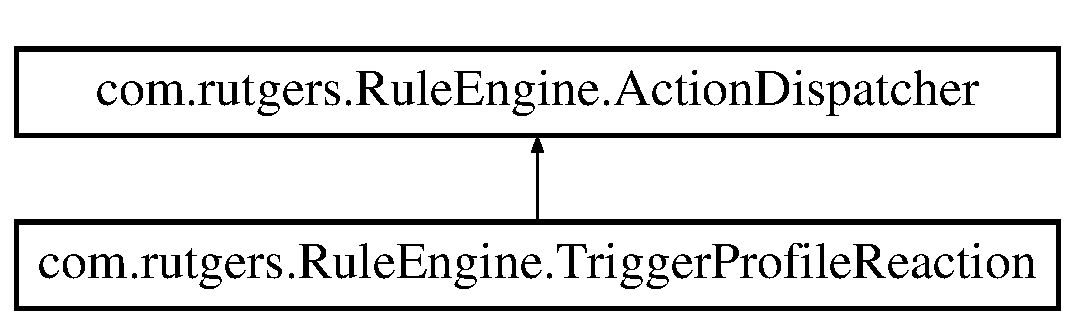
\includegraphics[height=2.000000cm]{classcom_1_1rutgers_1_1RuleEngine_1_1TriggerProfileReaction}
\end{center}
\end{figure}


\subsection{Detailed Description}
This class is used to send a specific AR Profile when a rule is satisfied.

\begin{DoxyAuthor}{Author}
Eduard Giber Renart 
\end{DoxyAuthor}
\begin{DoxyVersion}{Version}
1.\+0 
\end{DoxyVersion}


The documentation for this class was generated from the following file\+:\begin{DoxyCompactItemize}
\item 
src/main/java/com/rutgers/\+Rule\+Engine/Trigger\+Profile\+Reaction.\+java\end{DoxyCompactItemize}

\hypertarget{classcom_1_1rutgers_1_1Encryption_1_1UserProfile}{}\section{com.\+rutgers.\+Encryption.\+User\+Profile Class Reference}
\label{classcom_1_1rutgers_1_1Encryption_1_1UserProfile}\index{com.\+rutgers.\+Encryption.\+User\+Profile@{com.\+rutgers.\+Encryption.\+User\+Profile}}


\subsection{Detailed Description}
\begin{DoxyAuthor}{Author}
eduard 
\end{DoxyAuthor}


The documentation for this class was generated from the following file\+:\begin{DoxyCompactItemize}
\item 
src/main/java/com/rutgers/\+Encryption/User\+Profile.\+java\end{DoxyCompactItemize}

\hypertarget{classcom_1_1rutgers_1_1Core_1_1Utils}{}\section{com.\+rutgers.\+Core.\+Utils Class Reference}
\label{classcom_1_1rutgers_1_1Core_1_1Utils}\index{com.\+rutgers.\+Core.\+Utils@{com.\+rutgers.\+Core.\+Utils}}
\subsection*{Static Public Member Functions}
\begin{DoxyCompactItemize}
\item 
static String \hyperlink{classcom_1_1rutgers_1_1Core_1_1Utils_aedb9187bb0ecf964d125b300774e98d2}{execute\+Command} (String command)
\item 
static byte \mbox{[}$\,$\mbox{]} \hyperlink{classcom_1_1rutgers_1_1Core_1_1Utils_a24dd8f1b7d7608b660646f798c477089}{long\+To\+Byte\+Array} (long value)
\item 
static int \hyperlink{classcom_1_1rutgers_1_1Core_1_1Utils_a052366fc4a329698e13f6c6633467a98}{get\+Max} (int first, int second)
\item 
static byte \mbox{[}$\,$\mbox{]} \hyperlink{classcom_1_1rutgers_1_1Core_1_1Utils_a56a1cd6f67c4f6387826bf38adf6e82f}{write\+File\+To\+Bytes} (String file)  throws I\+O\+Exception 
\end{DoxyCompactItemize}


\subsection{Detailed Description}
This is used to implement miscellaneous tools need it in R-\/\+Pulsar.

\begin{DoxyAuthor}{Author}
Eduard Giber Renart 
\end{DoxyAuthor}
\begin{DoxyVersion}{Version}
1.\+0 
\end{DoxyVersion}


\subsection{Member Function Documentation}
\mbox{\Hypertarget{classcom_1_1rutgers_1_1Core_1_1Utils_aedb9187bb0ecf964d125b300774e98d2}\label{classcom_1_1rutgers_1_1Core_1_1Utils_aedb9187bb0ecf964d125b300774e98d2}} 
\index{com\+::rutgers\+::\+Core\+::\+Utils@{com\+::rutgers\+::\+Core\+::\+Utils}!execute\+Command@{execute\+Command}}
\index{execute\+Command@{execute\+Command}!com\+::rutgers\+::\+Core\+::\+Utils@{com\+::rutgers\+::\+Core\+::\+Utils}}
\subsubsection{\texorpdfstring{execute\+Command()}{executeCommand()}}
{\footnotesize\ttfamily static String com.\+rutgers.\+Core.\+Utils.\+execute\+Command (\begin{DoxyParamCaption}\item[{String}]{command }\end{DoxyParamCaption})\hspace{0.3cm}{\ttfamily [static]}}

Method used to execute linux commands. 
\begin{DoxyParams}{Parameters}
{\em command} & Linux command to execute. \\
\hline
\end{DoxyParams}
\begin{DoxyReturn}{Returns}

\end{DoxyReturn}
\mbox{\Hypertarget{classcom_1_1rutgers_1_1Core_1_1Utils_a052366fc4a329698e13f6c6633467a98}\label{classcom_1_1rutgers_1_1Core_1_1Utils_a052366fc4a329698e13f6c6633467a98}} 
\index{com\+::rutgers\+::\+Core\+::\+Utils@{com\+::rutgers\+::\+Core\+::\+Utils}!get\+Max@{get\+Max}}
\index{get\+Max@{get\+Max}!com\+::rutgers\+::\+Core\+::\+Utils@{com\+::rutgers\+::\+Core\+::\+Utils}}
\subsubsection{\texorpdfstring{get\+Max()}{getMax()}}
{\footnotesize\ttfamily static int com.\+rutgers.\+Core.\+Utils.\+get\+Max (\begin{DoxyParamCaption}\item[{int}]{first,  }\item[{int}]{second }\end{DoxyParamCaption})\hspace{0.3cm}{\ttfamily [static]}}

Get the bigger number given two numbers. 
\begin{DoxyParams}{Parameters}
{\em first} & \\
\hline
{\em second} & \\
\hline
\end{DoxyParams}
\begin{DoxyReturn}{Returns}

\end{DoxyReturn}
\mbox{\Hypertarget{classcom_1_1rutgers_1_1Core_1_1Utils_a24dd8f1b7d7608b660646f798c477089}\label{classcom_1_1rutgers_1_1Core_1_1Utils_a24dd8f1b7d7608b660646f798c477089}} 
\index{com\+::rutgers\+::\+Core\+::\+Utils@{com\+::rutgers\+::\+Core\+::\+Utils}!long\+To\+Byte\+Array@{long\+To\+Byte\+Array}}
\index{long\+To\+Byte\+Array@{long\+To\+Byte\+Array}!com\+::rutgers\+::\+Core\+::\+Utils@{com\+::rutgers\+::\+Core\+::\+Utils}}
\subsubsection{\texorpdfstring{long\+To\+Byte\+Array()}{longToByteArray()}}
{\footnotesize\ttfamily static byte \mbox{[}$\,$\mbox{]} com.\+rutgers.\+Core.\+Utils.\+long\+To\+Byte\+Array (\begin{DoxyParamCaption}\item[{long}]{value }\end{DoxyParamCaption})\hspace{0.3cm}{\ttfamily [static]}}

Convert a long to a byte array. 
\begin{DoxyParams}{Parameters}
{\em value} & \\
\hline
\end{DoxyParams}
\begin{DoxyReturn}{Returns}

\end{DoxyReturn}
\mbox{\Hypertarget{classcom_1_1rutgers_1_1Core_1_1Utils_a56a1cd6f67c4f6387826bf38adf6e82f}\label{classcom_1_1rutgers_1_1Core_1_1Utils_a56a1cd6f67c4f6387826bf38adf6e82f}} 
\index{com\+::rutgers\+::\+Core\+::\+Utils@{com\+::rutgers\+::\+Core\+::\+Utils}!write\+File\+To\+Bytes@{write\+File\+To\+Bytes}}
\index{write\+File\+To\+Bytes@{write\+File\+To\+Bytes}!com\+::rutgers\+::\+Core\+::\+Utils@{com\+::rutgers\+::\+Core\+::\+Utils}}
\subsubsection{\texorpdfstring{write\+File\+To\+Bytes()}{writeFileToBytes()}}
{\footnotesize\ttfamily static byte \mbox{[}$\,$\mbox{]} com.\+rutgers.\+Core.\+Utils.\+write\+File\+To\+Bytes (\begin{DoxyParamCaption}\item[{String}]{file }\end{DoxyParamCaption}) throws I\+O\+Exception\hspace{0.3cm}{\ttfamily [static]}}

Write a string to a File. 
\begin{DoxyParams}{Parameters}
{\em file} & \\
\hline
\end{DoxyParams}
\begin{DoxyReturn}{Returns}

\end{DoxyReturn}

\begin{DoxyExceptions}{Exceptions}
{\em I\+O\+Exception} & \\
\hline
\end{DoxyExceptions}


The documentation for this class was generated from the following file\+:\begin{DoxyCompactItemize}
\item 
src/main/java/com/rutgers/\+Core/Utils.\+java\end{DoxyCompactItemize}

\hypertarget{classcom_1_1rutgers_1_1Core_1_1Wildcard}{}\section{com.\+rutgers.\+Core.\+Wildcard Class Reference}
\label{classcom_1_1rutgers_1_1Core_1_1Wildcard}\index{com.\+rutgers.\+Core.\+Wildcard@{com.\+rutgers.\+Core.\+Wildcard}}


\subsection{Detailed Description}
This class is used to implement the wildcard in the R-\/\+Pulsar profiles.

\begin{DoxyAuthor}{Author}
Eduard Giber Renart 
\end{DoxyAuthor}
\begin{DoxyVersion}{Version}
1.\+0 
\end{DoxyVersion}


The documentation for this class was generated from the following file\+:\begin{DoxyCompactItemize}
\item 
src/main/java/com/rutgers/\+Core/Wildcard.\+java\end{DoxyCompactItemize}

%--- End generated contents ---

% Index
\backmatter
\newpage
\phantomsection
\clearemptydoublepage
\addcontentsline{toc}{chapter}{Index}
\printindex

\end{document}
